% Opciones empleadas:
%
%	a4paper -> indica el tamaño del papel, en este caso A4.
%	11pt -> tamaño de la fuente 11 puntos.
%	oneside -> sólo escribimos en una cara del folio.
% 
% Otras opciones interesantes:
%
%	twoside -> escribimos a doble cara.
%	openbib -> para que las referencias bibliográficas tengan un salto de línea entre cada campo de la referencia.
%
\documentclass[a4paper,oneside,11pt]{book}

\usepackage[spanish,activeacute]{babel}
\usepackage[utf8]{inputenc}
%\usepackage[T1]{fontenc}
\usepackage{tabulary}
\usepackage{graphicx}
\usepackage{color}
\usepackage{colortbl}
\usepackage{float}

% configuración de márgenes
\oddsidemargin=0.2cm
\headsep=1cm
\textheight=21cm
\textwidth=16cm

\setcounter{secnumdepth}{3}

\definecolor{gris}{gray}{0.80}
\definecolor{gris2}{gray}{0.90}
\definecolor{negro}{gray}{0}

% Personalizamos la separación entre párrafos...
\parskip=6pt

% Personalizamos el identado en la primera línea del nuevo párrafo...
\parindent=10pt

\title{\bf Desarrollo Aplicación Web de Gestión de Consultas Médicas Particulares}
\author{Pablo Eduardo Ojeda Vasco}
\date{\today}

\begin{document}
	\maketitle
	
	% Página de agradecimientos
	\newpage 
	\thispagestyle{empty} 
	\section*{}
	\begin{quote}
		{\it En el verdadero éxito, la suerte no tiene nada que ver; la suerte es para los improvisados y aprovechados; y el éxito es el resultado obligado de la constancia, de la responsabilidad, del esfuerzo, de la organización y del equilibrio entre la razón y el corazón.}
	\end{quote}
	
	% Glosario		
	%\makegloss
	
	% FRONTMATTER: TOC, LOF, LOT y descripcion/organizacion de la memoria.
	\frontmatter

	\tableofcontents
	\listoffigures
	\listoftables
	%\include{frontmatter_intro}
	
	% MAINMATTER: El contenido, capitulo a capitulo, de la memoria.
	\mainmatter
	
	% Capítulo de Introducción
\chapter*{Introducción} % (fold)
\label{cha:introduccion}
	El {\bf dominio} de la aplicación es el de las {\bf consultas médicas privadas}, donde normalmente existen {\bf dos actores} principales: el médico y el paciente. Es decir, el proyecto está orientado a médicos que gestionen consultas de carácter particular y a sus pacientes.

		En primer lugar debemos ponernos en situación. En el sector de la sanidad privada, la gestión de centros médicos (desde el seguimiento de un paciente hasta la organización interna del mismo) se ha desarrollado {\bf tradicionalmente en papel} (información analógica). Sin embargo, con el avance tecnológico y con la aparición de las nuevas tecnologías de información y comunicación (TICs), se crean nuevos modelos de gestión y administración de los centros, pasando todos los flujos de datos a versión digital. Es decir, la información comienza a gestionarse usando software específico, pero {\bf centralizado en una localización física concreta}. A pesar de todo, sigue habiendo muchos especialistas que no han dado el paso y continúan utilizando métodos arcaicos.

		Por otro lado, {\bf el proceso de concertar una cita} sigue siendo el mismo que antaño: un paciente debe presentarse en la consulta del médico físicamente y solicitar cita ó bien debe realizar una llamada telefónica para ser atendido por un administrativo.

		Por tanto, con el objetivo de poder gestionar digitalmente y desde “la nube” todos los aspectos referentes al flujo de información de una consulta médica, se requiere desarrollar una aplicación web desde la que se gestionen un gran número de consultas privadas, con todos los datos referentes a médicos (curriculum, precios, horarios de disponibilidad, etc.), a pacientes (ficha médica, diagnósticos, pruebas, exploraciones, etc.), los pagos y el seguimiento de la contabilidad y además, permita que sean los propios especialistas los que muestren a los pacientes de que horas libres disponen, para que sean estos últimos los encargados de asignarse, desde cualquier ubicación en la que exista un computador con internet, la cita que más les convenga.
% chapter introducción (end) % Introducción
	
	% Análisis
	\chapter{Análisis} % (fold)
	\label{cha:analisis}
		\section{Descripción general del proyecto} % (fold)
\label{sec:descripcion_general_del_proyecto}
    % Usuarios
	\subsection {Usuarios}
	En primer lugar se muestra una clasificación de los posibles usuarios del sistema. De esta forma podremos identificar y asociar cada característica con cada uno de ellos. 

	\begin{itemize}
	\item \textbf{Médicos.} A ellos está dedicada la aplicación. Pueden tener cualquier tipo de especialidad.
	\item \textbf{Pacientes.} No son los usuarios principales del sistema, pero son el sustento de los médicos. Pueden interactuar con el software a la hora de reservar citas o de realizar pagos por adelantado.
	\item \textbf{Administrador del sistema.} Encargado de verificar que el sistema funciona correctamente. Además, debe verificar que un médico esté licenciado como tal y realizar las copias de seguridad.
	\end{itemize}

	% Objetivos
	\subsection{Objetivos}
	Se propone diseñar e implementar una aplicación SaaS (Software as a Service), que lo que pretende es ofertar un {\bf software como servicio} a todos aquellos especialistas sanitarios interesados. 

		Por tanto, se desarrollará una aplicación web, en la que se abordaran los siguientes módulos:
	\begin{itemize}
		\item \textbf{Gestión de médicos.} Funcionalidades que pueden desarrollar los distintos especialistas para gestionar su consulta de la forma más eficiente posible. Tienen que ver principalmente con su calendario, sus plantillas, sus pacientes y con diversos datos de configuración.
		\item \textbf{Gestión de pacientes.} Funcionalidades que pueden desarrollar los usuarios con el rol de paciente. Tienen que ver principalmente con sus citas, sus médicos, con diversos datos de configuración y con la información de sus fichas médicas.
		\item \textbf{Gestión de fichas médicas.} Ficha médica de los pacientes, con sus pruebas médicas, diagnósticos, tratamientos, informes, información asociada, etcétera.
		\item \textbf{Panel de administrador.} El sistema será gestionado y mantenido por un administrador, el cuál podrá realizar diversas tareas.
		\item \textbf{Gestión de actividades generales.} Una serie de funcionalidades que podrán realizar usuarios sin necesidad de estar identificados, tales como darse de alta en la aplicación, ver las condiciones generales, un tour de la aplicación, buscar si un médico forma parte del sistema, etcétera.
	\end{itemize}
	 
% subsection descripción_general_del_proyecto (end)
 % Descripcion general
		\section{Lista de características} % (fold)
\label{sec:lista_de_caracteristicas}

	La lista de características es un artefacto que se obtiene después de aplicar la tarea de “Enumerar los requisitos candidatos”, que se propone en la metodología del PUD (Proceso Unificado de Desarrollo), para la captura de requisitos. 

		Esta lista contiene las ideas de clientes, usuarios, analistas y desarrolladores sobre posibles aspectos que se podrían incluir en la aplicación, y que, posteriormente, se podrán traducir en requisitos del software. 

		Estas ideas se consideran requisitos candidatos que se podrán desarrollar en la versión actual del sistema o se podrán postergar a versiones futuras. Este artefacto sirve para gestionar el proyecto y sólo se utiliza para la planificación del trabajo. Podrá ir variando a medida que avance el proyecto, pudiéndose añadir y modificar las características que se crean oportunas, en cualquier momento del desarrollo.

	% 1.3.1.- Descripción de las características
	\subsection{Descripción de las características}
	Para describir cada una de las características vamos a utilizar los siguientes campos:

	\begin{itemize}
	\item \textbf{Código.} Identifica a la característica. Se especifica como Categoría + Número. Las categorías se especifican más abajo.
	\item \textbf{Nombre.} El nombre de la característica.
	\item \textbf{Descripción.} Breve descripción de lo que comprende la característica.
	\item \textbf{Estado.} Cada característica tendrá un estado que irá variando a medida que progrese el proyecto. Los posibles estados son:
		\begin{itemize}
			\item Aceptado. Se desarrollará en esta versión del producto.
			\item Rechazado. No se desarrollará.
			\item Postergado. Se desarrollará en una futura versión.
			\item En desarrollo. Ya se está desarrollando.
			\item Finalizado. Se ha concluido.
		\end{itemize}
	\item \textbf{Prioridad.} Determinará el orden en el que se van a ir desarrollando. Los tipos de prioridades son:
		\begin{itemize}
			\item Muy alta.
			\item Alta.
			\item Media.
			\item Baja.
			\item Muy Baja.
		\end{itemize}
	\item \textbf{Riesgo.} Representa la dificultad para conseguir implementar la característica correctamente. Existen tres niveles: 
		\begin{itemize}
			\item Crítico
			\item Significativo
			\item Rutinario.
		\end{itemize}
	\end{itemize}

	% 1.3.2.- Categorías
	\subsection{Categorías}
	Para organizar la lista tenemos una serie de categorías que se mencionan a continuación. Gracias a esto podremos gestionar mejor la lista de características.
	\begin{itemize}
	\item [A].- Gestión de Actividades Generales 
	\item [B].- Gestión de información de médicos.
	\item [C].- Actividades de los médicos.
	\item [D].- Gestión de pacientes.
	\item [E].- Gestión de fichas médicas de pacientes.
	\item [F].- Gestión de horarios de los médicos.
	\item [G].- Gestión de citas de los pacientes.
	\item [H].- Consulta y Diagnósticos.
	\item [I].- Gestión de cobros y pagos.
	\item [J].- Gestión de contabilidad.
	\item [K].- Panel de Administrador.
	\item [L].- Otros
	\end{itemize}

	% 1.3.3.- Lista de características
	\subsection{Lista de características}

	%%%%%%%
	% A - Gestión de actividades generales
	%%%%%%%
	\subsubsection{A.- Gestión de actividades generales.}

	%\begin{table}
	\begin{center}
	\begin{tabulary}{15cm}{|L|}
		\hline
			\bf{A.1.- Tour de la Aplicación} \\
		\hline
			Cualquier médico ó paciente podrá hacer una visita guiada sobre las principales funcionalidades de la aplicación.\\
		\hline
			Prioridad \textit{Postergado.} \\
		\hline
			Estado \textit{Medio.} \\
		\hline
			Riesgo \textit{Riguroso.} \\
		\hline
	\end{tabulary}
	\end{center}
	%\caption{XXX}
	%\end{table}

	%\begin{table}
	\begin{center}
	\begin{tabulary}{15cm}{|L|}
		\hline
			\bf{A.2.- Registrarse como médico} \\
		\hline
			Un médico deberá registrarse como tal. Se pasará a rellenar una serie de datos correspondientes con su información personal, profesional, etc. El usuario será el e-mail seleccionado, y su contraseña la elegida.\\
		\hline
			Prioridad \textit{Aceptado.} \\
		\hline
			Estado \textit{Muy Alta.} \\
		\hline
			Riesgo \textit{Significativo.} \\
		\hline
	\end{tabulary}
	\end{center}
	%\caption{XXX}
	%\end{table}

	%\begin{table}
	\begin{center}
	\begin{tabulary}{15cm}{|L|}
		\hline
			\bf{A.3.- Registrarse como paciente.} \\
		\hline
			Un paciente deberá registrarse como tal. Se pasará a rellenar una serie de datos correspondientes con su información personal, sus historial médico, etc. El usuario será el e-mail seleccionado y su contraseña la elegida. \\
		\hline
			Prioridad \textit{Aceptado.} \\
		\hline
			Estado \textit{Muy Alta.} \\
		\hline
			Riesgo \textit{Significativo.} \\
		\hline
	\end{tabulary}
	\end{center}
	%\caption{XXX}
	%\end{table}

	%\begin{table}
	\begin{center}
	\begin{tabulary}{15cm}{|L|}
		\hline
			\bf{A.4.- Registrarse como administrativo.} \\
		\hline
			Un administrativo deberá registrarse como tal. El usuario será el e-mail seleccionado y su contraseña la elegida. Deberá permanecer a la espera de que su médico le autorice. \\
		\hline
			Prioridad \textit{Rechazado.} \\
		\hline
			Estado \textit{Baja.} \\
		\hline
			Riesgo \textit{Significativo.} \\
		\hline
	\end{tabulary}
	\end{center}
	%\caption{XXX}
	%\end{table}

	%\begin{table}
	\begin{center}
	\begin{tabulary}{15cm}{|L|}
		\hline
			\bf{A.5.- Rellenar información personal.} \\
		\hline
			Tanto médicos como pacientes debe rellenar todos sus datos personales cuando ingresen en el sistema. Nombre, apellidos, DNI, teléfono de contacto, e-mail, etc. \\
		\hline
			Prioridad \textit{Aceptado.} \\
		\hline
			Estado \textit{Muy Alta.} \\
		\hline
			Riesgo \textit{Riguroso.} \\
		\hline
	\end{tabulary}
	\end{center}
	%\caption{XXX}
	%\end{table}

	%\begin{table}
	\begin{center}
	\begin{tabulary}{15cm}{|L|}
		\hline
			\bf{A.6.- Modificar información personal.} \\	
		\hline
			Tanto médicos como pacientes debe poder cambiar algunos de sus datos personales en cualquier momento que desee. \\
		\hline
			Prioridad \textit{Aceptado.} \\
		\hline
			Estado \textit{Media.} \\
		\hline
			Riesgo \textit{Riguroso.} \\
		\hline
	\end{tabulary}
	\end{center}
	%\caption{XXX}
	%\end{table}

	%\begin{table}
	\begin{center}
	\begin{tabulary}{15cm}{|L|}
		\hline
			\bf{A.7.- Adjuntar foto del perfil.} \\
		\hline
			Es recomendable que todos los médicos y pacientes tengan una foto del perfil. Respecto a los médicos da mayor seguridad y credibilidad a sus futuros pacientes potenciales. Respecto a los pacientes, permite que los médicos puedan poner cara a la hora de ver los datos. \\
		\hline
			Prioridad \textit{Aceptado.} \\
		\hline
			Estado \textit{Alta.} \\
		\hline
			Riesgo \textit{Riguroso.} \\
		\hline
	\end{tabulary}
	\end{center}
	%\caption{XXX}
	%\end{table}

	%\begin{table}
	\begin{center}
	\begin{tabulary}{15cm}{|L|}
		\hline
			\bf{A.8.- Modificar foto del perfil.} \\
		\hline
			Tanto médicos como pacientes pueden modificar la foto de su perfil en cualquier momento que desee. Para modificarla deben primero haberla adjuntado. \\
		\hline
			Prioridad \textit{Aceptado.} \\
		\hline
			Estado \textit{Media.} \\
		\hline
			Riesgo \textit{Riguroso.} \\
		\hline
	\end{tabulary}
	\end{center}
	%\caption{XXX}
	%\end{table}

	%\begin{table}
	\begin{center}
	\begin{tabulary}{15cm}{|L|}
		\hline
			\bf{A.9.- Acceso y Autentificación.} \\
		\hline
			Una vez registrado en el sistema, tanto médico, pacientes como administrador deben autentificarse mediante su usuario y contraseña para poder acceder a la aplicación. \\
		\hline
			Prioridad \textit{Aceptado.} \\
		\hline
			Estado \textit{Muy Alta.} \\
		\hline
			Riesgo \textit{Significativo.} \\
		\hline
	\end{tabulary}
	\end{center}
	%\caption{XXX}
	%\end{table}

	%\begin{table}
	\begin{center}
	\begin{tabulary}{15cm}{|L|}
		\hline
			\bf{A.10.- Conectarse desde cuenta Facebook.} \\
		\hline
			Un usuario también podrá acceder con su usuario y contraseña de acceso a Facebook. Esto no quita que deba seguir rellenando su información personal y otra serie de datos. \\
		\hline
			Prioridad \textit{Rechazado.} \\
		\hline
			Estado \textit{Baja.} \\
		\hline
			Riesgo \textit{Riguroso.} \\
		\hline
	\end{tabulary}
	\end{center}
	%\caption{XXX}
	%\end{table}

	%\begin{table}
	\begin{center}
	\begin{tabulary}{15cm}{|L|}
		\hline
			\bf{A.11.- Recordar contraseña.} \\
		\hline
			Se establece la opción de que el propio navegador recuerde el usuario y la contraseña para que se acceda directamente al sistema sin tener que estar continuamente introduciendo dicha información. \\
		\hline
			Prioridad \textit{Aceptado.} \\
		\hline
			Estado \textit{Media.} \\
		\hline
			Riesgo \textit{Significativo.} \\
		\hline
	\end{tabulary}
	\end{center}
	%\caption{XXX}
	%\end{table}

	%\begin{table}
	\begin{center}
	\begin{tabulary}{15cm}{|L|}
		\hline
			\bf{A.12.- Cambiar contraseña.} \\
		\hline
			En cualquier momento que desee, tanto médicos, pacientes como el administrador del sistema podrán cambiar su contraseña de acceso al sistema. Se pedirá contraseña actual para corroborar que es la persona que dice ser y la nueva contraseña deberá introducirse dos veces para evitar errores al teclear. \\
		\hline
			Prioridad \textit{Aceptado.} \\
		\hline
			Estado \textit{Media.} \\
		\hline
			Riesgo \textit{Riguroso.} \\
		\hline
	\end{tabulary}
	\end{center}
	%\caption{XXX}
	%\end{table}

	%\begin{table}
	\begin{center}
	\begin{tabulary}{15cm}{|L|}
		\hline
			\bf{A.13.- Cambiar idioma.} \\
		\hline
			Un usuario del sistema, tanto médico, paciente o administrador, podrá cambiar el idioma de la aplicación. \\
		\hline
			Prioridad \textit{Postergado.} \\
		\hline
			Estado \textit{Baja.} \\
		\hline
			Riesgo \textit{Crítico.} \\
		\hline
	\end{tabulary}
	\end{center}
	%\caption{XXX}
	%\end{table}

	%\begin{table}
	\begin{center}
	\begin{tabulary}{15cm}{|L|}
		\hline
			\bf{A.14.- Contactar con el Administrador.} \\
		\hline
			En caso de cualquier consulta o problema, los médicos podrán enviar directamente un email al administrador. \\
		\hline
			Prioridad \textit{Aceptado.} \\
		\hline
			Estado \textit{Medio.} \\
		\hline
			Riesgo \textit{Riguroso.} \\
		\hline
	\end{tabulary}
	\end{center}
	%\caption{XXX}
	%\end{table}

	%\begin{table}
	\begin{center}
	\begin{tabulary}{15cm}{|L|}
		\hline
			\bf{A.15.- Términos Legales.} \\
		\hline
			Se expondrán todos los términos legales accesibles para todo el mundo, tanto registrado en el sistema como ajeno a éste. \\
		\hline
			Prioridad \textit{Aceptado.} \\
		\hline
			Estado \textit{Alta.} \\
		\hline
			Riesgo \textit{Riguroso.} \\
		\hline
	\end{tabulary}
	\end{center}
	%\caption{XXX}
	%\end{table}

	%\begin{table}
	\begin{center}
	\begin{tabulary}{15cm}{|L|}
		\hline
			\bf{A.16.- Condiciones de uso.} \\
		\hline
			Una lista de características con las condiciones de uso del sistema con las que se informará a sus usuarios de todo tipo de detalles respecto a cualquier detalle relacionado con su utilización. \\
		\hline
			Prioridad \textit{Aceptado.} \\
		\hline
			Estado \textit{Alta.} \\
		\hline
			Riesgo \textit{Riguroso.} \\
		\hline
	\end{tabulary}
	\end{center}
	%\caption{XXX}
	%\end{table}

	%\begin{table}
	\begin{center}
	\begin{tabulary}{15cm}{|L|}
		\hline
			\bf{A.17.- Autocompletar las búsquedas.} \\
		\hline
			Cualquier búsqueda que se realice en el sistema, bien por parte del paciente, del médico o del administrador, se realizará mediante el autocompletado, de forma que se aconseje al usuario sobre las posibles búsquedas posibles. \\
		\hline
			Prioridad \textit{Postergado.} \\
		\hline
			Estado \textit{Alta.} \\
		\hline
			Riesgo \textit{Crítico.} \\
		\hline
	\end{tabulary}
	\end{center}
	%\caption{XXX}
	%\end{table}

	%\begin{table}
	\begin{center}
	\begin{tabulary}{15cm}{|L|}
		\hline
			\bf{A.18.- Ayuda.} \\
		\hline
			En cualquier momento, cualquier usuario podrá solicitar ayuda sobre cualquier funcionalidad. Además, en cada icono del interfaz gráfica aparecerá al pasar el ratón por encima cuál es su uso. \\
		\hline
			Prioridad \textit{Aceptado.} \\
		\hline
			Estado \textit{Baja.} \\
		\hline
			Riesgo \textit{Crítico.} \\
		\hline
	\end{tabulary}
	\end{center}
	%\caption{XXX}
	%\end{table}


	%%%%%%%%%%
	% B - Gestión de información de médicos
	%%%%%%%%%%
	\subsubsection{B.- Gestión de información de médicos.}

	%\begin{table}
	\begin{center}
	\begin{tabulary}{15cm}{|L|}
		\hline
			\bf{B.1.- Rellenar número de colegiado.} \\
		\hline
			Cualquier médico debe tener asociado un número de colegiado en el Colegio de Médicos. Dicho identificador debe ser añadido \\
		\hline
			Prioridad \textit{Aceptado.} \\
		\hline
			Estado \textit{Alta.} \\
		\hline
			Riesgo \textit{Riguroso.} \\
		\hline
	\end{tabulary}
	\end{center}
	%\caption{XXX}
	%\end{table}

	%\begin{table}
	\begin{center}
	\begin{tabulary}{15cm}{|L|}
		\hline
			\bf{B.2.- Rellenar información del centro (localización, contacto).} \\
		\hline
			Es necesario que un paciente conozca la ubicación de la consulta del médico. Así mismo, debe tener unos datos de contacto, un CIF, etc. \\
		\hline
			Prioridad \textit{Aceptado.} \\
		\hline
			Estado \textit{Alta.} \\
		\hline
			Riesgo \textit{Riguroso.} \\
		\hline
	\end{tabulary}
	\end{center}
	%\caption{XXX}
	%\end{table}

	%\begin{table}
	\begin{center}
	\begin{tabulary}{15cm}{|L|}
		\hline
			\bf{B.3.- Adjuntar curriculum.} \\
		\hline
			Se oferta la posibilidad de que un médico adjunte su curriculum en caso de que disponga de este en formato digital. \\ 
		\hline
			Prioridad \textit{Aceptado.} \\
		\hline
			Estado \textit{Alto.} \\
		\hline
			Riesgo \textit{Riguroso.} \\
		\hline
	\end{tabulary}
	\end{center}
	%\caption{XXX}
	%\end{table}

	%\begin{table}
	\begin{center}
	\begin{tabulary}{15cm}{|L|}
		\hline
			\bf{B.4.- Crear curriculum.} \\
		\hline
			En el caso de no tener un curriculum en formato digital, o de no poder escanear uno, se ofrece la posibilidad de crear su propio curriculum. \\
		\hline
			Prioridad \textit{Postergado.} \\
		\hline
			Estado \textit{Baja.} \\
		\hline
			Riesgo \textit{Significativo.} \\
		\hline
	\end{tabulary}
	\end{center}
	%\caption{XXX}
	%\end{table}


	%%%%%%%%%%
	% C - Actividades de los médicos
	%%%%%%%%%%
	\subsubsection{C.- Actividades de los médicos.}

	%\begin{table}
	\begin{center}
	\begin{tabulary}{15cm}{|L|}
		\hline
			\bf{C.1.- Enviar certificación de licencia médica.} \\
		\hline
			Para poder corroborar que un médico tiene licencia médica, éste debe mandar una copia de su título, su número de colegiado, etc. \\
		\hline
			Prioridad \textit{Aceptado.} \\
		\hline
			Estado \textit{Muy Alta.} \\
		\hline
			Riesgo \textit{Significativo.} \\
		\hline
	\end{tabulary}
	\end{center}
	%\caption{XXX}
	%\end{table}

	%\begin{table}
	\begin{center}
	\begin{tabulary}{15cm}{|L|}
		\hline
			\bf{C.2.- Abonar cuota del servicio.} \\
		\hline
			Un médico debe pagar mensualmente o anualmente una cuota establecida por utilizar el servicio. \\
		\hline
			Prioridad \textit{Aceptado.} \\
		\hline
			Estado \textit{Muy Alta.} \\
		\hline
			Riesgo \textit{Crítcio.} \\
		\hline
	\end{tabulary}
	\end{center}
	%\caption{XXX}
	%\end{table}

	%\begin{table}
	\begin{center}
	\begin{tabulary}{15cm}{|L|}
		\hline
			\bf{C.3.- Darse de baja en el servicio.} \\
		\hline
			En el caso de que un médico ya no quiera volver a utilizar el servicio, debe darse de baja. \\
		\hline
			Prioridad \textit{Aceptado.} \\
		\hline
			Estado \textit{Alta.} \\
		\hline
			Riesgo \textit{Significativo.} \\
		\hline
	\end{tabulary}
	\end{center}
	%\caption{XXX}
	%\end{table}

	%\begin{table}
	\begin{center}
	\begin{tabulary}{15cm}{|L|}
		\hline
			\bf{C.4.- Generar plantilla básica a rellenar para su consulta.} \\
		\hline
			En el caso de que un médico lo vea oportuno, podrá generar una plantilla con una serie de preguntas específicas que el paciente deberá responder en el momento en el que solicite una cita. \\
		\hline
			Prioridad \textit{Postergado.} \\
		\hline
			Estado \textit{Medio.} \\
		\hline
			Riesgo \textit{Significativo.} \\
		\hline
	\end{tabulary}
	\end{center}
	%\caption{XXX}
	%\end{table}

	%\begin{table}
	\begin{center}
	\begin{tabulary}{15cm}{|L|}
		\hline
			\bf{C.5.- Registrar administrativos en la consulta.} \\
		\hline
			En el caso de que un médico cuente con personal de administración, éste debe registrar a un administrativo y darle un nombre de usuario y una contraseña que podrá ser cambiada por el propio trabajador. \\
		\hline
			Prioridad \textit{Rechazado.} \\
		\hline
			Estado \textit{Baja.} \\
		\hline
			Riesgo \textit{Significativo.} \\
		\hline
	\end{tabulary}
	\end{center}
	%\caption{XXX}
	%\end{table}

	%\begin{table}
	\begin{center}
	\begin{tabulary}{15cm}{|L|}
		\hline
			\bf{C.6.- Eliminar administrativo de la consulta.} \\
		\hline
			En el caso de que un médico cuente con personal de administración, y vaya a prescindir de sus servicios, podrá darlo de baja en el sistema en cualquier momento. \\
		\hline
			Prioridad \textit{Rechazado.} \\
		\hline
			Estado \textit{Muy Baja.} \\
		\hline
			Riesgo \textit{Riguroso.} \\
		\hline
	\end{tabulary}
	\end{center}
	%\caption{XXX}
	%\end{table}

	%%%%%%%%%%
	% D - Gestión de pacientes
	%%%%%%%%%%
	\subsubsection{D.- Gestión de pacientes.}

	%\begin{table}
	\begin{center}
	\begin{tabulary}{15cm}{|L|}
		\hline
			\bf{D.1.- Elegir médicos favoritos.} \\
		\hline
			Un paciente puede tener una lista con accesos a sus médicos favoritos, que serán, posiblemente, aquellos que visite con más frecuencia. \\
		\hline
			Prioridad \textit{Aceptado.} \\
		\hline
			Estado \textit{Medio.} \\
		\hline
			Riesgo \textit{Significativo.} \\
		\hline
	\end{tabulary}
	\end{center}
	%\caption{XXX}
	%\end{table}

	%\begin{table}
	\begin{center}
	\begin{tabulary}{15cm}{|L|}
		\hline
			\bf{D.2.- Votar médicos.} \\
		\hline
			Para conocer opiniones sobre otros médicos y recomendárselo a otros usuarios, un paciente, después de haber tenido una cita con un médico, podrá evaluarlo y escribir un comentario acerca de éste. \\
		\hline
			Prioridad \textit{Postergado.} \\
		\hline
			Estado \textit{Baja.} \\
		\hline
			Riesgo \textit{Riguroso.} \\
		\hline
	\end{tabulary}
	\end{center}
	%\caption{XXX}
	%\end{table}

	%\begin{table}
	\begin{center}
	\begin{tabulary}{15cm}{|L|}
		\hline
			\bf{D.3.- Rellenar datos de ficha médica.} \\
		\hline
			Aunque se verán en más detalle en otra categoría los aspectos relevantes a las fichas médicas, un paciente tendrá la característica de poder rellenar su ficha médica. \\
		\hline
			Prioridad \textit{Aceptado.} \\
		\hline
			Estado \textit{Muy Alta.} \\
		\hline
			Riesgo \textit{Significativo.} \\
		\hline
	\end{tabulary}
	\end{center}
	%\caption{XXX}
	%\end{table}

	%\begin{table}
	\begin{center}
	\begin{tabulary}{15cm}{|L|}
		\hline
			\bf{D.4.- Modificar datos de ficha médica.} \\
		\hline
			Un paciente podrá modificar los datos de su ficha médica en cualquier momento que lo desee. Por norma general será para añadir nuevas pruebas. \\
		\hline
			Prioridad \textit{Aceptado.} \\
		\hline
			Estado \textit{Muy Alta.} \\
		\hline
			Riesgo \textit{Significativo.} \\
		\hline
	\end{tabulary}
	\end{center}
	%\caption{XXX}
	%\end{table}

	%%%%%%%%%%
	% E - Gestión de fichas médicas de pacientes
	%%%%%%%%%%
	\subsubsection{E.- Gestión de fichas médicas de pacientes.}

	%\begin{table}
	\begin{center}
	\begin{tabulary}{15cm}{|L|}
		\hline
			\bf{E.1.- Visualizar ficha médica.} \\
		\hline
			Un médico podrá visualizar cuando le sea necesario la información de un paciente con todo su historial. Un paciente también podrá ver y gestionar su ficha en cualquier momento. \\
		\hline
			Prioridad \textit{Aceptado.} \\
		\hline
			Estado \textit{Alta.} \\
		\hline
			Riesgo \textit{Significativo.} \\
		\hline
	\end{tabulary}
	\end{center}
	%\caption{XXX}
	%\end{table}

	%\begin{table}
	\begin{center}
	\begin{tabulary}{15cm}{|L|}
		\hline
			\bf{E.2.- Exportar ficha médica.} \\
		\hline
			Si fuera necesario, un paciente podrá exportar los datos de su ficha en formato pdf para llevarlos a donde desee. \\
		\hline
			Prioridad \textit{Postergado.} \\
		\hline
			Estado \textit{Baja.} \\
		\hline
			Riesgo \textit{Riguroso.} \\
		\hline
	\end{tabulary}
	\end{center}
	%\caption{XXX}
	%\end{table}

	%\begin{table}
	\begin{center}
	\begin{tabulary}{15cm}{|L|}
		\hline
			\bf{E.3.- Imprimir ficha médica.} \\
		\hline
			Un médico y un paciente podrán imprimir en papel los datos que sean necesarios de una ficha si las circunstancias lo requieren. \\
		\hline
			Prioridad \textit{Postergada.} \\
		\hline
			Estado \textit{Baja.} \\
		\hline
			Riesgo \textit{Riguroso.} \\
		\hline
	\end{tabulary}
	\end{center}
	%\caption{XXX}
	%\end{table}

	%\begin{table}
	\begin{center}
	\begin{tabulary}{15cm}{|L|}
		\hline
			\bf{E.4.- Enviar ficha médica.} \\
		\hline
			Un paciente podrá mandar todos los datos de su ficha médica vía e-mail a quien desee. Debe mandar su historial completo. \\
		\hline
			Prioridad \textit{Postergado.} \\
		\hline
			Estado \textit{Baja.} \\
		\hline
			Riesgo \textit{Riguroso.} \\
		\hline
	\end{tabulary}
	\end{center}
	%\caption{XXX}
	%\end{table}

	%\begin{table}
	\begin{center}
	\begin{tabulary}{15cm}{|L|}
		\hline
			\bf{E.5.- Rellenar datos fisiológicos.} \\
		\hline
			El médico, o el propio paciente, podrán rellenar una serie de datos fisiológicos, referentes a la altura, peso, temperatura, tensión, pulso, alergias, enfermedades hereditarias, etc. \\
		\hline
			Prioridad \textit{Aceptado.} \\
		\hline
			Estado \textit{Alta.} \\
		\hline
			Riesgo \textit{Riguroso.} \\
		\hline
	\end{tabulary}
	\end{center}
	%\caption{XXX}
	%\end{table}

	%\begin{table}
	\begin{center}
	\begin{tabulary}{15cm}{|L|}
		\hline
			\bf{E.6.- Añadir análisis.} \\
		\hline
			Un paciente podrá añadir sus últimos análisis. Éstos se guardar en un historial, por fechas, de manera que siempre se puedan consultar análisis anteriores. \\
		\hline
			Prioridad \textit{Aceptado.} \\
		\hline
			Estado \textit{Medio.} \\
		\hline
			Riesgo \textit{Riguroso.} \\
		\hline
	\end{tabulary}
	\end{center}
	%\caption{XXX}
	%\end{table}

	%\begin{table}
	\begin{center}
	\begin{tabulary}{15cm}{|L|}
		\hline
			\bf{E.7.- Añadir Informes.} \\
		\hline
			Un paciente podrá añadir informes de otros especialistas. Éstos se guardar en un historial, por fechas, de manera que siempre se puedan consultar informes anteriores. \\
		\hline
			Prioridad \textit{Aceptado.} \\
		\hline
			Estado \textit{Medio.} \\
		\hline
			Riesgo \textit{Riguroso.} \\
		\hline
	\end{tabulary}
	\end{center}
	%\caption{XXX}
	%\end{table}

	%\begin{table}
	\begin{center}
	\begin{tabulary}{15cm}{|L|}
		\hline
			\bf{E.8.- Añadir Radiografías.} \\
		\hline
			Un paciente podrá añadir sus últimas radiografías y electromiografías. Éstas se guardar en un historial, por fechas, de manera que siempre se puedan consultar las anteriores. \\
		\hline
			Prioridad \textit{Aceptado.} \\
		\hline
			Estado \textit{Medio.} \\
		\hline
			Riesgo \textit{Crítico.} \\
		\hline
	\end{tabulary}
	\end{center}
	%\caption{XXX}
	%\end{table}

	%\begin{table}
	\begin{center}
	\begin{tabulary}{15cm}{|L|}
		\hline
			\bf{E.9.- Añadir diagnóstico.} \\
		\hline
			Un paciente o un médico podrán añadir el diagnóstico que surge como resultado de una cita. Éstos se guardarán en un historial, por fechas, de manera que siempre se puedan consultar informes anteriores. \\
		\hline
			Prioridad \textit{Aceptado.} \\
		\hline
			Estado \textit{Muy Alto.} \\
		\hline
			Riesgo \textit{Significativo.} \\
		\hline
	\end{tabulary}
	\end{center}
	%\caption{XXX}
	%\end{table}

	%\begin{table}
	\begin{center}
	\begin{tabulary}{15cm}{|L|}
		\hline
			\bf{E.10.- Buscar ficha por paciente.} \\
		\hline
			En el caso de que sea necesario, un médico podrá buscar la ficha de un paciente que ya haya sido visitado por él, tanto por el nombre ó apellidos como por el DNI. \\
		\hline
			Prioridad \textit{Aceptado.} \\
		\hline
			Estado \textit{Alta.} \\
		\hline
			Riesgo \textit{Significativo.} \\
		\hline
	\end{tabulary}
	\end{center}
	%\caption{XXX}
	%\end{table}

	%\begin{table}
	\begin{center}
	\begin{tabulary}{15cm}{|L|}
		\hline
			\bf{E.11.- Buscar ficha por enfermedad.} \\
		\hline
			En el caso de que sea necesario, un médico podrá buscar la ficha de aquellos pacientes que ya hayan sido visitados por él, en función de un conjunto de una o varias enfermedades. \\
		\hline
			Prioridad \textit{Postergado.} \\
		\hline
			Estado \textit{Media.} \\
		\hline
			Riesgo \textit{Significativo.} \\
		\hline
	\end{tabulary}
	\end{center}
	%\caption{XXX}
	%\end{table}

	%\begin{table}
	\begin{center}
	\begin{tabulary}{15cm}{|L|}
		\hline
			\bf{E.12.- Pendiente de pruebas.} \\
		\hline
			Un paciente tendrá un estado que indique que está pendiente de pruebas, cuales son y por qué especialista fueron solicitadas. \\
		\hline
			Prioridad \textit{Aceptado.} \\
		\hline
			Estado \textit{Muy Alta.} \\
		\hline
			Riesgo \textit{Significativo.} \\
		\hline
	\end{tabulary}
	\end{center}
	%\caption{XXX}
	%\end{table}

	%\begin{table}
	\begin{center}
	\begin{tabulary}{15cm}{|L|}
		\hline
			\bf{E.13.- Historial de citas.} \\
		\hline
			En la ficha de cada paciente existirá un historial de citas, en el que aparecerán la fecha, el especialista, el tratamiento recomendado por el médico y cuanto ha sido el coste de la consulta. Éste historial es visible para el paciente, sin embargo, cada médico sólo podrá ver la parte en la que él ha estado implicado. \\
		\hline
			Prioridad \textit{Aceptado.} \\
		\hline
			Estado \textit{Muy Alta.} \\
		\hline
			Riesgo \textit{Significativo.} \\
		\hline
	\end{tabulary}
	\end{center}
	%\caption{XXX}
	%\end{table}

	%\begin{table}
	\begin{center}
	\begin{tabulary}{15cm}{|L|}
		\hline
			\bf{E.14.- Firmar Ley de Protección de Datos.} \\
		\hline
			Todo paciente debe estar en conocimiento de que el sistema cumple con la ley de protección de datos, y que su información no podrá ser vista excepto por aquellos especialistas por los que está siendo tratado. Dicha información debe ser firmada o validada por el paciente. \\
		\hline
			Prioridad \textit{Aceptado.} \\
		\hline
			Estado \textit{Muy Alta.} \\
		\hline
			Riesgo \textit{Riguroso.} \\
		\hline
	\end{tabulary}
	\end{center}
	%\caption{XXX}
	%\end{table}

	%\begin{table}
	\begin{center}
	\begin{tabulary}{15cm}{|L|}
		\hline
			\bf{E.15.- Pedir permiso para sacar fotos.} \\
		\hline
			Hay ocasiones en las que es interesante para el médico sacar fotos de las anomalías que presenta el paciente. Para ello, éste último debe dar su consentimiento. Dichas fotos se actualizarán en la ficha del paciente. \\
		\hline
			Prioridad \textit{Postergado.} \\
		\hline
			Estado \textit{Baja.} \\
		\hline
			Riesgo \textit{Significativo.} \\
		\hline
	\end{tabulary}
	\end{center}
	%\caption{XXX}
	%\end{table}


	%%%%%%%%%%
	% F - Gestión de horarios del médico.
	%%%%%%%%%%
	\subsubsection{F.- Gestión de horarios del médico.}

	%\begin{table}
	\begin{center}
	\begin{tabulary}{15cm}{|L|}
		\hline
			\bf{F.1.- Generar horario de disponibilidad.} \\
		\hline
			Para permitir que los pacientes soliciten hora, lo primer que debe hacer un médico es generar su horario de disponibilidad. Deberá seleccionar qué días y a qué horas va a trabajar. \\
		\hline
			Prioridad \textit{Aceptado.} \\
		\hline
			Estado \textit{Muy Alta.} \\
		\hline
			Riesgo \textit{Crítcio.} \\
		\hline
	\end{tabulary}
	\end{center}
	%\caption{XXX}
	%\end{table}

	%\begin{table}
	\begin{center}
	\begin{tabulary}{15cm}{|L|}
		\hline
			\bf{F.2.- Modificar horario de disponibilidad.} \\
		\hline
			Si el médico decide establecer periodos de vacaciones, cambiar turnos de trabajo ó realizar cualquier otra modificación sobre el horario, podrá realizarlo en cualquier momento que lo desee. \\
		\hline
			Prioridad \textit{Aceptado.} \\
		\hline
			Estado \textit{Alta.} \\
		\hline
			Riesgo \textit{Significativo.} \\
		\hline
	\end{tabulary}
	\end{center}
	%\caption{XXX}
	%\end{table}

	%\begin{table}
	\begin{center}
	\begin{tabulary}{15cm}{|L|}
		\hline
			\bf{F.3.- Ver horario vista diaria.} \\
		\hline
			Normalmente, para conocer las citas que tiene un día determinado, a un médico le interesa ver su horario de forma muy específica. Así, se mostrarán las horas, los nombres de los pacientes y otros detalles. \\
		\hline
			Prioridad \textit{Aceptado.} \\
		\hline
			Estado \textit{Alta.} \\
		\hline
			Riesgo \textit{Significativo.} \\
		\hline
	\end{tabulary}
	\end{center}
	%\caption{XXX}
	%\end{table}

	%\begin{table}
	\begin{center}
	\begin{tabulary}{15cm}{|L|}
		\hline
			\bf{F.4.- Ver horario vista semanal.} \\
		\hline
			El médico podrá tener una visión general de la semana. Ésto le permite tener una vista más amplia que la diaria y conocer la carga de trabajo de esos siete días. \\
		\hline
			Prioridad \textit{Aceptado.} \\
		\hline
			Estado \textit{Muy Alta.} \\
		\hline
			Riesgo \textit{Significativo.} \\
		\hline
	\end{tabulary}
	\end{center}
	%\caption{XXX}
	%\end{table}

	%\begin{table}
	\begin{center}
	\begin{tabulary}{15cm}{|L|}
		\hline
			\bf{F.5.- Ver horario vista mensual.} \\
		\hline
			Muestra la visión más amplia del horario del médico. Básicamente le permitirá ver que días tiene ocupados y cuales libres. \\
		\hline
			Prioridad \textit{Aceptado.} \\
		\hline
			Estado \textit{Muy Alta.} \\
		\hline
			Riesgo \textit{Significativo.} \\
		\hline
	\end{tabulary}
	\end{center}
	%\caption{XXX}
	%\end{table}

	%\begin{table}
	\begin{center}
	\begin{tabulary}{15cm}{|L|}
		\hline
			\bf{F.6.- Establecer duración de las consultas.} \\
		\hline
			Es muy importante que el médico sea consciente del intervalo de tiempo que transcurre, como media, desde que entra un paciente a una cita hasta que sale. Ésto permitirá al sistema ajustar el horario de la manera más precisa posible para optimizar al máximo el tiempo que se esté trabajando. \\
		\hline
			Prioridad \textit{Aceptado.} \\
		\hline
			Estado \textit{Muy Alta.} \\
		\hline
			Riesgo \textit{Riguroso.} \\
		\hline
	\end{tabulary}
	\end{center}
	%\caption{XXX}
	%\end{table}

	%\begin{table}
	\begin{center}
	\begin{tabulary}{15cm}{|L|}
		\hline
			\bf{F.7.- Anular un día puntual.} \\
		\hline
			Si por cualquier motivo, un médico no puede trabajar un día concreto, podrá simplemente anularlo. En el caso de que hubiera citas planificadas, se notificará a los pacientes vía e-mail. \\
		\hline
			Prioridad \textit{Aceptado.} \\
		\hline
			Estado \textit{Media.} \\
		\hline
			Riesgo \textit{Significativo.} \\
		\hline
	\end{tabulary}
	\end{center}
	%\caption{XXX}
	%\end{table}

	%\begin{table}
	\begin{center}
	\begin{tabulary}{15cm}{|L|}
		\hline
			\bf{F.8.- Anular una hora puntual.} \\
		\hline
			Si por cualquier motivo, un médico no puede asistir a la consulta a una hora concreta, podrá simplemente anularla. En el caso de que hubiera citas planificadas, se notificará a los pacientes vía e-mail. \\
		\hline
			Prioridad \textit{Aceptado.} \\
		\hline
			Estado \textit{Media.} \\
		\hline
			Riesgo \textit{Significativo.} \\
		\hline
	\end{tabulary}
	\end{center}
	%\caption{XXX}
	%\end{table}

	%\begin{table}
	\begin{center}
	\begin{tabulary}{15cm}{|L|}
		\hline
			\bf{F.9.- Avisar al paciente de anulación de cita.} \\
		\hline
			En el caso de que un médico, por cualquier motivo, no pudiera atender al paciente en la fecha y hora planificadas, deberá avisarlo, de ser posible con antelación, bien vía e-mail, bien llamada telefónica. \\
		\hline
			Prioridad \textit{Aceptado.} \\
		\hline
			Estado \textit{Alta.} \\
		\hline
			Riesgo \textit{Riguroso.} \\
		\hline
	\end{tabulary}
	\end{center}
	%\caption{XXX}
	%\end{table}

	%\begin{table}
	\begin{center}
	\begin{tabulary}{15cm}{|L|}
		\hline
			\bf{F.10.- Poner precio a las consultas.} \\
		\hline
			Un médico debe informar de las tasas ofertadas en función de los servicios que ofrezca. El precio debe siempre estar dentro de unos límites para evitar los problemas de la oferta y la demanda. \\
		\hline
			Prioridad \textit{Aceptado.} \\
		\hline
			Estado \textit{Alta.} \\
		\hline
			Riesgo \textit{Riguroso.} \\
		\hline
	\end{tabulary}
	\end{center}
	%\caption{XXX}
	%\end{table}

	%\begin{table}
	\begin{center}
	\begin{tabulary}{15cm}{|L|}
		\hline
			\bf{F.11.- Ver últimos X pacientes.} \\
		\hline
			En muchas ocasiones, un médico necesitará ver una lista con sus últimos X pacientes, bien porque quiere consultar algo y no recuerda el nombre, bien porque es más cómodo que estar buscando por paciente. \\
		\hline
			Prioridad \textit{Aceptado.} \\
		\hline
			Estado \textit{Media.} \\
		\hline
			Riesgo \textit{Riguroso.} \\
		\hline
	\end{tabulary}
	\end{center}
	%\caption{XXX}
	%\end{table}

	%\begin{table}
	\begin{center}
	\begin{tabulary}{15cm}{|L|}
		\hline
			\bf{F.12.- Ver próximos diez pacientes.} \\
		\hline
			En muchas ocasiones, un médico querrá ver sus próximos X pacientes. Ésto será muy útil para ir estudiando los casos, adelantando trabajo y así ofrecer una mejor atención y más personalizada a dichos pacientes. \\
		\hline
			Prioridad \textit{Aceptado.} \\
		\hline
			Estado \textit{Muy Alta.} \\
		\hline
			Riesgo \textit{Significativo.} \\
		\hline
	\end{tabulary}
	\end{center}
	%\caption{XXX}
	%\end{table}

	%\begin{table}
	\begin{center}
	\begin{tabulary}{15cm}{|L|}
		\hline
			\bf{F.13.- Recibir verificación de cita.} \\
		\hline
			Una vez que el paciente se ha asignado una fecha y una hora con un médico, si este último lo desea, podrá recibir un e-mail de notificación informando que se ha asignado su cita. \\
		\hline
			Prioridad \textit{Aceptado.} \\
		\hline
			Estado \textit{Media.} \\
		\hline
			Riesgo \textit{Riguroso.} \\
		\hline
	\end{tabulary}
	\end{center}
	%\caption{XXX}
	%\end{table}

	%\begin{table}
	\begin{center}
	\begin{tabulary}{15cm}{|L|}
		\hline
			\bf{F.14.- Recibir notificación de anulación de cita.} \\
		\hline
			En el caso de que una cita haya sido anulada, bien por parte del paciente o bien por el propio médico, éste último deberá recibir un e-mail de notificación de anulación de cita. \\
		\hline
			Prioridad \textit{Aceptado.} \\
		\hline
			Estado \textit{Media.} \\
		\hline
			Riesgo \textit{Riguroso.} \\
		\hline
	\end{tabulary}
	\end{center}
	%\caption{XXX}
	%\end{table}

	%%%%%%%%%%
	% G - Gestión de citas de los pacientes.
	%%%%%%%%%%
	\subsubsection{G.- Gestión de citas de los pacientes.}

	%\begin{table}
	\begin{center}
	\begin{tabulary}{15cm}{|L|}
		\hline
			\bf{G.1.- Buscar médicos.} \\
		\hline
			Un paciente podrá buscar un médico directamente por su nombre o por su médico de colegiado. Ésto le permite buscar a un médico concreto. \\
		\hline
			Prioridad \textit{Aceptado.} \\
		\hline
			Estado \textit{Muy Alta.} \\
		\hline
			Riesgo \textit{Riguroso.} \\
		\hline
	\end{tabulary}
	\end{center}
	%\caption{XXX}
	%\end{table}

	%\begin{table}
	\begin{center}
	\begin{tabulary}{15cm}{|L|}
		\hline
			\bf{G.2.- Buscar por especialidad.} \\
		\hline
			Un paciente podrá realizar la búsqueda de médicos por especialidad. De esta forma encontrará un grupo de médicos asociados a la enfermedad que le interese. \\
		\hline
			Prioridad \textit{Aceptado.} \\
		\hline
			Estado \textit{Media.} \\
		\hline
			Riesgo \textit{Riguroso.} \\
		\hline
	\end{tabulary}
	\end{center}
	%\caption{XXX}
	%\end{table}

	%\begin{table}
	\begin{center}
	\begin{tabulary}{15cm}{|L|}
		\hline
			\bf{G.3.- Buscar un médico por localización.} \\
		\hline
			Un paciente podrá buscar médicos dentro de una localización específica. Se mostrarán todos los médicos cercanos a dicha ubicación. \\
		\hline
			Prioridad \textit{Aceptado.} \\
		\hline
			Estado \textit{Medio.} \\
		\hline
			Riesgo \textit{Significativo.} \\
		\hline
	\end{tabulary}
	\end{center}
	%\caption{XXX}
	%\end{table}

	%\begin{table}
	\begin{center}
	\begin{tabulary}{15cm}{|L|}
		\hline
			\bf{G.4.- Buscar por disponibilidad.} \\
		\hline
			Un paciente podrá buscar médicos dentro de un rango de fechas y horas específicas. De ésta manera, buscará el que más se adapte a su tiempo disponible. \\
		\hline
			Prioridad \textit{Aceptado.} \\
		\hline
			Estado \textit{Media.} \\
		\hline
			Riesgo \textit{Riguroso.} \\
		\hline
	\end{tabulary}
	\end{center}
	%\caption{XXX}
	%\end{table}

	%\begin{table}
	\begin{center}
	\begin{tabulary}{15cm}{|L|}
		\hline
			\bf{G.5.- Buscar por precio.} \\
		\hline
			Un paciente podrá buscar a su especialista según un rango de tarifas. De esta forma encontrará al médico que más se adapte a sus posibilidades. \\
		\hline
			Prioridad \textit{Aceptado.} \\
		\hline
			Estado \textit{Muy Alta.} \\
		\hline
			Riesgo \textit{Significativo.} \\
		\hline
	\end{tabulary}
	\end{center}
	%\caption{XXX}
	%\end{table}

	%\begin{table}
	\begin{center}
	\begin{tabulary}{15cm}{|L|}
		\hline
			\bf{G.6.- Buscar por valoración.} \\
		\hline
			Un paciente podrá buscar a su especialista según las valoraciones establecidas por otros usuarios. De esta forma encontrará al médico más valorado por la mayoría. \\
		\hline
			Prioridad \textit{Postergado.} \\
		\hline
			Estado \textit{Media.} \\
		\hline
			Riesgo \textit{Riguroso.} \\
		\hline
	\end{tabulary}
	\end{center}
	%\caption{XXX}
	%\end{table}

	%\begin{table}
	\begin{center}
	\begin{tabulary}{15cm}{|L|}
		\hline
			\bf{G.7.- Combinar tipos de búsquedas.} \\
		\hline
			Todos los filtros ya mencionados, como son buscar por especialista, por localización y por disponibilidad, podrán combinarse para ofertar al paciente el médico que más se adapte a sus necesidades. \\
		\hline
			Prioridad \textit{Aceptado.} \\
		\hline
			Estado \textit{Muy Alta.} \\
		\hline
			Riesgo \textit{Significativo.} \\
		\hline
	\end{tabulary}
	\end{center}
	%\caption{XXX}
	%\end{table}

	%\begin{table}
	\begin{center}
	\begin{tabulary}{15cm}{|L|}
		\hline
			\bf{G.8.- Ver información de un médico.} \\
		\hline
			Una vez encontrado un médico, un paciente podrá ver una serie de datos, como son la disponibilidad, el precio, la localización, la especialidad, los votos de los usuarios, su curriculum, etc. \\
		\hline
			Prioridad \textit{Aceptado.} \\
		\hline
			Estado \textit{Muy Alta.} \\
		\hline
			Riesgo \textit{Riguroso.} \\
		\hline
	\end{tabulary}
	\end{center}
	%\caption{XXX}
	%\end{table}

	%\begin{table}
	\begin{center}
	\begin{tabulary}{15cm}{|L|}
		\hline
			\bf{G.9.- Asignarse hora.} \\
		\hline
			Una vez encontrado el especialista que desee, el paciente ya sólo debe ver su disponibilidad y autoasignarse la fecha y la hora que más le convenga. \\
		\hline
			Prioridad \textit{Aceptado.} \\
		\hline
			Estado \textit{Muy Alta.} \\
		\hline
			Riesgo \textit{Significativo.} \\
		\hline
	\end{tabulary}
	\end{center}
	%\caption{XXX}
	%\end{table}

	%\begin{table}
	\begin{center}
	\begin{tabulary}{15cm}{|L|}
		\hline
			\bf{G.10.- Cambiar cita.} \\
		\hline
			Si fuera necesario, un paciente puede cambiar la hora de una cita, siempre que cumpla con las condiciones de uso del sistema. Por ejemplo, no puede hacerlo una hora antes. \\
		\hline
			Prioridad \textit{Postergado.} \\
		\hline
			Estado \textit{Medio.} \\
		\hline
			Riesgo \textit{Riguroso.} \\
		\hline
	\end{tabulary}
	\end{center}
	%\caption{XXX}
	%\end{table}

	%\begin{table}
	\begin{center}
	\begin{tabulary}{15cm}{|L|}
		\hline
			\bf{G.11.- Anular cita.} \\
		\hline
			En caso de no poder asistir a la cita con el especialista, un paciente podrá realizar la anulación. Si se realiza antes del plazo límite, se le devolverá el dinero en caso de que haya pagado. \\
		\hline
			Prioridad \textit{Aceptado.} \\
		\hline
			Estado \textit{Alta.} \\
		\hline
			Riesgo \textit{Significativo.} \\
		\hline
	\end{tabulary}
	\end{center}
	%\caption{XXX}
	%\end{table}

	%\begin{table}
	\begin{center}
	\begin{tabulary}{15cm}{|L|}
		\hline
			\bf{G.12.- Recibir verificación de cita.} \\
		\hline
			Una vez que el paciente se ha asignado una fecha y una hora con un médico, deberá recibir un e-mail de notificación verificando que se ha asignado su cita. \\
		\hline
			Prioridad \textit{Aceptado.} \\
		\hline
			Estado \textit{Media.} \\
		\hline
			Riesgo \textit{Riguroso.} \\
		\hline
	\end{tabulary}
	\end{center}
	%\caption{XXX}
	%\end{table}

	%\begin{table}
	\begin{center}
	\begin{tabulary}{15cm}{|L|}
		\hline
			\bf{G.13.- Recibir recordatorio de cita.} \\
		\hline
			Dos días antes de que un paciente tenga la cita con un médico, deberá recibir un e-mail recordándole que debe asistir a la consulta, incluyendo la fecha y la hora de la misma.\\
		\hline
			Prioridad \textit{Aceptado.} \\
		\hline
			Estado \textit{Media.} \\
		\hline
			Riesgo \textit{Riguroso.} \\
		\hline
	\end{tabulary}
	\end{center}
	%\caption{XXX}
	%\end{table}

	%\begin{table}
	\begin{center}
	\begin{tabulary}{15cm}{|L|}
		\hline
			\bf{G.14.- Recibir notificación de cita anulada.} \\
		\hline
			En el caso de que una cita haya sido anulada, bien por parte del médico o bien por el propio paciente, éste último deberá recibir un e-mail de notificación de anulación de cita.\\
		\hline
			Prioridad \textit{Aceptado.} \\
		\hline
			Estado \textit{Alta.} \\
		\hline
			Riesgo \textit{Riguroso.} \\
		\hline
	\end{tabulary}
	\end{center}
	%\caption{XXX}
	%\end{table}

	%\begin{table}
	\begin{center}
	\begin{tabulary}{15cm}{|L|}
		\hline
			\bf{G.15.- Ver últimos médicos.} \\
		\hline
			Para evitar tener que estar buscando siempre los mismos médicos, un paciente tiene la posibilidad de ver directamente aquellos con los que ha concertado cita. \\
		\hline
			Prioridad \textit{Aceptado.} \\
		\hline
			Estado \textit{Media.} \\
		\hline
			Riesgo \textit{Riguroso.} \\
		\hline
	\end{tabulary}
	\end{center}
	%\caption{XXX}
	%\end{table}

	%\begin{table}
	\begin{center}
	\begin{tabulary}{15cm}{|L|}
		\hline
			\bf{G.16.- Ver todos médicos.} \\
		\hline
			Un paciente tiene la posibilidad de ver directamente un historial de todos aquellos médicos con los que ha concertado cita. \\
		\hline
			Prioridad \textit{Aceptado.} \\
		\hline
			Estado \textit{Media.} \\
		\hline
			Riesgo \textit{Riguroso.} \\
		\hline
	\end{tabulary}
	\end{center}
	%\caption{XXX}
	%\end{table}


	%%%%%%%%%%
	% H - Consultas y diagnósticos.
	%%%%%%%%%%
	\subsubsection{H.- Consultas y diagnósticos.}

	%\begin{table}
	\begin{center}
	\begin{tabulary}{15cm}{|L|}
		\hline
			\bf{H.1.- Dar diagnóstico.} \\
		\hline
			El resultado principal de una consulta siempre es un diagnóstico que debe ser dado por el médico. Se actualizará en la ficha del paciente. \\
		\hline
			Prioridad \textit{Aceptado.} \\
		\hline
			Estado \textit{Muy Alta.} \\
		\hline
			Riesgo \textit{Significativo.} \\
		\hline
	\end{tabulary}
	\end{center}
	%\caption{XXX}
	%\end{table}

	%\begin{table}
	\begin{center}
	\begin{tabulary}{15cm}{|L|}
		\hline
			\bf{H.2.- Dar tratamiento.} \\
		\hline
			En el caso de que sea necesario, la salida de una consulta generará un tratamiento recetado por el médico hacia el paciente. Se actualizará en la ficha médica. \\
		\hline
			Prioridad \textit{Aceptado.} \\
		\hline
			Estado \textit{Alta.} \\
		\hline
			Riesgo \textit{Riguroso.} \\
		\hline
	\end{tabulary}
	\end{center}
	%\caption{XXX}
	%\end{table}

	%\begin{table}
	\begin{center}
	\begin{tabulary}{15cm}{|L|}
		\hline
			\bf{H.3.- Vista previa del diagnóstico ó tratamiento.} \\
		\hline
			Una vez generado un tratamiento o diagnóstico, el médico podrá ver en formato digital una vista previa. Corroborará así que todo está correcto. \\
		\hline
			Prioridad \textit{Aceptado.} \\
		\hline
			Estado \textit{Media.} \\
		\hline
			Riesgo \textit{Riguroso.} \\
		\hline
	\end{tabulary}
	\end{center}
	%\caption{XXX}
	%\end{table}

	%\begin{table}
	\begin{center}
	\begin{tabulary}{15cm}{|L|}
		\hline
			\bf{H.4.- Modificar tratamiento.} \\
		\hline
				En caso de que sea necesario, un médico podrá modificar el diagnóstico o el tratamiento de un paciente, siempre que sea durante una consulta. En una nueva cita se generará un nuevo diagnóstico o tratamiento, o se continuará con el mismo. \\
		\hline
			Prioridad \textit{Aceptado.} \\
		\hline
			Estado \textit{Alta.} \\
		\hline
			Riesgo \textit{Riguroso.} \\
		\hline
	\end{tabulary}
	\end{center}
	%\caption{XXX}
	%\end{table}

	%\begin{table}
	\begin{center}
	\begin{tabulary}{15cm}{|L|}
		\hline
			\bf{H.5.- Solicitar pruebas.} \\
		\hline
			Un médico podrá solicitar una serie de pruebas a un paciente siempre que lo estime oportuno. Servirán para apoyar a los diagnósticos. \\
		\hline
			Prioridad \textit{Aceptado.} \\
		\hline
			Estado \textit{Alta.} \\
		\hline
			Riesgo \textit{Riguroso.} \\
		\hline
	\end{tabulary}
	\end{center}
	%\caption{XXX}
	%\end{table}

	%\begin{table}
	\begin{center}
	\begin{tabulary}{15cm}{|L|}
		\hline
			\bf{H.6.- Entregar y recibir pruebas.} \\
		\hline
			En el caso de que un paciente se haya realizado nuevas pruebas, cuando disponga de ellas deberá entregárselas al médico que se las solicitó. El médico podrá ver las pruebas que el paciente aporte y que han sido solicitadas previamente. En muchas ocasiones las pruebas son necesarias. \\
		\hline
			Prioridad \textit{Aceptado.} \\
		\hline
			Estado \textit{Alta.} \\
		\hline
			Riesgo \textit{Significativo.} \\
		\hline
	\end{tabulary}
	\end{center}
	%\caption{XXX}
	%\end{table}

	%\begin{table}
	\begin{center}
	\begin{tabulary}{15cm}{|L|}
		\hline
			\bf{H.7.- Ver pruebas.} \\
		\hline
			Un médico podrá ver cualquier tipo de prueba aportada por el paciente, ya sean informes, radiografías, análisis, etc. \\
		\hline
			Prioridad \textit{Aceptado.} \\
		\hline
			Estado \textit{Media.} \\
		\hline
			Riesgo \textit{Riguroso.} \\
		\hline
	\end{tabulary}
	\end{center}
	%\caption{XXX}
	%\end{table}

	%\begin{table}
	\begin{center}
	\begin{tabulary}{15cm}{|L|}
		\hline
			\bf{H.8.- Generar informe.} \\
		\hline
			Con una serie de datos, el médico podrá generar un informe sobre el estado de salud del paciente. Se añadirá también a su ficha médica. \\
		\hline
			Prioridad \textit{Aceptado.} \\
		\hline
			Estado \textit{Alta.} \\
		\hline
			Riesgo \textit{Significativo.} \\
		\hline
	\end{tabulary}
	\end{center}
	%\caption{XXX}
	%\end{table}

	%\begin{table}
	\begin{center}
	\begin{tabulary}{15cm}{|L|}
		\hline
			\bf{H.9.- Vista previa del informe.} \\
		\hline
			Una vez generado un informe, el médico podrá ver en formato digital una vista previa. Corroborará así que todo está correcto. \\
		\hline
			Prioridad \textit{Aceptado.} \\
		\hline
			Estado \textit{Media.} \\
		\hline
			Riesgo \textit{Riguroso.} \\
		\hline
	\end{tabulary}
	\end{center}
	%\caption{XXX}
	%\end{table}

	%\begin{table}
	\begin{center}
	\begin{tabulary}{15cm}{|L|}
		\hline
			\bf{H.10.- Modificar informe.} \\
		\hline
			En caso de que sea necesario, un médico podrá modificar el informe de un paciente, siempre que sea durante una consulta. Ante un nuevo problema se generará un nuevo informe.\\
		\hline
			Prioridad \textit{Aceptado.} \\
		\hline
			Estado \textit{Media.} \\
		\hline
			Riesgo \textit{Riguroso.} \\
		\hline
	\end{tabulary}
	\end{center}
	%\caption{XXX}
	%\end{table}

	%\begin{table}
	\begin{center}
	\begin{tabulary}{15cm}{|L|}
		\hline
			\bf{H.11.- Enviar documento.} \\
		\hline
			En caso de que sea necesario, un médico podrá enviar el diagnóstico, el informe, el tratamiento, una prueba o cualquier otro documento de un paciente a quien estime oportuno. \\
		\hline
			Prioridad \textit{Rechazado.} \\
		\hline
			Estado \textit{Media.} \\
		\hline
			Riesgo \textit{Riguroso.} \\
		\hline
	\end{tabulary}
	\end{center}
	%\caption{XXX}
	%\end{table}

	%\begin{table}
	\begin{center}
	\begin{tabulary}{15cm}{|L|}
		\hline
			\bf{H.12.- Imprimir documento.} \\
		\hline
			En caso de que sea necesario, un médico podrá imprimir el diagnóstico, el informe, el tratamiento, una prueba o cualquier otro documento de un paciente. \\
		\hline
			Prioridad \textit{Postergado.} \\
		\hline
			Estado \textit{Media.} \\
		\hline
			Riesgo \textit{Riguroso.} \\
		\hline
	\end{tabulary}
	\end{center}
	%\caption{XXX}
	%\end{table}

	%\begin{table}
	\begin{center}
	\begin{tabulary}{15cm}{|L|}
		\hline
			\bf{H.13.- Dar receta.} \\
		\hline
			Por norma general, el médico puede dar una receta al paciente para que éste vaya a la farmacia a por la medicina necesaria. \\
		\hline
			Prioridad \textit{Aceptado.} \\
		\hline
			Estado \textit{Alta.} \\
		\hline
			Riesgo \textit{Riguroso.} \\
		\hline
	\end{tabulary}
	\end{center}
	%\caption{XXX}
	%\end{table}

	%\begin{table}
	\begin{center}
	\begin{tabulary}{15cm}{|L|}
		\hline
			\bf{H.14.- Establecer días para la revisión.} \\
		\hline
			En caso de que sea necesaria una revisión, el médico recomienda al paciente el intervalo de tiempo que debe de transcurrir para que vuelva a asistir a consulta. \\
		\hline
			Prioridad \textit{Aceptado.} \\
		\hline
			Estado \textit{Alta.} \\
		\hline
			Riesgo \textit{Riguroso.} \\
		\hline
	\end{tabulary}
	\end{center}
	%\caption{XXX}
	%\end{table}

	%\begin{table}
	\begin{center}
	\begin{tabulary}{15cm}{|L|}
		\hline
			\bf{H.15.- Valorar médicos.} \\
		\hline
			Los pacientes, tras finalizar una consulta, tienen la posibilidad de valorar a un médico. De esta manera comparten con el resto de la comunidad su experiencia. \\
		\hline
			Prioridad \textit{Postergado.} \\
		\hline
			Estado \textit{Media.} \\
		\hline
			Riesgo \textit{Significativo.} \\
		\hline
	\end{tabulary}
	\end{center}
	%\caption{XXX}
	%\end{table}


	%%%%%%%%%%
	% I - Cobros y Pagos.
	%%%%%%%%%%
	\subsubsection{I.- Cobros y pagos.}

	%\begin{table}
	\begin{center}
	\begin{tabulary}{15cm}{|L|}
		\hline
			\bf{I.1.- Pagar consulta.} \\
		\hline
			Un paciente debe abonar una consulta con un médico. Cada especialista tendrá unas tarifas y unos varemos de precios en función de los servicios que oferte.  \\
		\hline
			Prioridad \textit{Aceptado.} \\
		\hline
			Estado \textit{Muy Alta.} \\
		\hline
			Riesgo \textit{Significativo.} \\
		\hline
	\end{tabulary}
	\end{center}
	%\caption{XXX}
	%\end{table}

	%\begin{table}
	\begin{center}
	\begin{tabulary}{15cm}{|L|}
		\hline
			\bf{I.2.- Pagar consulta por adelantado.} \\
		\hline
			Si lo desea, un paciente puede abonar la consulta en el mismo momento en el que se asigna la cita por internet. El pago se realizará vía paypal. \\
		\hline
			Prioridad \textit{Postergado.} \\
		\hline
			Estado \textit{Baja.} \\
		\hline
			Riesgo \textit{Significativo.} \\
		\hline
	\end{tabulary}
	\end{center}
	%\caption{XXX}
	%\end{table}

	%\begin{table}
	\begin{center}
	\begin{tabulary}{15cm}{|L|}
		\hline
			\bf{I.3.- Recibir verificación de que la consulta se ha abonado.} \\
		\hline
			En el caso de que un paciente haya realizado el pago de la consulta a través de internet, deberá recibir una notificación de que el pago ha sido efectuado. \\
		\hline
			Prioridad \textit{Postergado.} \\
		\hline
			Estado \textit{Baja.} \\
		\hline
			Riesgo \textit{Riguroso.} \\
		\hline
	\end{tabulary}
	\end{center}
	%\caption{XXX}
	%\end{table}

	%\begin{table}
	\begin{center}
	\begin{tabulary}{15cm}{|L|}
		\hline
			\bf{I.4.- Dar factura.} \\
		\hline
			Una vez realizado el pago, el médico debe generar una factura y dársela al paciente para que quede constancia de que el pago ha sido realizado. \\
		\hline
			Prioridad \textit{Aceptado.} \\
		\hline
			Estado \textit{Alta.} \\
		\hline
			Riesgo \textit{Riguroso.} \\
		\hline
	\end{tabulary}
	\end{center}
	%\caption{XXX}
	%\end{table}

	%\begin{table}
	\begin{center}
	\begin{tabulary}{15cm}{|L|}
		\hline
			\bf{I.5.- Anotar que el paciente ha pagado en su ficha y en libro de contabilidad.} \\
		\hline
			Siempre que se realice un pago por parte del paciente, es necesario apuntar en su ficha médica la fecha y la cantidad abonada. Además es necesario apuntarlo en el libro de contabilidad para más adelante poder generar gráficas. \\
		\hline
			Prioridad \textit{Aceptado.} \\
		\hline
			Estado \textit{Media.} \\
		\hline
			Riesgo \textit{Riguroso.} \\
		\hline
	\end{tabulary}
	\end{center}
	%\caption{XXX}
	%\end{table}

	%\begin{table}
	\begin{center}
	\begin{tabulary}{15cm}{|L|}
		\hline
			\bf{I.6.- Pagar mantenimiento.} \\
		\hline
			El médico debe pagar gastos de mantenimiento de material, de infraestructura y de equipo informático. Estos gastos también deben ser apuntados. \\
		\hline
			Prioridad \textit{Aceptado.} \\
		\hline
			Estado \textit{Alta.} \\
		\hline
			Riesgo \textit{Riguroso.} \\
		\hline
	\end{tabulary}
	\end{center}
	%\caption{XXX}
	%\end{table}

	%\begin{table}
	\begin{center}
	\begin{tabulary}{15cm}{|L|}
		\hline
			\bf{I.7.- Pagar gastos varios.} \\
		\hline
			Existen una serie de gastos médicos que el médico debe de abonar mensualmente o anualmente, como son gastos de alarmas, de ayuntamientos, etc. \\
		\hline
			Prioridad \textit{Aceptado.} \\
		\hline
			Estado \textit{Alta.} \\
		\hline
			Riesgo \textit{Riguroso.} \\
		\hline
	\end{tabulary}
	\end{center}
	%\caption{XXX}
	%\end{table}

	%\begin{table}
	\begin{center}
	\begin{tabulary}{15cm}{|L|}
		\hline
			\bf{I.8.- Anotar pagos varios en el libro de contabilidad.} \\
		\hline
			Al igual que todos los ingresos son anotados en el libro de contabilidad, debemos anotar y detallar todos los gastos para poder generar distintos tipos de estadísticas\\
		\hline
			Prioridad \textit{Aceptado.} \\
		\hline
			Estado \textit{Alta.} \\
		\hline
			Riesgo \textit{Riguroso.} \\
		\hline
	\end{tabulary}
	\end{center}
	%\caption{XXX}
	%\end{table}


	%%%%%%%%%%
	% J - Gestión de contabilidad
	%%%%%%%%%%
	\subsubsection{J.- Gestión de la contabilidad.}

	%\begin{table}
	\begin{center}
	\begin{tabulary}{15cm}{|L|}
		\hline
			\bf{J.1.- Ver balance global de la consulta.} \\
		\hline
			Se presentará una tabla en la que se pueden apreciar la cantidad de ingresos totales y de gastos. Mostrará ganancias netas y brutas. \\
		\hline
			Prioridad \textit{Aceptado.} \\
		\hline
			Estado \textit{Media.} \\
		\hline
			Riesgo \textit{Riguroso.} \\
		\hline
	\end{tabulary}
	\end{center}
	%\caption{XXX}
	%\end{table}

	%\begin{table}
	\begin{center}
	\begin{tabulary}{15cm}{|L|}
		\hline
			\bf{J.2.- Ver facturas emitidas.} \\
		\hline
			Se verá una lista de todas las facturas emitidas, con sus respectivas fechas y cantidades. De esta manera se puede hacer un control más riguroso de lo que se ingresa. \\
		\hline
			Prioridad \textit{Aceptado.} \\
		\hline
			Estado \textit{Medio.} \\
		\hline
			Riesgo \textit{Riguroso.} \\
		\hline
	\end{tabulary}
	\end{center}
	%\caption{XXX}
	%\end{table}

	%\begin{table}
	\begin{center}
	\begin{tabulary}{15cm}{|L|}
		\hline
			\bf{J.3.- Ver facturas recibidas.} \\
		\hline
			Se verá una lista de todas las facturas recibidas, con sus respectivas fechas y cantidades. De esta manera se puede hacer un control más riguroso de lo que se gasta. \\
		\hline
			Prioridad \textit{Aceptado.} \\
		\hline
			Estado \textit{Media.} \\
		\hline
			Riesgo \textit{Riguroso.} \\
		\hline
	\end{tabulary}
	\end{center}
	%\caption{XXX}
	%\end{table}


	%\begin{table}
	\begin{center}
	\begin{tabulary}{15cm}{|L|}
		\hline
			\bf{J.4.- Ver gráficas mensuales o anuales.} \\
		\hline
			Mostrará una serie de gráficas para que se pueda ver la evolución temporal de los beneficios o de las pérdidas obtenidos. \\
		\hline
			Prioridad \textit{Aceptado.} \\
		\hline
			Estado \textit{Media.} \\
		\hline
			Riesgo \textit{Riguroso.} \\
		\hline
	\end{tabulary}
	\end{center}
	%\caption{XXX}
	%\end{table}

	%%%%%%%%%%
	% K - Panel de Administrador.
	%%%%%%%%%%
	\subsubsection{K.- Panel de Administrador.}

	%\begin{table}
	\begin{center}
	\begin{tabulary}{15cm}{|L|}
		\hline
			\bf{K.1.- Verificar médicos.} \\
		\hline
			Cuando un médico se da de alta en el sistema, debe mandar al administrador una serie de datos. Éstos deben ser confirmados por el administrador para garantizar que un médico tiene una licencia en orden. Para lograrlo se pondrá en contacto con el colegio de médicos. \\
		\hline
			Prioridad \textit{Aceptado.} \\
		\hline
			Estado \textit{Muy Alta.} \\
		\hline
			Riesgo \textit{Crítico.} \\
		\hline
	\end{tabulary}
	\end{center}
	%\caption{XXX}
	%\end{table}

	%\begin{table}
	\begin{center}
	\begin{tabulary}{15cm}{|L|}
		\hline
			\bf{K.2.- Agregar otro administrador.} \\
		\hline
			En caso necesario, un administrador del sistema podrá crear a otro usuario que ejerza las labores de administrador, y de esta forma compartir el trabajo. \\
		\hline
			Prioridad \textit{Aceptado.} \\
		\hline
			Estado \textit{Media.} \\
		\hline
			Riesgo \textit{Significativo.} \\
		\hline
	\end{tabulary}
	\end{center}
	%\caption{XXX}
	%\end{table}

	%\begin{table}
	\begin{center}
	\begin{tabulary}{15cm}{|L|}
		\hline
			\bf{K.3.- Establecer intervalos de copia de seguridad.} \\
		\hline
			El sistema debe de realizar copias de seguridad cada cierto tiempo. Es el administrador el encargado de establecer los intervalos en los que se irán realizando. \\
		\hline
			Prioridad \textit{Aceptado.} \\
		\hline
			Estado \textit{Muy Alta.} \\
		\hline
			Riesgo \textit{Significativo.} \\
		\hline
	\end{tabulary}
	\end{center}
	%\caption{XXX}
	%\end{table}

	%\begin{table}
	\begin{center}
	\begin{tabulary}{15cm}{|L|}
		\hline
			\bf{K.4.- Realizar copias de seguridad manuales.} \\
		\hline
			Si fuera necesario en un momento puntual, el administrador deberá realizar manualmente las copias de seguridad que estime oportunas. \\
		\hline
			Prioridad \textit{Aceptado.} \\
		\hline
			Estado \textit{Alta.} \\
		\hline
			Riesgo \textit{Significativo.} \\
		\hline
	\end{tabulary}
	\end{center}
	%\caption{XXX}
	%\end{table}

	%\begin{table}
	\begin{center}
	\begin{tabulary}{15cm}{|L|}
		\hline
			\bf{K.5.- Ver fichero de log de la copia de seguridad.} \\
		\hline
			Si fuera necesario en un momento puntual, el administrador podrá ver un fichero de log de la copia de seguridad que desee. \\
		\hline
			Prioridad \textit{Aceptado.} \\
		\hline
			Estado \textit{Media.} \\
		\hline
			Riesgo \textit{Riguroso.} \\
		\hline
	\end{tabulary}
	\end{center}
	%\caption{XXX}
	%\end{table}

	%\begin{table}
	\begin{center}
	\begin{tabulary}{15cm}{|L|}
		\hline
			\bf{K.6.- Ver historial de copias de seguridad.} \\
		\hline
			El administrador podrá ver en cualquier momento un  historial de las copias de seguridad que se han ido realizando. Aparecerán quien las hizo, en que fecha y un mensaje de \textit{correcto} o de \textit{error}. \\
		\hline
			Prioridad \textit{Aceptado.} \\
		\hline
			Estado \textit{Alta.} \\
		\hline
			Riesgo \textit{Riguroso.} \\
		\hline
	\end{tabulary}
	\end{center}
	%\caption{XXX}
	%\end{table}

	%\begin{table}
	\begin{center}
	\begin{tabulary}{15cm}{|L|}
		\hline
			\bf{K.7.- Restaurar desde copia de seguridad.} \\
		\hline
			Si fuera necesario en un momento puntual, el administrador podrá recargar el sistema en el último punto en el que funcionó correctamente. \\
		\hline
			Prioridad \textit{Postergado.} \\
		\hline
			Estado \textit{Media.} \\
		\hline
			Riesgo \textit{Crítico.} \\
		\hline
	\end{tabulary}
	\end{center}
	%\caption{XXX}
	%\end{table}

	%\begin{table}
	\begin{center}
	\begin{tabulary}{15cm}{|L|}
		\hline
			\bf{K.8.- Dar de alta a médicos en el sistema.} \\
		\hline
			Una vez verificado que un médico ejerce como tal, el administrador del sistema deberá darlo de alta para que pueda ser visto por otros usuarios. \\
		\hline
			Prioridad \textit{Aceptado.} \\
		\hline
			Estado \textit{Muy Alta.} \\
		\hline
			Riesgo \textit{Riguroso.} \\
		\hline
	\end{tabulary}
	\end{center}
	%\caption{XXX}
	%\end{table}

	%\begin{table}
	\begin{center}
	\begin{tabulary}{15cm}{|L|}
		\hline
			\bf{K.9.- Dar de baja a médicos en el sistema.} \\
		\hline
			Si un médico decide darse de baja del servicio, el administrador deberá desactivar su cuenta y encargarse de todos sus datos. \\
		\hline
			Prioridad \textit{Aceptado.} \\
		\hline
			Estado \textit{Alta.} \\
		\hline
			Riesgo \textit{Crítico.} \\
		\hline
	\end{tabulary}
	\end{center}
	%\caption{XXX}
	%\end{table}

	%\begin{table}
	\begin{center}
	\begin{tabulary}{15cm}{|L|}
		\hline
			\bf{K.10.- Suspender a un médico.} \\
		\hline
			Si un médico deja de realizar el pago de los servicios, deberá suspenderlo, evitando así que sea visto por otros usuarios y que pueda seguir utilizando la aplicación. Aparecerá como inactivo para los pacientes. \\
		\hline
			Prioridad \textit{Aceptado.} \\
		\hline
			Estado \textit{Media.} \\
		\hline
			Riesgo \textit{Significativo.} \\
		\hline
	\end{tabulary}
	\end{center}
	%\caption{XXX}
	%\end{table}

	%\begin{table}
	\begin{center}
	\begin{tabulary}{15cm}{|L|}
		\hline
			\bf{K.11.- Contestar preguntas de usuarios.} \\
		\hline
			Los administrativos deberán contestar las preguntas de los médicos o de los pacientes en el caso de que estos se pongan en contacto. Deben también responder a las quejas\\
		\hline
			Prioridad \textit{Aceptado.} \\
		\hline
			Estado \textit{Media.} \\
		\hline
			Riesgo \textit{Riguroso.} \\
		\hline
	\end{tabulary}
	\end{center}
	%\caption{XXX}
	%\end{table}


	%%%%%%%%%%
	% L - Otros.
	%%%%%%%%%%
	\subsubsection{L.- Otros.}

	%\begin{table}
	\begin{center}
	\begin{tabulary}{15cm}{|L|}
		\hline
			\bf{L.1.- Soporte multilenguaje.} \\
		\hline
			La aplicación debe estar disponible en múltiples idiomas. En principio, el castellano es el idioma base, sin embargo, inglés, alemán y francés son las siguientes opciones. \\
		\hline
			Prioridad \textit{Postergado.} \\
		\hline
			Estado \textit{Medio.} \\
		\hline
			Riesgo \textit{Significativo.} \\
		\hline
	\end{tabulary}
	\end{center}
	%\caption{XXX}
	%\end{table}

	%\begin{table}
	\begin{center}
	\begin{tabulary}{15cm}{|L|}
		\hline
			\bf{L.2.- Multiplataforma.} \\
		\hline
			La aplicación debe ser capaz de funcionar en cualquier computador, independientemente del sistema operativo que este utilice. \\
		\hline
			Prioridad \textit{Aceptado.} \\
		\hline
			Estado \textit{Muy Alta.} \\
		\hline
			Riesgo \textit{Significativo.} \\
		\hline
	\end{tabulary}
	\end{center}
	%\caption{XXX}
	%\end{table}

	%\begin{table}
	\begin{center}
	\begin{tabulary}{15cm}{|L|}
		\hline
			\bf{L.3.- Interfaz de usuario simple.} \\
		\hline
			La aplicación debe interactuar con el usuario de una forma simple y clara. Debe ser amigable e intuitiva, de forma que resulte agradable y productivo trabajar con ella. \\
		\hline
			Prioridad \textit{Aceptado.} \\
		\hline
			Estado \textit{Muy Alta.} \\
		\hline
			Riesgo \textit{Significativo.} \\
		\hline
	\end{tabulary}
	\end{center}
	%\caption{XXX}
	%\end{table}

	%\begin{table}
	\begin{center}
	\begin{tabulary}{15cm}{|L|}
		\hline
			\bf{L.4.- Optimizado para varios navegadores.} \\
		\hline
			El Sistema debe ser compatible con el motor web de Internet explorer, Mozilla Firefox, Google Chrome y Safari. Debe cumplir los estándares de w3c.org\\
		\hline
			Prioridad \textit{Aceptado.} \\
		\hline
			Estado \textit{Muy Alta.} \\
		\hline
			Riesgo \textit{Significativo.} \\
		\hline
	\end{tabulary}
	\end{center}
	%\caption{XXX}
	%\end{table}

	%\begin{table}
	\begin{center}
	\begin{tabulary}{15cm}{|L|}
		\hline
			\bf{L.5.- Se creará un usuario administrador por defecto.} \\
		\hline
			La aplicación tendrá, en principio, un único usuario administrador creado por defecto. Éste tiene bastantes responsabilidades para con el sistema, y a su vez puede dar de alta a otros administradores. \\
		\hline
			Prioridad \textit{Aceptado.} \\
		\hline
			Estado \textit{Alta.} \\
		\hline
			Riesgo \textit{Riguroso.} \\
		\hline
	\end{tabulary}
	\end{center}
	%\caption{XXX}
	%\end{table}

	%\begin{table}
	\begin{center}
	\begin{tabulary}{15cm}{|L|}
		\hline
			\bf{L.6.- Certificación SSL.} \\
		\hline
			Todo el entorno del sistema cumple con certificación ssl para asegurar la robustez de los datos y evitar posibles usos maliciosos. \\
		\hline
			Prioridad \textit{Aceptado.} \\
		\hline
			Estado \textit{Muy Alta.} \\
		\hline
			Riesgo \textit{Significativo.} \\
		\hline
	\end{tabulary}
	\end{center}
	%\caption{XXX}
	%\end{table}

	%\begin{table}
	\begin{center}
	\begin{tabulary}{15cm}{|L|}
		\hline
			\bf{L.7.- Protección de datos Nivel 3.} \\
		\hline
			Al ser temas sanitarios, el nivel de protección de datos es el más alto posible. Todas las entradas de la base de datos están codificadas y su tráfico controlado para asegurar que se cumplen las disposiciones recogidas en la Ley Orgánica de Protección de Datos y en el reglamento de medidas de seguridad. \\
		\hline
			Prioridad \textit{Aceptado.} \\
		\hline
			Estado \textit{Muy Alta.} \\
		\hline
			Riesgo \textit{Significativo.} \\
		\hline
	\end{tabulary}
	\end{center}
	%\caption{XXX}
	%\end{table}

	%\begin{table}
	\begin{center}
	\begin{tabulary}{15cm}{|L|}
		\hline
			\bf{L.8.- Disponibilidad.} \\
		\hline
			La disponibilidad del sistema debe ser continua con un nivel de servicio para los usuarios de 7 días X 24 horas, garantizando un esquema adecuado que permita ante una posible falla de la solución en cualquiera de sus componentes, contar con una contingencia, generación de alarmas. \\
		\hline
			Prioridad \textit{Aceptado.} \\
		\hline
			Estado \textit{Alta.} \\
		\hline
			Riesgo \textit{Significativo.} \\
		\hline
	\end{tabulary}
	\end{center}
	%\caption{XXX}
	%\end{table}

% section lista_de_características (end) % Lista de características
		\section{Modelo del dominio} % (fold)
\label{sec:modelo_del_dominio}
	{\it El Modelo de Dominio es una representación visual estática del entorno real objeto del proyecto.}

	Es decir, es {\bf una representación de las clases conceptuales del mundo real, no de componentes de software.} No se trata de un conjunto de diagramas que describen clases de software ni objetos de software con responsabilidades, sino más bien representa las clases conceptuales u objetos del mundo real en un dominio de interés. 

	El modelo de dominio  se debe concebir como un diccionario visual de abstracciones que será utilizado en fases posteriores y  cuya función principal es ayudar a comprender el problema a trata. Se dice que es una representación estática porque no representa la interacción en el tiempo de los objetos, sino que representa una visión \textit{parada} de las clases y sus interacciones. Incluye clases de objetos, asociaciones entre objetos y atributos de las clases de objeto.

	\subsection{Flujo del problema}
		Como ya se ha mencionado, existen dos actores principales, el médico y el paciente. 
		Un médico debe generar su horario de disponibilidad, en el que debe indicar, al menos, los días que trabaja, las horas que tiene disponible y el precio de la consulta. Por su parte, el paciente, puede ver los horarios de disponibilidad de distintos especialistas. Además, puede ver información asociada a cada médico y al centro en el que trabaja, tales como curriculum, localización, datos de contacto, etc.
		Una vez que el paciente tiene claro quién va a ser el especialista que lo visite, se asignará una hora en el horario del médico, y quedará concertada una cita. Por tanto, cada cita tendrá, al menos, una fecha, una hora, un médico y paciente.
		Toda la información de un paciente, tanto datos personales, como antecedentes médicos, resultados de diversas pruebas, diagnósticos, informes, etc, se almacena en la ficha médica. Por tanto, cada paciente tiene su única ficha. Un médico, por su parte, puede acceder a las fichas médicas de todos sus pacientes en cualquier momento.
		Con todos los datos sanitarios y con la cita concertada, médico y paciente acuden a la consulta. Ésta debe ser abonada por el paciente, generando la factura asociada, en la que aparecerán al menos, la fecha, el nombre del paciente y el coste. El resultado final de toda consulta suele ser un diagnóstico, que el médico genera y que debe ser además actualizado en la ficha médica del paciente, junto con el tratamiento establecido.

	\subsection{Diagrama del Modelo del Dominio}

	A continuación se muestra el modelo del dominio que representa el proyecto.
	\begin{figure}[H]
	  \centering
	    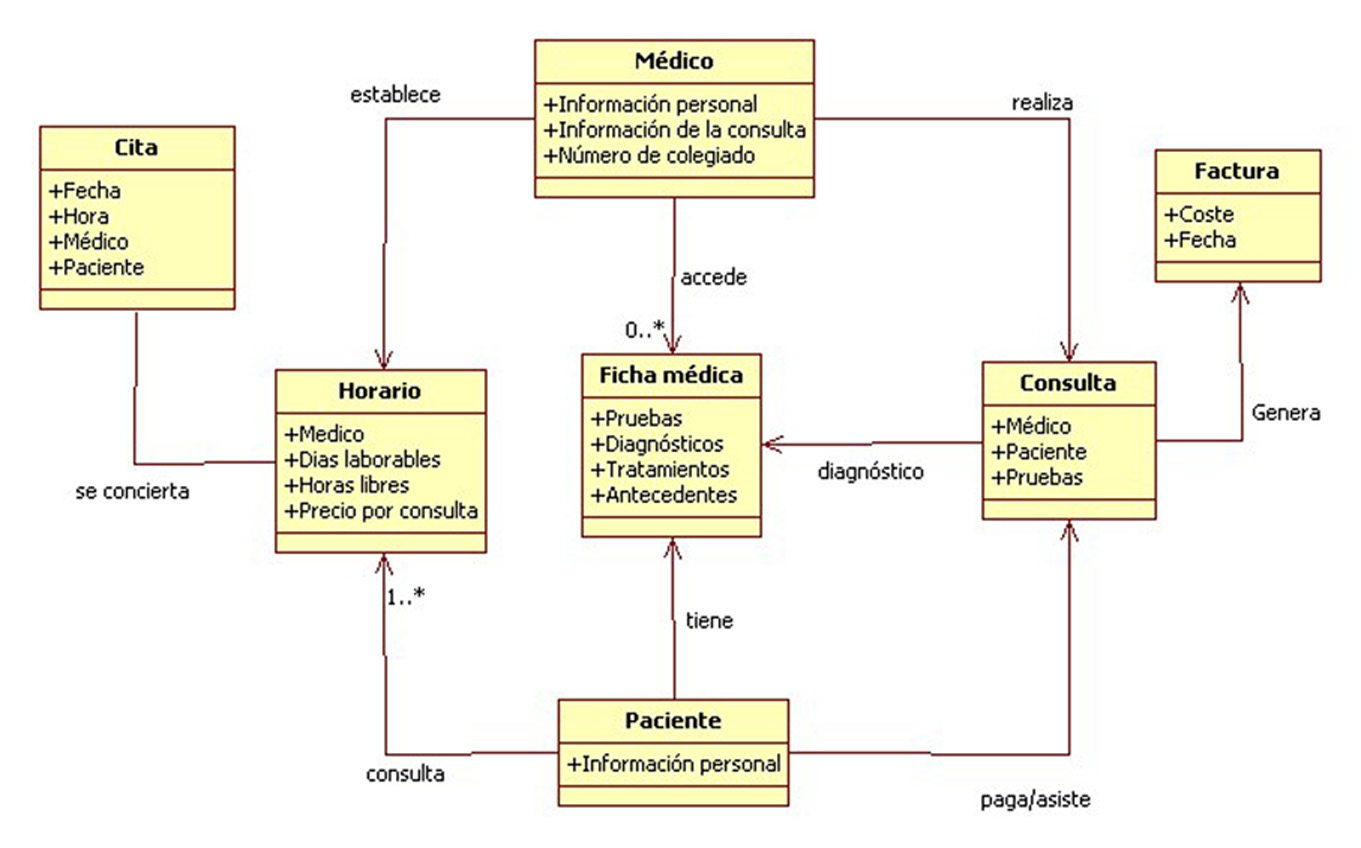
\includegraphics{img/modelo.jpg}
	  \caption{Modelo del dominio}
	  \label{modelodominio}
	\end{figure}

	\subsection{Glosario}
	Acorde a lo visto en la Figura \ref{modelodominio} vamos a establecer un pequeño glosario.

	\begin{itemize}
		\item \textbf{Cita.} Refleja que se concierta una consulta que supondrá el encuentro entre médico y paciente en la fecha y hora seleccionada. 
		\item \textbf{Consulta.} Encuentro entre médico y paciente.
		\item \textbf{Coste.} Transacción económica del importe de la consulta. 
		\item \textbf{Diagnóstico.} Calificación que da el médico a la enfermedad según los signos que advierte. Se añade a la ficha del paciente.
		\item \textbf{Factura.} Toda cita tiene un coste que debe ser abonado. Una vez realizado el pago, se genera una factura que corrobora que la transacción económica se ha producido.	
		\item \textbf{Ficha médica.} Información del paciente. Contiene tanto la información personal como todo tipo de información sanitaria: antecedentes, pruebas, diagnósticos, informes, tratamientos, etc.
		\item \textbf{Horario.} Horario del médico en el que aparece reflejado sus días laborables y sus horas disponibles, así como el coste de la consulta.
		\item \textbf{Médico.} Especialista encargado de la consulta con el paciente.
		\item \textbf{Paciente.} Persona con patología que acude a la consulta de un médico.
	\end{itemize}
% section modelo_del_dominio (end) % Modelo del dominio
		% ----------------------------------
% Casos de uso
% ----------------------------------
	
\section{Casos de uso} % (fold)
	\label{cha:casos_de_uso}

% 
% Sec Tipos de usuarios
%
\subsection{Introducción} % (fold)
	\label{sec:modelo_casos_de_uso}
	
		En esencia, un caso de uso narra una historia estilizada sobre cómo interactúa un usuario final (en esta aplicación, un médico, un paciente o un administrador) con el sistema en circunstancias específicas. La historia puede ser un texto narrativo, un lineamiento de tareas o interacciones, una descripción basada en un formato o una representación diagramática. Sin importar su forma, \textbf{un caso de uso ilustra el software o sistema desde el punto de vista del usuario final.}
		
		\medskip
		\fcolorbox{negro}{gris}{\parbox{15cm}{Los \textit{Casos de Uso} no son parte del diseño (cómo), sino parte del análisis (qué). De esta forma nos ayudan a describir qué es lo que es sistema debe hacer desde el punto de vista del usuario. Es decir, describen un uso del sistema y cómo éste interactúa con el usuario.}}
		
		\medskip		
		El primer paso para escribir un caso de uso es \textbf{definir un conjunto de <<actores>>} que estarán involucrados en la historia. Los \textit{actores} son las distintas personas (o dispositivos) que usan el sistema o producto en el contexto de la función y comportamiento que va a describirse. Los actores representan los papeles que desempeñan las personas (o dispositivos) cuando opera el sistema. Con una definición más formal, \textbf{un \textit{actor} es cualquier cosa que se comunique con el sistema o producto y que sea externo a éste.} Todo actor tiene uno o más objetivos cuando utiliza el sistema.
		
		 En este documento \textbf{nos centraremos en los diagramas UML y en la descripción formal de los casos de uso.} La representación con diagramas facilita la comprensión y cada caso de uso está representado por un óvalo. Por su parte, la descripción se hará de manera formal y como cualquier otra forma de descripción escrita, un caso de uso tiene sus limitaciones, y si la descripción es poco clara, el caso de uso será confuso o ambiguo. Por ello, se intentará mostrar un nivel de detalle y precisión significativos para que la comprensión sea la mejor posible.
		
	
	\subsection{Diagramas de casos de uso} % (fold)
	\label{sub:diagramas_de_casos_de_uso}
	
		Los diagramas de casos de uso que forman la aplicación están agrupados principalmente en seis paquetes.
		\begin{itemize}
			\item \textit{Actores}. Principales personas que se comunican con el sistema.
			\item \textit{Actividades Generales}. Agrupa las acciones que puede realizar cualquier usuario sin necesidad de estar registrado.
			\item \textit{Actividades de los médicos}. Todo lo referente a la funcionalidad que los usuarios con rol de médico esperan del sistema.
			\item \textit{Actividades de los pacientes}. Todas aquellas actividades que pueden realizar los usuarios registrados con el rol de paciente.
			\item \textit{Gestión de fichas médicas}. Abarca todas las acciones que pueden realizar los usuarios registrados, tanto médicos como pacientes, sobre las fichas médicas.
			\item \textit{Panel del Administrador}. Funcionalidades asociadas al Administrador del sistema.
		\end{itemize}
	
		\fbox{\parbox{15cm}{En el presente documento se especifican los diagramas y las descripciones formales de la gran mayoría de los casos de uso que definen la aplicación, dejando algunos sin definir debido a su gran simplicidad.}}
	
		\subsubsection{Actores} % (fold)
		\label{sec:actores}
			Podemos observar que existen tres tipos de actores principales (Figura \ref{fig:actores}), un usuario genérico, un administrador y un usuario registrado. De éste último heredan otros dos tipos de actores, los médicos y los pacientes.
			\begin{figure}[H]
			  \centering
			    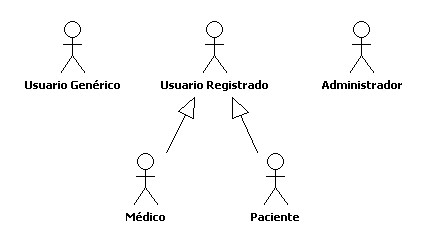
\includegraphics[width=10cm]{img/jpg/casos_uso/Actores.jpg}
			  \caption{Actores.}
			  \label{fig:actores}
			\end{figure}
			
			
		% section actores (end)
	
		\subsubsection{Actividades Generales} % (fold)
		\label{sec:actividades_generales}
		
			Las actividades generales son una serie de acciones que puede hacer un actor genérico del sistema, es decir, aquellos que no necesitan estar identificados en el sistema.
			\paragraph{Registro e información} % (fold)
			\label{par:registro_e_informacion}
				Un usuario genérico podrá registrarse como médico o como paciente. Anotar de antemano que una vez registrado, deberá rellenar su información personal, y opcionalmente, adjuntar una foto para su perfil. (Figura \ref{fig:reg_inf}). Además, si es médico, deberá rellenar la información de su consulta. Como se explicará más adelante en diseño, esto ocurre debido a que el formulario de registro únicamente incluye los campos de email, contraseña e idioma. Una vez el usuario ha accedido al sistema, le será menos pesado rellenar toda su información asociada.
				\begin{figure}[H]
				  \centering
				    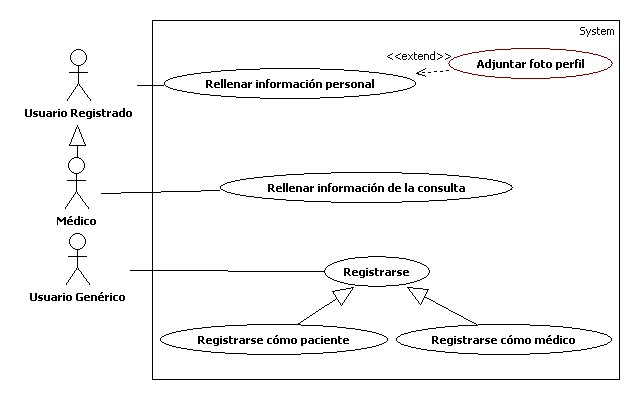
\includegraphics[width=14cm]{img/jpg/casos_uso/Registro_e_informacion.jpg}
				  \caption{Registro e información.}
				  \label{fig:reg_inf}
				\end{figure}
			% paragraph registro_e_información (end)
			
			\paragraph{Características generales} % (fold)
			\label{par:caracteristicas_generales}
				Las características generales (Figura \ref{fig:caracteristicas}) son una serie de acciones que puede realizar un actor genérico para ver diversa información de la aplicación o para interactuar con ella, en algunos casos.
							
			% paragraph características_generales (end)
		
			\paragraph{Acceso y Autentificación} % (fold)
			\label{par:acceso_y_autentificacion}
				Son funcionalidades que pueden realizar los actores registrados para iniciar o cerrar sesión (Figura \ref{fig:acceso}). Además, existe la posibilidad de no cerrar sesión. Otra función es la de recordar contraseña.
				\begin{figure}[H]
				  \centering
				    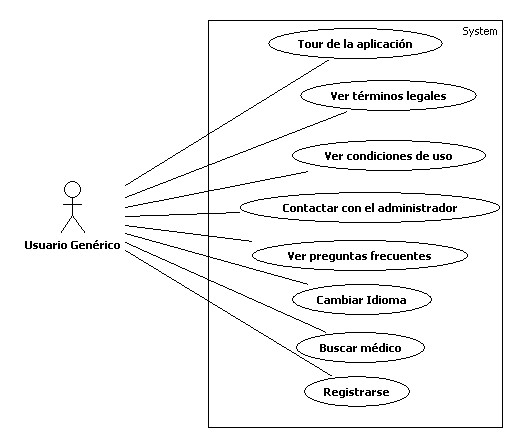
\includegraphics[width=12cm]{img/jpg/casos_uso/Generales.jpg}
				  \caption{Características Generales.}
				  \label{fig:caracteristicas}
				\end{figure}
				
				\begin{figure}[H]
				  \centering
				    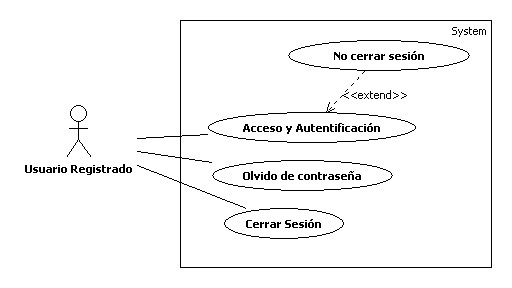
\includegraphics[width=12cm]{img/jpg/casos_uso/Acceso_y_Autentificacion.jpg}
				  \caption{Acceso y Autentificación.}
				  \label{fig:acceso}
				\end{figure}
			% paragraph acceso_y_autentificación (end)
			
		% section actividades_generales (end)
	
	
		\subsubsection{Actividades de los médicos} % (fold)
		\label{sec:actividades_de_los_medicos}
		
			Pretenden abordar todas las acciones que puede realizar un actor registrado identificado en el sistema con el rol de médico.
			\paragraph{Panel de Configuración de los médicos} % (fold)
			\label{par:panel_de_configuracion_de_los_medicos}
				Un médico tiene acceso a un panel de configuración (Figura \ref{fig:config_med}) desde el cual modificar los datos personales y de su consulta médica (Figura \ref{fig:config_med_datos}), modificar los datos de su cuenta (Figura \ref{fig:config_med_cuenta}), configurar su horario de disponibilidad, las notificaciones que recibirá en función de diversos sucesos y los motivos que incluirá a la hora de anotar ingresos y gastos.
				
				Respecto a los datos, cabe destacar que podrá adjuntar su propio curriculum, y una foto de su perfil. Respecto a la cuenta, que podrá cambiar su contraseña, su email, el idioma y darse de baja en el servicio cuando lo desee.
				
				Siempre que se modifiquen sus datos o la información de su cuenta, se almacenará la acción realizada en un historial del médico, que contendrá toda la información relevante de la que pueda ser interesante mantener un registro.
				\begin{figure}[H]
				  \centering
				    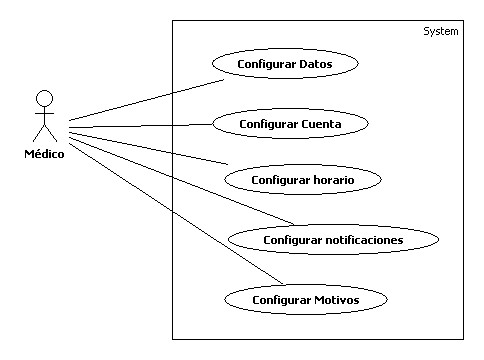
\includegraphics[width=12cm]{img/jpg/casos_uso/Configuracion_Medico.jpg}
				  \caption{Panel de configuración de los médicos.}
				  \label{fig:config_med}
				\end{figure}
				
				\begin{figure}[H]
				  \centering
				    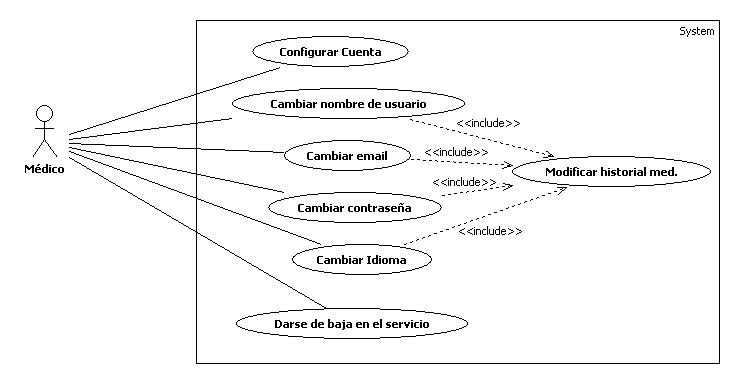
\includegraphics[width=15cm]{img/jpg/casos_uso/Configurar_Cuenta_Medico.jpg}
				  \caption{Configurar cuenta del médico.}
				  \label{fig:config_med_cuenta}
				\end{figure}
				
				\bigskip
				
				\begin{figure}[H]
				  \centering
				    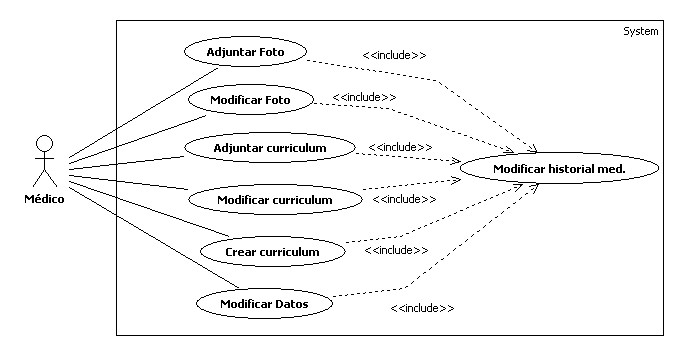
\includegraphics[width=15cm]{img/jpg/casos_uso/Configurar_Datos_Medico.jpg}
				  \caption{Configurar los datos del médico.}
				  \label{fig:config_med_datos}
				\end{figure}
			% paragraph panel_de_configuración_de_los_médicos (end)
		
			\bigskip
			\bigskip
			\paragraph{Gestión del Calendario del médico} % (fold)
			\label{par:gestion_del_calendario_del_medico}
			
				Un actor médico puede realizar una serie de acciones relacionadas con su calendario (Figura \ref{fig:cal_med}), entre ellas realizar la vista diaria, semanal o mensual de las citas que tiene concertadas. Desde ellas, podrá acceder a la vista de la ficha médica del paciente o anular una cita puntual (modificará el historial del médico y el del paciente). Por otro lado, debe configurar su horario de disponibilidad para que esté visible por los posibles pacientes potenciales y configurar las notificaciones que le llegarán al email. Por último, puede anular un día entero. La modificación de cualquiera de las tres últimas funcionalidades es relevante, y quedará registrada en el historial del médico.
				\begin{figure}[H]
				  \centering
				    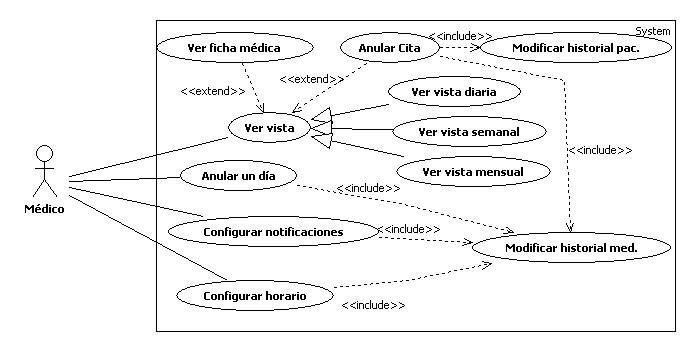
\includegraphics[width=14cm]{img/jpg/casos_uso/Gestion_calendario.jpg}
				  \caption{Gestión del Calendario del médico.}
				  \label{fig:cal_med}
				\end{figure}
			% paragraph gestión_del_calendario_del_médico (end)
		
			\paragraph{Gestión de pacientes} % (fold)
			\label{par:gestion_de_pacientes}
				Un actor médico puede ver una lista de todos sus pacientes o buscar pacientes en función de diversos filtros. Cuando haya encontrado al paciente deseado, podrá acceder a su ficha médica.
				\begin{figure}[H]
				  \centering
				    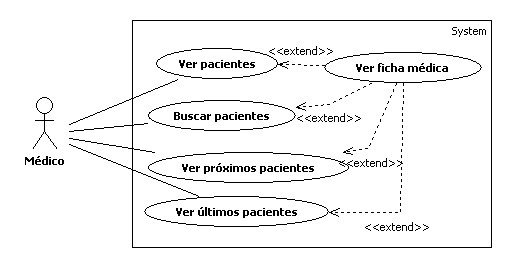
\includegraphics[width=10cm]{img/jpg/casos_uso/Gestion_Pacientes.jpg}
				  \caption{Gestión Pacientes del médico.}
				  \label{fig:pac_med}
				\end{figure}
			% paragraph gestión_de_pacientes (end)
		
			\paragraph{Gestión de estadísticas} % (fold)
			\label{par:gestion_de_estadisticas}
				Un actor médico puede ver una serie de estadísticas generales del último mes, del último año o de los últimos años (Figura \ref{fig:estad_med}). 
				
			% paragraph gestión_de_estadísticas (end)
			
			
			\paragraph{Administración y Gestión del Centro médico} % (fold)
			\label{par:administracion_y_gestion_del_centro_medico}
				
				(Figura \ref{fig:ad_ges_med}) Un médico puede anotar todos sus ingresos y sus gastos para ver un balance de la economía. También podrá buscar la factura que sea necesaria. Otra cosa que podrá administrar serán los votos recibidos por los distintos pacientes a los que ya haya visitado. Por último, podrá acceder al historial y realizar búsquedas mediante distintos filtros de toda la información relevante resultado de alguna acción de la aplicación. Lo relacionado a añadir ingresos o gastos actualizará el historial del médico. Además, siempre que se anote un ingreso, se generará una factura asociada.
				
				\begin{figure}[H]
				  \centering
				    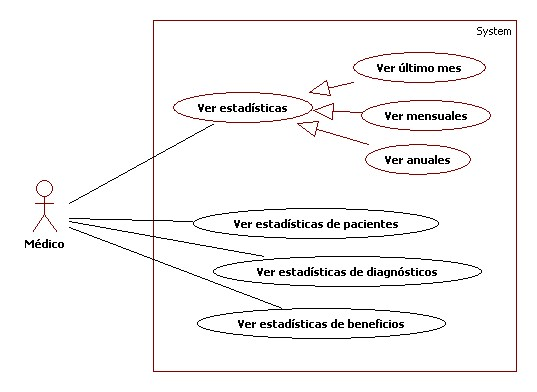
\includegraphics[width=12cm]{img/jpg/casos_uso/Estadisticas.jpg}
				  \caption{Gestión de Estadísticas de los médicos.}
				  \label{fig:estad_med}
				\end{figure}
				
				\begin{figure}[H]
				  \centering
				    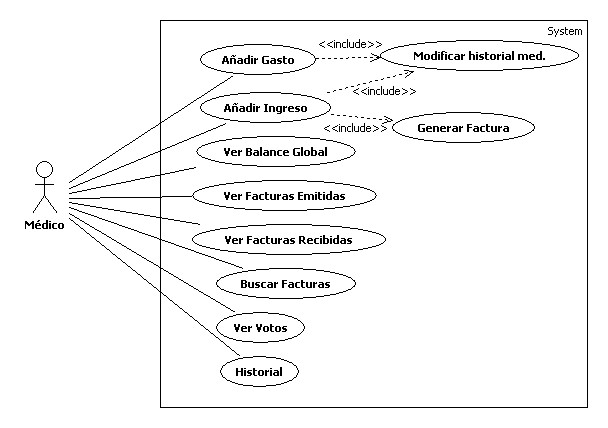
\includegraphics[width=14cm]{img/jpg/casos_uso/Administracion_y_Gestion.jpg}
				  \caption{Administración y Gestión del centro médico.}
				  \label{fig:ad_ges_med}
				\end{figure}
			% paragraph administración_y_gestión_del_centro_médico (end)
					
		% section actividades_de_los_médicos (end)
	
		\subsubsection{Actividades de los pacientes} % (fold)
		\label{sec:actividades_de_los_pacientes}
		Pretenden abordar todas las acciones que puede realizar un actor registrado identificado en el sistema con el rol de paciente.
			\paragraph{Calendario del Paciente} % (fold)
			\label{par:calendario_del_paciente}
				Un actor paciente puede realizar una serie de acciones relacionadas con su calendario (Figura \ref{fig:cal_pac}), entre ellas realizar la vista diaria, semanal o mensual de las citas que tiene concertadas. Desde ellas, podrá acceder a la información del médico o anular una cita puntual. Por otro lado, debe configurar las notificaciones que le llegarán al email. Siempre que anule una cita o que modifique la configuración de sus notificaciones, se registrarán los cambios en el historial del paciente.
				\begin{figure}[H]
				  \centering
				    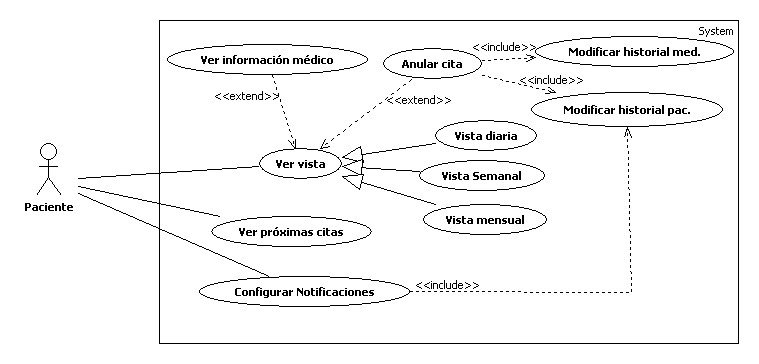
\includegraphics[width=14cm]{img/jpg/casos_uso/Calendario_del_paciente.jpg}
				  \caption{Calendario del Paciente.}
				  \label{fig:cal_pac}
				\end{figure}
			% paragraph calendario_del_paciente (end)
		
			\paragraph{Gestión de médicos del paciente} % (fold)
			\label{par:gestion_de_medicos_del_paciente}
			
				(Figura \ref{fig:med_pac}) Un actor paciente puede ver una lista con todos sus médicos o buscarlos según diversos filtros. Posee una serie de especialistas asignados a una lista de favoritos, para poder acceder a ellos más rápidamente. Una vez encontrado el médico deseado, podrá ver su horario y asignarse una cita, ver su información y añadirlo a sus favoritos. Lo relacionado a asignarse una cita, añadir médico favorito o votar médico quedará registrado en el historial del paciente por considerarse acciones relevantes.
				
			% paragraph gestión_de_médicos_del_paciente (end)
			
			\paragraph{Ficha médica} % (fold)
			\label{par:ficha_medica}
				
				Un paciente siempre podrá acceder a ver su ficha médica (Figura \ref{fig:ficha_pac}). Todas las actividades relacionadas con la ficha médica se tratan en el siguiente apartado (Gestión de fichas médicas).
				\begin{figure}[H]
				  \centering
				    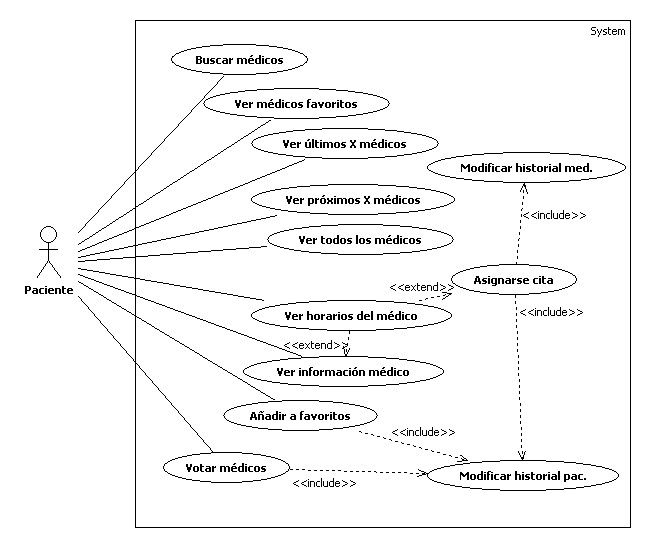
\includegraphics[width=14cm]{img/jpg/casos_uso/Gestion_medicos.jpg}
				  \caption{Gestión de médicos del paciente.}
				  \label{fig:med_pac}
				\end{figure}
				
				\begin{figure}[H]
				  \centering
				    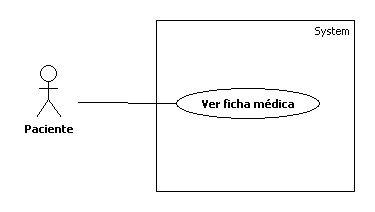
\includegraphics[width=10cm]{img/jpg/casos_uso/Ver_ficha_medica.jpg}
				  \caption{Ver ficha médica del paciente.}
				  \label{fig:ficha_pac}
				\end{figure}
			% paragraph ficha_médica (end)
			
			\paragraph{Panel de configuración del paciente} % (fold)
			\label{par:panel_de_configuracion_del_paciente}
				Un paciente tiene acceso a un panel de configuración (Figura \ref{fig:config_pac}) desde el cual modificar los datos personales (Figura \ref{fig:datos_pac}), modificar los datos de su cuenta (Figura \ref{fig:cuenta_pac}) y establecer las notificaciones que recibirá en función de diversos sucesos. Respecto a los datos, cabe destacar que podrá adjuntar o modificar una foto de su perfil. Respecto a la cuenta, que podrá cambiar su contraseña, su email, el idioma y darse de baja en el servicio cuando lo desee.
				
				Siempre que se modifiquen sus datos o la información de su cuenta, se almacerá la acción realizada en un historial del paciente, que contendrá toda la información relevante de la que pueda ser interesante mantener un registro.
				
				\begin{figure}[H]
				  \centering
				    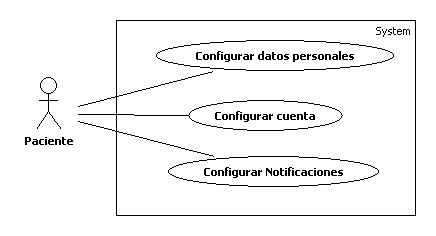
\includegraphics[width=10cm]{img/jpg/casos_uso/Configuracion_pacientes.jpg}
				  \caption{Panel de configuración del paciente.}
				  \label{fig:config_pac}
				\end{figure}
				
				\begin{figure}[H]
				  \centering
				    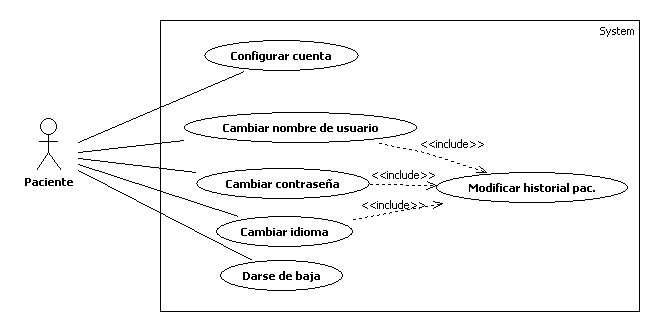
\includegraphics[width=14cm]{img/jpg/casos_uso/Cuenta.jpg}
				  \caption{Configuración de cuenta del paciente.}
				  \label{fig:cuenta_pac}
				\end{figure}
				
				\begin{figure}[H]
				  \centering
				    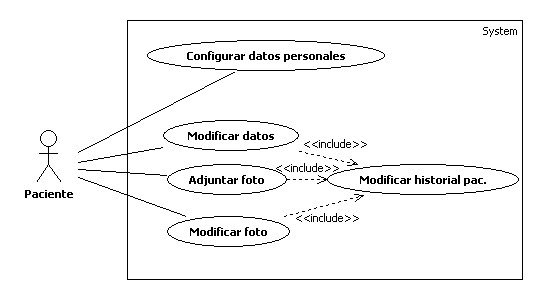
\includegraphics[width=12cm]{img/jpg/casos_uso/Datos.jpg}
				  \caption{Configuración de datos del paciente.}
				  \label{fig:datos_pac}
				\end{figure}
			% paragraph panel_de_configuración_del_paciente (end)
			
		
		% section actividades_de_los_pacientes (end)
	
		\subsubsection{Gestión de fichas médicas} % (fold)
		\label{sec:gestion_de_fichas_medicas}
			
			Los diagramas pretenden abarcar todo lo que un usuario registrado, tanto médico como paciente, podrá realizar con las fichas médicas.
			\paragraph{Información Personal} % (fold)
			\label{par:informacion_personal}
				Se muestra la información personal del paciente (Figura \ref{fig:infpers_fic}). Se podrán modificar los datos y adjuntar o modificar la foto del perfil.
				\begin{figure}[H]
				  \centering
				    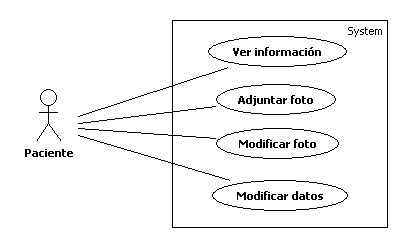
\includegraphics[width=11cm]{img/jpg/casos_uso/Informacion_personal.jpg}
				  \caption{Ficha médica. Información Personal.}
				  \label{fig:infpers_fic}
				\end{figure}
			% paragraph información_personal (end)
		
			\paragraph{Antecedentes} % (fold)
			\label{par:antecedentes}
				(Figura \ref{fig:ant_fic}) Los antecedentes de un paciente pueden ser de tres tipos, \textit{fisiológicos, familiares o personales}. Se podrán añadir o modificar antecedentes (quedará registrado en el historial de la ficha médica). También se puede imprimir y exportar.
				\begin{figure}[H]
				  \centering
				    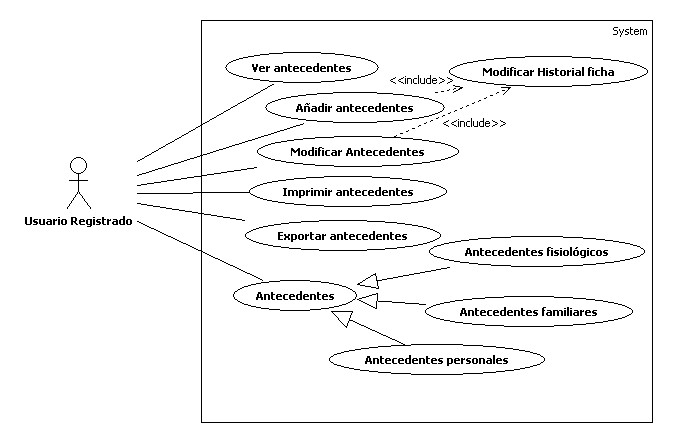
\includegraphics[width=14cm]{img/jpg/casos_uso/Antecedentes.jpg}
				  \caption{Ficha médica. Antecedentes.}
				  \label{fig:ant_fic}
				\end{figure}
			% paragraph antecedentes (end)
			
			\paragraph{Exploración} % (fold)
			\label{par:exploracion}
				(Figura \ref{fig:exp_fic}) Siempre que se añada o se modifique una exploración se modificará el historial de la ficha médica.
				\begin{figure}[H]
				  \centering
				    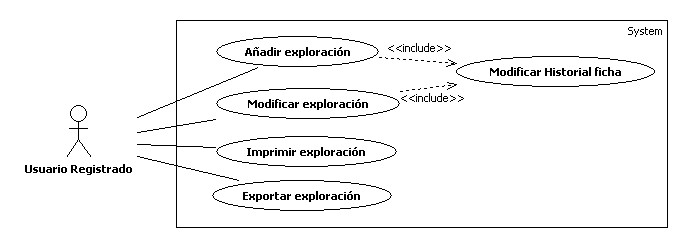
\includegraphics[width=14cm]{img/jpg/casos_uso/Exploracion.jpg}
				  \caption{Ficha médica. Exploración}
				  \label{fig:exp_fic}
				\end{figure}
			% paragraph exploración (end)
			
			\paragraph{Diagnósticos} % (fold)
				(Figura \ref{fig:diag_fic}) Cuando se añada o se modifique un diagnóstico, se modificará el historial de la ficha. Se podrá ver una lista con todos los diagnósticos y ver cada uno de ellos de manera más detallada(el último se ve así por defecto). Podrán imprimirse y exportarse.
			\label{par:diagnosticos}
				\begin{figure}[H]
				  \centering
				    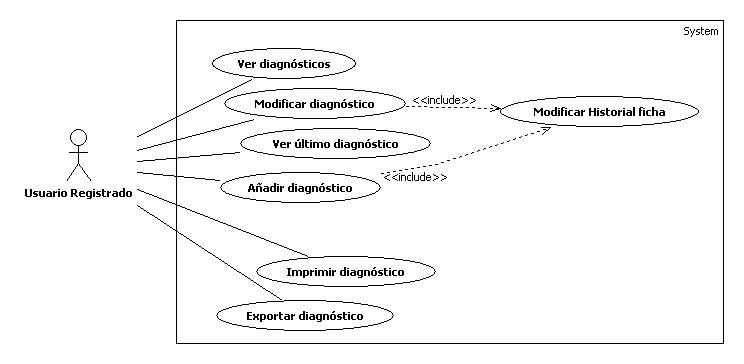
\includegraphics[width=14cm]{img/jpg/casos_uso/Diagnosticos.jpg}
				  \caption{Ficha médica. Diagnóstico.}
				  \label{fig:diag_fic}
				\end{figure}
			% paragraph diagnósticos (end)
			
			\paragraph{Tratamientos} % (fold)
			\label{par:tratamientos}
			(Figura \ref{fig:trat_fic}) Siempre que se añada o se modifique un tratamiento, se modificará el historial de la ficha médica. Se podrá ver una lista con todos los tratamientos anteriores y de forma más específica el tratamiento actual. Podrán imprimirse y exportarse.
				\begin{figure}[H]
				  \centering
				    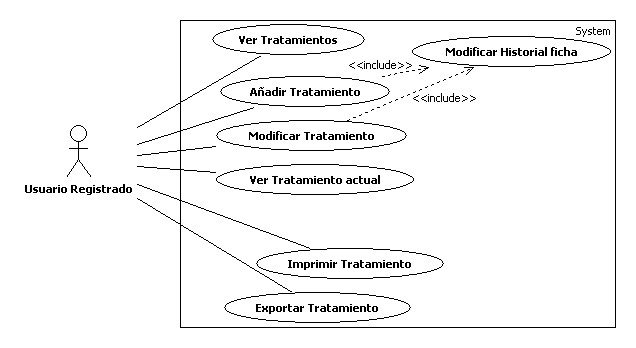
\includegraphics[width=13cm]{img/jpg/casos_uso/Tratamientos.jpg}
				  \caption{Ficha médica. Tratamiento.}
				  \label{fig:trat_fic}
				\end{figure}
			% paragraph tratamientos (end)
			
			\paragraph{Informes} % (fold)
			\label{par:informes}
				(Figura \ref{fig:inf_fic}) Siempre que se añada o se modifique un informe, se modificará el historial de la ficha médica. Se podrá ver una lista con todos los informes y ver cada uno de ellos de manera más detallada(el último se ve así por defecto). Podrán imprimirse y exportarse.
				\begin{figure}[H]
				  \centering
				    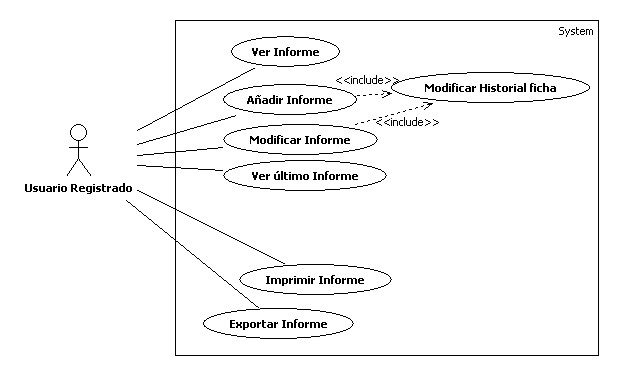
\includegraphics[width=14cm]{img/jpg/casos_uso/Informes.jpg}
				  \caption{Ficha médica. Informes.}
				  \label{fig:inf_fic}
				\end{figure}
			% paragraph informes (end)
			
			\paragraph{Observaciones} % (fold)
			\label{par:observaciones}
				(Figura \ref{fig:obs_fic}) Sólo accesible por el médico. Permite a éste ver, añadir o modificar las observaciones sobre un paciente. Las dos últimas funcionalidades modificarán, además, el historial de la ficha médica.
				\begin{figure}[H]
				  \centering
				    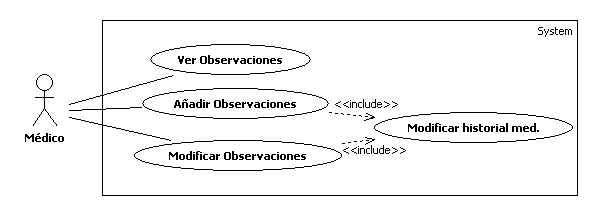
\includegraphics[width=14cm]{img/jpg/casos_uso/Observaciones.jpg}
				  \caption{Ficha médica. Observaciones.}
				  \label{fig:obs_fic}
				\end{figure}
			% paragraph observaciones (end)
			
			\paragraph{Historial de la ficha} % (fold)
			\label{par:historial_de_la_ficha}
				En el historial de la ficha médica se almacena toda la información que pueda resultar relevante cada vez que una acción en la aplicación realice una función sobre la información que contiene. Además, éstas acciones en las que se añada o modifique información importante, también quedarán registradas en la ficha del médico y en la ficha del paciente. Se podrán realizar búsquedas mediante diversos filtros en el historial de las fichas. Podrá imprimirse y exportarse. (Figura \ref{fig:hist_fic}).
				\begin{figure}[H]
				  \centering
				    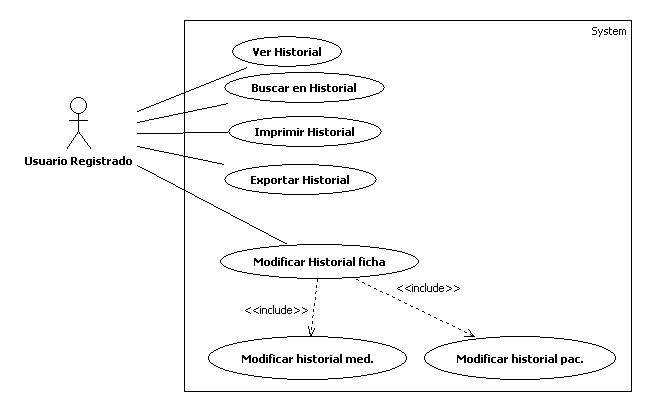
\includegraphics[width=14cm]{img/jpg/casos_uso/Historial_ficha.jpg}
				  \caption{Ficha médica. Historial de la Ficha.}
				  \label{fig:hist_fic}
				\end{figure}
			% paragraph historial_de_la_ficha (end)
			
			\paragraph{Pruebas} % (fold
			
				(Figura \ref{fig:pruebas_gestion_fic}) Se podrán ver pruebas y añadirlas (al insertar una nueva prueba en la aplicación, se modifica el historial de la ficha médica). El actor médico es el único que puede solicitar una nueva prueba. Podrán imprimirse y exportarse.
				
				Se pueden ver distintos tipos de pruebas (Figura \ref{fig:pruebas_ver_fic}) relacionadas con cada una de las posibles especialidades. Lo mismo ocurre con la opción de añadir pruebas (Figura \ref{fig:pruebas_add_fic}) y de solicitar pruebas (Figura \ref{fig:pruebas_sol_fic}). Sin embargo, esta última acción sólo podrán realizarla los actores médicos.
				
			\fbox{\parbox{15cm}{La aplicación se centrará sólo en las pruebas de analíticas, radiodiagnósticos, anatomía patológica y electromiografías. Se pueden añadir modularmente las opciones para otro tipo de pruebas específicas de cada especialidad.}}	
				
			\label{par:pruebas}
				\begin{figure}[H]
				  \centering
				    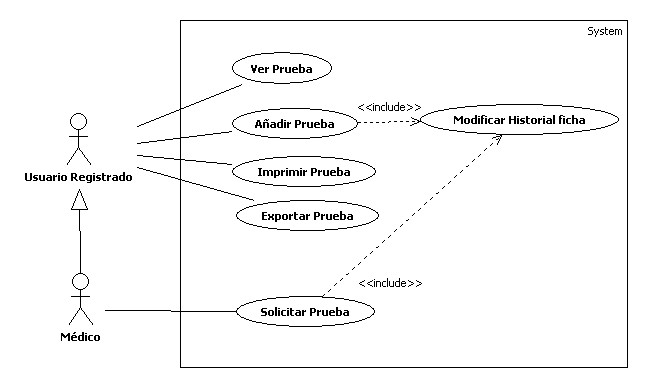
\includegraphics[width=13cm]{img/jpg/casos_uso/Gestion_pruebas.jpg}
				  \caption{Ficha médica. Pruebas. Gestión de Pruebas.}
				  \label{fig:pruebas_gestion_fic}
				\end{figure}
				
				\begin{figure}[H]
				  \centering
				    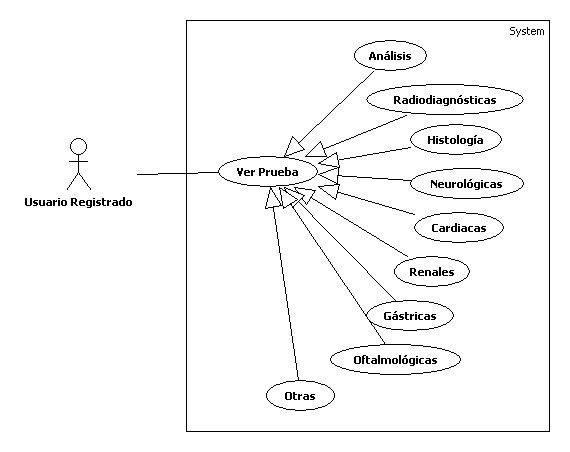
\includegraphics[width=10cm]{img/jpg/casos_uso/Ver_Prueba.jpg}
				  \caption{Ficha médica. Pruebas. Ver Prueba.}
				  \label{fig:pruebas_ver_fic}
				\end{figure}
				
				\begin{figure}[H]
				  \centering
				    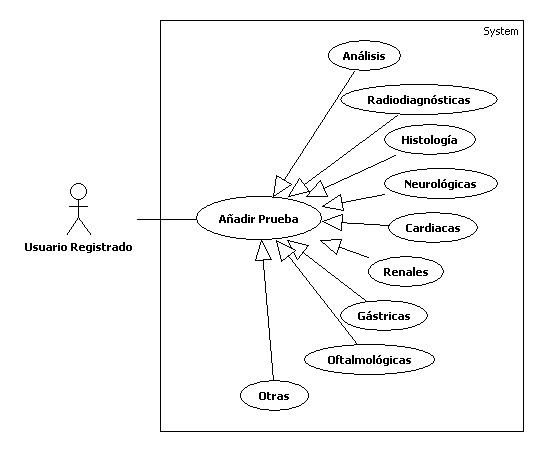
\includegraphics[width=10cm]{img/jpg/casos_uso/Add_Prueba.jpg}
				  \caption{Ficha médica. Pruebas. Añadir Prueba.}
				  \label{fig:pruebas_add_fic}
				\end{figure}
				
				\begin{figure}[H]
				  \centering
				    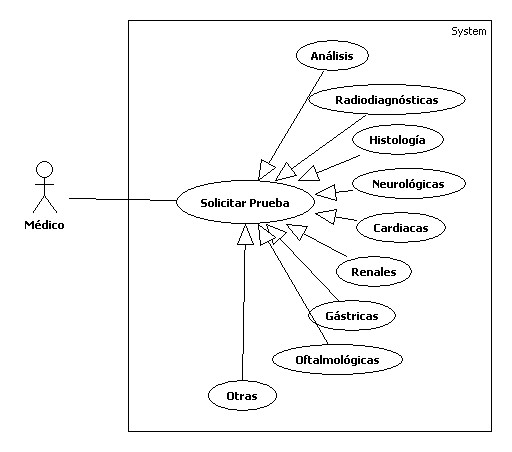
\includegraphics[width=10cm]{img/jpg/casos_uso/Solicitar_Prueba.jpg}
				  \caption{Ficha médica. Pruebas. Solicitar prueba.}
				  \label{fig:pruebas_sol_fic}
				\end{figure}
			% paragraph pruebas (end)
			
		% section gestión_de_fichas_médicas (end)
	
		\subsubsection{Panel del Administrador} % (fold)
		\label{sec:panel_del_administrador}
		
			El actor Administrador del sistema tiene una serie de funciones importantes relativas a la aplicación. 
			
			Entre ellas cabe destacar la de \textit{verificar médicos}, con la cuál da de alta a un médico en el sistema haciéndolo visible para el resto de usuarios de la aplicación. Operaciones similares son las de \textit{eliminar médicos, suspender médicos o reactivar médicos}. 
			
			Otras funciones son las de \textit{ver, contestar y eliminar} las preguntas de los usuarios. También podrá modificar fácilmente \textit{las condiciones de uso, los datos de contacto y los términos legales}. 
			
			Por último, podrá \textit{agregar a otro administrador}.
			
			\begin{figure}[H]
			  \centering
			    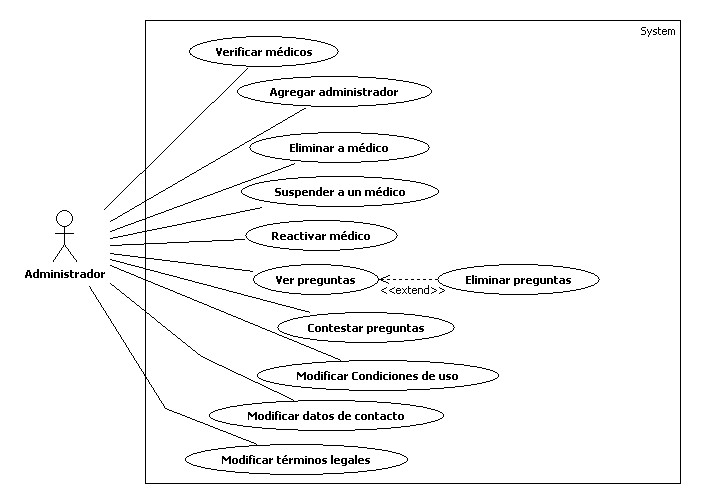
\includegraphics[width=15cm]{img/jpg/casos_uso/Panel_de_Administrador.jpg}
			  \caption{Panel del Administrador.}
			  \label{fig:panel_admin}
			\end{figure}
					
		% section panel_del_administrador (end)
	
	% subsubsection diagramas_de_casos_de_uso (end)
	\newpage
	\subsection{Descripción formal de los Casos de Uso} % (fold)
	\label{sub:descripcion_formal_de_los_casos_de_uso}
		
		La especificación de un caso de uso debe describir el modo en que un actor interactúa con el sistema. Es mucho más importante que los diagramas, de hecho, el 90 por ciento del contenido de los casos de uso está en dichas descripciones.
			
		\subsubsection{Estructura de la descripción} % (fold)
		\label{sub:estructura_de_la_descripcion}
		
			Para realizar la descripción formal de los casos de uso se van a utilizar unas tablas en las que se pretende abarcar toda la información necesaria para realizar dicha tarea. Los campos empleados serán los siguientes.
		
			\begin{itemize}
				\item \textbf{Identificador}. Cada caso de uso tendrá un ID único. La estructura será \textit{Categoría} + Número del caso de uso. Las categorías se agrupan de forma jerárquica en seis grandes grupos.
					\begin{itemize}
						\item \textit{ACT}. Actores.
						\item \textit{GAG}. Gestión de Actividades generales.
						\item \textit{GAM}. Gestión de Actividades de los médicos.
						\item \textit{GAP}. Gestión de Actividades de los pacientes.
						\item \textit{GFM}. Gestión de las Fichas médicas.
						\item \textit{GPA}. Gestión del Panel del Administrador.
					\end{itemize}
				
				\item \textbf{Nombre}. Todo caso de uso tendrá un nombre que refleja las tareas y funcionalidades que el usuario podrá llevar a cabo. Suele estar formado por un verbo que ejecute una acción y un sustantivo.

				\item \textbf{Historial}. Tiene los siguientes apartados.
					\begin{itemize}
						\item \textit{Fecha de creación}. Fecha en la que se documentó el caso de uso.
						\item \textit{Fecha de la última actualización}. Fecha en la que se realizó la última modificación en la descripción del caso de uso.
					\end{itemize}
					
				\item \textbf{Actores}. El nombre del actor que inició este caso de uso y cualquier otro actor que participe en su realización.  
			
				\item \textbf{Descripción}. Proporciona una breve descripción del caso de uso.
				
				\item \textbf{Precondición}. Describe lo que se sabe que es verdadero antes de que inicie el caso de uso. 
				
				\item \textbf{Postcondición}. Describe el estado del sistema al finalizar la ejecución del caso de uso.
				
				\item \textbf{Camino normal}. Proporcionar una descripción detallada de las acciones del usuario y las respuestas del sistema que se llevarán a cabo durante la ejecución del caso de uso en condiciones normales, es decir, si todo sucede como se esperaba. Esta secuencia de diálogo pretende alcanzar, en última instancia, el objetivo expuesto en el nombre y la descripción de casos de uso. Se hará mediante una lista numerada de las acciones realizadas por el actor, alternando con las respuestas proporcionadas por el sistema.
				
				\item \textbf{Camino alternativo}. Es un flujo alternativo al del camino normal, con diferencias en la secuencia de pasos que tienen lugar. 
				
				\item \textbf{Include}. Lista de otros casos de uso que se incluyen en éste. Funcionalidad común que aparece en múltiples casos de uso.
				
				\item \textbf{Extends}. Extensión de un caso de uso ya existente.
				
				\item \textbf{Iteración}. Indica si el caso de uso es prioritario (se realizará en la primera iteración) o no (se irán añadiendo cuando esté la estructura base funcionando).
		
			\end{itemize}
		
		% subsubsection estructura_de_la_descripción (end)
		
		\subsubsection{Descripción de los casos de uso} % (fold)
		\label{sub:descripcion_de_los_casos_de_uso}
		
			\paragraph{Actores} % (fold)
			\label{sub:actores}
				Encontramos cinco tipos de actores.
				\begin{itemize}
					\item \textit{Usuario Genérico}. Un usuario genérico es aquel que puede acceder a secciones del servicio para las que no es necesario estar registrado, como por ejemplo, ver preguntas frecuentes, realizar un tour por la aplicación o ver si algún médico está en el sistema. Podrá darse de alta en cualquier momento que lo desee, tanto con el rol de médico cómo con el de paciente.
					\item \textit{Usuario Registrado}. Puede ser un médico o un paciente. A ellos está destinada la aplicación.
						\begin{itemize}
							\item \textit{Médico}. Un usuario médico es aquel que se ha identificado cómo tal. Realizará funciones propias de los médicos. La aplicación está destinada a ellos principalmente.
							\item \textit{Paciente}. Un usuario paciente es aquel que accede a la aplicación en busca de un médico. Sus funcionalidades están más limitadas.
						\end{itemize}
					\item \textit{Usuario Administrador}. Un usuario Administrador gestionará temas concernientes a la aplicación. Será el que se encargue de dar de alta a los médicos que contraten el servicio, de contestar a las preguntas de los usuarios, etcétera. No utilizará ninguna funcionalidad de las destinadas a médicos y pacientes.
					 
				\end{itemize}
			% paragraph actores (end)
			\newpage
			\paragraph{Actividades Generales (GAG)} % (fold)
			\label{sub:actividades_generales_gag_}
			
				Una serie de acciones y funciones que pueden desarrollar los usuarios sin necesidad de estar registrados en el sistema. Además, lo referente al acceso y la autentificación por parte de usuarios registrados.
				\bigskip
			
				
				% Registrarse
				\begin{tabular}{|l|p{4cm}|p{4cm}|p{4cm}|}\hline
					\multicolumn{1}{|>{\columncolor{gris2}}l|}{Identificador} & \multicolumn{3}{|p{12cm}|}{GAG-01 (Figura \ref{fig:reg_inf})}	\\\hline
					\multicolumn{1}{|>{\columncolor{gris2}}l|}{Nombre} & \multicolumn{3}{|p{12cm}|}{Registrarse} \\\hline
					\multicolumn{1}{|>{\columncolor{gris2}}l|}{Fecha de creación} & 05/04/2011 & \multicolumn{1}{|>{\columncolor{gris2}}l|}{Fecha de actualización} & 24/08/2011 \\\hline
					\multicolumn{1}{|>{\columncolor{gris2}}l|}{Actor}  & \multicolumn{3}{|p{12cm}|}{Usuario Genérico} 	\\\hline			
					\multicolumn{4}{|>{\columncolor{gris2}}l|}{Descripción} \\\hline
					\multicolumn{4}{|p{16cm}|}{Un usuario genérico puede registrarse en el sistema. Cuando se registra, debe introducir su email y su contraseña. Puede registrarse con el rol de médico o con el de paciente. En función del tipo de rol que vaya a desempeñar, en futuros pasos, el usuario que se registre deberá rellenar distinta información.}	\\\hline
					\multicolumn{1}{|>{\columncolor{gris2}}l|}{Precondición} & \multicolumn{3}{|p{12cm}|}{Que el usuario genérico esté en la página de registro.} \\\hline
					\multicolumn{4}{|>{\columncolor{gris2}}l|}{Camino normal} \\\hline
					\multicolumn{4}{|p{16cm}|}{Caso de uso abstracto}	\\\hline
					\multicolumn{4}{|>{\columncolor{gris2}}l|}{Camino alternativo} \\\hline
					\multicolumn{4}{|p{16cm}|}{---}	\\\hline
					\multicolumn{1}{|>{\columncolor{gris2}}l|}{Postcondición} & \multicolumn{3}{|p{12cm}|}{Se guardan los datos en la base de datos y el usuario puede ingresar al sistema.}  \\\hline
					\multicolumn{1}{|>{\columncolor{gris2}}l|}{Include} & \multicolumn{3}{|p{12cm}|}{---}  \\\hline
					\multicolumn{1}{|>{\columncolor{gris2}}l|}{Extend} & \multicolumn{3}{|p{12cm}|}{---}  \\\hline
					\multicolumn{1}{|>{\columncolor{gris2}}l|}{Iteración} & \multicolumn{3}{|p{12cm}|}{Primera}  \\\hline			
				\end{tabular}  \bigskip \bigskip
				
				% Registrarse como paciente
				\begin{tabular}{|l|p{4cm}|p{4cm}|p{4cm}|}\hline
					\multicolumn{1}{|>{\columncolor{gris2}}l|}{Identificador} & \multicolumn{3}{|p{12cm}|}{GAG-02 (Figura \ref{fig:reg_inf})}	\\\hline
					\multicolumn{1}{|>{\columncolor{gris2}}l|}{Nombre} & \multicolumn{3}{|p{12cm}|}{Registrarse cómo paciente} \\\hline
					\multicolumn{1}{|>{\columncolor{gris2}}l|}{Fecha de creación} & 05/04/2011 & \multicolumn{1}{|>{\columncolor{gris2}}l|}{Fecha de actualización} & 24/08/2011 \\\hline
					\multicolumn{1}{|>{\columncolor{gris2}}l|}{Actor}  & \multicolumn{3}{|p{12cm}|}{Usuario Genérico} 	\\\hline			
					\multicolumn{4}{|>{\columncolor{gris2}}l|}{Descripción} \\\hline
					\multicolumn{4}{|p{16cm}|}{Un usuario puede registrarse como paciente.}	\\\hline
					\multicolumn{1}{|>{\columncolor{gris2}}l|}{Precondición} & \multicolumn{3}{|p{12cm}|}{Que el usuario esté en la página de registro de pacientes.} \\\hline
					
					\multicolumn{4}{|>{\columncolor{gris2}}l|}{Camino normal} \\\hline
						\multicolumn{4}{|p{16cm}|}{1.- Hacer click en Registrar como paciente.} \\
						\multicolumn{4}{|p{16cm}|}{2.- Ingresar el email.} \\
						\multicolumn{4}{|p{16cm}|}{3.- El software valida que el email sea válido.} \\
						\multicolumn{4}{|p{16cm}|}{4.- Ingresar contraseña} \\
						\multicolumn{4}{|p{16cm}|}{5.- Confirmar contraseña.} \\
						\multicolumn{4}{|p{16cm}|}{6.- El software valida que la contraseña coincide y que es fuerte.} \\
						\multicolumn{4}{|p{16cm}|}{7.- Darle al botón de aceptar.} \\
						\multicolumn{4}{|p{16cm}|}{8.- El software permite que el usuario se registre.} \\
						\multicolumn{4}{|p{16cm}|}{9.- El paciente puede ingresar.} \\\hline
					
					\multicolumn{4}{|>{\columncolor{gris2}}l|}{Camino alternativo} \\\hline
						\multicolumn{4}{|p{16cm}|}{3.1.- El software muestra un mensaje de error si el email no es válido.} \\
						\multicolumn{4}{|p{16cm}|}{6.1.- El software muestra un mensaje de error si la contraseña no coincide o es débil.} \\\hline

					\multicolumn{1}{|>{\columncolor{gris2}}l|}{Postcondición} & \multicolumn{3}{|p{12cm}|}{Se guardan los datos en la base de datos, el paciente inicia sesión y puede ingresar al sistema de ahora en adelante.}  \\\hline
					\multicolumn{1}{|>{\columncolor{gris2}}l|}{Include} & \multicolumn{3}{|p{12cm}|}{---}  \\\hline
					\multicolumn{1}{|>{\columncolor{gris2}}l|}{Extend} & \multicolumn{3}{|p{12cm}|}{---}  \\\hline
					\multicolumn{1}{|>{\columncolor{gris2}}l|}{Iteración} & \multicolumn{3}{|p{12cm}|}{Primera}  \\\hline			
				\end{tabular}  \bigskip \bigskip
				
				% Registrarse como médico
				\begin{tabular}{|l|p{4cm}|p{4cm}|p{4cm}|}\hline
					\multicolumn{1}{|>{\columncolor{gris2}}l|}{Identificador} & \multicolumn{3}{|p{12cm}|}{GAG-03 (Figura \ref{fig:reg_inf})}	\\\hline
					\multicolumn{1}{|>{\columncolor{gris2}}l|}{Nombre} & \multicolumn{3}{|p{12cm}|}{Registrarse cómo médico} \\\hline
					\multicolumn{1}{|>{\columncolor{gris2}}l|}{Fecha de creación} & 05/04/2011 & \multicolumn{1}{|>{\columncolor{gris2}}l|}{Fecha de actualización} & 11/04/2011 \\\hline
					\multicolumn{1}{|>{\columncolor{gris2}}l|}{Actor}  & \multicolumn{3}{|p{12cm}|}{Usuario Genérico} 	\\\hline			
					\multicolumn{4}{|>{\columncolor{gris2}}l|}{Descripción} \\\hline
					\multicolumn{4}{|p{16cm}|}{Un usuario puede registrarse cómo médico.}	\\\hline
					\multicolumn{1}{|>{\columncolor{gris2}}l|}{Precondición} & \multicolumn{3}{|p{12cm}|}{Que el usuario esté en la página de registro de médicos.} \\\hline
					\multicolumn{4}{|>{\columncolor{gris2}}l|}{Camino normal} \\\hline
						\multicolumn{4}{|p{16cm}|}{1.- Hacer click en Registrar como médico.} \\
						\multicolumn{4}{|p{16cm}|}{2.- Ingresar el email.} \\
						\multicolumn{4}{|p{16cm}|}{3.- El software valida que el email sea válido.} \\
						\multicolumn{4}{|p{16cm}|}{4.- Ingresar contraseña} \\
						\multicolumn{4}{|p{16cm}|}{5.- Confirmar contraseña.} \\						
						\multicolumn{4}{|p{16cm}|}{6.- El software valida que la contraseña coincide y que es fuerte.} \\
						\multicolumn{4}{|p{16cm}|}{7.- Darle al botón de aceptar.} \\
						\multicolumn{4}{|p{16cm}|}{8.- El software permite que el usuario se registre.} \\
						\multicolumn{4}{|p{16cm}|}{9.- El médico puede ingresar.} \\\hline
					
					\multicolumn{4}{|>{\columncolor{gris2}}l|}{Camino alternativo} \\\hline
						\multicolumn{4}{|p{16cm}|}{3.1.- El software muestra un mensaje de error si el email no es válido.} \\
						\multicolumn{4}{|p{16cm}|}{6.1.- El software muestra un mensaje de error si la contraseña no coincide o es débil.} \\\hline

					\multicolumn{1}{|>{\columncolor{gris2}}l|}{Postcondición} & \multicolumn{3}{|p{12cm}|}{Se guardan los datos en la base de datos, el médico inicia sesión y puede ingresar al sistema de ahora en adelante.}  \\\hline
					\multicolumn{1}{|>{\columncolor{gris2}}l|}{Include} & \multicolumn{3}{|p{12cm}|}{---}  \\\hline
					\multicolumn{1}{|>{\columncolor{gris2}}l|}{Extend} & \multicolumn{3}{|p{12cm}|}{---}  \\\hline
					\multicolumn{1}{|>{\columncolor{gris2}}l|}{Iteración} & \multicolumn{3}{|p{12cm}|}{Primera}  \\\hline			
				\end{tabular}  \bigskip \bigskip
				
				% Rellenar información personal
				\begin{tabular}{|l|p{4cm}|p{4cm}|p{4cm}|}\hline
					\multicolumn{1}{|>{\columncolor{gris2}}l|}{Identificador} & \multicolumn{3}{|p{12cm}|}{GAG-04 (Figura \ref{fig:reg_inf})}	\\\hline
					\multicolumn{1}{|>{\columncolor{gris2}}l|}{Nombre} & \multicolumn{3}{|p{12cm}|}{Rellenar información personal} \\\hline
					\multicolumn{1}{|>{\columncolor{gris2}}l|}{Fecha de creación} & 05/04/2011 & \multicolumn{1}{|>{\columncolor{gris2}}l|}{Fecha de actualización} & 11/04/2011 \\\hline
					\multicolumn{1}{|>{\columncolor{gris2}}l|}{Actor}  & \multicolumn{3}{|p{12cm}|}{Usuario Registrado} 	\\\hline			
					\multicolumn{4}{|>{\columncolor{gris2}}l|}{Descripción} \\\hline
					\multicolumn{4}{|p{16cm}|}{Un usuario debe rellenar toda su información personal después del registro. Además, si lo desea, puede adjuntar la foto de su perfil.}	\\\hline
					\multicolumn{1}{|>{\columncolor{gris2}}l|}{Precondición} & \multicolumn{3}{|p{12cm}|}{El usuario debe estar registrado y acceder por primera vez al sistema o estar en el panel de configuración de datos.} \\\hline					
					\multicolumn{4}{|>{\columncolor{gris2}}l|}{Camino normal} \\\hline
						\multicolumn{4}{|p{16cm}|}{1.- Ingresar Nombre y apellidos.} \\
						\multicolumn{4}{|p{16cm}|}{2.- Ingresar DNI.} \\
						\multicolumn{4}{|p{16cm}|}{3.- El software valida que el DNI sea válido.} \\
						\multicolumn{4}{|p{16cm}|}{4.- Ingresar el teléfono de contacto.} \\
						\multicolumn{4}{|p{16cm}|}{5.- Ingresar dirección.} \\
						\multicolumn{4}{|p{16cm}|}{6.- Si lo desea, adjuntar una foto para el perfil.} \\
						\multicolumn{4}{|p{16cm}|}{7.- Hacer click en guardar cambios.} \\
						\multicolumn{4}{|p{16cm}|}{8.- El software almacena los datos introducidos.} \\
						\multicolumn{4}{|p{16cm}|}{9.- Los datos podrán ser modificados en el futuro.}\\\hline
					
					\multicolumn{4}{|>{\columncolor{gris2}}l|}{Camino alternativo} \\\hline
						\multicolumn{4}{|p{16cm}|}{3.1.- El software muestra un mensaje de error si el DNI no es válido.} \\
						\multicolumn{4}{|p{16cm}|}{6.1.- El software muestra un mensaje de error si existió algún problema al almacenar la imagen.} \\
						\multicolumn{4}{|p{16cm}|}{8.1.- El software muestra un mensaje de error si se produjo algún fallo con la base de datos.} \\\hline
						
					\multicolumn{1}{|>{\columncolor{gris2}}l|}{Postcondición} & \multicolumn{3}{|p{12cm}|}{Los datos del usuario estarán almacenados en la BD y podrán ser modificados en el futuro.}  \\\hline
					\multicolumn{1}{|>{\columncolor{gris2}}l|}{Include} & \multicolumn{3}{|p{12cm}|}{---}  \\\hline
					\multicolumn{1}{|>{\columncolor{gris2}}l|}{Extend} & \multicolumn{3}{|p{12cm}|}{Adjuntar foto de perfil (GAG-06)}  \\\hline
					\multicolumn{1}{|>{\columncolor{gris2}}l|}{Iteración} & \multicolumn{3}{|p{12cm}|}{Primera}  \\\hline			
				\end{tabular}  \bigskip \bigskip
				
				% Rellenar información de la consulta
				\begin{tabular}{|l|p{4cm}|p{4cm}|p{4cm}|}\hline
					\multicolumn{1}{|>{\columncolor{gris2}}l|}{Identificador} & \multicolumn{3}{|p{12cm}|}{GAG-05 (Figura \ref{fig:reg_inf})}	\\\hline
					\multicolumn{1}{|>{\columncolor{gris2}}l|}{Nombre} & \multicolumn{3}{|p{12cm}|}{Rellenar información de la consulta médica} \\\hline
					\multicolumn{1}{|>{\columncolor{gris2}}l|}{Fecha de creación} & 05/04/2011 & \multicolumn{1}{|>{\columncolor{gris2}}l|}{Fecha de actualización} & 11/04/2011 \\\hline
					\multicolumn{1}{|>{\columncolor{gris2}}l|}{Actor}  & \multicolumn{3}{|p{12cm}|}{Médico} 	\\\hline			
					\multicolumn{4}{|>{\columncolor{gris2}}l|}{Descripción} \\\hline
					\multicolumn{4}{|p{16cm}|}{Un médico debe rellenar todos todos los datos referentes a la localización y el contacto de su consulta médica una vez se ha registrado.}	\\\hline
					\multicolumn{1}{|>{\columncolor{gris2}}l|}{Precondición} & \multicolumn{3}{|p{12cm}|}{El usuario debe estar registrado como médico y acceder por primera vez al sistema o estar en el panel de configuración de datos de la consulta.} \\\hline							
					\multicolumn{4}{|>{\columncolor{gris2}}l|}{Camino normal} \\\hline
						\multicolumn{4}{|p{16cm}|}{1.- Ingresar Nombre del centro.} \\
						\multicolumn{4}{|p{16cm}|}{2.- Ingresar especialidad.} \\
						\multicolumn{4}{|p{16cm}|}{3.- Ingresar datos de localización.} \\
						\multicolumn{4}{|p{16cm}|}{4.- Ingresar datos de contacto} \\
						\multicolumn{4}{|p{16cm}|}{5.- Si lo desea, puede adjuntar un curriculum.} \\
						\multicolumn{4}{|p{16cm}|}{6.- Ingresar el precio medio por consulta.} \\
						\multicolumn{4}{|p{16cm}|}{7.- Hacer click en guardar cambios.} \\
						\multicolumn{4}{|p{16cm}|}{8.- El software almacena los datos introducidos.} \\
						\multicolumn{4}{|p{16cm}|}{9.- Los datos podrán ser modificados en el futuro.}\\\hline
					
					\multicolumn{4}{|>{\columncolor{gris2}}l|}{Camino alternativo} \\\hline
						\multicolumn{4}{|p{16cm}|}{5.1.- El software muestra un mensaje de error si existió algún problema al adjuntar un curriculum.} \\
						\multicolumn{4}{|p{16cm}|}{8.1.- El software muestra un mensaje de error si se produjo algún fallo con la base de datos.} \\\hline
											
					\multicolumn{1}{|>{\columncolor{gris2}}l|}{Postcondición} & \multicolumn{3}{|p{12cm}|}{Los datos de la consulta del médico estarán almacenados en la BD y podrán ser modificados en el futuro.}  \\\hline
					\multicolumn{1}{|>{\columncolor{gris2}}l|}{Include} & \multicolumn{3}{|p{12cm}|}{---}  \\\hline
					\multicolumn{1}{|>{\columncolor{gris2}}l|}{Extend} & \multicolumn{3}{|p{12cm}|}{Adjuntar curriculum(GAM-13), Crear curriculum(GAM-15)}  \\\hline
					\multicolumn{1}{|>{\columncolor{gris2}}l|}{Iteración} & \multicolumn{3}{|p{12cm}|}{Primera}  \\\hline			
				\end{tabular}  \bigskip \bigskip
				
				% Adjuntar foto del perfil
				\begin{tabular}{|l|p{4cm}|p{4cm}|p{4cm}|}\hline
					\multicolumn{1}{|>{\columncolor{gris2}}l|}{Identificador} & \multicolumn{3}{|p{12cm}|}{GAG-06 (Figura \ref{fig:reg_inf})}	\\\hline
					\multicolumn{1}{|>{\columncolor{gris2}}l|}{Nombre} & \multicolumn{3}{|p{12cm}|}{Adjuntar foto del perfil} \\\hline
					\multicolumn{1}{|>{\columncolor{gris2}}l|}{Fecha de creación} & 05/04/2011 & \multicolumn{1}{|>{\columncolor{gris2}}l|}{Fecha de actualización} & 24/08/2011 \\\hline
					\multicolumn{1}{|>{\columncolor{gris2}}l|}{Actor}  & \multicolumn{3}{|p{12cm}|}{Usuario Registrado} 	\\\hline			
					\multicolumn{4}{|>{\columncolor{gris2}}l|}{Descripción} \\\hline
					\multicolumn{4}{|p{16cm}|}{Permite adjuntar  una foto de perfil para que sea vista por otros usuarios.}	\\\hline
					\multicolumn{1}{|>{\columncolor{gris2}}l|}{Precondición} & \multicolumn{3}{|p{12cm}|}{Estar registrado y en la pantalla de modificar datos.} \\\hline
					\multicolumn{4}{|>{\columncolor{gris2}}l|}{Camino normal} \\\hline
						\multicolumn{4}{|p{16cm}|}{1.- Hacer click en adjuntar foto del perfil. }	\\
						\multicolumn{4}{|p{16cm}|}{2.- Seleccionar la foto deseada.}	\\
						\multicolumn{4}{|p{16cm}|}{3.- Hacer click en guardar cambios.}	\\\hline
					
					\multicolumn{4}{|>{\columncolor{gris2}}l|}{Camino alternativo} \\\hline
						\multicolumn{4}{|p{16cm}|}{3.1- El software muestra un mensaje de error si se produjo algún fallo con la BD.}	\\\hline
					\multicolumn{1}{|>{\columncolor{gris2}}l|}{Postcondición} & \multicolumn{3}{|p{12cm}|}{El usuario tiene una foto de perfil que será visible por el resto de usuarios}  \\\hline
					\multicolumn{1}{|>{\columncolor{gris2}}l|}{Include} & \multicolumn{3}{|p{12cm}|}{---}  \\\hline
					\multicolumn{1}{|>{\columncolor{gris2}}l|}{Extend} & \multicolumn{3}{|p{12cm}|}{---}  \\\hline
					\multicolumn{1}{|>{\columncolor{gris2}}l|}{Iteración} & \multicolumn{3}{|p{12cm}|}{Segunda}  \\\hline			
				\end{tabular}  \bigskip \bigskip
				
				% Tour de la aplicación
				\begin{tabular}{|l|p{4cm}|p{4cm}|p{4cm}|}\hline
					\multicolumn{1}{|>{\columncolor{gris2}}l|}{Identificador} & \multicolumn{3}{|p{12cm}|}{GAG-07 (Figura \ref{fig:caracteristicas})}	\\\hline
					\multicolumn{1}{|>{\columncolor{gris2}}l|}{Nombre} & \multicolumn{3}{|p{12cm}|}{Realizar tour por la aplicación} \\\hline
					\multicolumn{1}{|>{\columncolor{gris2}}l|}{Fecha de creación} & 05/04/2011 & \multicolumn{1}{|>{\columncolor{gris2}}l|}{Fecha de actualización} & 24/08/2011 \\\hline
					\multicolumn{1}{|>{\columncolor{gris2}}l|}{Actor}  & \multicolumn{3}{|p{12cm}|}{Usuario Genérico y Usuario Registrado} 	\\\hline			
					\multicolumn{4}{|>{\columncolor{gris2}}l|}{Descripción} \\\hline
					\multicolumn{4}{|p{16cm}|}{Cualquier usuario genérico podrá hacer una visita guiada sobre las principales funcionalidades de la aplicación, tanto desde el punto de vista del médico cómo desde el punto de vista del paciente.}	\\\hline
					\multicolumn{1}{|>{\columncolor{gris2}}l|}{Precondición} & \multicolumn{3}{|p{12cm}|}{El usuario debe estar en la pantalla de Tour por la aplicación.} \\\hline
					\multicolumn{4}{|>{\columncolor{gris2}}l|}{Camino normal} \\\hline
					\multicolumn{4}{|p{16cm}|}{1.- Hacer click en la sección que más le interese para ver más información.}	\\\hline
					\multicolumn{4}{|>{\columncolor{gris2}}l|}{Camino alternativo} \\\hline
					\multicolumn{4}{|p{16cm}|}{---}	\\\hline
					\multicolumn{1}{|>{\columncolor{gris2}}l|}{Postcondición} & \multicolumn{3}{|p{12cm}|}{El usuario tendrá una idea de la información que le haya interesado sobre la aplicación.}  \\\hline
					\multicolumn{1}{|>{\columncolor{gris2}}l|}{Include} & \multicolumn{3}{|p{12cm}|}{---}  \\\hline
					\multicolumn{1}{|>{\columncolor{gris2}}l|}{Extend} & \multicolumn{3}{|p{12cm}|}{---}  \\\hline
					\multicolumn{1}{|>{\columncolor{gris2}}l|}{Iteración} & \multicolumn{3}{|p{12cm}|}{Segunda}  \\\hline			
				\end{tabular}  \bigskip \bigskip
				
				% Ver términos legales
				\begin{tabular}{|l|p{4cm}|p{4cm}|p{4cm}|}\hline
					\multicolumn{1}{|>{\columncolor{gris2}}l|}{Identificador} & \multicolumn{3}{|p{12cm}|}{GAG-08 (Figura \ref{fig:caracteristicas})}	\\\hline
					\multicolumn{1}{|>{\columncolor{gris2}}l|}{Nombre} & \multicolumn{3}{|p{12cm}|}{Ver términos legales} \\\hline
					\multicolumn{1}{|>{\columncolor{gris2}}l|}{Fecha de creación} & 05/04/2011 & \multicolumn{1}{|>{\columncolor{gris2}}l|}{Fecha de actualización} & 11/04/2011 \\\hline
					\multicolumn{1}{|>{\columncolor{gris2}}l|}{Actor}  & \multicolumn{3}{|p{12cm}|}{Usuario Genérico y Usuario Registrado} 	\\\hline			
					\multicolumn{4}{|>{\columncolor{gris2}}l|}{Descripción} \\\hline
					\multicolumn{4}{|p{16cm}|}{Cualquier usuario genérico ó registrado puede ver los términos legales y los detalles concernientes a la protección de datos.}	\\\hline
					\multicolumn{1}{|>{\columncolor{gris2}}l|}{Precondición} & \multicolumn{3}{|p{12cm}|}{El usuario debe hacer click en \textit{Ver términos legales}} \\\hline
					\multicolumn{4}{|>{\columncolor{gris2}}l|}{Camino normal} \\\hline
						\multicolumn{4}{|p{16cm}|}{1.- Hacer click en \textit{Ver términos legales}.} \\
						\multicolumn{4}{|p{16cm}|}{2.- Leer los términos legales.} \\
						\multicolumn{4}{|p{16cm}|}{3.- Hacer click en \textit{volver atrás}.} \\\hline
					
					\multicolumn{4}{|>{\columncolor{gris2}}l|}{Camino alternativo} \\\hline
						\multicolumn{4}{|p{16cm}|}{---} \\\hline

					\multicolumn{1}{|>{\columncolor{gris2}}l|}{Postcondición} & \multicolumn{3}{|p{12cm}|}{Se volverá a la pantalla inicial(si el usuario es genérico) o al tablero (si el usuario está registrado).}  \\\hline
					\multicolumn{1}{|>{\columncolor{gris2}}l|}{Include} & \multicolumn{3}{|p{12cm}|}{---}  \\\hline
					\multicolumn{1}{|>{\columncolor{gris2}}l|}{Extend} & \multicolumn{3}{|p{12cm}|}{---}  \\\hline
					\multicolumn{1}{|>{\columncolor{gris2}}l|}{Iteración} & \multicolumn{3}{|p{12cm}|}{Primera}  \\\hline			
				\end{tabular}  \bigskip \bigskip
				
				% Ver condiciones de uso
				\begin{tabular}{|l|p{4cm}|p{4cm}|p{4cm}|}\hline
					\multicolumn{1}{|>{\columncolor{gris2}}l|}{Identificador} & \multicolumn{3}{|p{12cm}|}{GAG-09 (Figura \ref{fig:caracteristicas})}	\\\hline
					\multicolumn{1}{|>{\columncolor{gris2}}l|}{Nombre} & \multicolumn{3}{|p{12cm}|}{Ver condiciones de uso} \\\hline
					\multicolumn{1}{|>{\columncolor{gris2}}l|}{Fecha de creación} & 05/04/2011 & \multicolumn{1}{|>{\columncolor{gris2}}l|}{Fecha de actualización} & 11/04/2011 \\\hline
					\multicolumn{1}{|>{\columncolor{gris2}}l|}{Actor}  & \multicolumn{3}{|p{12cm}|}{Usuario Genérico y Usuario Registrado} 	\\\hline			
					\multicolumn{4}{|>{\columncolor{gris2}}l|}{Descripción} \\\hline
					\multicolumn{4}{|p{16cm}|}{Cualquier usuario genérico ó registrado podrá ver cuales son las condiciones de uso.}	\\\hline
					\multicolumn{1}{|>{\columncolor{gris2}}l|}{Precondición} & \multicolumn{3}{|p{12cm}|}{El usuario debe hacer click en \textit{Ver condiciones de uso}} \\\hline
					\multicolumn{4}{|>{\columncolor{gris2}}l|}{Camino normal} \\\hline
						\multicolumn{4}{|p{16cm}|}{1.- Hacer click en \textit{Ver condiciones de uso}.} \\
						\multicolumn{4}{|p{16cm}|}{2.- Leer las condiciones de uso.} \\
						\multicolumn{4}{|p{16cm}|}{3.- Hacer click en \textit{Volver atrás}.} \\\hline
					
					\multicolumn{4}{|>{\columncolor{gris2}}l|}{Camino alternativo} \\\hline
						\multicolumn{4}{|p{16cm}|}{---} \\\hline
					
					\multicolumn{1}{|>{\columncolor{gris2}}l|}{Postcondición} & \multicolumn{3}{|p{12cm}|}{Se volverá a la pantalla inicial (si el usuario es genérico) o al tablero (si el usuario está registrado)}  \\\hline
					\multicolumn{1}{|>{\columncolor{gris2}}l|}{Include} & \multicolumn{3}{|p{12cm}|}{---}  \\\hline
					\multicolumn{1}{|>{\columncolor{gris2}}l|}{Extend} & \multicolumn{3}{|p{12cm}|}{---}  \\\hline
					\multicolumn{1}{|>{\columncolor{gris2}}l|}{Iteración} & \multicolumn{3}{|p{12cm}|}{Primera}  \\\hline			
				\end{tabular}  \bigskip \bigskip
				
				% Contactar con el administrador
				\begin{tabular}{|l|p{4cm}|p{4cm}|p{4cm}|}\hline
					\multicolumn{1}{|>{\columncolor{gris2}}l|}{Identificador} & \multicolumn{3}{|p{12cm}|}{GAG-10 (Figura \ref{fig:caracteristicas})}	\\\hline
					\multicolumn{1}{|>{\columncolor{gris2}}l|}{Nombre} & \multicolumn{3}{|p{12cm}|}{Contactar con el administrador} \\\hline
					\multicolumn{1}{|>{\columncolor{gris2}}l|}{Fecha de creación} & 05/04/2011 & \multicolumn{1}{|>{\columncolor{gris2}}l|}{Fecha de actualización} & 24/08/2011 \\\hline
					\multicolumn{1}{|>{\columncolor{gris2}}l|}{Actor}  & \multicolumn{3}{|p{12cm}|}{Usuario Genérico} 	\\\hline			
					\multicolumn{4}{|>{\columncolor{gris2}}l|}{Descripción} \\\hline
					\multicolumn{4}{|p{16cm}|}{En cualquier momento, cualquier usuario que lo desee podrá ponerse en contacto directamente con el administrador del sistema.}	\\\hline
					\multicolumn{1}{|>{\columncolor{gris2}}l|}{Precondición} & \multicolumn{3}{|p{12cm}|}{Estar en la pantalla de \textit{Contactar con el administrador}} \\\hline
					\multicolumn{4}{|>{\columncolor{gris2}}l|}{Camino normal} \\\hline
						\multicolumn{4}{|p{16cm}|}{1.- Introducir un email.}	\\
						\multicolumn{4}{|p{16cm}|}{2.- Introducir el asunto.}	\\
						\multicolumn{4}{|p{16cm}|}{3.- Redactar el texto que desea que reciba el administrador.}	\\
						\multicolumn{4}{|p{16cm}|}{4.- Hacer click en \textit{Enviar}.}	\\\hline
					\multicolumn{4}{|>{\columncolor{gris2}}l|}{Camino alternativo} \\\hline
						\multicolumn{4}{|p{16cm}|}{1.1.- El email introducido no tiene un formato válido y el software no permite enviarlo.}	\\\hline
					\multicolumn{1}{|>{\columncolor{gris2}}l|}{Postcondición} & \multicolumn{3}{|p{12cm}|}{El sistema envía un email al administrador.}  \\\hline
					\multicolumn{1}{|>{\columncolor{gris2}}l|}{Include} & \multicolumn{3}{|p{12cm}|}{---}  \\\hline
					\multicolumn{1}{|>{\columncolor{gris2}}l|}{Extend} & \multicolumn{3}{|p{12cm}|}{---}  \\\hline
					\multicolumn{1}{|>{\columncolor{gris2}}l|}{Iteración} & \multicolumn{3}{|p{12cm}|}{Segunda}  \\\hline			
				\end{tabular}  \bigskip \bigskip
				
				% Ver preguntas frecuentes
				\begin{tabular}{|l|p{4cm}|p{4cm}|p{4cm}|}\hline
					\multicolumn{1}{|>{\columncolor{gris2}}l|}{Identificador} & \multicolumn{3}{|p{12cm}|}{GAG-11 (Figura \ref{fig:caracteristicas})}	\\\hline
					\multicolumn{1}{|>{\columncolor{gris2}}l|}{Nombre} & \multicolumn{3}{|p{12cm}|}{Ver preguntas frecuentes} \\\hline
					\multicolumn{1}{|>{\columncolor{gris2}}l|}{Fecha de creación} & 05/04/2011 & \multicolumn{1}{|>{\columncolor{gris2}}l|}{Fecha de actualización} & 24/08/2011 \\\hline
					\multicolumn{1}{|>{\columncolor{gris2}}l|}{Actor}  & \multicolumn{3}{|p{12cm}|}{Usuario Genérico} 	\\\hline			
					\multicolumn{4}{|>{\columncolor{gris2}}l|}{Descripción} \\\hline
					\multicolumn{4}{|p{16cm}|}{Se accederá a un apartado de preguntas frecuentes donde se resolverán la mayoría de las incógnitas genéricas sobre la aplicación.}	\\\hline
					\multicolumn{1}{|>{\columncolor{gris2}}l|}{Precondición} & \multicolumn{3}{|p{12cm}|}{Estar en la sección de preguntas frecuentes.} \\\hline
					\multicolumn{4}{|>{\columncolor{gris2}}l|}{Camino normal} \\\hline
						\multicolumn{4}{|p{16cm}|}{1.- Hacer click en el índice de preguntas en la que más interese.}	\\
						\multicolumn{4}{|p{16cm}|}{2.- Leer la respuesta.}	\\
						\multicolumn{4}{|p{16cm}|}{3.- Hacer click en \textit{Volver atrás}.}	\\\hline
					\multicolumn{4}{|>{\columncolor{gris2}}l|}{Camino alternativo} \\\hline
					\multicolumn{4}{|p{16cm}|}{1.1.- No está la pregunta que buscamos.}	\\\hline
					\multicolumn{1}{|>{\columncolor{gris2}}l|}{Postcondición} & \multicolumn{3}{|p{12cm}|}{Se resuelven las dudas más comunes.}  \\\hline
					\multicolumn{1}{|>{\columncolor{gris2}}l|}{Include} & \multicolumn{3}{|p{12cm}|}{---}  \\\hline
					\multicolumn{1}{|>{\columncolor{gris2}}l|}{Extend} & \multicolumn{3}{|p{12cm}|}{---}  \\\hline
					\multicolumn{1}{|>{\columncolor{gris2}}l|}{Iteración} & \multicolumn{3}{|p{12cm}|}{Segunda}  \\\hline			
				\end{tabular}  \bigskip \bigskip
				
				% Cambiar idioma
				\begin{tabular}{|l|p{4cm}|p{4cm}|p{4cm}|}\hline
					\multicolumn{1}{|>{\columncolor{gris2}}l|}{Identificador} & \multicolumn{3}{|p{12cm}|}{GAG-12 (Figura \ref{fig:caracteristicas})}	\\\hline
					\multicolumn{1}{|>{\columncolor{gris2}}l|}{Nombre} & \multicolumn{3}{|p{12cm}|}{Cambiar idioma} \\\hline
					\multicolumn{1}{|>{\columncolor{gris2}}l|}{Fecha de creación} & 05/04/2011 & \multicolumn{1}{|>{\columncolor{gris2}}l|}{Fecha de actualización} & 24/08/2011 \\\hline
					\multicolumn{1}{|>{\columncolor{gris2}}l|}{Actor}  & \multicolumn{3}{|p{12cm}|}{Usuario Genérico} 	\\\hline			
					\multicolumn{4}{|>{\columncolor{gris2}}l|}{Descripción} \\\hline
					\multicolumn{4}{|p{16cm}|}{Permite a un usuario genérico cambiar de idioma para ver el contenido de las secciones en las cuales no es necesario estar registrado. En idioma por defecto es el español.}	\\\hline
					\multicolumn{1}{|>{\columncolor{gris2}}l|}{Precondición} & \multicolumn{3}{|p{12cm}|}{Entrar en la aplicación.} \\\hline
					\multicolumn{4}{|>{\columncolor{gris2}}l|}{Camino normal} \\\hline
					\multicolumn{4}{|p{16cm}|}{1.- Hacer click en el idioma deseado (español o inglés).}	\\\hline
					\multicolumn{4}{|>{\columncolor{gris2}}l|}{Camino alternativo} \\\hline
					\multicolumn{4}{|p{16cm}|}{1.1.- No existe el idioma deseado.}	\\\hline
					\multicolumn{1}{|>{\columncolor{gris2}}l|}{Postcondición} & \multicolumn{3}{|p{12cm}|}{La aplicación mostrará todo su contenido en el idioma seleccionado. }  \\\hline
					\multicolumn{1}{|>{\columncolor{gris2}}l|}{Include} & \multicolumn{3}{|p{12cm}|}{---}  \\\hline
					\multicolumn{1}{|>{\columncolor{gris2}}l|}{Extend} & \multicolumn{3}{|p{12cm}|}{---}  \\\hline
					\multicolumn{1}{|>{\columncolor{gris2}}l|}{Iteración} & \multicolumn{3}{|p{12cm}|}{Segunda}  \\\hline			
				\end{tabular}  \bigskip \bigskip
				
				% Buscar médico
				\begin{tabular}{|l|p{4cm}|p{4cm}|p{4cm}|}\hline
					\multicolumn{1}{|>{\columncolor{gris2}}l|}{Identificador} & \multicolumn{3}{|p{12cm}|}{GAG-13 (Figura \ref{fig:caracteristicas})}	\\\hline
					\multicolumn{1}{|>{\columncolor{gris2}}l|}{Nombre} & \multicolumn{3}{|p{12cm}|}{Buscar médico en la aplicación} \\\hline
					\multicolumn{1}{|>{\columncolor{gris2}}l|}{Fecha de creación} & 05/04/2011 & \multicolumn{1}{|>{\columncolor{gris2}}l|}{Fecha de actualización} & 11/04/2011 \\\hline
					\multicolumn{1}{|>{\columncolor{gris2}}l|}{Actor}  & \multicolumn{3}{|p{12cm}|}{Usuario Genérico} 	\\\hline			
					\multicolumn{4}{|>{\columncolor{gris2}}l|}{Descripción} \\\hline
					\multicolumn{4}{|p{16cm}|}{Cualquier usuario genérico podrá buscar un médico en la aplicación.}	\\\hline
					\multicolumn{1}{|>{\columncolor{gris2}}l|}{Precondición} & \multicolumn{3}{|p{12cm}|}{Hacer click en el botón \textit{Buscar médico} y estar en la pantalla habilitada para ello con los diversos filtros de búsqueda.} \\\hline
					\multicolumn{4}{|>{\columncolor{gris2}}l|}{Camino normal} \\\hline
						\multicolumn{4}{|p{16cm}|}{1.- Hacer click en \textit{Buscar médico}.} \\
						\multicolumn{4}{|p{16cm}|}{2.- Seleccionar filtro de búsqueda.} \\
						\multicolumn{4}{|p{16cm}|}{3.- Ingresar datos de búsqueda.} \\
						\multicolumn{4}{|p{16cm}|}{4.- Hacer click en \textit{Buscar}.} \\
						\multicolumn{4}{|p{16cm}|}{5.- El software realiza la búsqueda en el sistema con los datos introducidos.} \\
						\multicolumn{4}{|p{16cm}|}{6.- El software devuelve una lista con los resultados obtenidos.} \\
						\multicolumn{4}{|p{16cm}|}{7.- El usuario hace click en \textit{Ver información} del médico que desee.} \\
						\multicolumn{4}{|p{16cm}|}{8.- El software busca la información y se la muestra al usuario.} \\
						\multicolumn{4}{|p{16cm}|}{9.- Darle al botón \textit{Atrás}.} \\
						\multicolumn{4}{|p{16cm}|}{10.- El software vuelve a mostrar la lista de los médicos encontrados.} \\\hline
					
					\multicolumn{4}{|>{\columncolor{gris2}}l|}{Camino alternativo} \\\hline
						\multicolumn{4}{|p{16cm}|}{5.1.- El software no encuentra resultados para la búsqueda.} \\
						\multicolumn{4}{|p{16cm}|}{5.2.- Se ofrece la posibilidad de \textit{Realizar una nueva búsqueda}.} \\\hline

					\multicolumn{1}{|>{\columncolor{gris2}}l|}{Postcondición} & \multicolumn{3}{|p{12cm}|}{Encontrar al médico deseado y ver su información.}  \\\hline
					\multicolumn{1}{|>{\columncolor{gris2}}l|}{Include} & \multicolumn{3}{|p{12cm}|}{---}  \\\hline
					\multicolumn{1}{|>{\columncolor{gris2}}l|}{Extend} & \multicolumn{3}{|p{12cm}|}{---}  \\\hline
					\multicolumn{1}{|>{\columncolor{gris2}}l|}{Iteración} & \multicolumn{3}{|p{12cm}|}{Primera}  \\\hline			
				\end{tabular}  \bigskip \bigskip
				
				% Acceso y autentificación
				\begin{tabular}{|l|p{4cm}|p{4cm}|p{4cm}|}\hline
					\multicolumn{1}{|>{\columncolor{gris2}}l|}{Identificador} & \multicolumn{3}{|p{12cm}|}{GAG-14 (Figura \ref{fig:acceso})}	\\\hline
					\multicolumn{1}{|>{\columncolor{gris2}}l|}{Nombre} & \multicolumn{3}{|p{12cm}|}{Acceso y autentificación} \\\hline
					\multicolumn{1}{|>{\columncolor{gris2}}l|}{Fecha de creación} & 05/04/2011 & \multicolumn{1}{|>{\columncolor{gris2}}l|}{Fecha de actualización} & 11/04/2011 \\\hline
					\multicolumn{1}{|>{\columncolor{gris2}}l|}{Actor}  & \multicolumn{3}{|p{12cm}|}{Usuario Registrado} 	\\\hline			
					\multicolumn{4}{|>{\columncolor{gris2}}l|}{Descripción} \\\hline
					\multicolumn{4}{|p{16cm}|}{Un usuario registrado debe introducir sus datos para identificarse y acceder a la aplicación. Además, se le facilitará la opción de no cerrar la sesión.}	\\\hline
					\multicolumn{1}{|>{\columncolor{gris2}}l|}{Precondición} & \multicolumn{3}{|p{12cm}|}{El usuario debe estar en la pantalla de \textit{Acceso y autentificación} tras haber hecho click en \textit{Iniciar sesión}} \\\hline
					\multicolumn{4}{|>{\columncolor{gris2}}l|}{Camino normal} \\\hline
						\multicolumn{4}{|p{16cm}|}{1.- Ingresar email.} \\
						\multicolumn{4}{|p{16cm}|}{2.- Ingresar contraseña.} \\
						\multicolumn{4}{|p{16cm}|}{3.- Si se desea, seleccionar \textit{No cerrar sesión}.} \\
						\multicolumn{4}{|p{16cm}|}{4.- Hacer click en \textit{Iniciar sesión}.} \\
						\multicolumn{4}{|p{16cm}|}{5.- El software verifica que el usuario existe.} \\
						\multicolumn{4}{|p{16cm}|}{6.- El software verifica que la contraseña es correcta.} \\
						\multicolumn{4}{|p{16cm}|}{7.- El software almacena la información de que se debe recordar la contraseña para no cerrar sesión.} \\
						\multicolumn{4}{|p{16cm}|}{8.- El software identifica el rol del tipo de usuario.}\\
						\multicolumn{4}{|p{16cm}|}{9.- El usuario está autentificado.} \\
						\multicolumn{4}{|p{16cm}|}{10.- Se accede al tablero en función del tipo de usuario.}\\\hline
					
					\multicolumn{4}{|>{\columncolor{gris2}}l|}{Camino alternativo} \\\hline
						\multicolumn{4}{|p{16cm}|}{5.1.- El software muestra un mensaje de error si el usuario es incorrecto.} \\
						\multicolumn{4}{|p{16cm}|}{6.1.- El software muestra un mensaje de error si la contraseña es incorrecta.} \\\hline
						
					\multicolumn{1}{|>{\columncolor{gris2}}l|}{Postcondición} & \multicolumn{3}{|p{12cm}|}{El usuario está autentificado y en la pantalla de inicio que corresponda en función de su rol.}  \\\hline
					\multicolumn{1}{|>{\columncolor{gris2}}l|}{Include} & \multicolumn{3}{|p{12cm}|}{---}  \\\hline
					\multicolumn{1}{|>{\columncolor{gris2}}l|}{Extend} & \multicolumn{3}{|p{12cm}|}{No cerrar sesión (GAG-15)}  \\\hline
					\multicolumn{1}{|>{\columncolor{gris2}}l|}{Iteración} & \multicolumn{3}{|p{12cm}|}{Primera}  \\\hline			
				\end{tabular}  \bigskip \bigskip
				
				% No cerrar sesión
				\begin{tabular}{|l|p{4cm}|p{4cm}|p{4cm}|}\hline
					\multicolumn{1}{|>{\columncolor{gris2}}l|}{Identificador} & \multicolumn{3}{|p{12cm}|}{GAG-15 (Figura \ref{fig:acceso})}	\\\hline
					\multicolumn{1}{|>{\columncolor{gris2}}l|}{Nombre} & \multicolumn{3}{|p{12cm}|}{No cerrar sesión} \\\hline
					\multicolumn{1}{|>{\columncolor{gris2}}l|}{Fecha de creación} & 05/04/2011 & \multicolumn{1}{|>{\columncolor{gris2}}l|}{Fecha de actualización} & 24/08/2011 \\\hline
					\multicolumn{1}{|>{\columncolor{gris2}}l|}{Actor}  & \multicolumn{3}{|p{12cm}|}{Usuario Registrado} 	\\\hline			
					\multicolumn{4}{|>{\columncolor{gris2}}l|}{Descripción} \\\hline
					\multicolumn{4}{|p{16cm}|}{Se recordará el nombre de usuario y la contraseña para no tener que introducirlo cada vez que se accede a la web de la aplicación.}	\\\hline
					\multicolumn{1}{|>{\columncolor{gris2}}l|}{Precondición} & \multicolumn{3}{|p{12cm}|}{El usuario debe estar registrado en el sistema y en la pantalla de acceso e identificación.} \\\hline
					\multicolumn{4}{|>{\columncolor{gris2}}l|}{Camino normal} \\\hline
					\multicolumn{4}{|p{16cm}|}{1.- El usuario selecciona que quiere \textit{recordar sus datos}.}	\\
					\multicolumn{4}{|p{16cm}|}{2.- El usuario hace click en \textit{iniciar sesuñib}.} \\\hline
					\multicolumn{4}{|>{\columncolor{gris2}}l|}{Camino alternativo} \\\hline
					\multicolumn{4}{|p{16cm}|}{---}	\\\hline
					\multicolumn{1}{|>{\columncolor{gris2}}l|}{Postcondición} & \multicolumn{3}{|p{12cm}|}{Se almacenan las \textit{cookies} para que cuando el usuario acceda a la aplicación no tenga que introducir sus datos de acceso.}  \\\hline
					\multicolumn{1}{|>{\columncolor{gris2}}l|}{Include} & \multicolumn{3}{|p{12cm}|}{---}  \\\hline
					\multicolumn{1}{|>{\columncolor{gris2}}l|}{Extend} & \multicolumn{3}{|p{12cm}|}{---}  \\\hline
					\multicolumn{1}{|>{\columncolor{gris2}}l|}{Iteración} & \multicolumn{3}{|p{12cm}|}{Primera}  \\\hline			
				\end{tabular}  \bigskip \bigskip
				
				% Olvido de contraseña
				\begin{tabular}{|l|p{4cm}|p{4cm}|p{4cm}|}\hline
					\multicolumn{1}{|>{\columncolor{gris2}}l|}{Identificador} & \multicolumn{3}{|p{12cm}|}{GAG-16 (Figura \ref{fig:acceso})}	\\\hline
					\multicolumn{1}{|>{\columncolor{gris2}}l|}{Nombre} & \multicolumn{3}{|p{12cm}|}{Recordar la contraseña olvidada} \\\hline
					\multicolumn{1}{|>{\columncolor{gris2}}l|}{Fecha de creación} & 05/04/2011 & \multicolumn{1}{|>{\columncolor{gris2}}l|}{Fecha de actualización} & 24/08/2011 \\\hline
					\multicolumn{1}{|>{\columncolor{gris2}}l|}{Actor}  & \multicolumn{3}{|p{12cm}|}{Usuario Genérico} 	\\\hline			
					\multicolumn{4}{|>{\columncolor{gris2}}l|}{Descripción} \\\hline
					\multicolumn{4}{|p{16cm}|}{Si un usuario registrado olvida su contraseña, puede identificarse mediante su email y se le proporcionará una nueva.}	\\\hline
					\multicolumn{1}{|>{\columncolor{gris2}}l|}{Precondición} & \multicolumn{3}{|p{12cm}|}{Haber olvidado la contraseña y estar en la pantalla de acceso y autentificación.} \\\hline
					\multicolumn{4}{|>{\columncolor{gris2}}l|}{Camino normal} \\\hline
					\multicolumn{4}{|p{16cm}|}{1.- Hacer click en en link habilitado por haber olvidado la contraseña.}	\\
					\multicolumn{4}{|p{16cm}|}{2.- Introducir el email.}	\\
					\multicolumn{4}{|p{16cm}|}{3.- Darle a \textit{recuperar contraseña}.}	\\\hline
					\multicolumn{4}{|>{\columncolor{gris2}}l|}{Camino alternativo} \\\hline
					\multicolumn{4}{|p{16cm}|}{2.1.- Se informa al usuario de que no existe el email debido, probablemente, a que no está registrado}	\\
					\multicolumn{4}{|p{16cm}|}{2.2.- Se ofrece la posibilidad de registrarse.}	\\\hline
					\multicolumn{1}{|>{\columncolor{gris2}}l|}{Postcondición} & \multicolumn{3}{|p{12cm}|}{El sistema envía un email con un link desde el que poder modificar la contraseña.}  \\\hline
					\multicolumn{1}{|>{\columncolor{gris2}}l|}{Include} & \multicolumn{3}{|p{12cm}|}{---}  \\\hline
					\multicolumn{1}{|>{\columncolor{gris2}}l|}{Extend} & \multicolumn{3}{|p{12cm}|}{---}  \\\hline
					\multicolumn{1}{|>{\columncolor{gris2}}l|}{Iteración} & \multicolumn{3}{|p{12cm}|}{Segunda}  \\\hline			
				\end{tabular}  \bigskip \bigskip
				
				% Cerrar sesión
				\begin{tabular}{|l|p{4cm}|p{4cm}|p{4cm}|}\hline
					\multicolumn{1}{|>{\columncolor{gris2}}l|}{Identificador} & \multicolumn{3}{|p{12cm}|}{GAG-17 (Figura \ref{fig:acceso})}	\\\hline
					\multicolumn{1}{|>{\columncolor{gris2}}l|}{Nombre} & \multicolumn{3}{|p{12cm}|}{Cerrar sesión} \\\hline
					\multicolumn{1}{|>{\columncolor{gris2}}l|}{Fecha de creación} & 05/04/2011 & \multicolumn{1}{|>{\columncolor{gris2}}l|}{Fecha de actualización} & 11/04/2011 \\\hline
					\multicolumn{1}{|>{\columncolor{gris2}}l|}{Actor}  & \multicolumn{3}{|p{12cm}|}{Usuario Registrado} 	\\\hline			
					\multicolumn{4}{|>{\columncolor{gris2}}l|}{Descripción} \\\hline
					\multicolumn{4}{|p{16cm}|}{Un usuario registrado podrá cerrar su sesión en cualquier momento y salir de la aplicación.}	\\\hline
					\multicolumn{1}{|>{\columncolor{gris2}}l|}{Precondición} & \multicolumn{3}{|p{12cm}|}{El usuario debe estar identificado y con sesión iniciada} \\\hline
					\multicolumn{4}{|>{\columncolor{gris2}}l|}{Camino normal} \\\hline
						\multicolumn{4}{|p{16cm}|}{1.- Hacer click en \textit{Cerrar sesión}.} \\
						\multicolumn{4}{|p{16cm}|}{2.- El software cierra la sesión.} \\
						\multicolumn{4}{|p{16cm}|}{3.- El software muestra la pantalla principal de la aplicación para usuarios genéricos.} \\\hline
					
					\multicolumn{4}{|>{\columncolor{gris2}}l|}{Camino alternativo} \\\hline
						\multicolumn{4}{|p{16cm}|}{---} \\\hline
						
					\multicolumn{1}{|>{\columncolor{gris2}}l|}{Postcondición} & \multicolumn{3}{|p{12cm}|}{El usuario ya no tiene sesión iniciada y se vuelve a la pantalla principal de la aplicación para usuarios genéricos}  \\\hline
					\multicolumn{1}{|>{\columncolor{gris2}}l|}{Include} & \multicolumn{3}{|p{12cm}|}{---}  \\\hline
					\multicolumn{1}{|>{\columncolor{gris2}}l|}{Extend} & \multicolumn{3}{|p{12cm}|}{---}  \\\hline
					\multicolumn{1}{|>{\columncolor{gris2}}l|}{Iteración} & \multicolumn{3}{|p{12cm}|}{Primera}  \\\hline			
				\end{tabular}  \bigskip \bigskip	
			
			% paragraph actividades_generales_gag_ (end)
			
%%%%%%%%%%
%%%%%%%%%% -- Actividades de los médicos
%%%%%%%%%%		
			\newpage
			\paragraph{Actividades de los médicos (GAM)} % (fold)
			\label{sub:actividades_de_los_medicos}
			Todo lo referente a la funcionalidad que el médico espera del sistema. Podemos encontrar casos de uso relacionados con el \textit{calendario, los pacientes, estadísticas, la administración y gestión de la consulta y su panel de configuración}.
				\newline
				\newline
				
				% Configuración de los datos
				\begin{tabular}{|l|p{4cm}|p{4cm}|p{4cm}|}\hline
					\multicolumn{1}{|>{\columncolor{gris2}}l|}{Identificador} & \multicolumn{3}{|p{12cm}|}{GAM-01 (Figura \ref{fig:config_med})}	\\\hline
					\multicolumn{1}{|>{\columncolor{gris2}}l|}{Nombre} & \multicolumn{3}{|p{12cm}|}{Configuración de los datos del médico} \\\hline
					\multicolumn{1}{|>{\columncolor{gris2}}l|}{Fecha de creación} & 05/04/2011 & \multicolumn{1}{|>{\columncolor{gris2}}l|}{Fecha de actualización} & 24/08/2011 \\\hline
					\multicolumn{1}{|>{\columncolor{gris2}}l|}{Actor}  & \multicolumn{3}{|p{12cm}|}{Médico} 	\\\hline			
					\multicolumn{4}{|>{\columncolor{gris2}}l|}{Descripción} \\\hline
					\multicolumn{4}{|p{16cm}|}{Un médico podrá configurar sus datos personales, los datos de localización y contacto del centro y otros.}	\\\hline
					\multicolumn{1}{|>{\columncolor{gris2}}l|}{Precondición} & \multicolumn{3}{|p{12cm}|}{Estar identificado como médico y en la ventana de configuración de los datos.} \\\hline
					\multicolumn{4}{|>{\columncolor{gris2}}l|}{Camino normal} \\\hline
						\multicolumn{4}{|p{16cm}|}{1.- Hacer click en \textit{Configurar datos}, desde el \textit{Panel de configuración}.} \\
						\multicolumn{4}{|p{16cm}|}{2.- Modificar datos personales.} \\
						\multicolumn{4}{|p{16cm}|}{3.- El software comprueba los datos personales.} \\
						\multicolumn{4}{|p{16cm}|}{4.- Modificar datos de contacto de la consulta médica.} \\
						\multicolumn{4}{|p{16cm}|}{5.- El software comprueba los datos de contacto.} \\
						\multicolumn{4}{|p{16cm}|}{6.- Modificar datos de localización de la consulta médica.} \\
						\multicolumn{4}{|p{16cm}|}{7.- El software comprueba los datos localización.} \\
						\multicolumn{4}{|p{16cm}|}{8.- Darle al botón \textit{Guardar}.} \\
						\multicolumn{4}{|p{16cm}|}{9.- El software almacena los datos en la base de datos.} \\
						\multicolumn{4}{|p{16cm}|}{10.- El software registra en el historial del médico que se han realizado cambios.} \\
						\multicolumn{4}{|p{16cm}|}{11.- El software actualiza la dirección del mapa.} \\
						\multicolumn{4}{|p{16cm}|}{12.- Se vuelve al \textit{Panel de configuración}.} \\\hline
					
					\multicolumn{4}{|>{\columncolor{gris2}}l|}{Camino alternativo} \\\hline
						\multicolumn{4}{|p{16cm}|}{3.1.- El software muestra un mensaje de error si falta algún dato obligatorio o alguno parece incompleto.} \\
						\multicolumn{4}{|p{16cm}|}{5.1.- El software muestra un mensaje de error si falta algún dato obligatorio o alguno parece incompleto.} \\
						\multicolumn{4}{|p{16cm}|}{7.1.- El software muestra un mensaje de error si falta algún dato obligatorio o alguno parece incompleto.} \\
						\multicolumn{4}{|p{16cm}|}{9.1.- El software muestra un mensaje de error si no se ha podido guardar la información en la base de datos.} \\\hline
					
					\multicolumn{1}{|>{\columncolor{gris2}}l|}{Postcondición} & \multicolumn{3}{|p{12cm}|}{Se modifican los datos del médico en la BD y se vuelve al \textit{Panel de configuración}}  \\\hline
					\multicolumn{1}{|>{\columncolor{gris2}}l|}{Include} & \multicolumn{3}{|p{12cm}|}{---}  \\\hline
					\multicolumn{1}{|>{\columncolor{gris2}}l|}{Extend} & \multicolumn{3}{|p{12cm}|}{---}  \\\hline
					\multicolumn{1}{|>{\columncolor{gris2}}l|}{Iteración} & \multicolumn{3}{|p{12cm}|}{Primera}  \\\hline			
				\end{tabular}  \bigskip \bigskip
				
				% Configuración de la cuenta
				\begin{tabular}{|l|p{4cm}|p{4cm}|p{4cm}|}\hline
					\multicolumn{1}{|>{\columncolor{gris2}}l|}{Identificador} & \multicolumn{3}{|p{12cm}|}{GAM-02 (Figuras \ref{fig:config_med_cuenta}, \ref{fig:config_med})} 	\\\hline
					\multicolumn{1}{|>{\columncolor{gris2}}l|}{Nombre} & \multicolumn{3}{|p{12cm}|}{Configuración de la cuenta del médico}\\\hline
					\multicolumn{1}{|>{\columncolor{gris2}}l|}{Fecha de creación} & 05/04/2011 & \multicolumn{1}{|>{\columncolor{gris2}}l|}{Fecha de actualización} & --- \\\hline
					\multicolumn{1}{|>{\columncolor{gris2}}l|}{Actor}  & \multicolumn{3}{|p{12cm}|}{Médico} 	\\\hline			
					\multicolumn{4}{|>{\columncolor{gris2}}l|}{Descripción} \\\hline
					\multicolumn{4}{|p{16cm}|}{Un médico podrá realizar la configuración de su cuenta modificando, entre otros, el email y la contraseña.}	\\\hline
					\multicolumn{1}{|>{\columncolor{gris2}}l|}{Precondición} & \multicolumn{3}{|p{12cm}|}{Estar identificado como médico y en la ventana de configuración de la cuenta.} \\\hline
					\multicolumn{4}{|>{\columncolor{gris2}}l|}{Camino normal} \\\hline
						\multicolumn{4}{|p{16cm}|}{1.- Hacer click en \textit{Configurar Cuenta}, desde el \textit{Panel de configuración}.} \\
						\multicolumn{4}{|p{16cm}|}{2.- Hacer click en el tipo de dato que se desea modificar.} \\
						\multicolumn{4}{|p{16cm}|}{3.- Modificar el tipo de dato de la cuenta que se desee.} \\
						\multicolumn{4}{|p{16cm}|}{4.- El software comprueba la validez de los nuevos datos introducidos.} \\
						\multicolumn{4}{|p{16cm}|}{5.- El software almacena los datos en la base de datos.} \\
						\multicolumn{4}{|p{16cm}|}{6.- El software registra en el historial del médico que se han realizado cambios.} \\
						\multicolumn{4}{|p{16cm}|}{7.- Se vuelve al \textit{Panel de configuración}.} \\\hline
					
					\multicolumn{4}{|>{\columncolor{gris2}}l|}{Camino alternativo} \\\hline
						\multicolumn{4}{|p{16cm}|}{4.1.- El software muestra un mensaje de error si falta algún dato obligatorio o alguno parece incompleto.} \\
						\multicolumn{4}{|p{16cm}|}{6.1.- El software muestra un mensaje de error si no se ha podido guardar la información en la base de datos.} \\\hline
					
					\multicolumn{1}{|>{\columncolor{gris2}}l|}{Postcondición} & \multicolumn{3}{|p{12cm}|}{Se modifican los datos de la cuenta del médico en la BD y se vuelve al \textit{Panel de configuración}}  \\\hline
					\multicolumn{1}{|>{\columncolor{gris2}}l|}{Include} & \multicolumn{3}{|p{12cm}|}{---}  \\\hline
					\multicolumn{1}{|>{\columncolor{gris2}}l|}{Extend} & \multicolumn{3}{|p{12cm}|}{---}  \\\hline
					\multicolumn{1}{|>{\columncolor{gris2}}l|}{Iteración} & \multicolumn{3}{|p{12cm}|}{Primera}  \\\hline			
				\end{tabular}  \bigskip \bigskip

				% Configuración del horario
				\begin{tabular}{|l|p{4cm}|p{4cm}|p{4cm}|}\hline
					\multicolumn{1}{|>{\columncolor{gris2}}l|}{Identificador} & \multicolumn{3}{|p{12cm}|}{GAM-03 (Figuras \ref{fig:config_med}, \ref{fig:cal_med})} 	\\\hline
					\multicolumn{1}{|>{\columncolor{gris2}}l|}{Nombre} & \multicolumn{3}{|p{12cm}|}{Configuración del horario del médico}\\\hline
					\multicolumn{1}{|>{\columncolor{gris2}}l|}{Fecha de creación} & 05/04/2011 & \multicolumn{1}{|>{\columncolor{gris2}}l|}{Fecha de actualización} & 24/08/2011 \\\hline
					\multicolumn{1}{|>{\columncolor{gris2}}l|}{Actor}  & \multicolumn{3}{|p{12cm}|}{Médico} 	\\\hline			
					\multicolumn{4}{|>{\columncolor{gris2}}l|}{Descripción} \\\hline
					\multicolumn{4}{|p{16cm}|}{El médico puede y debe configurar su horario de disponibilidad para que los pacientes interesados vean sus horas libres y se asignen citas. Se modificará el historial del médico.}	\\\hline
					\multicolumn{1}{|>{\columncolor{gris2}}l|}{Precondición} & \multicolumn{3}{|p{12cm}|}{Estar identificado como médico y en la ventana de configuración del horario.} \\\hline
					\multicolumn{4}{|>{\columncolor{gris2}}l|}{Camino normal} \\\hline
						\multicolumn{4}{|p{16cm}|}{1.- Hacer click en \textit{Configurar horario}, desde el calendario o desde el panel de configuración.} \\
						\multicolumn{4}{|p{16cm}|}{2.- Ingresar duración media de la consulta.} \\
						\multicolumn{4}{|p{16cm}|}{3.- Ingresar días laborables.} \\
						\multicolumn{4}{|p{16cm}|}{4.- Ingresar el turno y el rango horario.} \\
						\multicolumn{4}{|p{16cm}|}{5.- Ingresar el precio medio por consulta.} \\
						\multicolumn{4}{|p{16cm}|}{6.- El software comprueba que el precio esté dentro de un rango.} \\
						\multicolumn{4}{|p{16cm}|}{7.- Darle al botón \textit{Guardar}.} \\
						\multicolumn{4}{|p{16cm}|}{8.- El software valida los datos introducidos.} \\
						\multicolumn{4}{|p{16cm}|}{9.- El software almacena los datos de la nueva configuración en la base de datos.} \\
						\multicolumn{4}{|p{16cm}|}{10.- El software registra en el historial del médico que se han realizado cambios.} \\
						\multicolumn{4}{|p{16cm}|}{11.- Se vuelve a la \textit{Vista semanal}.} \\\hline
					
					\multicolumn{4}{|>{\columncolor{gris2}}l|}{Camino alternativo} \\\hline
						\multicolumn{4}{|p{16cm}|}{6.1.- El software muestra un mensaje de error si la cantidad introducida no está dentro de un rango.} \\
						\multicolumn{4}{|p{16cm}|}{8.1.- El software muestra un mensaje de error si algún dato es incoherente.} \\
						\multicolumn{4}{|p{16cm}|}{9.1.- El software muestra un mensaje de error si no se ha podido guardar la información en la base de datos.} \\\hline
					
					\multicolumn{1}{|>{\columncolor{gris2}}l|}{Postcondición} & \multicolumn{3}{|p{12cm}|}{Se modifica el horario de disponibilidad del médico en la BD y se vuelve a la \textit{Vista semanal}}  \\\hline
					\multicolumn{1}{|>{\columncolor{gris2}}l|}{Include} & \multicolumn{3}{|p{12cm}|}{Modificar el historial del médico (GAM-46)}  \\\hline
					\multicolumn{1}{|>{\columncolor{gris2}}l|}{Extend} & \multicolumn{3}{|p{12cm}|}{---}  \\\hline
					\multicolumn{1}{|>{\columncolor{gris2}}l|}{Iteración} & \multicolumn{3}{|p{12cm}|}{Primera}  \\\hline			
				\end{tabular}  \bigskip \bigskip

				% Configuración de las notificaciones
				\begin{tabular}{|l|p{4cm}|p{4cm}|p{4cm}|}\hline
					\multicolumn{1}{|>{\columncolor{gris2}}l|}{Identificador} & \multicolumn{3}{|p{12cm}|}{GAM-04 (Figuras \ref{fig:config_med}, \ref{fig:cal_med})} 	\\\hline
					\multicolumn{1}{|>{\columncolor{gris2}}l|}{Nombre} & \multicolumn{3}{|p{12cm}|}{Configuración de las notificaciones del médico}\\\hline
					\multicolumn{1}{|>{\columncolor{gris2}}l|}{Fecha de creación} & 05/04/2011 & \multicolumn{1}{|>{\columncolor{gris2}}l|}{Fecha de actualización} & --- \\\hline
					\multicolumn{1}{|>{\columncolor{gris2}}l|}{Actor}  & \multicolumn{3}{|p{12cm}|}{Médico} 	\\\hline			
					\multicolumn{4}{|>{\columncolor{gris2}}l|}{Descripción} \\\hline
					\multicolumn{4}{|p{16cm}|}{El médico puede configurar las notificaciones que recibirá al email en función de una serie de sucesos que ocurran en la aplicación. Se modificará el historial del médico.}	\\\hline
					\multicolumn{1}{|>{\columncolor{gris2}}l|}{Precondición} & \multicolumn{3}{|p{12cm}|}{Estar identificado como médico y en la pantalla de configuración de las notificaciones} \\\hline
					\multicolumn{4}{|>{\columncolor{gris2}}l|}{Camino normal} \\\hline
						\multicolumn{4}{|p{16cm}|}{1.- Seleccionar las notificaciones que desea recibir.}	\\
						\multicolumn{4}{|p{16cm}|}{2.- Hacer click en guardar}	\\\hline
					\multicolumn{4}{|>{\columncolor{gris2}}l|}{Camino alternativo} \\\hline
					\multicolumn{4}{|p{16cm}|}{---}	\\\hline
					\multicolumn{1}{|>{\columncolor{gris2}}l|}{Postcondición} & \multicolumn{3}{|p{12cm}|}{Se almacena en la BD las notificaciones que el médico desea recibir vía email.}  \\\hline
					\multicolumn{1}{|>{\columncolor{gris2}}l|}{Include} & \multicolumn{3}{|p{12cm}|}{Modificar el historial del médico (GAM-46)}  \\\hline
					\multicolumn{1}{|>{\columncolor{gris2}}l|}{Extend} & \multicolumn{3}{|p{12cm}|}{---}  \\\hline
					\multicolumn{1}{|>{\columncolor{gris2}}l|}{Iteración} & \multicolumn{3}{|p{12cm}|}{Segunda}  \\\hline			
				\end{tabular}  \bigskip \bigskip

				% Configuración de los motivos
				\begin{tabular}{|l|p{4cm}|p{4cm}|p{4cm}|}\hline
					\multicolumn{1}{|>{\columncolor{gris2}}l|}{Identificador} & \multicolumn{3}{|p{12cm}|}{GAM-05 (Figura \ref{fig:config_med})} 	\\\hline
					\multicolumn{1}{|>{\columncolor{gris2}}l|}{Nombre} & \multicolumn{3}{|p{12cm}|}{Configuración de los motivos}\\\hline
					\multicolumn{1}{|>{\columncolor{gris2}}l|}{Fecha de creación} & 05/04/2011 & \multicolumn{1}{|>{\columncolor{gris2}}l|}{Fecha de actualización} & 24/08/2011 \\\hline
					\multicolumn{1}{|>{\columncolor{gris2}}l|}{Actor}  & \multicolumn{3}{|p{12cm}|}{Médico} 	\\\hline			
					\multicolumn{4}{|>{\columncolor{gris2}}l|}{Descripción} \\\hline
					\multicolumn{4}{|p{16cm}|}{El médico puede y debe configurar los motivos que aparecerán a la hora de generar facturas. Se modificará el historial del médico.}	\\\hline
					\multicolumn{1}{|>{\columncolor{gris2}}l|}{Precondición} & \multicolumn{3}{|p{12cm}|}{Estar identificado como médico y en la pantalla de configuración de los motivos.} \\\hline
					\multicolumn{4}{|>{\columncolor{gris2}}l|}{Camino normal} \\\hline
						\multicolumn{4}{|p{16cm}|}{1.- Hacer click en añadir motivo.}	\\
						\multicolumn{4}{|p{16cm}|}{2.- Ingresar el nombre del nuevo motivo.}	\\
						\multicolumn{4}{|p{16cm}|}{3.- El software verifica que no haya un motivo con el mismo nombre o similar.}	\\
						\multicolumn{4}{|p{16cm}|}{4.- Hacer click en guardar.}	\\\hline
					\multicolumn{4}{|>{\columncolor{gris2}}l|}{Camino alternativo} \\\hline
					\multicolumn{4}{|p{16cm}|}{3.1.- El software informa al usuario de que existe un motivo con el mismo nombre o similar.}	\\\hline
					\multicolumn{1}{|>{\columncolor{gris2}}l|}{Postcondición} & \multicolumn{3}{|p{12cm}|}{Se almacena en la BD los motivos del médico.}  \\\hline
					\multicolumn{1}{|>{\columncolor{gris2}}l|}{Include} & \multicolumn{3}{|p{12cm}|}{Modificar el historial del médico (GAM-46)}  \\\hline
					\multicolumn{1}{|>{\columncolor{gris2}}l|}{Extend} & \multicolumn{3}{|p{12cm}|}{---}  \\\hline
					\multicolumn{1}{|>{\columncolor{gris2}}l|}{Iteración} & \multicolumn{3}{|p{12cm}|}{Segunda}  \\\hline			
				\end{tabular}  \bigskip \bigskip

				% Cambiar email
				\begin{tabular}{|l|p{4cm}|p{4cm}|p{4cm}|}\hline
					\multicolumn{1}{|>{\columncolor{gris2}}l|}{Identificador} & \multicolumn{3}{|p{12cm}|}{GAM-07 (Figura \ref{fig:config_med_cuenta})} 	\\\hline
					\multicolumn{1}{|>{\columncolor{gris2}}l|}{Nombre} & \multicolumn{3}{|p{12cm}|}{Cambiar el email del médico}\\\hline
					\multicolumn{1}{|>{\columncolor{gris2}}l|}{Fecha de creación} & 05/04/2011 & \multicolumn{1}{|>{\columncolor{gris2}}l|}{Fecha de actualización} & 24/08/2011 \\\hline
					\multicolumn{1}{|>{\columncolor{gris2}}l|}{Actor}  & \multicolumn{3}{|p{12cm}|}{Médico} 	\\\hline			
					\multicolumn{4}{|>{\columncolor{gris2}}l|}{Descripción} \\\hline
					\multicolumn{4}{|p{16cm}|}{El médico puede cambiar su email. Se modificará el historial del médico.}	\\\hline
					\multicolumn{1}{|>{\columncolor{gris2}}l|}{Precondición} & \multicolumn{3}{|p{12cm}|}{Que el usuario haya ingresado cómo médico y se encuentre en el panel de configuración de la cuenta.} \\\hline
					\multicolumn{4}{|>{\columncolor{gris2}}l|}{Camino normal} \\\hline
						\multicolumn{4}{|p{16cm}|}{1.- Introducir el nuevo email.}	\\
						\multicolumn{4}{|p{16cm}|}{2.- El software verifica que el email no exista.}	\\
						\multicolumn{4}{|p{16cm}|}{3.- El software verifica que el email tenga un formato correcto}	\\
						\multicolumn{4}{|p{16cm}|}{4.- Hacer click en guardar.}	\\\hline
					\multicolumn{4}{|>{\columncolor{gris2}}l|}{Camino alternativo} \\\hline
						\multicolumn{4}{|p{16cm}|}{2.1.- El software informa que debe introducir otro email debido a que ya existe en la base de datos.}	\\
						\multicolumn{4}{|p{16cm}|}{3.1.- El software informa que el formato de email no es correcto.}	\\\hline
					\multicolumn{1}{|>{\columncolor{gris2}}l|}{Postcondición} & \multicolumn{3}{|p{12cm}|}{Se actualiza el email del médico y se guarda en la BD}  \\\hline
					\multicolumn{1}{|>{\columncolor{gris2}}l|}{Include} & \multicolumn{3}{|p{12cm}|}{Modificar el historial del médico (GAM-46)}  \\\hline
					\multicolumn{1}{|>{\columncolor{gris2}}l|}{Extend} & \multicolumn{3}{|p{12cm}|}{---}  \\\hline
					\multicolumn{1}{|>{\columncolor{gris2}}l|}{Iteración} & \multicolumn{3}{|p{12cm}|}{Primera}  \\\hline			
				\end{tabular}  \bigskip \bigskip

				% Cambiar contraseña de acceso del médico
				\begin{tabular}{|l|p{4cm}|p{4cm}|p{4cm}|}\hline
					\multicolumn{1}{|>{\columncolor{gris2}}l|}{Identificador} & \multicolumn{3}{|p{12cm}|}{GAM-08 (Figura \ref{fig:config_med_cuenta})} 	\\\hline
					\multicolumn{1}{|>{\columncolor{gris2}}l|}{Nombre} & \multicolumn{3}{|p{12cm}|}{Cambiar la contraseña de acceso del médico}\\\hline
					\multicolumn{1}{|>{\columncolor{gris2}}l|}{Fecha de creación} & 05/04/2011 & \multicolumn{1}{|>{\columncolor{gris2}}l|}{Fecha de actualización} & 24/08/2011 \\\hline
					\multicolumn{1}{|>{\columncolor{gris2}}l|}{Actor}  & \multicolumn{3}{|p{12cm}|}{Médico} 	\\\hline			
					\multicolumn{4}{|>{\columncolor{gris2}}l|}{Descripción} \\\hline
					\multicolumn{4}{|p{16cm}|}{El médico puede cambiar su contraseña. Se modificará el historial del médico.}	\\\hline
					\multicolumn{1}{|>{\columncolor{gris2}}l|}{Precondición} & \multicolumn{3}{|p{12cm}|}{Que el médico haya iniciado sesión y se encuentre en el panel de configuración de datos de la cuenta} \\\hline
					\multicolumn{4}{|>{\columncolor{gris2}}l|}{Camino normal} \\\hline
						\multicolumn{4}{|p{16cm}|}{1.- Ingresar contraseña actual.} \\
						\multicolumn{4}{|p{16cm}|}{2.- Ingresar nueva contraseña.} \\
						\multicolumn{4}{|p{16cm}|}{3.- Repetir nueva contraseña.} \\
						\multicolumn{4}{|p{16cm}|}{4.- El software valida que la contraseña anterior sea correcta.} \\
						\multicolumn{4}{|p{16cm}|}{5.- El software valida que las nuevas contraseñas coinciden.} \\
						\multicolumn{4}{|p{16cm}|}{6.- El software valida que la nueva contraseña es fuerte.} \\
						\multicolumn{4}{|p{16cm}|}{7.- Se hace click en guardar.}	\\
						\multicolumn{4}{|p{16cm}|}{8.- Se cambia la contraseña y se guardan los datos en la base de datos.} \\
						\multicolumn{4}{|p{16cm}|}{9.- Se almacenan los cambios producidos en el historial del médico.} \\\hline
					
					\multicolumn{4}{|>{\columncolor{gris2}}l|}{Camino alternativo} \\\hline
						\multicolumn{4}{|p{16cm}|}{4.1.- El software muestra un mensaje de error si la contraseña anterior no es correcta.} \\
						\multicolumn{4}{|p{16cm}|}{5.1.- El software muestra un mensaje de error si las contraseñas nuevas no coinciden.} \\
						\multicolumn{4}{|p{16cm}|}{6.1.- El software muestra un mensaje de error si la nueva contraseña no es fuerte.} \\\hline
					
					\multicolumn{1}{|>{\columncolor{gris2}}l|}{Postcondición} & \multicolumn{3}{|p{12cm}|}{Se actualiza la contraseña del usuario y se guarda en la BD.}  \\\hline
					\multicolumn{1}{|>{\columncolor{gris2}}l|}{Include} & \multicolumn{3}{|p{12cm}|}{Modificar el historial del médico (GAM-46)}  \\\hline
					\multicolumn{1}{|>{\columncolor{gris2}}l|}{Extend} & \multicolumn{3}{|p{12cm}|}{---}  \\\hline
					\multicolumn{1}{|>{\columncolor{gris2}}l|}{Iteración} & \multicolumn{3}{|p{12cm}|}{Primera}  \\\hline			
				\end{tabular}  \bigskip \bigskip

				% Cambiar el idioma
				\begin{tabular}{|l|p{4cm}|p{4cm}|p{4cm}|}\hline
					\multicolumn{1}{|>{\columncolor{gris2}}l|}{Identificador} & \multicolumn{3}{|p{12cm}|}{GAM-09 (Figura \ref{fig:config_med_cuenta})} 	\\\hline
					\multicolumn{1}{|>{\columncolor{gris2}}l|}{Nombre} & \multicolumn{3}{|p{12cm}|}{Cambiar el idioma del médico}\\\hline
					\multicolumn{1}{|>{\columncolor{gris2}}l|}{Fecha de creación} & 05/04/2011 & \multicolumn{1}{|>{\columncolor{gris2}}l|}{Fecha de actualización} & 24/08/2011 \\\hline
					\multicolumn{1}{|>{\columncolor{gris2}}l|}{Actor}  & \multicolumn{3}{|p{12cm}|}{Médico} 	\\\hline			
					\multicolumn{4}{|>{\columncolor{gris2}}l|}{Descripción} \\\hline
					\multicolumn{4}{|p{16cm}|}{El médico puede cambiar el idioma en el que aparecerá la aplicación. Se modificará el historial del médico.}	\\\hline
					\multicolumn{1}{|>{\columncolor{gris2}}l|}{Precondición} & \multicolumn{3}{|p{12cm}|}{Que el usuario esté registrado como médico y esté en el panel de configuración de la cuenta} \\\hline
					\multicolumn{4}{|>{\columncolor{gris2}}l|}{Camino normal} \\\hline
						\multicolumn{4}{|p{16cm}|}{1.- Seleccionar el idioma deseado.}	\\
						\multicolumn{4}{|p{16cm}|}{2.- Hacer click en guardar.}	\\\hline
					\multicolumn{4}{|>{\columncolor{gris2}}l|}{Camino alternativo} \\\hline
					\multicolumn{4}{|p{16cm}|}{---}	\\\hline
					\multicolumn{1}{|>{\columncolor{gris2}}l|}{Postcondición} & \multicolumn{3}{|p{12cm}|}{Se actualiza el idioma del médico y se guarda en la BD}  \\\hline
					\multicolumn{1}{|>{\columncolor{gris2}}l|}{Include} & \multicolumn{3}{|p{12cm}|}{Modificar el historial del médico (GAM-46)}  \\\hline
					\multicolumn{1}{|>{\columncolor{gris2}}l|}{Extend} & \multicolumn{3}{|p{12cm}|}{---}  \\\hline
					\multicolumn{1}{|>{\columncolor{gris2}}l|}{Iteración} & \multicolumn{3}{|p{12cm}|}{Segunda}  \\\hline			
				\end{tabular}  \bigskip \bigskip

				% Darse de baja
				\begin{tabular}{|l|p{4cm}|p{4cm}|p{4cm}|}\hline
					\multicolumn{1}{|>{\columncolor{gris2}}l|}{Identificador} & \multicolumn{3}{|p{12cm}|}{GAM-10 (Figura \ref{fig:config_med_cuenta})} 	\\\hline
					\multicolumn{1}{|>{\columncolor{gris2}}l|}{Nombre} & \multicolumn{3}{|p{12cm}|}{Darse de baja en el servicio}\\\hline
					\multicolumn{1}{|>{\columncolor{gris2}}l|}{Fecha de creación} & 05/04/2011 & \multicolumn{1}{|>{\columncolor{gris2}}l|}{Fecha de actualización} & 25/08/2011 \\\hline
					\multicolumn{1}{|>{\columncolor{gris2}}l|}{Actor}  & \multicolumn{3}{|p{12cm}|}{Médico} 	\\\hline			
					\multicolumn{4}{|>{\columncolor{gris2}}l|}{Descripción} \\\hline
					\multicolumn{4}{|p{16cm}|}{El médico podrá darse de baja en el servicio.}	\\\hline
					\multicolumn{1}{|>{\columncolor{gris2}}l|}{Precondición} & \multicolumn{3}{|p{12cm}|}{Estar identificado cómo médico y en el panel de configuración de la cuenta.} \\\hline
					\multicolumn{4}{|>{\columncolor{gris2}}l|}{Camino normal} \\\hline
						\multicolumn{4}{|p{16cm}|}{1.- Hacer click en darse de baja.}	\\
						\multicolumn{4}{|p{16cm}|}{2.- El software pide confirmación al usuario.}	\\
						\multicolumn{4}{|p{16cm}|}{3.- El usuario confirma.}	\\\hline
					\multicolumn{4}{|>{\columncolor{gris2}}l|}{Camino alternativo} \\\hline
						\multicolumn{4}{|p{16cm}|}{3.1.- El usuario no confirma.}	\\
						\multicolumn{4}{|p{16cm}|}{3.2.- El software devuelve al usuario a la pantalla de configuración de la cuenta.}	\\\hline
					\multicolumn{1}{|>{\columncolor{gris2}}l|}{Postcondición} & \multicolumn{3}{|p{12cm}|}{Se elimina al usuario de la aplicación.}  \\\hline
					\multicolumn{1}{|>{\columncolor{gris2}}l|}{Include} & \multicolumn{3}{|p{12cm}|}{---}  \\\hline
					\multicolumn{1}{|>{\columncolor{gris2}}l|}{Extend} & \multicolumn{3}{|p{12cm}|}{---}  \\\hline
					\multicolumn{1}{|>{\columncolor{gris2}}l|}{Iteración} & \multicolumn{3}{|p{12cm}|}{Segunda}  \\\hline			
				\end{tabular}  \bigskip \bigskip

				% Adjuntar foto
				\begin{tabular}{|l|p{4cm}|p{4cm}|p{4cm}|}\hline
					\multicolumn{1}{|>{\columncolor{gris2}}l|}{Identificador} & \multicolumn{3}{|p{12cm}|}{GAM-11 (Figura \ref{fig:config_med_datos})} 	\\\hline
					\multicolumn{1}{|>{\columncolor{gris2}}l|}{Nombre} & \multicolumn{3}{|p{12cm}|}{Adjuntar foto del perfil del médico}\\\hline
					\multicolumn{1}{|>{\columncolor{gris2}}l|}{Fecha de creación} & 05/04/2011 & \multicolumn{1}{|>{\columncolor{gris2}}l|}{Fecha de actualización} & 25/08/2011 \\\hline
					\multicolumn{1}{|>{\columncolor{gris2}}l|}{Actor}  & \multicolumn{3}{|p{12cm}|}{Médico} 	\\\hline			
					\multicolumn{4}{|>{\columncolor{gris2}}l|}{Descripción} \\\hline
					\multicolumn{4}{|p{16cm}|}{El médico puede adjuntar una foto. Se modificará el historial del médico.}	\\\hline
					\multicolumn{1}{|>{\columncolor{gris2}}l|}{Precondición} & \multicolumn{3}{|p{12cm}|}{Que el usuario esté identificado como médico y en el panel de configuración de datos.} \\\hline
					\multicolumn{4}{|>{\columncolor{gris2}}l|}{Camino normal} \\\hline
						\multicolumn{4}{|p{16cm}|}{1.- Hacer click en adjuntar fotos.}	\\
						\multicolumn{4}{|p{16cm}|}{2.- Seleccionar foto.}	\\
						\multicolumn{4}{|p{16cm}|}{3.- Hacer click en guardar.}	\\\hline
					\multicolumn{4}{|>{\columncolor{gris2}}l|}{Camino alternativo} \\\hline
						\multicolumn{4}{|p{16cm}|}{2.1.- Hacer click en cancelar}	\\\hline
					\multicolumn{1}{|>{\columncolor{gris2}}l|}{Postcondición} & \multicolumn{3}{|p{12cm}|}{Se adjunta la foto a la base de datos.}  \\\hline
					\multicolumn{1}{|>{\columncolor{gris2}}l|}{Include} & \multicolumn{3}{|p{12cm}|}{Modificar el historial del médico (GAM-46)}  \\\hline
					\multicolumn{1}{|>{\columncolor{gris2}}l|}{Extend} & \multicolumn{3}{|p{12cm}|}{---}  \\\hline
					\multicolumn{1}{|>{\columncolor{gris2}}l|}{Iteración} & \multicolumn{3}{|p{12cm}|}{Segunda}  \\\hline			
				\end{tabular}  \bigskip \bigskip

				% Modificar foto
				\begin{tabular}{|l|p{4cm}|p{4cm}|p{4cm}|}\hline
					\multicolumn{1}{|>{\columncolor{gris2}}l|}{Identificador} & \multicolumn{3}{|p{12cm}|}{GAM-12 (Figura \ref{fig:config_med_datos})} 	\\\hline
					\multicolumn{1}{|>{\columncolor{gris2}}l|}{Nombre} & \multicolumn{3}{|p{12cm}|}{Modificar la foto del perfil del médico}\\\hline
					\multicolumn{1}{|>{\columncolor{gris2}}l|}{Fecha de creación} & 05/04/2011 & \multicolumn{1}{|>{\columncolor{gris2}}l|}{Fecha de actualización} & 24/08/2011 \\\hline
					\multicolumn{1}{|>{\columncolor{gris2}}l|}{Actor}  & \multicolumn{3}{|p{12cm}|}{Médico} 	\\\hline			
					\multicolumn{4}{|>{\columncolor{gris2}}l|}{Descripción} \\\hline
					\multicolumn{4}{|p{16cm}|}{El médico puede cambiar la foto de su perfil. Se modificará el historial del médico.}	\\\hline
					\multicolumn{1}{|>{\columncolor{gris2}}l|}{Precondición} & \multicolumn{3}{|p{12cm}|}{Que haya una foto previa adjuntada, que el usuario esté identificado cómo médico y que vaya al panel de configuración de los datos.} \\\hline
					\multicolumn{4}{|>{\columncolor{gris2}}l|}{Camino normal} \\\hline
						\multicolumn{4}{|p{16cm}|}{1.- Hacer click en Adjuntar foto.}	\\
						\multicolumn{4}{|p{16cm}|}{2.- Seleccionar foto.}	\\
						\multicolumn{4}{|p{16cm}|}{3.- Hacer click en guardar.}	\\\hline
					\multicolumn{4}{|>{\columncolor{gris2}}l|}{Camino alternativo} \\\hline
						\multicolumn{4}{|p{16cm}|}{2.1.- Hacer click en cancelar.}	\\\hline
					\multicolumn{1}{|>{\columncolor{gris2}}l|}{Postcondición} & \multicolumn{3}{|p{12cm}|}{Se actualiza la foto del médico y se guarda en la BD}  \\\hline
					\multicolumn{1}{|>{\columncolor{gris2}}l|}{Include} & \multicolumn{3}{|p{12cm}|}{Modificar el historial del médico (GAM-46)}  \\\hline
					\multicolumn{1}{|>{\columncolor{gris2}}l|}{Extend} & \multicolumn{3}{|p{12cm}|}{---}  \\\hline
					\multicolumn{1}{|>{\columncolor{gris2}}l|}{Iteración} & \multicolumn{3}{|p{12cm}|}{Segunda}  \\\hline			
				\end{tabular}  \bigskip \bigskip

				% Adjuntar curriculum
				\begin{tabular}{|l|p{4cm}|p{4cm}|p{4cm}|}\hline
					\multicolumn{1}{|>{\columncolor{gris2}}l|}{Identificador} & \multicolumn{3}{|p{12cm}|}{GAM-13 (Figura \ref{fig:config_med_datos})} 	\\\hline
					\multicolumn{1}{|>{\columncolor{gris2}}l|}{Nombre} & \multicolumn{3}{|p{12cm}|}{Adjuntar curriculum}\\\hline
					\multicolumn{1}{|>{\columncolor{gris2}}l|}{Fecha de creación} & 05/04/2011 & \multicolumn{1}{|>{\columncolor{gris2}}l|}{Fecha de actualización} & 25/08/2011 \\\hline
					\multicolumn{1}{|>{\columncolor{gris2}}l|}{Actor}  & \multicolumn{3}{|p{12cm}|}{Médico} 	\\\hline			
					\multicolumn{4}{|>{\columncolor{gris2}}l|}{Descripción} \\\hline
					\multicolumn{4}{|p{16cm}|}{El médico podrá adjuntar su curriculum. Se modificará el historial del médico.}	\\\hline
					\multicolumn{1}{|>{\columncolor{gris2}}l|}{Precondición} & \multicolumn{3}{|p{12cm}|}{Que el usuario esté identificado cómo médico y en la pantalla de configuración de los datos.} \\\hline
					\multicolumn{4}{|>{\columncolor{gris2}}l|}{Camino normal} \\\hline
						\multicolumn{4}{|p{16cm}|}{1.- Hacer click en Adjuntar curriculum.}	\\
						\multicolumn{4}{|p{16cm}|}{2.- Seleccionar curriculum.}	\\
						\multicolumn{4}{|p{16cm}|}{3.- Hacer click en guardar.}	\\
						\multicolumn{4}{|p{16cm}|}{4.- El software verifica que sea en formato pdf.}	\\\hline
					\multicolumn{4}{|>{\columncolor{gris2}}l|}{Camino alternativo} \\\hline
						\multicolumn{4}{|p{16cm}|}{2.1.- Hacer click en cancelar.}	\\
						\multicolumn{4}{|p{16cm}|}{4.1.- Se informa al usuario de que el documento debe estar en formato pdf y se vuelve a la pantalla de configuración de datos.}	\\\hline
					\multicolumn{1}{|>{\columncolor{gris2}}l|}{Postcondición} & \multicolumn{3}{|p{12cm}|}{Se adjunta el curriculum del médico en la BD.}  \\\hline
					\multicolumn{1}{|>{\columncolor{gris2}}l|}{Include} & \multicolumn{3}{|p{12cm}|}{Modificar el historial del médico (GAM-46)}  \\\hline
					\multicolumn{1}{|>{\columncolor{gris2}}l|}{Extend} & \multicolumn{3}{|p{12cm}|}{---}  \\\hline
					\multicolumn{1}{|>{\columncolor{gris2}}l|}{Iteración} & \multicolumn{3}{|p{12cm}|}{Segunda.}  \\\hline			
				\end{tabular}  \bigskip \bigskip

				% Modificar curriculum
				\begin{tabular}{|l|p{4cm}|p{4cm}|p{4cm}|}\hline
					\multicolumn{1}{|>{\columncolor{gris2}}l|}{Identificador} & \multicolumn{3}{|p{12cm}|}{GAM-14 (Figura \ref{fig:config_med_datos})} 	\\\hline
					\multicolumn{1}{|>{\columncolor{gris2}}l|}{Nombre} & \multicolumn{3}{|p{12cm}|}{Modificar el curriculum}\\\hline
					\multicolumn{1}{|>{\columncolor{gris2}}l|}{Fecha de creación} & 05/04/2011 & \multicolumn{1}{|>{\columncolor{gris2}}l|}{Fecha de actualización} & 25/08/2011 \\\hline
					\multicolumn{1}{|>{\columncolor{gris2}}l|}{Actor}  & \multicolumn{3}{|p{12cm}|}{Médico} 	\\\hline			
					\multicolumn{4}{|>{\columncolor{gris2}}l|}{Descripción} \\\hline
					\multicolumn{4}{|p{16cm}|}{El médico podrá cambiar o modificar su curriculum en el momento que lo desee. Se modificará el historial del médico. }	\\\hline
					\multicolumn{1}{|>{\columncolor{gris2}}l|}{Precondición} & \multicolumn{3}{|p{12cm}|}{Estar identificado como médico, tener un curriculum adjuntado y estar en la pantalla de configuración de datos.} \\\hline
					\multicolumn{4}{|>{\columncolor{gris2}}l|}{Camino normal} \\\hline
						\multicolumn{4}{|p{16cm}|}{1.- Hacer click en Adjuntar curriculum.}	\\
						\multicolumn{4}{|p{16cm}|}{2.- Seleccionar el curriculum.}	\\
						\multicolumn{4}{|p{16cm}|}{3.- Hacer click en guardar.}	\\
						\multicolumn{4}{|p{16cm}|}{4.- El software verifica que sea en formato pdf.}	\\\hline
					\multicolumn{4}{|>{\columncolor{gris2}}l|}{Camino alternativo} \\\hline
						\multicolumn{4}{|p{16cm}|}{2.1.- Hacer click en cancelar.}	\\
						\multicolumn{4}{|p{16cm}|}{4.1.- Se informa al usuario de que el documente debe estar en formato pdf y se vuelve a la pantalla de configuración de datos.}	\\\hline
					\multicolumn{1}{|>{\columncolor{gris2}}l|}{Postcondición} & \multicolumn{3}{|p{12cm}|}{Se actualiza el curriculum en la BD.}  \\\hline
					\multicolumn{1}{|>{\columncolor{gris2}}l|}{Include} & \multicolumn{3}{|p{12cm}|}{Modificar el historial del médico (GAM-46)}  \\\hline
					\multicolumn{1}{|>{\columncolor{gris2}}l|}{Extend} & \multicolumn{3}{|p{12cm}|}{---}  \\\hline
					\multicolumn{1}{|>{\columncolor{gris2}}l|}{Iteración} & \multicolumn{3}{|p{12cm}|}{Segunda}  \\\hline			
				\end{tabular}  \bigskip \bigskip  \bigskip \bigskip


				% Modificar los datos
				\begin{tabular}{|l|p{4cm}|p{4cm}|p{4cm}|}\hline
					\multicolumn{1}{|>{\columncolor{gris2}}l|}{Identificador} & \multicolumn{3}{|p{12cm}|}{GAM-16 (Figura \ref{fig:config_med_datos})} 	\\\hline
					\multicolumn{1}{|>{\columncolor{gris2}}l|}{Nombre} & \multicolumn{3}{|p{12cm}|}{Modificar los datos del médico y de la consulta}\\\hline
					\multicolumn{1}{|>{\columncolor{gris2}}l|}{Fecha de creación} & 05/04/2011 & \multicolumn{1}{|>{\columncolor{gris2}}l|}{Fecha de actualización} & 11/04/2011 \\\hline
					\multicolumn{1}{|>{\columncolor{gris2}}l|}{Actor}  & \multicolumn{3}{|p{12cm}|}{Médico} 	\\\hline			
					\multicolumn{4}{|>{\columncolor{gris2}}l|}{Descripción} \\\hline
					\multicolumn{4}{|p{16cm}|}{Un médico podrá modificar sus datos personales o los datos de localización y contacto de su consulta médica.}	\\\hline
					\multicolumn{1}{|>{\columncolor{gris2}}l|}{Precondición} & \multicolumn{3}{|p{12cm}|}{Que el usuario haya iniciado sesión cómo médico y que vaya al panel de configuración de datos.} \\\hline
					\multicolumn{4}{|>{\columncolor{gris2}}l|}{Camino normal} \\\hline
						\multicolumn{4}{|p{16cm}|}{1.- Hacer click en \textit{Modificar los datos}.} \\
						\multicolumn{4}{|p{16cm}|}{2.- Se modifican los datos personales y de la consulta médica.} \\
						\multicolumn{4}{|p{16cm}|}{3.- Hacer click en \textit{Guardar cambios}.} \\
						\multicolumn{4}{|p{16cm}|}{4.- El software valida los datos de usuario.} \\
						\multicolumn{4}{|p{16cm}|}{5.- El software guarda los cambios en la base de datos.} \\
						\multicolumn{4}{|p{16cm}|}{6.- El software añade el suceso al historial del médico.} \\\hline
					
					\multicolumn{4}{|>{\columncolor{gris2}}l|}{Camino alternativo} \\\hline
						\multicolumn{4}{|p{16cm}|}{4.1.- El software muestra un mensaje de error si hay algún error en los datos introducidos.} \\
						\multicolumn{4}{|p{16cm}|}{5.1.- El software muestra un mensaje de error si no se han podido almacenar los cambios en la base de daos.}\\\hline
				
					\multicolumn{1}{|>{\columncolor{gris2}}l|}{Postcondición} & \multicolumn{3}{|p{12cm}|}{Se actualizan los datos y se guarda la información en la BD}  \\\hline
					\multicolumn{1}{|>{\columncolor{gris2}}l|}{Include} & \multicolumn{3}{|p{12cm}|}{Modificar el historial del médico (GAM-46)}  \\\hline
					\multicolumn{1}{|>{\columncolor{gris2}}l|}{Extend} & \multicolumn{3}{|p{12cm}|}{---}  \\\hline
					\multicolumn{1}{|>{\columncolor{gris2}}l|}{Iteración} & \multicolumn{3}{|p{12cm}|}{Primera}  \\\hline			
				\end{tabular}  \bigskip \bigskip

				% Ver vista
				\begin{tabular}{|l|p{4cm}|p{4cm}|p{4cm}|}\hline
					\multicolumn{1}{|>{\columncolor{gris2}}l|}{Identificador} & \multicolumn{3}{|p{12cm}|}{GAM-17 (Figura \ref{fig:cal_med})} 	\\\hline
					\multicolumn{1}{|>{\columncolor{gris2}}l|}{Nombre} & \multicolumn{3}{|p{12cm}|}{Ver vista del calendario del médico}\\\hline
					\multicolumn{1}{|>{\columncolor{gris2}}l|}{Fecha de creación} & 05/04/2011 & \multicolumn{1}{|>{\columncolor{gris2}}l|}{Fecha de actualización} & --- \\\hline
					\multicolumn{1}{|>{\columncolor{gris2}}l|}{Actor}  & \multicolumn{3}{|p{12cm}|}{Médico} 	\\\hline			
					\multicolumn{4}{|>{\columncolor{gris2}}l|}{Descripción} \\\hline
					\multicolumn{4}{|p{16cm}|}{Se ofrecen tres tipos de vista, diaria, semanal y mensual. Desde todas ellas se podrá ver la ficha médica del paciente que tenga concertada una cita o anular una cita puntual.}	\\\hline
					\multicolumn{1}{|>{\columncolor{gris2}}l|}{Precondición} & \multicolumn{3}{|p{12cm}|}{---} \\\hline
					\multicolumn{4}{|>{\columncolor{gris2}}l|}{Camino normal} \\\hline
					\multicolumn{4}{|p{16cm}|}{Caso de uso abstracto}	\\\hline
					\multicolumn{4}{|>{\columncolor{gris2}}l|}{Camino alternativo} \\\hline
					\multicolumn{4}{|p{16cm}|}{---}	\\\hline
					\multicolumn{1}{|>{\columncolor{gris2}}l|}{Postcondición} & \multicolumn{3}{|p{12cm}|}{---}  \\\hline
					\multicolumn{1}{|>{\columncolor{gris2}}l|}{Include} & \multicolumn{3}{|p{12cm}|}{---}  \\\hline
					\multicolumn{1}{|>{\columncolor{gris2}}l|}{Extend} & \multicolumn{3}{|p{12cm}|}{Ver ficha médica del paciente (GAM-21), Anular cita puntual (GAM-22)}  \\\hline
					\multicolumn{1}{|>{\columncolor{gris2}}l|}{Iteración} & \multicolumn{3}{|p{12cm}|}{---}  \\\hline			
				\end{tabular}  \bigskip \bigskip

				% Ver vista diaria
				\begin{tabular}{|l|p{4cm}|p{4cm}|p{4cm}|}\hline
					\multicolumn{1}{|>{\columncolor{gris2}}l|}{Identificador} & \multicolumn{3}{|p{12cm}|}{GAM-18 (Figura \ref{fig:cal_med})} 	\\\hline
					\multicolumn{1}{|>{\columncolor{gris2}}l|}{Nombre} & \multicolumn{3}{|p{12cm}|}{Ver vista diaria del médico}\\\hline
					\multicolumn{1}{|>{\columncolor{gris2}}l|}{Fecha de creación} & 05/04/2011 & \multicolumn{1}{|>{\columncolor{gris2}}l|}{Fecha de actualización} & 24/08/2011 \\\hline
					\multicolumn{1}{|>{\columncolor{gris2}}l|}{Actor}  & \multicolumn{3}{|p{12cm}|}{Médico} 	\\\hline			
					\multicolumn{4}{|>{\columncolor{gris2}}l|}{Descripción} \\\hline
					\multicolumn{4}{|p{16cm}|}{Ofrece una vista diaria de las citas previstas. El médico podrá ver la ficha médica de uno de los pacientes o anular una cita puntual.}	\\\hline
					\multicolumn{1}{|>{\columncolor{gris2}}l|}{Precondición} & \multicolumn{3}{|p{12cm}|}{Estar identificado como médico y en la sección del calendario.} \\\hline
					\multicolumn{4}{|>{\columncolor{gris2}}l|}{Camino normal} \\\hline
						\multicolumn{4}{|p{16cm}|}{1.- Hacer click en \textit{Ver vista diaria}.}	\\
						\multicolumn{4}{|p{16cm}|}{2.- Seleccionar el día del que se desean ver las citas, por defecto el día actual.}	\\
						\multicolumn{4}{|p{16cm}|}{3.- El software buscara las citas del día actual.}	\\
						\multicolumn{4}{|p{16cm}|}{4.- El software mostrará las citas del día actual con información detallada de los pacientes.}	\\\hline
					\multicolumn{4}{|>{\columncolor{gris2}}l|}{Camino alternativo} \\\hline
						\multicolumn{4}{|p{16cm}|}{4.1.- Si no hay citas programas para ese día, se informará al médico.}	\\\hline
					\multicolumn{1}{|>{\columncolor{gris2}}l|}{Postcondición} & \multicolumn{3}{|p{12cm}|}{El médico ve una vista de las citas de un día con información detalla de los pacientes.}  \\\hline
					\multicolumn{1}{|>{\columncolor{gris2}}l|}{Include} & \multicolumn{3}{|p{12cm}|}{---}  \\\hline
					\multicolumn{1}{|>{\columncolor{gris2}}l|}{Extend} & \multicolumn{3}{|p{12cm}|}{Ver ficha médica del paciente (GAM-21), Anular cita puntual (GAM-22)}  \\\hline
					\multicolumn{1}{|>{\columncolor{gris2}}l|}{Iteración} & \multicolumn{3}{|p{12cm}|}{Segunda}  \\\hline			
				\end{tabular}  \bigskip \bigskip

				% Ver vista semanal
				\begin{tabular}{|l|p{4cm}|p{4cm}|p{4cm}|}\hline
					\multicolumn{1}{|>{\columncolor{gris2}}l|}{Identificador} & \multicolumn{3}{|p{12cm}|}{GAM-19 (Figura \ref{fig:cal_med})} 	\\\hline
					\multicolumn{1}{|>{\columncolor{gris2}}l|}{Nombre} & \multicolumn{3}{|p{12cm}|}{Ver vista semanal del médico}\\\hline
					\multicolumn{1}{|>{\columncolor{gris2}}l|}{Fecha de creación} & 05/04/2011 & \multicolumn{1}{|>{\columncolor{gris2}}l|}{Fecha de actualización} & 11/04/2011 \\\hline
					\multicolumn{1}{|>{\columncolor{gris2}}l|}{Actor}  & \multicolumn{3}{|p{12cm}|}{Médico} 	\\\hline			
					\multicolumn{4}{|>{\columncolor{gris2}}l|}{Descripción} \\\hline
					\multicolumn{4}{|p{16cm}|}{Se ofrece una vista semanal de las citas previstas. El médico podrá ver la ficha médica de un paciente o anular una cita puntual.}	\\\hline
					\multicolumn{1}{|>{\columncolor{gris2}}l|}{Precondición} & \multicolumn{3}{|p{12cm}|}{Que el usuario esté identificado cómo médico y que vaya a \textit{Ver vista diaria}} \\\hline
					\multicolumn{4}{|>{\columncolor{gris2}}l|}{Camino normal} \\\hline
						\multicolumn{4}{|p{16cm}|}{1.- El software lee de la base de datos la configuración el horario.} \\
						\multicolumn{4}{|p{16cm}|}{2.- El software muestra una vista de la semana divida en franjas horarias y colores en función de las horas de trabajo.} \\
						\multicolumn{4}{|p{16cm}|}{3.- El software lee de la base de datos las citas concertadas.} \\
						\multicolumn{4}{|p{16cm}|}{4.- El software muestra en la vista semanal las citas concertadas.} \\
						\multicolumn{4}{|p{16cm}|}{5.- Si lo desea, el médico puede ver la ficha médica de un paciente.} \\
						\multicolumn{4}{|p{16cm}|}{6.- Si lo desea, el médico puede anular una cita puntual.} \\\hline
					
					\multicolumn{4}{|>{\columncolor{gris2}}l|}{Camino alternativo} \\\hline
						\multicolumn{4}{|p{16cm}|}{1.1.- El software muestra un mensaje de error si no se ha realizado la configuración del horario de disponibilidad.} \\\hline
					
					\multicolumn{1}{|>{\columncolor{gris2}}l|}{Postcondición} & \multicolumn{3}{|p{12cm}|}{Se ve la vista semanal}  \\\hline
					\multicolumn{1}{|>{\columncolor{gris2}}l|}{Include} & \multicolumn{3}{|p{12cm}|}{---}  \\\hline
					\multicolumn{1}{|>{\columncolor{gris2}}l|}{Extend} & \multicolumn{3}{|p{12cm}|}{Ver ficha médica del paciente (GAM-21), Anular cita puntual (GAM-22)}  \\\hline
					\multicolumn{1}{|>{\columncolor{gris2}}l|}{Iteración} & \multicolumn{3}{|p{12cm}|}{Primera}  \\\hline			
				\end{tabular}  \bigskip \bigskip

				% Ver vista mensual
				\begin{tabular}{|l|p{4cm}|p{4cm}|p{4cm}|}\hline
					\multicolumn{1}{|>{\columncolor{gris2}}l|}{Identificador} & \multicolumn{3}{|p{12cm}|}{GAM-20 (Figura \ref{fig:cal_med})} 	\\\hline
					\multicolumn{1}{|>{\columncolor{gris2}}l|}{Nombre} & \multicolumn{3}{|p{12cm}|}{Ver vista mensual del médico}\\\hline
					\multicolumn{1}{|>{\columncolor{gris2}}l|}{Fecha de creación} & 05/04/2011 & \multicolumn{1}{|>{\columncolor{gris2}}l|}{Fecha de actualización} & 24/08/2011 \\\hline
					\multicolumn{1}{|>{\columncolor{gris2}}l|}{Actor}  & \multicolumn{3}{|p{12cm}|}{Médico} 	\\\hline			
					\multicolumn{4}{|>{\columncolor{gris2}}l|}{Descripción} \\\hline
					\multicolumn{4}{|p{16cm}|}{Se ofrece una vista mensual de las citas previstas. El médico podrá ver la ficha médica de un paciente o anular una cita puntual.}	\\\hline
					\multicolumn{1}{|>{\columncolor{gris2}}l|}{Precondición} & \multicolumn{3}{|p{12cm}|}{Estar identificado como médico y en la sección del calendario.} \\\hline
					\multicolumn{4}{|>{\columncolor{gris2}}l|}{Camino normal} \\\hline
						\multicolumn{4}{|p{16cm}|}{1.- Que el médico haga click en ver vista mensual.}	\\
						\multicolumn{4}{|p{16cm}|}{2.- El médico seleccionará el mes que desee.}	\\
						\multicolumn{4}{|p{16cm}|}{3.- El software buscará en la BD las citas de ese mes.}	\\
						\multicolumn{4}{|p{16cm}|}{4.- Se muestra el calendario señalando los días en los que hay citas.}	\\\hline
					\multicolumn{4}{|>{\columncolor{gris2}}l|}{Camino alternativo} \\\hline
						\multicolumn{4}{|p{16cm}|}{4.1.- Si no hay citas programas, se muestra el calendario.}	\\\hline
					\multicolumn{1}{|>{\columncolor{gris2}}l|}{Postcondición} & \multicolumn{3}{|p{12cm}|}{El usuario ver su calendario mensual con aquellos días en los que ya tiene trabajo programado.}  \\\hline
					\multicolumn{1}{|>{\columncolor{gris2}}l|}{Include} & \multicolumn{3}{|p{12cm}|}{---}  \\\hline
					\multicolumn{1}{|>{\columncolor{gris2}}l|}{Extend} & \multicolumn{3}{|p{12cm}|}{Ver ficha médica del paciente (GAM-21), Anular cita puntual (GAM-22)}  \\\hline
					\multicolumn{1}{|>{\columncolor{gris2}}l|}{Iteración} & \multicolumn{3}{|p{12cm}|}{Segunda}  \\\hline			
				\end{tabular}  \bigskip \bigskip

				% Ver ficha médica
				\begin{tabular}{|l|p{4cm}|p{4cm}|p{4cm}|}\hline
					\multicolumn{1}{|>{\columncolor{gris2}}l|}{Identificador} & \multicolumn{3}{|p{12cm}|}{GAM-21 (Figura \ref{fig:cal_med}, \ref{fig:pac_med})} 	\\\hline
					\multicolumn{1}{|>{\columncolor{gris2}}l|}{Nombre} & \multicolumn{3}{|p{12cm}|}{Ver ficha médica del paciente}\\\hline
					\multicolumn{1}{|>{\columncolor{gris2}}l|}{Fecha de creación} & 05/04/2011 & \multicolumn{1}{|>{\columncolor{gris2}}l|}{Fecha de actualización} & 11/04/2011 \\\hline
					\multicolumn{1}{|>{\columncolor{gris2}}l|}{Actor}  & \multicolumn{3}{|p{12cm}|}{Médico} 	\\\hline			
					\multicolumn{4}{|>{\columncolor{gris2}}l|}{Descripción} \\\hline
					\multicolumn{4}{|p{16cm}|}{Un médico podrá ver toda la información de un paciente que tenga asignado a su consulta. Esta acción se puede llevar a cabo bien desde cualquiera de las vistas del calendario, bien desde cualquiera de las búsquedas que realice de un paciente.}	\\\hline
					\multicolumn{1}{|>{\columncolor{gris2}}l|}{Precondición} & \multicolumn{3}{|p{12cm}|}{Que el médico haya seleccionado un paciente} \\\hline
					\multicolumn{4}{|>{\columncolor{gris2}}l|}{Camino normal} \\\hline
						\multicolumn{4}{|p{16cm}|}{1.- Seleccionar el paciente del que se desea ver su ficha médica.} \\
						\multicolumn{4}{|p{16cm}|}{2.- El software busca en la base de datos al paciente y todos sus datos.} \\
						\multicolumn{4}{|p{16cm}|}{3.- El software muestra al especialista la ficha médica del paciente.} \\\hline
					
					\multicolumn{4}{|>{\columncolor{gris2}}l|}{Camino alternativo} \\\hline
						\multicolumn{4}{|p{16cm}|}{2.1.- El software muestra un mensaje de error si no logra acceder a la información del paciente.} \\\hline
					
					\multicolumn{1}{|>{\columncolor{gris2}}l|}{Postcondición} & \multicolumn{3}{|p{12cm}|}{Se muestra la ficha médica del paciente}  \\\hline
					\multicolumn{1}{|>{\columncolor{gris2}}l|}{Include} & \multicolumn{3}{|p{12cm}|}{---}  \\\hline
					\multicolumn{1}{|>{\columncolor{gris2}}l|}{Extend} & \multicolumn{3}{|p{12cm}|}{---}  \\\hline
					\multicolumn{1}{|>{\columncolor{gris2}}l|}{Iteración} & \multicolumn{3}{|p{12cm}|}{Primera}  \\\hline			
				\end{tabular}  \bigskip \bigskip

				% Anular cita
				\begin{tabular}{|l|p{4cm}|p{4cm}|p{4cm}|}\hline
					\multicolumn{1}{|>{\columncolor{gris2}}l|}{Identificador} & \multicolumn{3}{|p{12cm}|}{GAM-22 (Figura \ref{fig:cal_med})} 	\\\hline
					\multicolumn{1}{|>{\columncolor{gris2}}l|}{Nombre} & \multicolumn{3}{|p{12cm}|}{Anular cita puntual}\\\hline
					\multicolumn{1}{|>{\columncolor{gris2}}l|}{Fecha de creación} & 05/04/2011 & \multicolumn{1}{|>{\columncolor{gris2}}l|}{Fecha de actualización} & 11/04/2011 \\\hline
					\multicolumn{1}{|>{\columncolor{gris2}}l|}{Actor}  & \multicolumn{3}{|p{12cm}|}{Médico} 	\\\hline			
					\multicolumn{4}{|>{\columncolor{gris2}}l|}{Descripción} \\\hline
					\multicolumn{4}{|p{16cm}|}{Desde cualquiera de las vistas, un médico podrá anular una cita puntual con un paciente. En este caso, se le notificará a ambos vía email. Aunque no aparece reflejado en el diagrama, también se modificará el historial del médico.}	\\\hline
					\multicolumn{1}{|>{\columncolor{gris2}}l|}{Precondición} & \multicolumn{3}{|p{12cm}|}{Que el médico haya seleccionado la cita que desea anular en la vista diaria o semanal.} \\\hline
					\multicolumn{4}{|>{\columncolor{gris2}}l|}{Camino normal} \\\hline
						\multicolumn{4}{|p{16cm}|}{1.- Seleccionar la cita que se desea anular.} \\
						\multicolumn{4}{|p{16cm}|}{2.- El software mostrará una ventana para introducir el mensaje que le llegará al cliente.} \\
						\multicolumn{4}{|p{16cm}|}{3.- Se introduce el mensaje o se selecciona el mensaje por defecto.} \\
						\multicolumn{4}{|p{16cm}|}{4.- Hacer click en \textit{Anular cita}.} \\
						\multicolumn{4}{|p{16cm}|}{5.- El software muestra una ventana de confirmación.} \\
						\multicolumn{4}{|p{16cm}|}{6.- El médico confirma.} \\
						\multicolumn{4}{|p{16cm}|}{7.- Se anula la cita.} \\
						\multicolumn{4}{|p{16cm}|}{8.- Se almacenan los cambios producidos en el historial del médico y del paciente.} \\
						\multicolumn{4}{|p{16cm}|}{9.- El software notifica al paciente vía email.} \\
					
					\multicolumn{4}{|>{\columncolor{gris2}}l|}{Camino alternativo} \\\hline
						\multicolumn{4}{|p{16cm}|}{6.1.- Si el médico no confirma se vuelve a la \textit{Vista semanal}.} \\\hline
					
					\multicolumn{1}{|>{\columncolor{gris2}}l|}{Postcondición} & \multicolumn{3}{|p{12cm}|}{Se anula la cita y se notifica al paciente}  \\\hline
					\multicolumn{1}{|>{\columncolor{gris2}}l|}{Include} & \multicolumn{3}{|p{12cm}|}{Modificar el historial del médico (GAM-46), Modificar el historial del paciente(GAP-26)}  \\\hline
					\multicolumn{1}{|>{\columncolor{gris2}}l|}{Extend} & \multicolumn{3}{|p{12cm}|}{---}  \\\hline
					\multicolumn{1}{|>{\columncolor{gris2}}l|}{Iteración} & \multicolumn{3}{|p{12cm}|}{Primera}  \\\hline			
				\end{tabular}  \bigskip \bigskip

				% Anular dia
				\begin{tabular}{|l|p{4cm}|p{4cm}|p{4cm}|}\hline
					\multicolumn{1}{|>{\columncolor{gris2}}l|}{Identificador} & \multicolumn{3}{|p{12cm}|}{GAM-23 (Figura \ref{fig:cal_med})} 	\\\hline
					\multicolumn{1}{|>{\columncolor{gris2}}l|}{Nombre} & \multicolumn{3}{|p{12cm}|}{Anular un día entero}\\\hline
					\multicolumn{1}{|>{\columncolor{gris2}}l|}{Fecha de creación} & 05/04/2011 & \multicolumn{1}{|>{\columncolor{gris2}}l|}{Fecha de actualización} & 25/08/2011 \\\hline
					\multicolumn{1}{|>{\columncolor{gris2}}l|}{Actor}  & \multicolumn{3}{|p{12cm}|}{Médico} 	\\\hline			
					\multicolumn{4}{|>{\columncolor{gris2}}l|}{Descripción} \\\hline
					\multicolumn{4}{|p{16cm}|}{Un médico podrá anular un día entero. Además, podrá redactar el mensaje que recibirán vía email o seleccionar la opción de mandar un mensaje por defecto.}	\\\hline
					\multicolumn{1}{|>{\columncolor{gris2}}l|}{Precondición} & \multicolumn{3}{|p{12cm}|}{Estar identificado como médico y en la sección del calendario.} \\\hline
					\multicolumn{4}{|>{\columncolor{gris2}}l|}{Camino normal} \\\hline
						\multicolumn{4}{|p{16cm}|}{1.- Hacer click en anular día y seleccionar el día que desea anular.}	\\
						\multicolumn{4}{|p{16cm}|}{2.- Redactar el mensaje que desea que reciban sus pacientes.}	\\
						\multicolumn{4}{|p{16cm}|}{3.- El software busca en la base de datos los pacientes que tengan cita programada para ese día.}	\\
						\multicolumn{4}{|p{16cm}|}{4.- El software notifica a los pacientes.}	\\
						\multicolumn{4}{|p{16cm}|}{5.- El software anula las citas.}	\\
						\multicolumn{4}{|p{16cm}|}{6.- El software anula la posibilidad de que futuros usuarios se den cita ese día.}	\\\hline
					\multicolumn{4}{|>{\columncolor{gris2}}l|}{Camino alternativo} \\\hline
						\multicolumn{4}{|p{16cm}|}{4.1.-  Si no hay pacientes citado, no se notifica a nadie.}	\\\hline
					\multicolumn{1}{|>{\columncolor{gris2}}l|}{Postcondición} & \multicolumn{3}{|p{12cm}|}{Se anulan las citas de un día y se inhabilita para evitar futuros pacientes en dicha fecha.}  \\\hline
					\multicolumn{1}{|>{\columncolor{gris2}}l|}{Include} & \multicolumn{3}{|p{12cm}|}{Modificar el historial del médico (GAM-46)}  \\\hline
					\multicolumn{1}{|>{\columncolor{gris2}}l|}{Extend} & \multicolumn{3}{|p{12cm}|}{---}  \\\hline
					\multicolumn{1}{|>{\columncolor{gris2}}l|}{Iteración} & \multicolumn{3}{|p{12cm}|}{Segunda}  \\\hline			
				\end{tabular}  \bigskip \bigskip

				% Ver pacientes
				\begin{tabular}{|l|p{4cm}|p{4cm}|p{4cm}|}\hline
					\multicolumn{1}{|>{\columncolor{gris2}}l|}{Identificador} & \multicolumn{3}{|p{12cm}|}{GAM-24 (Figura \ref{fig:pac_med})} 	\\\hline
					\multicolumn{1}{|>{\columncolor{gris2}}l|}{Nombre} & \multicolumn{3}{|p{12cm}|}{Ver todos los pacientes}\\\hline
					\multicolumn{1}{|>{\columncolor{gris2}}l|}{Fecha de creación} & 05/04/2011 & \multicolumn{1}{|>{\columncolor{gris2}}l|}{Fecha de actualización} & 11/04/2011 \\\hline
					\multicolumn{1}{|>{\columncolor{gris2}}l|}{Actor}  & \multicolumn{3}{|p{12cm}|}{Médico} 	\\\hline			
					\multicolumn{4}{|>{\columncolor{gris2}}l|}{Descripción} \\\hline
					\multicolumn{4}{|p{16cm}|}{Un médico podrá ver a todos sus pacientes. Una vez que haya localizado a uno concreto, podrá ver su ficha médica.}	\\\hline
					\multicolumn{1}{|>{\columncolor{gris2}}l|}{Precondición} & \multicolumn{3}{|p{12cm}|}{El usuario debe estar identificado cómo médico e ir a \textit{Ver pacientes}} \\\hline
					\multicolumn{4}{|>{\columncolor{gris2}}l|}{Camino normal} \\\hline
						\multicolumn{4}{|p{16cm}|}{1.- Hacer click en \textit{Ver pacientes}.} \\
						\multicolumn{4}{|p{16cm}|}{2.- El software muestra una lista con todos los pacientes del médico.} \\
						\multicolumn{4}{|p{16cm}|}{3.- Si lo desea, el médico puede ver la ficha del paciente.} \\\hline
					
					\multicolumn{4}{|>{\columncolor{gris2}}l|}{Camino alternativo} \\\hline
						\multicolumn{4}{|p{16cm}|}{2.1.- El software muestra un mensaje de error si no puede mostrar la lista de los pacientes.} \\
						\multicolumn{4}{|p{16cm}|}{2.2.- Si todavía no hay pacientes, el software muestra un mensaje notificándolo.} \\\hline
						
					\multicolumn{1}{|>{\columncolor{gris2}}l|}{Postcondición} & \multicolumn{3}{|p{12cm}|}{Se ve la lista con todos los pacientes}  \\\hline
					\multicolumn{1}{|>{\columncolor{gris2}}l|}{Include} & \multicolumn{3}{|p{12cm}|}{---}  \\\hline
					\multicolumn{1}{|>{\columncolor{gris2}}l|}{Extend} & \multicolumn{3}{|p{12cm}|}{Ver ficha médica del paciente (GAM-21)}  \\\hline
					\multicolumn{1}{|>{\columncolor{gris2}}l|}{Iteración} & \multicolumn{3}{|p{12cm}|}{Primera}  \\\hline			
				\end{tabular}  \bigskip \bigskip

				% Buscar pacientes
				\begin{tabular}{|l|p{4cm}|p{4cm}|p{4cm}|}\hline
					\multicolumn{1}{|>{\columncolor{gris2}}l|}{Identificador} & \multicolumn{3}{|p{12cm}|}{GAM-25 (Figura \ref{fig:pac_med})} 	\\\hline
					\multicolumn{1}{|>{\columncolor{gris2}}l|}{Nombre} & \multicolumn{3}{|p{12cm}|}{Buscar pacientes}\\\hline
					\multicolumn{1}{|>{\columncolor{gris2}}l|}{Fecha de creación} & 05/04/2011 & \multicolumn{1}{|>{\columncolor{gris2}}l|}{Fecha de actualización} & 11/04/2011 \\\hline
					\multicolumn{1}{|>{\columncolor{gris2}}l|}{Actor}  & \multicolumn{3}{|p{12cm}|}{Médico} 	\\\hline			
					\multicolumn{4}{|>{\columncolor{gris2}}l|}{Descripción} \\\hline
					\multicolumn{4}{|p{16cm}|}{Un médico podrá buscar al paciente que le interese en función de diversos filtros.}	\\\hline
					\multicolumn{1}{|>{\columncolor{gris2}}l|}{Precondición} & \multicolumn{3}{|p{12cm}|}{Que el médico vaya a \textit{Buscar pacientes}} \\\hline
					\multicolumn{4}{|>{\columncolor{gris2}}l|}{Camino normal} \\\hline
						\multicolumn{4}{|p{16cm}|}{1.- Hacer click el \textit{Buscar pacientes}.} \\
						\multicolumn{4}{|p{16cm}|}{2.- Seleccionar el filtro de búsqueda.} \\
						\multicolumn{4}{|p{16cm}|}{3.- Ingresar campos de búsqueda.} \\
						\multicolumn{4}{|p{16cm}|}{4.- Hacer click en \textit{Buscar}.} \\
						\multicolumn{4}{|p{16cm}|}{5.- El software busca los datos.} \\
						\multicolumn{4}{|p{16cm}|}{6.- El software muestra una lista con los resultados obtenidos.} \\
						\multicolumn{4}{|p{16cm}|}{7.- Si lo desea, el médico puede ver la ficha del paciente.} \\\hline
					
					\multicolumn{4}{|>{\columncolor{gris2}}l|}{Camino alternativo} \\\hline
						\multicolumn{4}{|p{16cm}|}{6.1.- El software muestra un mensaje de error si no hay resultados para la búsqueda.} \\\hline
						
					\multicolumn{1}{|>{\columncolor{gris2}}l|}{Postcondición} & \multicolumn{3}{|p{12cm}|}{Se encuentra el paciente deseado y se ve su ficha médica}  \\\hline
					\multicolumn{1}{|>{\columncolor{gris2}}l|}{Include} & \multicolumn{3}{|p{12cm}|}{---}  \\\hline
					\multicolumn{1}{|>{\columncolor{gris2}}l|}{Extend} & \multicolumn{3}{|p{12cm}|}{Ver ficha médica del paciente (GAM-21)}  \\\hline
					\multicolumn{1}{|>{\columncolor{gris2}}l|}{Iteración} & \multicolumn{3}{|p{12cm}|}{Primera}  \\\hline			
				\end{tabular}  \bigskip \bigskip

				% Ver próximos pacientes
				\begin{tabular}{|l|p{4cm}|p{4cm}|p{4cm}|}\hline
					\multicolumn{1}{|>{\columncolor{gris2}}l|}{Identificador} & \multicolumn{3}{|p{12cm}|}{GAM-26 (Figura \ref{fig:pac_med})} 	\\\hline
					\multicolumn{1}{|>{\columncolor{gris2}}l|}{Nombre} & \multicolumn{3}{|p{12cm}|}{Ver los próximos pacientes}\\\hline
					\multicolumn{1}{|>{\columncolor{gris2}}l|}{Fecha de creación} & 05/04/2011 & \multicolumn{1}{|>{\columncolor{gris2}}l|}{Fecha de actualización} & 25/08/2011 \\\hline
					\multicolumn{1}{|>{\columncolor{gris2}}l|}{Actor}  & \multicolumn{3}{|p{12cm}|}{Médico} 	\\\hline			
					\multicolumn{4}{|>{\columncolor{gris2}}l|}{Descripción} \\\hline
					\multicolumn{4}{|p{16cm}|}{Un médico puede ver sus próximos pacientes de manera paginada.}	\\\hline
					\multicolumn{1}{|>{\columncolor{gris2}}l|}{Precondición} & \multicolumn{3}{|p{12cm}|}{Estar identificado como médico y en la sección de pacientes.} \\\hline
					\multicolumn{4}{|>{\columncolor{gris2}}l|}{Camino normal} \\\hline
						\multicolumn{4}{|p{16cm}|}{1.- Hacer click en \textit{ver próximos pacientes}.}	\\
						\multicolumn{4}{|p{16cm}|}{2.- El software busca en la base de datos las próximas citas a partir del momento actual.}	\\
						\multicolumn{4}{|p{16cm}|}{3.- Se muestra una lista paginada con los resultados obtenidos.}	\\
						\multicolumn{4}{|p{16cm}|}{4.- Si lo desea, el médico podrá ver la ficha médica del paciente.}	\\\hline
					\multicolumn{4}{|>{\columncolor{gris2}}l|}{Camino alternativo} \\\hline
						\multicolumn{4}{|p{16cm}|}{3.1.- Si no hay resultados, se informa al usuario.}	\\\hline
					\multicolumn{1}{|>{\columncolor{gris2}}l|}{Postcondición} & \multicolumn{3}{|p{12cm}|}{El usuario podrá ver sus próximos pacientes.}  \\\hline
					\multicolumn{1}{|>{\columncolor{gris2}}l|}{Include} & \multicolumn{3}{|p{12cm}|}{---}  \\\hline
					\multicolumn{1}{|>{\columncolor{gris2}}l|}{Extend} & \multicolumn{3}{|p{12cm}|}{Ver ficha médica del paciente (GAM-21)}  \\\hline
					\multicolumn{1}{|>{\columncolor{gris2}}l|}{Iteración} & \multicolumn{3}{|p{12cm}|}{Segunda}  \\\hline			
				\end{tabular}  \bigskip \bigskip

				% Ver últimos pacientes
				\begin{tabular}{|l|p{4cm}|p{4cm}|p{4cm}|}\hline
					\multicolumn{1}{|>{\columncolor{gris2}}l|}{Identificador} & \multicolumn{3}{|p{12cm}|}{GAM-27 (Figura \ref{fig:pac_med})} 	\\\hline
					\multicolumn{1}{|>{\columncolor{gris2}}l|}{Nombre} & \multicolumn{3}{|p{12cm}|}{Ver últimos pacientes}\\\hline
					\multicolumn{1}{|>{\columncolor{gris2}}l|}{Fecha de creación} & 05/04/2011 & \multicolumn{1}{|>{\columncolor{gris2}}l|}{Fecha de actualización} & 25/08/2011 \\\hline
					\multicolumn{1}{|>{\columncolor{gris2}}l|}{Actor}  & \multicolumn{3}{|p{12cm}|}{Médico} 	\\\hline			
					\multicolumn{4}{|>{\columncolor{gris2}}l|}{Descripción} \\\hline
					\multicolumn{4}{|p{16cm}|}{Un médico puede ver sus últimos pacientes.}	\\\hline
					\multicolumn{1}{|>{\columncolor{gris2}}l|}{Precondición} & \multicolumn{3}{|p{12cm}|}{Que el usuario esté identificado como médico y en la sección de pacientes.} \\\hline
					\multicolumn{4}{|>{\columncolor{gris2}}l|}{Camino normal} \\\hline
						\multicolumn{4}{|p{16cm}|}{1.- Hacer click en \textit{ver últimos pacientes}.}	\\
						\multicolumn{4}{|p{16cm}|}{2.- El software busca en la base de datos las últimas citas a partir del momento actual.}	\\
						\multicolumn{4}{|p{16cm}|}{3.- Se muestra una lista paginada con los resultados obtenidos.}	\\
						\multicolumn{4}{|p{16cm}|}{4.- Si lo desea, el médico podrá ver la ficha médica del paciente.}	\\\hline
					\multicolumn{4}{|>{\columncolor{gris2}}l|}{Camino alternativo} \\\hline
						\multicolumn{4}{|p{16cm}|}{3.1.- Si no hay resultados, se informa al usuario.}	\\\hline
			
					\multicolumn{1}{|>{\columncolor{gris2}}l|}{Postcondición} & \multicolumn{3}{|p{12cm}|}{El usuario podrá ver sus últimos pacientes.}  \\\hline
					\multicolumn{1}{|>{\columncolor{gris2}}l|}{Include} & \multicolumn{3}{|p{12cm}|}{---}  \\\hline
					\multicolumn{1}{|>{\columncolor{gris2}}l|}{Extend} & \multicolumn{3}{|p{12cm}|}{Ver ficha médica del paciente (GAM-21)}  \\\hline
					\multicolumn{1}{|>{\columncolor{gris2}}l|}{Iteración} & \multicolumn{3}{|p{12cm}|}{Segunda}  \\\hline			
				\end{tabular}  \bigskip \bigskip

				% Ver estadísticas mensuales
				\begin{tabular}{|l|p{4cm}|p{4cm}|p{4cm}|}\hline
					\multicolumn{1}{|>{\columncolor{gris2}}l|}{Identificador} & \multicolumn{3}{|p{12cm}|}{GAM-29 (Figura \ref{fig:estad_med})} 	\\\hline
					\multicolumn{1}{|>{\columncolor{gris2}}l|}{Nombre} & \multicolumn{3}{|p{12cm}|}{Ver estadísticas del último año (mensuales)}\\\hline
					\multicolumn{1}{|>{\columncolor{gris2}}l|}{Fecha de creación} & 05/04/2011 & \multicolumn{1}{|>{\columncolor{gris2}}l|}{Fecha de actualización} & 24/08/2011 \\\hline
					\multicolumn{1}{|>{\columncolor{gris2}}l|}{Actor}  & \multicolumn{3}{|p{12cm}|}{Médico} 	\\\hline			
					\multicolumn{4}{|>{\columncolor{gris2}}l|}{Descripción} \\\hline
					\multicolumn{4}{|p{16cm}|}{Se visualizan una serie de estadísticas de un mes en función de los días.}	\\\hline
					\multicolumn{1}{|>{\columncolor{gris2}}l|}{Precondición} & \multicolumn{3}{|p{12cm}|}{Que el usuario esté identificado como médico y en la sección de administración.} \\\hline
					\multicolumn{4}{|>{\columncolor{gris2}}l|}{Camino normal} \\\hline
						\multicolumn{4}{|p{16cm}|}{1.- Hacer click en \textit{Ver estadísticas mensuales}.}	\\
						\multicolumn{4}{|p{16cm}|}{2.- Seleccionar el mes.}	\\
						\multicolumn{4}{|p{16cm}|}{3.- El software busca en la base de datos las estadísticas para dicho mes y las muestra al usuario.}	\\\hline
					\multicolumn{4}{|>{\columncolor{gris2}}l|}{Camino alternativo} \\\hline
						\multicolumn{4}{|p{16cm}|}{3.1.- El software informa al usuario de que no existen estadísticas para dicho mes.}	\\\hline
					\multicolumn{1}{|>{\columncolor{gris2}}l|}{Postcondición} & \multicolumn{3}{|p{12cm}|}{El usuario ve diversas estadísticas del mes solicitado para hacerse una idea general de varios aspectos.}  \\\hline
					\multicolumn{1}{|>{\columncolor{gris2}}l|}{Include} & \multicolumn{3}{|p{12cm}|}{---}  \\\hline
					\multicolumn{1}{|>{\columncolor{gris2}}l|}{Extend} & \multicolumn{3}{|p{12cm}|}{---}  \\\hline
					\multicolumn{1}{|>{\columncolor{gris2}}l|}{Iteración} & \multicolumn{3}{|p{12cm}|}{Segunda}  \\\hline			
				\end{tabular}  \bigskip \bigskip

				% Ver estadísticas anulaes
				\begin{tabular}{|l|p{4cm}|p{4cm}|p{4cm}|}\hline
					\multicolumn{1}{|>{\columncolor{gris2}}l|}{Identificador} & \multicolumn{3}{|p{12cm}|}{GAM-30 (Figura \ref{fig:estad_med})} 	\\\hline
					\multicolumn{1}{|>{\columncolor{gris2}}l|}{Nombre} & \multicolumn{3}{|p{12cm}|}{Ver estadísticas de los últimos años (anuales)}\\\hline
					\multicolumn{1}{|>{\columncolor{gris2}}l|}{Fecha de creación} & 05/04/2011 & \multicolumn{1}{|>{\columncolor{gris2}}l|}{Fecha de actualización} & 24/08/2011 \\\hline
					\multicolumn{1}{|>{\columncolor{gris2}}l|}{Actor}  & \multicolumn{3}{|p{12cm}|}{Médico} 	\\\hline			
					\multicolumn{4}{|>{\columncolor{gris2}}l|}{Descripción} \\\hline
					\multicolumn{4}{|p{16cm}|}{Se visualizan una serie de estadísticas del año seleccionado, en función de cada uno de los meses.}	\\\hline
					\multicolumn{1}{|>{\columncolor{gris2}}l|}{Precondición} & \multicolumn{3}{|p{12cm}|}{Estar identificado como médico y en la sección de administración} \\\hline
					\multicolumn{4}{|>{\columncolor{gris2}}l|}{Camino normal} \\\hline
						\multicolumn{4}{|p{16cm}|}{1.- Hacer click en \textit{Ver estadísticas anuales}.}	\\
						\multicolumn{4}{|p{16cm}|}{2.- Seleccionar el año.}	\\
						\multicolumn{4}{|p{16cm}|}{3.- El software busca en la base de datos las estadísticas para dicho mes y las muestra al usuario.}	\\\hline
					\multicolumn{4}{|>{\columncolor{gris2}}l|}{Camino alternativo} \\\hline
						\multicolumn{4}{|p{16cm}|}{3.1.- El software informa al usuario de que no existen estadísticas para dicho año.}	\\\hline
					\multicolumn{1}{|>{\columncolor{gris2}}l|}{Postcondición} & \multicolumn{3}{|p{12cm}|}{El usuario ve diversas estadísticas del año solicitado para hacerse una idea general de varios aspectos.}  \\\hline
					\multicolumn{1}{|>{\columncolor{gris2}}l|}{Include} & \multicolumn{3}{|p{12cm}|}{---}  \\\hline
					\multicolumn{1}{|>{\columncolor{gris2}}l|}{Extend} & \multicolumn{3}{|p{12cm}|}{---}  \\\hline
					\multicolumn{1}{|>{\columncolor{gris2}}l|}{Iteración} & \multicolumn{3}{|p{12cm}|}{Segunda}  \\\hline			
				\end{tabular}  \bigskip \bigskip

				% Añadir gasto
				\begin{tabular}{|l|p{4cm}|p{4cm}|p{4cm}|}\hline
					\multicolumn{1}{|>{\columncolor{gris2}}l|}{Identificador} & \multicolumn{3}{|p{12cm}|}{GAM-37 (Figura \ref{fig:ad_ges_med})} 	\\\hline
					\multicolumn{1}{|>{\columncolor{gris2}}l|}{Nombre} & \multicolumn{3}{|p{12cm}|}{Añadir gastos}\\\hline
					\multicolumn{1}{|>{\columncolor{gris2}}l|}{Fecha de creación} & 05/04/2011 & \multicolumn{1}{|>{\columncolor{gris2}}l|}{Fecha de actualización} & 24/08/2011 \\\hline
					\multicolumn{1}{|>{\columncolor{gris2}}l|}{Actor}  & \multicolumn{3}{|p{12cm}|}{Médico} 	\\\hline			
					\multicolumn{4}{|>{\columncolor{gris2}}l|}{Descripción} \\\hline
					\multicolumn{4}{|p{16cm}|}{Cada vez que un médico realice un gasto (mantenimiento material, agual, luz, etcétera) deberá apuntarlo para gestionar  bien su contabilidad. Utilizará los motivos generados en el menú de configuración, aunque también podrá crear motivos al momento. Se modifica el historial del médico.}	\\\hline
					\multicolumn{1}{|>{\columncolor{gris2}}l|}{Precondición} & \multicolumn{3}{|p{12cm}|}{Estar identificado como médico, en la sección de administración y haber tenido un gasto.} \\\hline
					\multicolumn{4}{|>{\columncolor{gris2}}l|}{Camino normal} \\\hline
						\multicolumn{4}{|p{16cm}|}{1.- Hacer click en \textit{Añadir gasto}.}	\\
						\multicolumn{4}{|p{16cm}|}{2.- Introducir la fecha del gasto.}	\\
						\multicolumn{4}{|p{16cm}|}{3.- Seleccionar el motivo.}	\\
						\multicolumn{4}{|p{16cm}|}{4.- Ingresar la cantidad.}	\\
						\multicolumn{4}{|p{16cm}|}{5.- Poner un comentario.}	\\
						\multicolumn{4}{|p{16cm}|}{6.- Guardar los cambios}	\\\hline
					\multicolumn{4}{|>{\columncolor{gris2}}l|}{Camino alternativo} \\\hline
						\multicolumn{4}{|p{16cm}|}{3.1.- Añadir nuevo motivo.}	\\
						\multicolumn{4}{|p{16cm}|}{3.2.- El software muestra una ventana en la que añadir un nuevo motivo.}	\\
						\multicolumn{4}{|p{16cm}|}{3.3.- El usuario escribe el nuevo motivo y acepta.}	\\
						\multicolumn{4}{|p{16cm}|}{3.4.- El software guarda el nuevo motivo y lo selecciona.}	\\\hline
					\multicolumn{1}{|>{\columncolor{gris2}}l|}{Postcondición} & \multicolumn{3}{|p{12cm}|}{El software guarda en la BD el gasto del médico.}  \\\hline
					\multicolumn{1}{|>{\columncolor{gris2}}l|}{Include} & \multicolumn{3}{|p{12cm}|}{Modificar el historial del médico (GAM-46)}  \\\hline
					\multicolumn{1}{|>{\columncolor{gris2}}l|}{Extend} & \multicolumn{3}{|p{12cm}|}{---}  \\\hline
					\multicolumn{1}{|>{\columncolor{gris2}}l|}{Iteración} & \multicolumn{3}{|p{12cm}|}{Segunda}  \\\hline			
				\end{tabular}  \bigskip \bigskip

				% Añadir ingreso
				\begin{tabular}{|l|p{4cm}|p{4cm}|p{4cm}|}\hline
					\multicolumn{1}{|>{\columncolor{gris2}}l|}{Identificador} & \multicolumn{3}{|p{12cm}|}{GAM-38 (Figura \ref{fig:ad_ges_med})} 	\\\hline
					\multicolumn{1}{|>{\columncolor{gris2}}l|}{Nombre} & \multicolumn{3}{|p{12cm}|}{Añadir ingresos}\\\hline
					\multicolumn{1}{|>{\columncolor{gris2}}l|}{Fecha de creación} & 05/04/2011 & \multicolumn{1}{|>{\columncolor{gris2}}l|}{Fecha de actualización} & 24/08/2011 \\\hline
					\multicolumn{1}{|>{\columncolor{gris2}}l|}{Actor}  & \multicolumn{3}{|p{12cm}|}{Médico} 	\\\hline			
					\multicolumn{4}{|>{\columncolor{gris2}}l|}{Descripción} \\\hline
					\multicolumn{4}{|p{16cm}|}{Cada vez que un médico cobre una consulta o cualquier otro servicio, debe anotar el ingreso. Utilizará los motivos generados en el menú de configuración, aunque también podrá crear motivos al momento.}	\\\hline
					\multicolumn{1}{|>{\columncolor{gris2}}l|}{Precondición} & \multicolumn{3}{|p{12cm}|}{Estar identificado como médico, en la sección de administración y haber realizado un ingreso.} \\\hline
					\multicolumn{4}{|>{\columncolor{gris2}}l|}{Camino normal} \\\hline						
							\multicolumn{4}{|p{16cm}|}{1.- Hacer click en \textit{Añadir ingreso}.}	\\
							\multicolumn{4}{|p{16cm}|}{2.- Introducir la fecha del ingreso.}	\\
							\multicolumn{4}{|p{16cm}|}{3.- Seleccionar el motivo.}	\\
							\multicolumn{4}{|p{16cm}|}{4.- Ingresar la cantidad.}	\\
							\multicolumn{4}{|p{16cm}|}{5.- Poner un comentario.}	\\
							\multicolumn{4}{|p{16cm}|}{6.- Guardar los cambios}	\\\hline
					\multicolumn{4}{|>{\columncolor{gris2}}l|}{Camino alternativo} \\\hline						
							\multicolumn{4}{|p{16cm}|}{3.1.- Añadir nuevo motivo.}	\\
							\multicolumn{4}{|p{16cm}|}{3.2.- El software muestra una ventana en la que añadir un nuevo motivo.}	\\
							\multicolumn{4}{|p{16cm}|}{3.3.- El usuario escribe el nuevo motivo y acepta.}	\\
							\multicolumn{4}{|p{16cm}|}{3.4.- El software guarda el nuevo motivo y lo selecciona.}	\\\hline
					\multicolumn{1}{|>{\columncolor{gris2}}l|}{Postcondición} & \multicolumn{3}{|p{12cm}|}{El software guarda en la BD el ingreso del médico.}  \\\hline
					\multicolumn{1}{|>{\columncolor{gris2}}l|}{Include} & \multicolumn{3}{|p{12cm}|}{Modificar el historial del médico (GAM-46), Generar factura (GAM-45)}  \\\hline
					\multicolumn{1}{|>{\columncolor{gris2}}l|}{Extend} & \multicolumn{3}{|p{12cm}|}{---}  \\\hline
					\multicolumn{1}{|>{\columncolor{gris2}}l|}{Iteración} & \multicolumn{3}{|p{12cm}|}{Segunda}  \\\hline			
				\end{tabular}  \bigskip \bigskip

				% Ver balance global
				\begin{tabular}{|l|p{4cm}|p{4cm}|p{4cm}|}\hline
					\multicolumn{1}{|>{\columncolor{gris2}}l|}{Identificador} & \multicolumn{3}{|p{12cm}|}{GAM-39 (Figura \ref{fig:ad_ges_med})} 	\\\hline
					\multicolumn{1}{|>{\columncolor{gris2}}l|}{Nombre} & \multicolumn{3}{|p{12cm}|}{Ver balance global}\\\hline
					\multicolumn{1}{|>{\columncolor{gris2}}l|}{Fecha de creación} & 05/04/2011 & \multicolumn{1}{|>{\columncolor{gris2}}l|}{Fecha de actualización} & 24/08/2011 \\\hline
					\multicolumn{1}{|>{\columncolor{gris2}}l|}{Actor}  & \multicolumn{3}{|p{12cm}|}{Médico} 	\\\hline			
					\multicolumn{4}{|>{\columncolor{gris2}}l|}{Descripción} \\\hline
					\multicolumn{4}{|p{16cm}|}{Se muestra una tabla con ingresos mensuales, gastos y diferencia, además de una gráfica.}	\\\hline
					\multicolumn{1}{|>{\columncolor{gris2}}l|}{Precondición} & \multicolumn{3}{|p{12cm}|}{Estar identificado como médico, en la sección de administración y haber tenido ingresos o gastos.} \\\hline
					\multicolumn{4}{|>{\columncolor{gris2}}l|}{Camino normal} \\\hline
						\multicolumn{4}{|p{16cm}|}{1.- Hacer click en \textit{Ver balance global}.}	\\
						\multicolumn{4}{|p{16cm}|}{2.- Introducir el mes (por defecto el mes actual).}	\\
						\multicolumn{4}{|p{16cm}|}{3.- El software realiza una búsqueda de los gastos e ingresos del mes.}	\\
						\multicolumn{4}{|p{16cm}|}{4.- El software muestra al usuario un balance global.}	\\\hline
					\multicolumn{4}{|>{\columncolor{gris2}}l|}{Camino alternativo} \\\hline
						\multicolumn{4}{|p{16cm}|}{3.1.- El sistema avisa al usuario de que no existen ingresos ni gastos para dicho mes.}	\\\hline
					\multicolumn{1}{|>{\columncolor{gris2}}l|}{Postcondición} & \multicolumn{3}{|p{12cm}|}{El usuario se hace una idea general de su económia.}  \\\hline
					\multicolumn{1}{|>{\columncolor{gris2}}l|}{Include} & \multicolumn{3}{|p{12cm}|}{---}  \\\hline
					\multicolumn{1}{|>{\columncolor{gris2}}l|}{Extend} & \multicolumn{3}{|p{12cm}|}{---}  \\\hline
					\multicolumn{1}{|>{\columncolor{gris2}}l|}{Iteración} & \multicolumn{3}{|p{12cm}|}{Segunda}  \\\hline			
				\end{tabular}  \bigskip \bigskip


				% Ver historial
				\begin{tabular}{|l|p{4cm}|p{4cm}|p{4cm}|}\hline
					\multicolumn{1}{|>{\columncolor{gris2}}l|}{Identificador} & \multicolumn{3}{|p{12cm}|}{GAM-44 (Figura \ref{fig:ad_ges_med})} 	\\\hline
					\multicolumn{1}{|>{\columncolor{gris2}}l|}{Nombre} & \multicolumn{3}{|p{12cm}|}{Ver historial del médico}\\\hline
					\multicolumn{1}{|>{\columncolor{gris2}}l|}{Fecha de creación} & 05/04/2011 & \multicolumn{1}{|>{\columncolor{gris2}}l|}{Fecha de actualización} & 24/08/2011 \\\hline
					\multicolumn{1}{|>{\columncolor{gris2}}l|}{Actor}  & \multicolumn{3}{|p{12cm}|}{Médico} 	\\\hline			
					\multicolumn{4}{|>{\columncolor{gris2}}l|}{Descripción} \\\hline
					\multicolumn{4}{|p{16cm}|}{Muestra el historial del médico, en el cuál se contemplan todas aquellas acciones que puedan ser interesantes y relevantes. Se le podrán aplicar filtros de visualización.}	\\\hline
					\multicolumn{1}{|>{\columncolor{gris2}}l|}{Precondición} & \multicolumn{3}{|p{12cm}|}{Estar identificado como médico, en la sección de administración y haber realizado algún cambio significativo en la aplicación.} \\\hline
					\multicolumn{4}{|>{\columncolor{gris2}}l|}{Camino normal} \\\hline
						\multicolumn{4}{|p{16cm}|}{1.- Hacer click en \textit{Ver historial}.}	\\
						\multicolumn{4}{|p{16cm}|}{2.- El software muestra una lista indicando la fecha y lo sucedido.}	\\
						\multicolumn{4}{|p{16cm}|}{3.- El usuario puede introducir algún filtro de búsqueda.}	\\
						\multicolumn{4}{|p{16cm}|}{4.- El software muestra una lista indicando la fecha y lo sucedido en función del filtro de búsqueda.}	\\\hline
					\multicolumn{4}{|>{\columncolor{gris2}}l|}{Camino alternativo} \\\hline
						\multicolumn{4}{|p{16cm}|}{---}	\\\hline
					\multicolumn{1}{|>{\columncolor{gris2}}l|}{Postcondición} & \multicolumn{3}{|p{12cm}|}{El usuario puede ver todo lo relevante ocurrido en su consulta.}  \\\hline
					\multicolumn{1}{|>{\columncolor{gris2}}l|}{Include} & \multicolumn{3}{|p{12cm}|}{---}  \\\hline
					\multicolumn{1}{|>{\columncolor{gris2}}l|}{Extend} & \multicolumn{3}{|p{12cm}|}{---}  \\\hline
					\multicolumn{1}{|>{\columncolor{gris2}}l|}{Iteración} & \multicolumn{3}{|p{12cm}|}{Segunda}  \\\hline			
				\end{tabular}  \bigskip \bigskip


				% Modificar el historial del médico
				\begin{tabular}{|l|p{4cm}|p{4cm}|p{4cm}|}\hline
					\multicolumn{1}{|>{\columncolor{gris2}}l|}{Identificador} & \multicolumn{3}{|p{12cm}|}{GAM-46 (Figuras \ref{fig:config_med_cuenta}, \ref{fig:config_med_datos}, \ref{fig:cal_med}, \ref{fig:ad_ges_med})} 	\\\hline
					\multicolumn{1}{|>{\columncolor{gris2}}l|}{Nombre} & \multicolumn{3}{|p{12cm}|}{Modificar el historial del médico}\\\hline
					\multicolumn{1}{|>{\columncolor{gris2}}l|}{Fecha de creación} & 05/04/2011 & \multicolumn{1}{|>{\columncolor{gris2}}l|}{Fecha de actualización} & 11/04/2011 \\\hline
					\multicolumn{1}{|>{\columncolor{gris2}}l|}{Actor}  & \multicolumn{3}{|p{12cm}|}{Médico} 	\\\hline			
					\multicolumn{4}{|>{\columncolor{gris2}}l|}{Descripción} \\\hline
					\multicolumn{4}{|p{16cm}|}{Se añade nueva información al historial del médico. Es una nueva entrada en el log de todos los acontecimientos y acciones que puedan resultar relevantes para un médico y de los cuales sea interesante conocer la fecha exacta en las que se produjeron. }	\\\hline
					\multicolumn{1}{|>{\columncolor{gris2}}l|}{Precondición} & \multicolumn{3}{|p{12cm}|}{Se produce un evento relevante del que se puede necesitar conocer la fecha y hora exactas} \\\hline
					\multicolumn{4}{|>{\columncolor{gris2}}l|}{Camino normal} \\\hline
						\multicolumn{4}{|p{16cm}|}{1.- Se produce un evento relevante.} \\
						\multicolumn{4}{|p{16cm}|}{2.- El software almacena en la base de datos la fecha y hora, y el evento con alguna descripción.} \\\hline
					
					\multicolumn{4}{|>{\columncolor{gris2}}l|}{Camino alternativo} \\\hline
						\multicolumn{4}{|p{16cm}|}{2.1.- El software muestra un mensaje de error si no se ha podido almacenar la información en el historial.} \\\hline
						
					\multicolumn{1}{|>{\columncolor{gris2}}l|}{Postcondición} & \multicolumn{3}{|p{12cm}|}{Se almacena el evento en el historial del médico}  \\\hline
					\multicolumn{1}{|>{\columncolor{gris2}}l|}{Include} & \multicolumn{3}{|p{12cm}|}{---}  \\\hline
					\multicolumn{1}{|>{\columncolor{gris2}}l|}{Extend} & \multicolumn{3}{|p{12cm}|}{---}  \\\hline
					\multicolumn{1}{|>{\columncolor{gris2}}l|}{Iteración} & \multicolumn{3}{|p{12cm}|}{Primera}  \\\hline			
				\end{tabular}  \bigskip \bigskip

			% paragraph actividades_de_los_médicos (end)
%%%%%%%%%%
%%%%%%%%%% -- Actividades de los pacientes.
%%%%%%%%%%
			\newpage
			\paragraph{Actividades de los pacientes (GAP)} % (fold)
			\label{sub:actividades_de_los_pacientes}
				Se detalla formalmente todo lo relacionado con las actividades de los pacientes, como pueden ser \textit{sus calendarios, sus médicos, su ficha médica y su configuración}.

				% Configuración de los datos personales
				\begin{tabular}{|l|p{4cm}|p{4cm}|p{4cm}|}\hline
					\multicolumn{1}{|>{\columncolor{gris2}}l|}{Identificador} & \multicolumn{3}{|p{12cm}|}{GAP-01 (Figuras \ref{fig:config_pac}, \ref{fig:datos_pac})} 	\\\hline
					\multicolumn{1}{|>{\columncolor{gris2}}l|}{Nombre} & \multicolumn{3}{|p{12cm}|}{Configurar datos personales del paciente}\\\hline
					\multicolumn{1}{|>{\columncolor{gris2}}l|}{Fecha de creación} & 05/04/2011 & \multicolumn{1}{|>{\columncolor{gris2}}l|}{Fecha de actualización} & 24/08/2011 \\\hline
					\multicolumn{1}{|>{\columncolor{gris2}}l|}{Actor}  & \multicolumn{3}{|p{12cm}|}{Paciente} 	\\\hline			
					\multicolumn{4}{|>{\columncolor{gris2}}l|}{Descripción} \\\hline
					\multicolumn{4}{|p{16cm}|}{Un paciente podrá configurar sus datos personales.}	\\\hline
					\multicolumn{1}{|>{\columncolor{gris2}}l|}{Precondición} & \multicolumn{3}{|p{12cm}|}{Estar identificado como paciente y en el panel de configuración.} \\\hline
					\multicolumn{4}{|>{\columncolor{gris2}}l|}{Camino normal} \\\hline
						\multicolumn{4}{|p{16cm}|}{1.- Hacer click en \textit{modificar los datos}.}	\\
						\multicolumn{4}{|p{16cm}|}{2.- Introducir los nuevos datos personales.}	\\
						\multicolumn{4}{|p{16cm}|}{3.- El software verifica que todos los datos introducidos tengan formatos válidos.}	\\
						\multicolumn{4}{|p{16cm}|}{4.- Guardar cambios.}	\\\hline
					\multicolumn{4}{|>{\columncolor{gris2}}l|}{Camino alternativo} \\\hline
						\multicolumn{4}{|p{16cm}|}{3.1.- El sistema informa al usuario de que el formato de alguno de los datos introducidos no es válido.}	\\\hline
					\multicolumn{1}{|>{\columncolor{gris2}}l|}{Postcondición} & \multicolumn{3}{|p{12cm}|}{Se modifican los datos personales del paciente y se guardan en la BD.}  \\\hline
					\multicolumn{1}{|>{\columncolor{gris2}}l|}{Include} & \multicolumn{3}{|p{12cm}|}{---}  \\\hline
					\multicolumn{1}{|>{\columncolor{gris2}}l|}{Extend} & \multicolumn{3}{|p{12cm}|}{---}  \\\hline
					\multicolumn{1}{|>{\columncolor{gris2}}l|}{Iteración} & \multicolumn{3}{|p{12cm}|}{Primera}  \\\hline			
				\end{tabular}  \bigskip \bigskip

				% Configuración de la cuenta
				\begin{tabular}{|l|p{4cm}|p{4cm}|p{4cm}|}\hline
					\multicolumn{1}{|>{\columncolor{gris2}}l|}{Identificador} & \multicolumn{3}{|p{12cm}|}{GAP-02 (Figuras \ref{fig:config_pac}, \ref{fig:cuenta_pac})} 	\\\hline
					\multicolumn{1}{|>{\columncolor{gris2}}l|}{Nombre} & \multicolumn{3}{|p{12cm}|}{Configuración de la cuenta del paciente}\\\hline
					\multicolumn{1}{|>{\columncolor{gris2}}l|}{Fecha de creación} & 05/04/2011 & \multicolumn{1}{|>{\columncolor{gris2}}l|}{Fecha de actualización} & 24/08/2011 \\\hline
					\multicolumn{1}{|>{\columncolor{gris2}}l|}{Actor}  & \multicolumn{3}{|p{12cm}|}{Paciente} 	\\\hline			
					\multicolumn{4}{|>{\columncolor{gris2}}l|}{Descripción} \\\hline
					\multicolumn{4}{|p{16cm}|}{Un paciente puede modificar los datos de su cuenta, como pueden ser el email o la contraseña.}	\\\hline
					\multicolumn{1}{|>{\columncolor{gris2}}l|}{Precondición} & \multicolumn{3}{|p{12cm}|}{Estar identificado como paciente y en el panel de configuración.} \\\hline
					\multicolumn{4}{|>{\columncolor{gris2}}l|}{Camino normal} \\\hline
						\multicolumn{4}{|p{16cm}|}{1.- Hacer click en \textit{Modificar cuenta}.}	\\
						\multicolumn{4}{|p{16cm}|}{2.- Introducir los datos de la cuenta que se deseen cambiar.}	\\
						\multicolumn{4}{|p{16cm}|}{3.- El software verifica los datos introducidos.}	\\
						\multicolumn{4}{|p{16cm}|}{4.- Guardar cambios.}	\\\hline
					\multicolumn{4}{|>{\columncolor{gris2}}l|}{Camino alternativo} \\\hline
						\multicolumn{4}{|p{16cm}|}{3.1.- El sistema informa al usuario de que el formato de alguno de los datos introducidos no es válido, de que el email ya existe o de que las contraseñas no coinciden.}	\\\hline
					\multicolumn{1}{|>{\columncolor{gris2}}l|}{Postcondición} & \multicolumn{3}{|p{12cm}|}{Se modifican los datos de la cuenta del paciente y se guardan en la BD.}  \\\hline
					\multicolumn{1}{|>{\columncolor{gris2}}l|}{Include} & \multicolumn{3}{|p{12cm}|}{---}  \\\hline
					\multicolumn{1}{|>{\columncolor{gris2}}l|}{Extend} & \multicolumn{3}{|p{12cm}|}{---}  \\\hline
					\multicolumn{1}{|>{\columncolor{gris2}}l|}{Iteración} & \multicolumn{3}{|p{12cm}|}{Primera}  \\\hline			
				\end{tabular}  \bigskip \bigskip

				% Configuración de las notificaciones
				\begin{tabular}{|l|p{4cm}|p{4cm}|p{4cm}|}\hline
					\multicolumn{1}{|>{\columncolor{gris2}}l|}{Identificador} & \multicolumn{3}{|p{12cm}|}{GAP-03 (Figuras \ref{fig:config_pac}, \ref{fig:cal_pac})} 	\\\hline
					\multicolumn{1}{|>{\columncolor{gris2}}l|}{Nombre} & \multicolumn{3}{|p{12cm}|}{Configuración de las notificaciones del paciente.}\\\hline
					\multicolumn{1}{|>{\columncolor{gris2}}l|}{Fecha de creación} & 05/04/2011 & \multicolumn{1}{|>{\columncolor{gris2}}l|}{Fecha de actualización} & 24/08/2011 \\\hline
					\multicolumn{1}{|>{\columncolor{gris2}}l|}{Actor}  & \multicolumn{3}{|p{12cm}|}{Paciente} 	\\\hline			
					\multicolumn{4}{|>{\columncolor{gris2}}l|}{Descripción} \\\hline
					\multicolumn{4}{|p{16cm}|}{El paciente puede configurar las notificaciones que recibirá al email en función de una serie de sucesos que ocurran en la aplicación. Se modifica además el historial del paciente.}	\\\hline
					\multicolumn{1}{|>{\columncolor{gris2}}l|}{Precondición} & \multicolumn{3}{|p{12cm}|}{Estar identificado como paciente y en el panel de configuración.} \\\hline
					\multicolumn{4}{|>{\columncolor{gris2}}l|}{Camino normal} \\\hline
						\multicolumn{4}{|p{16cm}|}{1.- Hacer click en \textit{Notificaciones}.}	\\
						\multicolumn{4}{|p{16cm}|}{2.- Seleccionar las notificaciones que desea recibir.}	\\
						\multicolumn{4}{|p{16cm}|}{3.- Guardar cambios.}	\\\hline
					\multicolumn{4}{|>{\columncolor{gris2}}l|}{Camino alternativo} \\\hline
						\multicolumn{4}{|p{16cm}|}{---}	\\\hline
					\multicolumn{1}{|>{\columncolor{gris2}}l|}{Postcondición} & \multicolumn{3}{|p{12cm}|}{Se guarda en la BD las notificaciones que el paciente desea recibir.}  \\\hline
					\multicolumn{1}{|>{\columncolor{gris2}}l|}{Include} & \multicolumn{3}{|p{12cm}|}{Modificar el historial del paciente (GAP-26)}  \\\hline
					\multicolumn{1}{|>{\columncolor{gris2}}l|}{Extend} & \multicolumn{3}{|p{12cm}|}{---}  \\\hline
					\multicolumn{1}{|>{\columncolor{gris2}}l|}{Iteración} & \multicolumn{3}{|p{12cm}|}{Segunda}  \\\hline			
				\end{tabular}  \bigskip \bigskip

				% Cambiar email
				\begin{tabular}{|l|p{4cm}|p{4cm}|p{4cm}|}\hline
					\multicolumn{1}{|>{\columncolor{gris2}}l|}{Identificador} & \multicolumn{3}{|p{12cm}|}{GAP-04 (Figura \ref{fig:cuenta_pac})} 	\\\hline
					\multicolumn{1}{|>{\columncolor{gris2}}l|}{Nombre} & \multicolumn{3}{|p{12cm}|}{Cambiar email del paciente}\\\hline
					\multicolumn{1}{|>{\columncolor{gris2}}l|}{Fecha de creación} & 05/04/2011 & \multicolumn{1}{|>{\columncolor{gris2}}l|}{Fecha de actualización} & 24/08/2011 \\\hline
					\multicolumn{1}{|>{\columncolor{gris2}}l|}{Actor}  & \multicolumn{3}{|p{12cm}|}{Paciente} 	\\\hline			
					\multicolumn{4}{|>{\columncolor{gris2}}l|}{Descripción} \\\hline
					\multicolumn{4}{|p{16cm}|}{El paciente podrá cambiar su email. Se modificará el historial del paciente}	\\\hline
					\multicolumn{1}{|>{\columncolor{gris2}}l|}{Precondición} & \multicolumn{3}{|p{12cm}|}{Que el usuario esté identificado cómo paciente y este en el panel de configuración.} \\\hline
					\multicolumn{4}{|>{\columncolor{gris2}}l|}{Camino normal} \\\hline
						\multicolumn{4}{|p{16cm}|}{1.- Hacer click en \textit{Modificar cuenta}.}	\\
						\multicolumn{4}{|p{16cm}|}{2.- Introducir el nuevo email.}	\\
						\multicolumn{4}{|p{16cm}|}{3.- El software verifica que el email está disponible.}	\\
						\multicolumn{4}{|p{16cm}|}{4.- El software verifica que el email tiene un formato correcto.}	\\
						\multicolumn{4}{|p{16cm}|}{5.- Guardar cambios.}	\\\hline
					\multicolumn{4}{|>{\columncolor{gris2}}l|}{Camino alternativo} \\\hline
						\multicolumn{4}{|p{16cm}|}{3.1.- El sistema informa al usuario de que el email introducido ya existe.}	\\
						\multicolumn{4}{|p{16cm}|}{4.1.- El sistema informa al usuario de que el email introducido tiene un formato incorrecto.}	\\\hline
					\multicolumn{1}{|>{\columncolor{gris2}}l|}{Postcondición} & \multicolumn{3}{|p{12cm}|}{Se actualiza el nombre de usuario del paciente y se guarda en la base de datos}  \\\hline
					\multicolumn{1}{|>{\columncolor{gris2}}l|}{Include} & \multicolumn{3}{|p{12cm}|}{Modificar el historial del paciente (GAP-26)}  \\\hline
					\multicolumn{1}{|>{\columncolor{gris2}}l|}{Extend} & \multicolumn{3}{|p{12cm}|}{---}  \\\hline
					\multicolumn{1}{|>{\columncolor{gris2}}l|}{Iteración} & \multicolumn{3}{|p{12cm}|}{Primera}  \\\hline			
				\end{tabular}  \bigskip \bigskip

				% Cambiar contraseña
				\begin{tabular}{|l|p{4cm}|p{4cm}|p{4cm}|}\hline
					\multicolumn{1}{|>{\columncolor{gris2}}l|}{Identificador} & \multicolumn{3}{|p{12cm}|}{GAP-05 (Figura \ref{fig:cuenta_pac})} 	\\\hline
					\multicolumn{1}{|>{\columncolor{gris2}}l|}{Nombre} & \multicolumn{3}{|p{12cm}|}{Cambiar contraseña}\\\hline
					\multicolumn{1}{|>{\columncolor{gris2}}l|}{Fecha de creación} & 05/04/2011 & \multicolumn{1}{|>{\columncolor{gris2}}l|}{Fecha de actualización} & 24/08/2011 \\\hline
					\multicolumn{1}{|>{\columncolor{gris2}}l|}{Actor}  & \multicolumn{3}{|p{12cm}|}{Paciente} 	\\\hline			
					\multicolumn{4}{|>{\columncolor{gris2}}l|}{Descripción} \\\hline
					\multicolumn{4}{|p{16cm}|}{El paciente puede cambiar su contraseña. Se modificará el historial del paciente.}	\\\hline
					\multicolumn{1}{|>{\columncolor{gris2}}l|}{Precondición} & \multicolumn{3}{|p{12cm}|}{Que el paciente haya iniciado sesión y vaya a \textit{Cambiar contraseña} en el panel de configuración de datos de la cuenta} \\\hline
					\multicolumn{4}{|>{\columncolor{gris2}}l|}{Camino normal} \\\hline
						\multicolumn{4}{|p{16cm}|}{1.- Ingresar contraseña actual.} \\
						\multicolumn{4}{|p{16cm}|}{2.- El software valida que la contraseña anterior sea correcta.} \\
						\multicolumn{4}{|p{16cm}|}{3.- Ingresar nueva contraseña.} \\
						\multicolumn{4}{|p{16cm}|}{4.- Repetir nueva contraseña.} \\
						\multicolumn{4}{|p{16cm}|}{5.- El software valida que las nuevas contraseñas coinciden.} \\
						\multicolumn{4}{|p{16cm}|}{6.- El software valida que la nueva contraseña es fuerte.} \\
						\multicolumn{4}{|p{16cm}|}{7.- Hacer click en \textit{Cambiar contraseña}.} \\
						\multicolumn{4}{|p{16cm}|}{8.- Se cambia la contraseña y se guardan los datos en la base de datos.} \\
						\multicolumn{4}{|p{16cm}|}{9.- Se almacenan los cambios producidos en el historial del paciente.} \\\hline
					
					\multicolumn{4}{|>{\columncolor{gris2}}l|}{Camino alternativo} \\\hline
						\multicolumn{4}{|p{16cm}|}{2.1.- El software muestra un mensaje de error si la contraseña anterior no es correcta.} \\
						\multicolumn{4}{|p{16cm}|}{5.1.- El software muestra un mensaje de error si las contraseñas nuevas no coinciden.} \\
						\multicolumn{4}{|p{16cm}|}{6.1.- El software muestra un mensaje de error si la nueva contraseña no es fuerte.} \\\hline
						
					\multicolumn{1}{|>{\columncolor{gris2}}l|}{Postcondición} & \multicolumn{3}{|p{12cm}|}{Se actualiza la contraseña del paciente y se guarda en la BD.}  \\\hline
					\multicolumn{1}{|>{\columncolor{gris2}}l|}{Include} & \multicolumn{3}{|p{12cm}|}{Modificar el historial del paciente (GAP-26)}  \\\hline
					\multicolumn{1}{|>{\columncolor{gris2}}l|}{Extend} & \multicolumn{3}{|p{12cm}|}{---}  \\\hline
					\multicolumn{1}{|>{\columncolor{gris2}}l|}{Iteración} & \multicolumn{3}{|p{12cm}|}{Primera}  \\\hline			
				\end{tabular}  \bigskip \bigskip

				% Cambiar idioma
				\begin{tabular}{|l|p{4cm}|p{4cm}|p{4cm}|}\hline
					\multicolumn{1}{|>{\columncolor{gris2}}l|}{Identificador} & \multicolumn{3}{|p{12cm}|}{GAP-06 (Figura \ref{fig:cuenta_pac})} 	\\\hline
					\multicolumn{1}{|>{\columncolor{gris2}}l|}{Nombre} & \multicolumn{3}{|p{12cm}|}{Cambiar el idioma}\\\hline
					\multicolumn{1}{|>{\columncolor{gris2}}l|}{Fecha de creación} & 05/04/2011 & \multicolumn{1}{|>{\columncolor{gris2}}l|}{Fecha de actualización} & 24/08/2011 \\\hline
					\multicolumn{1}{|>{\columncolor{gris2}}l|}{Actor}  & \multicolumn{3}{|p{12cm}|}{Paciente} 	\\\hline			
					\multicolumn{4}{|>{\columncolor{gris2}}l|}{Descripción} \\\hline
					\multicolumn{4}{|p{16cm}|}{El paciente puede cambiar su idioma. Se modificará el historial del paciente.}	\\\hline
					\multicolumn{1}{|>{\columncolor{gris2}}l|}{Precondición} & \multicolumn{3}{|p{12cm}|}{Que el usuario esté registrado como paciente y en el panel de configuración.} \\\hline
					\multicolumn{4}{|>{\columncolor{gris2}}l|}{Camino normal} \\\hline
						\multicolumn{4}{|p{16cm}|}{1.- Hacer click en \textit{Modificar cuenta}.}	\\
						\multicolumn{4}{|p{16cm}|}{2.- Seleccionar el idioma.}	\\
						\multicolumn{4}{|p{16cm}|}{3.- Guardar cambios.}	\\\hline
					\multicolumn{4}{|>{\columncolor{gris2}}l|}{Camino alternativo} \\\hline
						\multicolumn{4}{|p{16cm}|}{---}	\\\hline
					\multicolumn{1}{|>{\columncolor{gris2}}l|}{Postcondición} & \multicolumn{3}{|p{12cm}|}{Se actualiza el idioma del médico y se guarda en la BD}  \\\hline
					\multicolumn{1}{|>{\columncolor{gris2}}l|}{Include} & \multicolumn{3}{|p{12cm}|}{Modificar el historial del paciente (GAP-26)}  \\\hline
					\multicolumn{1}{|>{\columncolor{gris2}}l|}{Extend} & \multicolumn{3}{|p{12cm}|}{---}  \\\hline
					\multicolumn{1}{|>{\columncolor{gris2}}l|}{Iteración} & \multicolumn{3}{|p{12cm}|}{Segunda}  \\\hline			
				\end{tabular}  \bigskip \bigskip

				% Darse de baja
				\begin{tabular}{|l|p{4cm}|p{4cm}|p{4cm}|}\hline
					\multicolumn{1}{|>{\columncolor{gris2}}l|}{Identificador} & \multicolumn{3}{|p{12cm}|}{GAP-07 (Figura \ref{fig:cuenta_pac})} 	\\\hline
					\multicolumn{1}{|>{\columncolor{gris2}}l|}{Nombre} & \multicolumn{3}{|p{12cm}|}{Darse de baja en el servicio}\\\hline
					\multicolumn{1}{|>{\columncolor{gris2}}l|}{Fecha de creación} & 05/04/2011 & \multicolumn{1}{|>{\columncolor{gris2}}l|}{Fecha de actualización} & 12/04/2011 \\\hline
					\multicolumn{1}{|>{\columncolor{gris2}}l|}{Actor}  & \multicolumn{3}{|p{12cm}|}{Paciente} 	\\\hline			
					\multicolumn{4}{|>{\columncolor{gris2}}l|}{Descripción} \\\hline
					\multicolumn{4}{|p{16cm}|}{El paciente puede darse de baja en el servicio.}	\\\hline
					\multicolumn{1}{|>{\columncolor{gris2}}l|}{Precondición} & \multicolumn{3}{|p{12cm}|}{Que el usuario esté registrado como paciente y vaya a \textit{Darse de baja}} \\\hline
					\multicolumn{4}{|>{\columncolor{gris2}}l|}{Camino normal} \\\hline
						\multicolumn{4}{|p{16cm}|}{1.- Hacer click en \textit{Darse de baja}.} \\
						\multicolumn{4}{|p{16cm}|}{2.- Ingresar la contraseña.} \\
						\multicolumn{4}{|p{16cm}|}{3.- Ingresar un comentario con el motivo.} \\
						\multicolumn{4}{|p{16cm}|}{4.- Darle a \textit{Darse de baja}.} \\
						\multicolumn{4}{|p{16cm}|}{5.- El software valida que la contraseña es correcta.} \\
						\multicolumn{4}{|p{16cm}|}{6.- El software muestra un mensaje de confirmación.} \\
						\multicolumn{4}{|p{16cm}|}{7.- El usuario confirma.} \\
						\multicolumn{4}{|p{16cm}|}{8.- Se elimina al usuario del sistema.} \\
						\multicolumn{4}{|p{16cm}|}{9.- Se elimina el historial del usuario del sistema.} \\\hline

					\multicolumn{4}{|>{\columncolor{gris2}}l|}{Camino alternativo} \\\hline
						\multicolumn{4}{|p{16cm}|}{5.1.- El software muestra un mensaje de error si la contraseña es incorrecta.} \\
						\multicolumn{4}{|p{16cm}|}{7.1.- El usuario no confirma y no se elimina del sistema.}  \\\hline
						
					\multicolumn{1}{|>{\columncolor{gris2}}l|}{Postcondición} & \multicolumn{3}{|p{12cm}|}{Se elimina el usuario y su historial del sistema}  \\\hline
					\multicolumn{1}{|>{\columncolor{gris2}}l|}{Include} & \multicolumn{3}{|p{12cm}|}{---}  \\\hline
					\multicolumn{1}{|>{\columncolor{gris2}}l|}{Extend} & \multicolumn{3}{|p{12cm}|}{---}  \\\hline
					\multicolumn{1}{|>{\columncolor{gris2}}l|}{Iteración} & \multicolumn{3}{|p{12cm}|}{Primera}  \\\hline			
				\end{tabular}  \bigskip \bigskip

				% Modificar datos
				\begin{tabular}{|l|p{4cm}|p{4cm}|p{4cm}|}\hline
					\multicolumn{1}{|>{\columncolor{gris2}}l|}{Identificador} & \multicolumn{3}{|p{12cm}|}{GAP-08 (Figura \ref{fig:datos_pac})} 	\\\hline
					\multicolumn{1}{|>{\columncolor{gris2}}l|}{Nombre} & \multicolumn{3}{|p{12cm}|}{Modificar los datos personales}\\\hline
					\multicolumn{1}{|>{\columncolor{gris2}}l|}{Fecha de creación} & 05/04/2011 & \multicolumn{1}{|>{\columncolor{gris2}}l|}{Fecha de actualización} & 12/04/2011 \\\hline
					\multicolumn{1}{|>{\columncolor{gris2}}l|}{Actor}  & \multicolumn{3}{|p{12cm}|}{Paciente} 	\\\hline			
					\multicolumn{4}{|>{\columncolor{gris2}}l|}{Descripción} \\\hline
					\multicolumn{4}{|p{16cm}|}{El paciente puede modificar sus datos personales. Se modificará el historial del paciente.}	\\\hline
					\multicolumn{1}{|>{\columncolor{gris2}}l|}{Precondición} & \multicolumn{3}{|p{12cm}|}{Que el usuario haya iniciado sesión cómo paciente y que vaya a \textit{modificar los datos} en el panel de configuración} \\\hline
					\multicolumn{4}{|>{\columncolor{gris2}}l|}{Camino normal} \\\hline
						\multicolumn{4}{|p{16cm}|}{1.- Hacer click en \textit{Modificar los datos}.} \\
						\multicolumn{4}{|p{16cm}|}{2.- Se modifican los datos personales.} \\
						\multicolumn{4}{|p{16cm}|}{3.- Hacer click en \textit{Guardar cambios}.} \\
						\multicolumn{4}{|p{16cm}|}{4.- El software valida los datos de usuario.} \\
						\multicolumn{4}{|p{16cm}|}{5.- El software guarda los cambios en la base de datos.} \\
						\multicolumn{4}{|p{16cm}|}{6.- El software añade el suceso al historial del paciente.} \\\hline
					
					\multicolumn{4}{|>{\columncolor{gris2}}l|}{Camino alternativo} \\\hline
						\multicolumn{4}{|p{16cm}|}{4.1.- El software muestra un mensaje de error si hay algún error en los datos introducidos.} \\
						\multicolumn{4}{|p{16cm}|}{5.1.- El software muestra un mensaje de error si no se han podido almacenar los cambios en la base de daos.}\\\hline
					
					\multicolumn{1}{|>{\columncolor{gris2}}l|}{Postcondición} & \multicolumn{3}{|p{12cm}|}{Se actualizan los datos y se guarda la información en la BD}  \\\hline
					\multicolumn{1}{|>{\columncolor{gris2}}l|}{Include} & \multicolumn{3}{|p{12cm}|}{Modificar el historial del paciente (GAP-26)}  \\\hline
					\multicolumn{1}{|>{\columncolor{gris2}}l|}{Extend} & \multicolumn{3}{|p{12cm}|}{---}  \\\hline
					\multicolumn{1}{|>{\columncolor{gris2}}l|}{Iteración} & \multicolumn{3}{|p{12cm}|}{XXX}  \\\hline			
				\end{tabular}  \bigskip \bigskip

				% Adjuntar foto
				\begin{tabular}{|l|p{4cm}|p{4cm}|p{4cm}|}\hline
					\multicolumn{1}{|>{\columncolor{gris2}}l|}{Identificador} & \multicolumn{3}{|p{12cm}|}{GAP-09 (Figura \ref{fig:datos_pac})} 	\\\hline
					\multicolumn{1}{|>{\columncolor{gris2}}l|}{Nombre} & \multicolumn{3}{|p{12cm}|}{Adjuntar foto del perfil}\\\hline
					\multicolumn{1}{|>{\columncolor{gris2}}l|}{Fecha de creación} & 05/04/2011 & \multicolumn{1}{|>{\columncolor{gris2}}l|}{Fecha de actualización} & 24/08/2011 \\\hline
					\multicolumn{1}{|>{\columncolor{gris2}}l|}{Actor}  & \multicolumn{3}{|p{12cm}|}{Paciente} 	\\\hline			
					\multicolumn{4}{|>{\columncolor{gris2}}l|}{Descripción} \\\hline
					\multicolumn{4}{|p{16cm}|}{El paciente puede adjuntar una foto para su perfil y así ser identificado por el resto de usuarios. Se modificará el historial del paciente.}	\\\hline
					\multicolumn{1}{|>{\columncolor{gris2}}l|}{Precondición} & \multicolumn{3}{|p{12cm}|}{Que el paciente este en el panel de configuración y vaya a \textit{Adjuntar foto}} \\\hline
					\multicolumn{4}{|>{\columncolor{gris2}}l|}{Camino normal} \\\hline
						\multicolumn{4}{|p{16cm}|}{1.- Hacer click en \textit{Adjuntar foto}.}	\\
						\multicolumn{4}{|p{16cm}|}{2.- Seleccionar la foto deseada.}	\\
						\multicolumn{4}{|p{16cm}|}{3.- Aceptar.}	\\
						\multicolumn{4}{|p{16cm}|}{4.- Guardar cambios.}	\\\hline
					\multicolumn{4}{|>{\columncolor{gris2}}l|}{Camino alternativo} \\\hline
						\multicolumn{4}{|p{16cm}|}{2.1.- El usuario hace click en cancelar porque no desea adjuntar ninguna foto.}	\\\hline
					\multicolumn{1}{|>{\columncolor{gris2}}l|}{Postcondición} & \multicolumn{3}{|p{12cm}|}{Se adjunta la foto en la base de datos}  \\\hline
					\multicolumn{1}{|>{\columncolor{gris2}}l|}{Include} & \multicolumn{3}{|p{12cm}|}{Modificar el historial del paciente (GAP-26)}  \\\hline
					\multicolumn{1}{|>{\columncolor{gris2}}l|}{Extend} & \multicolumn{3}{|p{12cm}|}{---}  \\\hline
					\multicolumn{1}{|>{\columncolor{gris2}}l|}{Iteración} & \multicolumn{3}{|p{12cm}|}{Segunda}  \\\hline			
				\end{tabular}  \bigskip \bigskip

				% Modificar foto
				\begin{tabular}{|l|p{4cm}|p{4cm}|p{4cm}|}\hline
					\multicolumn{1}{|>{\columncolor{gris2}}l|}{Identificador} & \multicolumn{3}{|p{12cm}|}{GAP-10 (Figura \ref{fig:datos_pac})} 	\\\hline
					\multicolumn{1}{|>{\columncolor{gris2}}l|}{Nombre} & \multicolumn{3}{|p{12cm}|}{Modificar foto del perfil}\\\hline
					\multicolumn{1}{|>{\columncolor{gris2}}l|}{Fecha de creación} & 05/04/2011 & \multicolumn{1}{|>{\columncolor{gris2}}l|}{Fecha de actualización} & 24/08/2011 \\\hline
					\multicolumn{1}{|>{\columncolor{gris2}}l|}{Actor}  & \multicolumn{3}{|p{12cm}|}{Paciente} 	\\\hline			
					\multicolumn{4}{|>{\columncolor{gris2}}l|}{Descripción} \\\hline
					\multicolumn{4}{|p{16cm}|}{El paciente puede modificar su foto del perfil. Se modificará el historial del paciente.}	\\\hline
					\multicolumn{1}{|>{\columncolor{gris2}}l|}{Precondición} & \multicolumn{3}{|p{12cm}|}{Que haya una foto previa adjuntada, que el usuario esté identificado cómo paciente y que vaya a \textit{Modificar foto}} \\\hline
					\multicolumn{4}{|>{\columncolor{gris2}}l|}{Camino normal} \\\hline
						\multicolumn{4}{|p{16cm}|}{1.- Hacer click en \textit{Adjuntar foto}.}	\\
						\multicolumn{4}{|p{16cm}|}{2.- Seleccionar la foto deseada.}	\\
						\multicolumn{4}{|p{16cm}|}{3.- Aceptar.}	\\
						\multicolumn{4}{|p{16cm}|}{4.- Guardar cambios.}	\\\hline
					\multicolumn{4}{|>{\columncolor{gris2}}l|}{Camino alternativo} \\\hline
						\multicolumn{4}{|p{16cm}|}{2.1.- El usuario hace click en cancelar porque no desea modificar la foto actual.}	\\\hline
					\multicolumn{1}{|>{\columncolor{gris2}}l|}{Postcondición} & \multicolumn{3}{|p{12cm}|}{Se actualiza la foto del paciente y se guarda en la BD}  \\\hline
					\multicolumn{1}{|>{\columncolor{gris2}}l|}{Include} & \multicolumn{3}{|p{12cm}|}{Modificar el historial del paciente (GAP-26)}  \\\hline
					\multicolumn{1}{|>{\columncolor{gris2}}l|}{Extend} & \multicolumn{3}{|p{12cm}|}{---}  \\\hline
					\multicolumn{1}{|>{\columncolor{gris2}}l|}{Iteración} & \multicolumn{3}{|p{12cm}|}{Segunda}  \\\hline			
				\end{tabular}  \bigskip \bigskip

				% Ver vista
				\begin{tabular}{|l|p{4cm}|p{4cm}|p{4cm}|}\hline
					\multicolumn{1}{|>{\columncolor{gris2}}l|}{Identificador} & \multicolumn{3}{|p{12cm}|}{GAP-11 (Figura \ref{fig:cal_pac})} 	\\\hline
					\multicolumn{1}{|>{\columncolor{gris2}}l|}{Nombre} & \multicolumn{3}{|p{12cm}|}{Ver vista}\\\hline
					\multicolumn{1}{|>{\columncolor{gris2}}l|}{Fecha de creación} & 05/04/2011 & \multicolumn{1}{|>{\columncolor{gris2}}l|}{Fecha de actualización} & --- \\\hline
					\multicolumn{1}{|>{\columncolor{gris2}}l|}{Actor}  & \multicolumn{3}{|p{12cm}|}{Paciente} 	\\\hline			
					\multicolumn{4}{|>{\columncolor{gris2}}l|}{Descripción} \\\hline
					\multicolumn{4}{|p{16cm}|}{Un paciente puede tener distintos tipos de vistas de su calendario. En todas ellas puede ver la información asociada al médico con el que está citado o anular una cita puntual.}	\\\hline
					\multicolumn{1}{|>{\columncolor{gris2}}l|}{Precondición} & \multicolumn{3}{|p{12cm}|}{---} \\\hline
					\multicolumn{4}{|>{\columncolor{gris2}}l|}{Camino normal} \\\hline
					\multicolumn{4}{|p{16cm}|}{Caso de uso abstracto}	\\\hline
					\multicolumn{4}{|>{\columncolor{gris2}}l|}{Camino alternativo} \\\hline
					\multicolumn{4}{|p{16cm}|}{---}	\\\hline
					\multicolumn{1}{|>{\columncolor{gris2}}l|}{Postcondición} & \multicolumn{3}{|p{12cm}|}{---}  \\\hline
					\multicolumn{1}{|>{\columncolor{gris2}}l|}{Include} & \multicolumn{3}{|p{12cm}|}{---}  \\\hline
					\multicolumn{1}{|>{\columncolor{gris2}}l|}{Extend} & \multicolumn{3}{|p{12cm}|}{Ver información del médico (GAP-15), Anular cita puntual (GAP-16)}  \\\hline
					\multicolumn{1}{|>{\columncolor{gris2}}l|}{Iteración} & \multicolumn{3}{|p{12cm}|}{---}  \\\hline			
				\end{tabular}  \bigskip \bigskip

				% Ver vista diaria
				\begin{tabular}{|l|p{4cm}|p{4cm}|p{4cm}|}\hline
					\multicolumn{1}{|>{\columncolor{gris2}}l|}{Identificador} & \multicolumn{3}{|p{12cm}|}{GAP-12 (Figura \ref{fig:cal_pac})} 	\\\hline
					\multicolumn{1}{|>{\columncolor{gris2}}l|}{Nombre} & \multicolumn{3}{|p{12cm}|}{Ver vista diaria}\\\hline
					\multicolumn{1}{|>{\columncolor{gris2}}l|}{Fecha de creación} & 05/04/2011 & \multicolumn{1}{|>{\columncolor{gris2}}l|}{Fecha de actualización} & 24/08/2011 \\\hline
					\multicolumn{1}{|>{\columncolor{gris2}}l|}{Actor}  & \multicolumn{3}{|p{12cm}|}{Paciente} 	\\\hline			
					\multicolumn{4}{|>{\columncolor{gris2}}l|}{Descripción} \\\hline
					\multicolumn{4}{|p{16cm}|}{Se ofrece una vista diaria de las citas concertadas. Podrá ver la información del médico con el que tiene dicha cita o anularla.}	\\\hline
					\multicolumn{1}{|>{\columncolor{gris2}}l|}{Precondición} & \multicolumn{3}{|p{12cm}|}{Estar identificado como paciente y en la sección del calendario.} \\\hline
					\multicolumn{4}{|>{\columncolor{gris2}}l|}{Camino normal} \\\hline
						\multicolumn{4}{|p{16cm}|}{1.- Hacer click en \textit{Ver vista diaria}.}	\\
						\multicolumn{4}{|p{16cm}|}{2.- Seleccionar el día del que se desean ver las citas, por defecto el día actual.}	\\
						\multicolumn{4}{|p{16cm}|}{3.- El software buscara las citas del día actual.}	\\
						\multicolumn{4}{|p{16cm}|}{4.- El software mostrará las citas del día actual con información detallada de los médicos.}	\\\hline
					\multicolumn{4}{|>{\columncolor{gris2}}l|}{Camino alternativo} \\\hline
						\multicolumn{4}{|p{16cm}|}{4.1.- El sistema informa al usuario de que no hay citas previstas para ese día.}	\\\hline
					\multicolumn{1}{|>{\columncolor{gris2}}l|}{Postcondición} & \multicolumn{3}{|p{12cm}|}{El paciente ve una vista diaria de sus citas.}  \\\hline
					\multicolumn{1}{|>{\columncolor{gris2}}l|}{Include} & \multicolumn{3}{|p{12cm}|}{---}  \\\hline
					\multicolumn{1}{|>{\columncolor{gris2}}l|}{Extend} & \multicolumn{3}{|p{12cm}|}{Ver información del médico (GAP-15), Anular cita puntual (GAP-16)}  \\\hline
					\multicolumn{1}{|>{\columncolor{gris2}}l|}{Iteración} & \multicolumn{3}{|p{12cm}|}{Segunda}  \\\hline			
				\end{tabular}  \bigskip \bigskip

				% Ver vista semanal
				\begin{tabular}{|l|p{4cm}|p{4cm}|p{4cm}|}\hline
					\multicolumn{1}{|>{\columncolor{gris2}}l|}{Identificador} & \multicolumn{3}{|p{12cm}|}{GAP-13 (Figura \ref{fig:cal_pac})} 	\\\hline
					\multicolumn{1}{|>{\columncolor{gris2}}l|}{Nombre} & \multicolumn{3}{|p{12cm}|}{Ver vista semanal}\\\hline
					\multicolumn{1}{|>{\columncolor{gris2}}l|}{Fecha de creación} & 05/04/2011 & \multicolumn{1}{|>{\columncolor{gris2}}l|}{Fecha de actualización} & --- \\\hline
					\multicolumn{1}{|>{\columncolor{gris2}}l|}{Actor}  & \multicolumn{3}{|p{12cm}|}{Paciente} 	\\\hline			
					\multicolumn{4}{|>{\columncolor{gris2}}l|}{Descripción} \\\hline
					\multicolumn{4}{|p{16cm}|}{Se ofrece una vista semanal de las citas concertadas. Podrá ver la información del médico con el que tiene dicha cita o anularla.}	\\\hline
					\multicolumn{1}{|>{\columncolor{gris2}}l|}{Precondición} & \multicolumn{3}{|p{12cm}|}{Que el usuario esté identificado cómo paciente y que vaya a \textit{Ver vista diaria}} \\\hline
					\multicolumn{4}{|>{\columncolor{gris2}}l|}{Camino normal} \\\hline
						\multicolumn{4}{|p{16cm}|}{1.- El software muestra una vista de la semana divida en franjas horarias.} \\
						\multicolumn{4}{|p{16cm}|}{2.- El software lee de la base de datos las citas concertadas.} \\
						\multicolumn{4}{|p{16cm}|}{3.- El software muestra en la vista semanal las citas concertadas.} \\
						\multicolumn{4}{|p{16cm}|}{4.- Si lo desea, el paciente puede ver la información de un médico.} \\
						\multicolumn{4}{|p{16cm}|}{5.- Si lo desea, el paciente puede anular una cita puntual.} \\\hline
					
					\multicolumn{4}{|>{\columncolor{gris2}}l|}{Camino alternativo} \\\hline
						\multicolumn{4}{|p{16cm}|}{3.1.- El sistema informa al paciente si no hay citas concertadas.} \\\hline
					
					\multicolumn{1}{|>{\columncolor{gris2}}l|}{Postcondición} & \multicolumn{3}{|p{12cm}|}{Se ve la vista semanal}  \\\hline
					\multicolumn{1}{|>{\columncolor{gris2}}l|}{Include} & \multicolumn{3}{|p{12cm}|}{---}  \\\hline
					\multicolumn{1}{|>{\columncolor{gris2}}l|}{Extend} & \multicolumn{3}{|p{12cm}|}{Ver información del médico (GAP-15), Anular cita puntual (GAP-16)}  \\\hline
					\multicolumn{1}{|>{\columncolor{gris2}}l|}{Iteración} & \multicolumn{3}{|p{12cm}|}{Primera}  \\\hline			
				\end{tabular}  \bigskip \bigskip

				% Ver vista mensual
				\begin{tabular}{|l|p{4cm}|p{4cm}|p{4cm}|}\hline
					\multicolumn{1}{|>{\columncolor{gris2}}l|}{Identificador} & \multicolumn{3}{|p{12cm}|}{GAP-14 (Figura \ref{fig:cal_pac})} 	\\\hline
					\multicolumn{1}{|>{\columncolor{gris2}}l|}{Nombre} & \multicolumn{3}{|p{12cm}|}{Ver vista mensual}\\\hline
					\multicolumn{1}{|>{\columncolor{gris2}}l|}{Fecha de creación} & 05/04/2011 & \multicolumn{1}{|>{\columncolor{gris2}}l|}{Fecha de actualización} & 24/08/2011 \\\hline
					\multicolumn{1}{|>{\columncolor{gris2}}l|}{Actor}  & \multicolumn{3}{|p{12cm}|}{Paciente} 	\\\hline			
					\multicolumn{4}{|>{\columncolor{gris2}}l|}{Descripción} \\\hline
					\multicolumn{4}{|p{16cm}|}{Se ofrece una vista mensual de las citas concertadas. Podrá ver la información del médico con el que tiene dicha cita o anularla.}	\\\hline
					\multicolumn{1}{|>{\columncolor{gris2}}l|}{Precondición} & \multicolumn{3}{|p{12cm}|}{Estar identificado como paciente y en la sección del calendario.} \\\hline
					\multicolumn{4}{|>{\columncolor{gris2}}l|}{Camino normal} \\\hline
						\multicolumn{4}{|p{16cm}|}{1.- Que el paciente haga click en \textit{ver vista mensual}.}	\\
						\multicolumn{4}{|p{16cm}|}{2.- El paciente seleccionará el mes que desee.}	\\
						\multicolumn{4}{|p{16cm}|}{3.- El software buscará en la BD las citas de ese mes.}	\\
						\multicolumn{4}{|p{16cm}|}{4.- Se muestra el calendario señalando los días en los que hay citas.}	\\\hline
					\multicolumn{4}{|>{\columncolor{gris2}}l|}{Camino alternativo} \\\hline
						\multicolumn{4}{|p{16cm}|}{4.1.- El sistema informa al usuario si no hay citas programas para ese mes.}	\\\hline
					\multicolumn{1}{|>{\columncolor{gris2}}l|}{Postcondición} & \multicolumn{3}{|p{12cm}|}{El paciente ve una vista mensual de las citas que tiene programadas.}  \\\hline
					\multicolumn{1}{|>{\columncolor{gris2}}l|}{Include} & \multicolumn{3}{|p{12cm}|}{---}  \\\hline
					\multicolumn{1}{|>{\columncolor{gris2}}l|}{Extend} & \multicolumn{3}{|p{12cm}|}{Ver información del médico (GAP-15), Anular cita puntual (GAP-16)}  \\\hline
					\multicolumn{1}{|>{\columncolor{gris2}}l|}{Iteración} & \multicolumn{3}{|p{12cm}|}{Segunda}  \\\hline			
				\end{tabular}  \bigskip \bigskip

				% Ver información del médico
				\begin{tabular}{|l|p{4cm}|p{4cm}|p{4cm}|}\hline
					\multicolumn{1}{|>{\columncolor{gris2}}l|}{Identificador} & \multicolumn{3}{|p{12cm}|}{GAP-15 (Figura \ref{fig:cal_pac}, \ref{fig:med_pac})} 	\\\hline
					\multicolumn{1}{|>{\columncolor{gris2}}l|}{Nombre} & \multicolumn{3}{|p{12cm}|}{Ver información del médico}\\\hline
					\multicolumn{1}{|>{\columncolor{gris2}}l|}{Fecha de creación} & 05/04/2011 & \multicolumn{1}{|>{\columncolor{gris2}}l|}{Fecha de actualización} & 12/04/2011 \\\hline
					\multicolumn{1}{|>{\columncolor{gris2}}l|}{Actor}  & \multicolumn{3}{|p{12cm}|}{Paciente} 	\\\hline			
					\multicolumn{4}{|>{\columncolor{gris2}}l|}{Descripción} \\\hline
					\multicolumn{4}{|p{16cm}|}{Un paciente podrá ver una serie de datos sobre el médico seleccionado.}	\\\hline
					\multicolumn{1}{|>{\columncolor{gris2}}l|}{Precondición} & \multicolumn{3}{|p{12cm}|}{El usuaria debe estar identificado como paciente y saber de qué médico desea ver información.} \\\hline
					\multicolumn{4}{|>{\columncolor{gris2}}l|}{Camino normal} \\\hline
						\multicolumn{4}{|p{16cm}|}{1.- Hacer click en \textit{Ver información del médico}.} \\
						\multicolumn{4}{|p{16cm}|}{2.- El software muestra una lista con la información del médico.} \\
						\multicolumn{4}{|p{16cm}|}{3.- Si lo desea, el paciente puede \textit{Ver los horarios}.} \\\hline
					
					\multicolumn{4}{|>{\columncolor{gris2}}l|}{Camino alternativo} \\\hline
						\multicolumn{4}{|p{16cm}|}{2.1.- El software muestra un mensaje de error si no puede mostrar la información del médico.}  \\\hline
						
					\multicolumn{1}{|>{\columncolor{gris2}}l|}{Postcondición} & \multicolumn{3}{|p{12cm}|}{El paciente ve la información del médico y de su consulta}  \\\hline
					\multicolumn{1}{|>{\columncolor{gris2}}l|}{Include} & \multicolumn{3}{|p{12cm}|}{---}  \\\hline
					\multicolumn{1}{|>{\columncolor{gris2}}l|}{Extend} & \multicolumn{3}{|p{12cm}|}{Ver horarios del médico (GAP-22)}  \\\hline
					\multicolumn{1}{|>{\columncolor{gris2}}l|}{Iteración} & \multicolumn{3}{|p{12cm}|}{Primera}  \\\hline			
				\end{tabular}  \bigskip \bigskip

				% Anular cita
				\begin{tabular}{|l|p{4cm}|p{4cm}|p{4cm}|}\hline
					\multicolumn{1}{|>{\columncolor{gris2}}l|}{Identificador} & \multicolumn{3}{|p{12cm}|}{GAP-16 (Figura \ref{fig:cal_pac})} 	\\\hline
					\multicolumn{1}{|>{\columncolor{gris2}}l|}{Nombre} & \multicolumn{3}{|p{12cm}|}{Anular cita puntual}\\\hline
					\multicolumn{1}{|>{\columncolor{gris2}}l|}{Fecha de creación} & 05/04/2011 & \multicolumn{1}{|>{\columncolor{gris2}}l|}{Fecha de actualización} & 12/04/2011 \\\hline
					\multicolumn{1}{|>{\columncolor{gris2}}l|}{Actor}  & \multicolumn{3}{|p{12cm}|}{Paciente} 	\\\hline			
					\multicolumn{4}{|>{\columncolor{gris2}}l|}{Descripción} \\\hline
					\multicolumn{4}{|p{16cm}|}{Un paciente podrá anular una cita puntual con un médico. Se modificarán el historial del médico y el del paciente.}	\\\hline
					\multicolumn{1}{|>{\columncolor{gris2}}l|}{Precondición} & \multicolumn{3}{|p{12cm}|}{Que el paciente haya seleccionado la cita que desea anular} \\\hline
					\multicolumn{4}{|>{\columncolor{gris2}}l|}{Camino normal} \\\hline
						\multicolumn{4}{|p{16cm}|}{1.- Seleccionar la cita que se desea anular.} \\
						\multicolumn{4}{|p{16cm}|}{2.- Hacer click en \textit{Anular cita}.} \\
						\multicolumn{4}{|p{16cm}|}{3.- El software muestra una ventana de confirmación.} \\
						\multicolumn{4}{|p{16cm}|}{4.- El paciente confirma.} \\
						\multicolumn{4}{|p{16cm}|}{5.- Se anula la cita.} \\
						\multicolumn{4}{|p{16cm}|}{6.- Se almacenan los cambios producidos en el historial del médico y del paciente.} \\
						\multicolumn{4}{|p{16cm}|}{7.- El software notifica al paciente y al médico vía email.} \\\hline
					
					\multicolumn{4}{|>{\columncolor{gris2}}l|}{Camino alternativo} \\\hline
						\multicolumn{4}{|p{16cm}|}{6.1.- Si el paciente no confirma se vuelve a la \textit{Vista semanal}.} \\\hline
						
					\multicolumn{1}{|>{\columncolor{gris2}}l|}{Postcondición} & \multicolumn{3}{|p{12cm}|}{Se anula la cita y se comunica al médico y al paciente}  \\\hline
					\multicolumn{1}{|>{\columncolor{gris2}}l|}{Include} & \multicolumn{3}{|p{12cm}|}{Modificar el historial del paciente (GAP-26), Modificar el historial del médico (GAM-46)}  \\\hline
					\multicolumn{1}{|>{\columncolor{gris2}}l|}{Extend} & \multicolumn{3}{|p{12cm}|}{---}  \\\hline
					\multicolumn{1}{|>{\columncolor{gris2}}l|}{Iteración} & \multicolumn{3}{|p{12cm}|}{Primera}  \\\hline			
				\end{tabular}  \bigskip \bigskip

				% Buscar médico
				\begin{tabular}{|l|p{4cm}|p{4cm}|p{4cm}|}\hline
					\multicolumn{1}{|>{\columncolor{gris2}}l|}{Identificador} & \multicolumn{3}{|p{12cm}|}{GAP-17 (Figura \ref{fig:med_pac})} 	\\\hline
					\multicolumn{1}{|>{\columncolor{gris2}}l|}{Nombre} & \multicolumn{3}{|p{12cm}|}{Buscar médico}\\\hline
					\multicolumn{1}{|>{\columncolor{gris2}}l|}{Fecha de creación} & 05/04/2011 & \multicolumn{1}{|>{\columncolor{gris2}}l|}{Fecha de actualización} & 12/04/2011 \\\hline
					\multicolumn{1}{|>{\columncolor{gris2}}l|}{Actor}  & \multicolumn{3}{|p{12cm}|}{Paciente} 	\\\hline			
					\multicolumn{4}{|>{\columncolor{gris2}}l|}{Descripción} \\\hline
					\multicolumn{4}{|p{16cm}|}{Un paciente podrá realizar la búsqueda de un médico en el sistema.}	\\\hline
					\multicolumn{1}{|>{\columncolor{gris2}}l|}{Precondición} & \multicolumn{3}{|p{12cm}|}{Que el usuario esté identificado como paciente y vaya a \textit{Buscar médico}} \\\hline
						\multicolumn{4}{|>{\columncolor{gris2}}l|}{Camino normal} \\\hline
							\multicolumn{4}{|p{16cm}|}{1.- Hacer click el \textit{Buscar médico}.} \\
							\multicolumn{4}{|p{16cm}|}{2.- Seleccionar el filtro de búsqueda.} \\
							\multicolumn{4}{|p{16cm}|}{3.- Ingresar campos de búsqueda.} \\
							\multicolumn{4}{|p{16cm}|}{4.- Hacer click en \textit{Buscar}.} \\
							\multicolumn{4}{|p{16cm}|}{5.- El software busca los datos.} \\
							\multicolumn{4}{|p{16cm}|}{6.- El software muestra una lista con los resultados obtenidos.} \\
							\multicolumn{4}{|p{16cm}|}{7.- Si lo desea, el paciente puede ver la información del médico.} \\
							\multicolumn{4}{|p{16cm}|}{8.- Si lo desea, el paciente puede ver los horarios del médico.} \\
							\multicolumn{4}{|p{16cm}|}{9.- Si lo desea, el paciente puede añadir el médico de sus favoritos.} \\
							\multicolumn{4}{|p{16cm}|}{10.- Si lo desea, el paciente puede eliminar el médico de sus favoritos.} \\\hline

						\multicolumn{4}{|>{\columncolor{gris2}}l|}{Camino alternativo} \\\hline
							\multicolumn{4}{|p{16cm}|}{6.1.- El software muestra un mensaje de error si no hay resultados para la búsqueda.} \\\hline
							
					\multicolumn{1}{|>{\columncolor{gris2}}l|}{Postcondición} & \multicolumn{3}{|p{12cm}|}{Se encuentra el médico deseado y se puede ver su información o su horario}  \\\hline
					\multicolumn{1}{|>{\columncolor{gris2}}l|}{Include} & \multicolumn{3}{|p{12cm}|}{---}  \\\hline
					\multicolumn{1}{|>{\columncolor{gris2}}l|}{Extend} & \multicolumn{3}{|p{12cm}|}{Ver información del médico (GAP-15), Ver horarios del médico (GAP-22), Añadir a favoritos (GAP-23), Eliminar de favoritos(GAP-28)}  \\\hline
					\multicolumn{1}{|>{\columncolor{gris2}}l|}{Iteración} & \multicolumn{3}{|p{12cm}|}{Primera}  \\\hline			
				\end{tabular}  \bigskip \bigskip

				% Ver médico favorito
				\begin{tabular}{|l|p{4cm}|p{4cm}|p{4cm}|}\hline
					\multicolumn{1}{|>{\columncolor{gris2}}l|}{Identificador} & \multicolumn{3}{|p{12cm}|}{GAP-18 (Figura \ref{fig:med_pac})} 	\\\hline
					\multicolumn{1}{|>{\columncolor{gris2}}l|}{Nombre} & \multicolumn{3}{|p{12cm}|}{Ver médicos favoritos}\\\hline
					\multicolumn{1}{|>{\columncolor{gris2}}l|}{Fecha de creación} & 05/04/2011 & \multicolumn{1}{|>{\columncolor{gris2}}l|}{Fecha de actualización} & 24/08/2011 \\\hline
					\multicolumn{1}{|>{\columncolor{gris2}}l|}{Actor}  & \multicolumn{3}{|p{12cm}|}{Paciente} 	\\\hline			
					\multicolumn{4}{|>{\columncolor{gris2}}l|}{Descripción} \\\hline
					\multicolumn{4}{|p{16cm}|}{Un paciente puede ver directamente una lista con sus médicos favoritos.}	\\\hline
					\multicolumn{1}{|>{\columncolor{gris2}}l|}{Precondición} & \multicolumn{3}{|p{12cm}|}{Estar identificado como paciente y en la sección de médicos.} \\\hline
					\multicolumn{4}{|>{\columncolor{gris2}}l|}{Camino normal} \\\hline
						\multicolumn{4}{|p{16cm}|}{1.- Hacer click en \textit{Ver médicos favoritos}.}	\\
						\multicolumn{4}{|p{16cm}|}{2.- El software buscara los médicos favoritos del paciente.}	\\
						\multicolumn{4}{|p{16cm}|}{3.- El software mostrará Una lista con los médicos favoritos.}	\\
						\multicolumn{4}{|p{16cm}|}{4.- Si lo desea, el paciente puede ver la información del médico.}	\\
						\multicolumn{4}{|p{16cm}|}{5.- Si lo desea, el paciente puede ver el horario del médico.}	\\\hline
					\multicolumn{4}{|>{\columncolor{gris2}}l|}{Camino alternativo} \\\hline
					\multicolumn{4}{|p{16cm}|}{2.1.- El sistema informa al usuario de que no tiene ningún médico favorito seleccionado.}	\\\hline
					\multicolumn{1}{|>{\columncolor{gris2}}l|}{Postcondición} & \multicolumn{3}{|p{12cm}|}{El paciente ve una lista con sus médicos favoritos.}  \\\hline
					\multicolumn{1}{|>{\columncolor{gris2}}l|}{Include} & \multicolumn{3}{|p{12cm}|}{---}  \\\hline
					\multicolumn{1}{|>{\columncolor{gris2}}l|}{Extend} & \multicolumn{3}{|p{12cm}|}{Ver información del médico (GAP-15), Ver horarios del médico (GAP-22), Eliminar de favoritos (GAP-28)}  \\\hline
					\multicolumn{1}{|>{\columncolor{gris2}}l|}{Iteración} & \multicolumn{3}{|p{12cm}|}{Segunda}  \\\hline			
				\end{tabular}  \bigskip \bigskip

				% Ver último médicos
				\begin{tabular}{|l|p{4cm}|p{4cm}|p{4cm}|}\hline
					\multicolumn{1}{|>{\columncolor{gris2}}l|}{Identificador} & \multicolumn{3}{|p{12cm}|}{GAP-19 (Figura \ref{fig:med_pac})} 	\\\hline
					\multicolumn{1}{|>{\columncolor{gris2}}l|}{Nombre} & \multicolumn{3}{|p{12cm}|}{Ver últimos X médicos}\\\hline
					\multicolumn{1}{|>{\columncolor{gris2}}l|}{Fecha de creación} & 05/04/2011 & \multicolumn{1}{|>{\columncolor{gris2}}l|}{Fecha de actualización} & 24/08/2011 \\\hline
					\multicolumn{1}{|>{\columncolor{gris2}}l|}{Actor}  & \multicolumn{3}{|p{12cm}|}{Paciente} 	\\\hline			
					\multicolumn{4}{|>{\columncolor{gris2}}l|}{Descripción} \\\hline
					\multicolumn{4}{|p{16cm}|}{Un paciente puede ver una lista con sus últimos médicos.}	\\\hline
					\multicolumn{1}{|>{\columncolor{gris2}}l|}{Precondición} & \multicolumn{3}{|p{12cm}|}{Estar identificado como paciente y en la sección de médicos.} \\\hline
					\multicolumn{4}{|>{\columncolor{gris2}}l|}{Camino normal} \\\hline
						\multicolumn{4}{|p{16cm}|}{1.- Hacer click en \textit{Ver últimos médicos}.}	\\
						\multicolumn{4}{|p{16cm}|}{2.- El software buscara los últimos médicos con los que el paciente ha tenido una cita a partir del momento actual.}	\\
						\multicolumn{4}{|p{16cm}|}{3.- El software mostrará una lista con los últimos médicos.}	\\
						\multicolumn{4}{|p{16cm}|}{4.- Si lo desea, el paciente puede ver la información del médico.}	\\
						\multicolumn{4}{|p{16cm}|}{5.- Si lo desea, el paciente puede ver el horario del médico.}	\\\hline
					\multicolumn{4}{|>{\columncolor{gris2}}l|}{Camino alternativo} \\\hline
						\multicolumn{4}{|p{16cm}|}{2.1.- El sistema informa al paciente de que todavía no ha tenido ninguna cita.}	\\\hline
					\multicolumn{1}{|>{\columncolor{gris2}}l|}{Postcondición} & \multicolumn{3}{|p{12cm}|}{El paciente ve una lista con sus últimos médicos.}  \\\hline
					\multicolumn{1}{|>{\columncolor{gris2}}l|}{Include} & \multicolumn{3}{|p{12cm}|}{---}  \\\hline
					\multicolumn{1}{|>{\columncolor{gris2}}l|}{Extend} & \multicolumn{3}{|p{12cm}|}{Ver información del médico (GAP-15), Ver horarios del médico (GAP-22), Añadir a favoritos (GAP-23), Eliminar de favoritos(GAP-28)}  \\\hline
					\multicolumn{1}{|>{\columncolor{gris2}}l|}{Iteración} & \multicolumn{3}{|p{12cm}|}{Segunda}  \\\hline			
				\end{tabular}  \bigskip \bigskip

				% Ver próximos médicos
				\begin{tabular}{|l|p{4cm}|p{4cm}|p{4cm}|}\hline
					\multicolumn{1}{|>{\columncolor{gris2}}l|}{Identificador} & \multicolumn{3}{|p{12cm}|}{GAP-20 (Figura \ref{fig:med_pac})} 	\\\hline
					\multicolumn{1}{|>{\columncolor{gris2}}l|}{Nombre} & \multicolumn{3}{|p{12cm}|}{Ver próximos médicos}\\\hline
					\multicolumn{1}{|>{\columncolor{gris2}}l|}{Fecha de creación} & 05/04/2011 & \multicolumn{1}{|>{\columncolor{gris2}}l|}{Fecha de actualización} & 24/08/2011 \\\hline
					\multicolumn{1}{|>{\columncolor{gris2}}l|}{Actor}  & \multicolumn{3}{|p{12cm}|}{Paciente} 	\\\hline			
					\multicolumn{4}{|>{\columncolor{gris2}}l|}{Descripción} \\\hline
					\multicolumn{4}{|p{16cm}|}{Un paciente puede ver una lista con sus próximos X médicos.}	\\\hline
					\multicolumn{1}{|>{\columncolor{gris2}}l|}{Precondición} & \multicolumn{3}{|p{12cm}|}{Estar identificado como paciente y en la sección de médicos.} \\\hline
					\multicolumn{4}{|>{\columncolor{gris2}}l|}{Camino normal} \\\hline
						\multicolumn{4}{|p{16cm}|}{1.- Hacer click en \textit{Ver próximos médicos}.}	\\
						\multicolumn{4}{|p{16cm}|}{2.- El software buscara los próximos médicos con los que el paciente tiene citas concertadas.}	\\
						\multicolumn{4}{|p{16cm}|}{3.- El software mostrará Una lista con los próximos médicos.}	\\
						\multicolumn{4}{|p{16cm}|}{4.- Si lo desea, el paciente puede ver la información del médico.}	\\
						\multicolumn{4}{|p{16cm}|}{5.- Si lo desea, el paciente puede ver el horario del médico.}	\\\hline
					\multicolumn{4}{|>{\columncolor{gris2}}l|}{Camino alternativo} \\\hline
					\multicolumn{4}{|p{16cm}|}{2.1.- El sistema informará al paciente en el caso de que no hayan futuras citas concertadas.}	\\\hline
					\multicolumn{1}{|>{\columncolor{gris2}}l|}{Postcondición} & \multicolumn{3}{|p{12cm}|}{El paciente ve una lista con sus próximos médicos.}  \\\hline
					\multicolumn{1}{|>{\columncolor{gris2}}l|}{Include} & \multicolumn{3}{|p{12cm}|}{---}  \\\hline
					\multicolumn{1}{|>{\columncolor{gris2}}l|}{Extend} & \multicolumn{3}{|p{12cm}|}{Ver información del médico (GAP-15), Ver horarios del médico (GAP-22), Añadir a favoritos (GAP-23), Eliminar de favoritos(GAP-28)}  \\\hline
					\multicolumn{1}{|>{\columncolor{gris2}}l|}{Iteración} & \multicolumn{3}{|p{12cm}|}{Segunda}  \\\hline			
				\end{tabular}  \bigskip \bigskip

				% Ver todos los médicos
				\begin{tabular}{|l|p{4cm}|p{4cm}|p{4cm}|}\hline
					\multicolumn{1}{|>{\columncolor{gris2}}l|}{Identificador} & \multicolumn{3}{|p{12cm}|}{GAP-21 (Figura \ref{fig:med_pac})} 	\\\hline
					\multicolumn{1}{|>{\columncolor{gris2}}l|}{Nombre} & \multicolumn{3}{|p{12cm}|}{Ver todos los médicos}\\\hline
					\multicolumn{1}{|>{\columncolor{gris2}}l|}{Fecha de creación} & 05/04/2011 & \multicolumn{1}{|>{\columncolor{gris2}}l|}{Fecha de actualización} & 12/04/2011 \\\hline
					\multicolumn{1}{|>{\columncolor{gris2}}l|}{Actor}  & \multicolumn{3}{|p{12cm}|}{Paciente} 	\\\hline			
					\multicolumn{4}{|>{\columncolor{gris2}}l|}{Descripción} \\\hline
					\multicolumn{4}{|p{16cm}|}{Un paciente puede ver una lista con todos los médicos con los que ha tenido alguna cita.}	\\\hline
					\multicolumn{1}{|>{\columncolor{gris2}}l|}{Precondición} & \multicolumn{3}{|p{12cm}|}{El usuario debe estar identificado cómo médico e ir a \textit{Ver médicos}} \\\hline
					\multicolumn{4}{|>{\columncolor{gris2}}l|}{Camino normal} \\\hline
						\multicolumn{4}{|p{16cm}|}{1.- Hacer click en \textit{Ver médicos}.} \\
						\multicolumn{4}{|p{16cm}|}{2.- El software muestra una lista con todos los médicos del paciente.} \\
						\multicolumn{4}{|p{16cm}|}{3.- Si lo desea, el paciente puede ver la información del médico.} \\
						\multicolumn{4}{|p{16cm}|}{4.- Si lo desea, el paciente puede ver los horarios del médico.} \\
						\multicolumn{4}{|p{16cm}|}{5.- Si lo desea, el paciente puede añadir el médico de sus favoritos.} \\
						\multicolumn{4}{|p{16cm}|}{6.- Si lo desea, el paciente puede eliminar el médico de sus favoritos.} \\\hline
					
					\multicolumn{4}{|>{\columncolor{gris2}}l|}{Camino alternativo} \\\hline
						\multicolumn{4}{|p{16cm}|}{2.1.- El software muestra un mensaje de error si no puede mostrar la lista de los médicos.} \\
						\multicolumn{4}{|p{16cm}|}{2.2.- Si todavía no hay médicos, el software muestra un mensaje notificándolo.} \\\hline
						
					\multicolumn{1}{|>{\columncolor{gris2}}l|}{Postcondición} & \multicolumn{3}{|p{12cm}|}{Se ven todos los médicos}  \\\hline
					\multicolumn{1}{|>{\columncolor{gris2}}l|}{Include} & \multicolumn{3}{|p{12cm}|}{---}  \\\hline
					\multicolumn{1}{|>{\columncolor{gris2}}l|}{Extend} & \multicolumn{3}{|p{12cm}|}{Ver información del médico (GAP-15), Ver horarios del médico (GAP-22), Añadir a favoritos (GAP-23), Eliminar de favoritos(GAP-28)}  \\\hline
					\multicolumn{1}{|>{\columncolor{gris2}}l|}{Iteración} & \multicolumn{3}{|p{12cm}|}{Primera}  \\\hline			
				\end{tabular}  \bigskip \bigskip

				% Ver horarios del médico
				\begin{tabular}{|l|p{4cm}|p{4cm}|p{4cm}|}\hline
					\multicolumn{1}{|>{\columncolor{gris2}}l|}{Identificador} & \multicolumn{3}{|p{12cm}|}{GAP-22 (Figura \ref{fig:med_pac})} 	\\\hline
					\multicolumn{1}{|>{\columncolor{gris2}}l|}{Nombre} & \multicolumn{3}{|p{12cm}|}{Ver horarios del médico}\\\hline
					\multicolumn{1}{|>{\columncolor{gris2}}l|}{Fecha de creación} & 05/04/2011 & \multicolumn{1}{|>{\columncolor{gris2}}l|}{Fecha de actualización} & 12/04/2011 \\\hline
					\multicolumn{1}{|>{\columncolor{gris2}}l|}{Actor}  & \multicolumn{3}{|p{12cm}|}{Paciente} 	\\\hline			
					\multicolumn{4}{|>{\columncolor{gris2}}l|}{Descripción} \\\hline
					\multicolumn{4}{|p{16cm}|}{Una vez encontrado el médico deseado, un paciente puede ver su horario. A partir de ahí podrá asignarse una cita.}	\\\hline
					\multicolumn{1}{|>{\columncolor{gris2}}l|}{Precondición} & \multicolumn{3}{|p{12cm}|}{Que el usuario esté identificado como paciente y que haya seleccionado el médico deseado} \\\hline
					\multicolumn{4}{|>{\columncolor{gris2}}l|}{Camino normal} \\\hline
						\multicolumn{4}{|p{16cm}|}{1.- Seleccionar el médico deseado.} \\
						\multicolumn{4}{|p{16cm}|}{2.- Hacer click en \textit{Ver horarios del médico}.} \\
						\multicolumn{4}{|p{16cm}|}{3.- Seleccionar una fecha.} \\
						\multicolumn{4}{|p{16cm}|}{4.- El software muestra una ventana con la vista semanal del horario del médico y sus horas disponibles.} \\
						\multicolumn{4}{|p{16cm}|}{5.- El paciente puede ver el horario del médico.} \\
						\multicolumn{4}{|p{16cm}|}{6.- Si lo desea, el paciente puede ver información del médico.} \\
						\multicolumn{4}{|p{16cm}|}{7.- Si lo desea, el paciente puede asignarse cita.} \\\hline

					\multicolumn{4}{|>{\columncolor{gris2}}l|}{Camino alternativo} \\\hline
						\multicolumn{4}{|p{16cm}|}{2.1.- El software muestra un mensaje de error si no hay ningún médico seleccionado.} \\
						\multicolumn{4}{|p{16cm}|}{4.1.- El software muestra un mensaje de error si no ha podido acceder al horario del médico.} \\\hline

					\multicolumn{1}{|>{\columncolor{gris2}}l|}{Postcondición} & \multicolumn{3}{|p{12cm}|}{El paciente ve los horarios del médico seleccionado}  \\\hline
					\multicolumn{1}{|>{\columncolor{gris2}}l|}{Include} & \multicolumn{3}{|p{12cm}|}{---}  \\\hline
					\multicolumn{1}{|>{\columncolor{gris2}}l|}{Extend} & \multicolumn{3}{|p{12cm}|}{Asignarse cita (GAP-25), Ver información del médico (GAP-15)}  \\\hline
					\multicolumn{1}{|>{\columncolor{gris2}}l|}{Iteración} & \multicolumn{3}{|p{12cm}|}{Primera}  \\\hline			
				\end{tabular}  \bigskip \bigskip

				% Añadir a favoritos
				\begin{tabular}{|l|p{4cm}|p{4cm}|p{4cm}|}\hline
					\multicolumn{1}{|>{\columncolor{gris2}}l|}{Identificador} & \multicolumn{3}{|p{12cm}|}{GAP-23 (Figura \ref{fig:med_pac})} 	\\\hline
					\multicolumn{1}{|>{\columncolor{gris2}}l|}{Nombre} & \multicolumn{3}{|p{12cm}|}{Añadir médico a favoritos}\\\hline
					\multicolumn{1}{|>{\columncolor{gris2}}l|}{Fecha de creación} & 05/04/2011 & \multicolumn{1}{|>{\columncolor{gris2}}l|}{Fecha de actualización} & 24/08/2011 \\\hline
					\multicolumn{1}{|>{\columncolor{gris2}}l|}{Actor}  & \multicolumn{3}{|p{12cm}|}{Paciente} 	\\\hline			
					\multicolumn{4}{|>{\columncolor{gris2}}l|}{Descripción} \\\hline
					\multicolumn{4}{|p{16cm}|}{Un paciente puede añadir a un médico a su lista de médicos favoritos. Se modificará el historial del paciente.}	\\\hline
					\multicolumn{1}{|>{\columncolor{gris2}}l|}{Precondición} & \multicolumn{3}{|p{12cm}|}{Estar identificado como paciente, en la sección de médicos y conocer que médico desea añadir a sus favoritos.} \\\hline
					\multicolumn{4}{|>{\columncolor{gris2}}l|}{Camino normal} \\\hline
						\multicolumn{4}{|p{16cm}|}{1.- Hacer click en \textit{Añadir a favoritos}.} \\\hline
					\multicolumn{4}{|>{\columncolor{gris2}}l|}{Camino alternativo} \\\hline
					\multicolumn{4}{|p{16cm}|}{---}	\\\hline
					\multicolumn{1}{|>{\columncolor{gris2}}l|}{Postcondición} & \multicolumn{3}{|p{12cm}|}{El sistema almacena en la BD que dicho médico es favorito del paciente.}  \\\hline
					\multicolumn{1}{|>{\columncolor{gris2}}l|}{Include} & \multicolumn{3}{|p{12cm}|}{Modificar el historial del paciente (GAP-26)}  \\\hline
					\multicolumn{1}{|>{\columncolor{gris2}}l|}{Extend} & \multicolumn{3}{|p{12cm}|}{---}  \\\hline
					\multicolumn{1}{|>{\columncolor{gris2}}l|}{Iteración} & \multicolumn{3}{|p{12cm}|}{Segunda}  \\\hline			
				\end{tabular}  \bigskip \bigskip

				% Asignarse cita
				\begin{tabular}{|l|p{4cm}|p{4cm}|p{4cm}|}\hline
					\multicolumn{1}{|>{\columncolor{gris2}}l|}{Identificador} & \multicolumn{3}{|p{12cm}|}{GAP-25 (Figura \ref{fig:med_pac})} 	\\\hline
					\multicolumn{1}{|>{\columncolor{gris2}}l|}{Nombre} & \multicolumn{3}{|p{12cm}|}{Asignarse cita}\\\hline
					\multicolumn{1}{|>{\columncolor{gris2}}l|}{Fecha de creación} & 05/04/2011 & \multicolumn{1}{|>{\columncolor{gris2}}l|}{Fecha de actualización} & 12/04/2011 \\\hline
					\multicolumn{1}{|>{\columncolor{gris2}}l|}{Actor}  & \multicolumn{3}{|p{12cm}|}{Paciente} 	\\\hline			
					\multicolumn{4}{|>{\columncolor{gris2}}l|}{Descripción} \\\hline
					\multicolumn{4}{|p{16cm}|}{Un paciente puede asignarse una fecha y una hora con un médico, y así reservar una cita para una consulta. Se modificará el historial del médico y del paciente.}	\\\hline
					\multicolumn{1}{|>{\columncolor{gris2}}l|}{Precondición} & \multicolumn{3}{|p{12cm}|}{El usuario debe estar identificado como paciente, viendo el horario del médico y teniendo selecciona una hora.} \\\hline
					\multicolumn{4}{|>{\columncolor{gris2}}l|}{Camino normal} \\\hline
						\multicolumn{4}{|p{16cm}|}{1.- Seleccionar la hora deseada.} \\
						\multicolumn{4}{|p{16cm}|}{2.- Hacer click en \textit{Asignarme cita}.} \\
						\multicolumn{4}{|p{16cm}|}{3.- El software pone un cerrojo para que nadie más pueda asignarse cita en ese intervalo de tiempo.} \\
						\multicolumn{4}{|p{16cm}|}{4.- El software muestra un mensaje de confirmación.} \\
						\multicolumn{4}{|p{16cm}|}{5.- El usuario confirma.} \\
						\multicolumn{4}{|p{16cm}|}{6.- Se concierta la cita entre médico y paciente.} \\
						\multicolumn{4}{|p{16cm}|}{7.- El software modifica el historial del médico y del paciente.} \\
						\multicolumn{4}{|p{16cm}|}{8.- El software envía notificaciones a médicos y pacientes en caso de que las tengan activadas.} \\\hline

					\multicolumn{4}{|>{\columncolor{gris2}}l|}{Camino alternativo} \\\hline
						\multicolumn{4}{|p{16cm}|}{5.1.- El usuario no confirma.} \\
						\multicolumn{4}{|p{16cm}|}{5.2.- Se libera el cerrojo.} \\
						\multicolumn{4}{|p{16cm}|}{5.3.- Se vuelve a la vista del horario del médico.} \\
						\multicolumn{4}{|p{16cm}|}{8.1.- El software no envía notificaciones porque ningún usuario las tiene activadas.} \\\hline
						
					\multicolumn{1}{|>{\columncolor{gris2}}l|}{Postcondición} & \multicolumn{3}{|p{12cm}|}{Se concierta una cita entre médico y paciente}  \\\hline
					\multicolumn{1}{|>{\columncolor{gris2}}l|}{Include} & \multicolumn{3}{|p{12cm}|}{Modificar el historial del paciente (GAP-26), Modificar el historial del médico (GAM-46)}  \\\hline
					\multicolumn{1}{|>{\columncolor{gris2}}l|}{Extend} & \multicolumn{3}{|p{12cm}|}{---}  \\\hline
					\multicolumn{1}{|>{\columncolor{gris2}}l|}{Iteración} & \multicolumn{3}{|p{12cm}|}{Primera}  \\\hline			
				\end{tabular}  \bigskip \bigskip

				% Modificar el historial del paciente
				\begin{tabular}{|l|p{4cm}|p{4cm}|p{4cm}|}\hline
					\multicolumn{1}{|>{\columncolor{gris2}}l|}{Identificador} & \multicolumn{3}{|p{12cm}|}{GAP-26 (Figuras \ref{fig:cal_pac}, \ref{fig:med_pac}, \ref{fig:datos_pac}, \ref{fig:cuenta_pac}, \ref{fig:hist_fic})} 	\\\hline
					\multicolumn{1}{|>{\columncolor{gris2}}l|}{Nombre} & \multicolumn{3}{|p{12cm}|}{Modificar el historial del paciente}\\\hline
					\multicolumn{1}{|>{\columncolor{gris2}}l|}{Fecha de creación} & 05/04/2011 & \multicolumn{1}{|>{\columncolor{gris2}}l|}{Fecha de actualización} & 12/04/2011 \\\hline
					\multicolumn{1}{|>{\columncolor{gris2}}l|}{Actor}  & \multicolumn{3}{|p{12cm}|}{Paciente} 	\\\hline			
					\multicolumn{4}{|>{\columncolor{gris2}}l|}{Descripción} \\\hline
					\multicolumn{4}{|p{16cm}|}{Se añade nueva información al historial del paciente. Es una nueva entrada en el log de todos los acontecimientos y acciones que puedan resultar relevantes para un paciente y de los cuales sea interesante conocer la fecha exacta en las que se produjeron.}	\\\hline
					\multicolumn{1}{|>{\columncolor{gris2}}l|}{Precondición} & \multicolumn{3}{|p{12cm}|}{Se produce un evento relevante del que se puede necesitar conocer la fecha y hora exactas} \\\hline
					\multicolumn{4}{|>{\columncolor{gris2}}l|}{Camino normal} \\\hline
						\multicolumn{4}{|p{16cm}|}{1.- Se produce un evento relevante.} \\
						\multicolumn{4}{|p{16cm}|}{2.- El software almacena en la base de datos la fecha y hora, y el evento con alguna descripción.} \\\hline
					
					\multicolumn{4}{|>{\columncolor{gris2}}l|}{Camino alternativo} \\\hline
						\multicolumn{4}{|p{16cm}|}{2.1.- El software muestra un mensaje de error si no se ha podido almacenar la información en el historial.} \\\hline
						
					\multicolumn{1}{|>{\columncolor{gris2}}l|}{Postcondición} & \multicolumn{3}{|p{12cm}|}{Se almacena el evento en el historial del paciente}  \\\hline
					\multicolumn{1}{|>{\columncolor{gris2}}l|}{Include} & \multicolumn{3}{|p{12cm}|}{---}  \\\hline
					\multicolumn{1}{|>{\columncolor{gris2}}l|}{Extend} & \multicolumn{3}{|p{12cm}|}{---}  \\\hline
					\multicolumn{1}{|>{\columncolor{gris2}}l|}{Iteración} & \multicolumn{3}{|p{12cm}|}{Primera}  \\\hline			
				\end{tabular}  \bigskip \bigskip

				% Ver ficha médica
				\begin{tabular}{|l|p{4cm}|p{4cm}|p{4cm}|}\hline
					\multicolumn{1}{|>{\columncolor{gris2}}l|}{Identificador} & \multicolumn{3}{|p{12cm}|}{GAP-27 (Figura \ref{fig:ficha_pac})} 	\\\hline
					\multicolumn{1}{|>{\columncolor{gris2}}l|}{Nombre} & \multicolumn{3}{|p{12cm}|}{Ver ficha médica}\\\hline
					\multicolumn{1}{|>{\columncolor{gris2}}l|}{Fecha de creación} & 05/04/2011 & \multicolumn{1}{|>{\columncolor{gris2}}l|}{Fecha de actualización} & --- \\\hline
					\multicolumn{1}{|>{\columncolor{gris2}}l|}{Actor}  & \multicolumn{3}{|p{12cm}|}{Paciente} 	\\\hline			
					\multicolumn{4}{|>{\columncolor{gris2}}l|}{Descripción} \\\hline
					\multicolumn{4}{|p{16cm}|}{El paciente podrá ver todo lo concerniente a su ficha médica.}	\\\hline
					\multicolumn{1}{|>{\columncolor{gris2}}l|}{Precondición} & \multicolumn{3}{|p{12cm}|}{El usuario identificado como paciente va a \textit{Ver ficha médica}} \\\hline
					\multicolumn{4}{|>{\columncolor{gris2}}l|}{Camino normal} \\\hline
						\multicolumn{4}{|p{16cm}|}{1.- Seleccionar \textit{Ver ficha médica}.} \\
						\multicolumn{4}{|p{16cm}|}{2.- El software busca en la base de datos del paciente todos sus datos.} \\
						\multicolumn{4}{|p{16cm}|}{3.- El software muestra la ficha médica del paciente.} \\\hline
					
					\multicolumn{4}{|>{\columncolor{gris2}}l|}{Camino alternativo} \\\hline
						\multicolumn{4}{|p{16cm}|}{2.1.- El software muestra un mensaje de error si no logra acceder a la información del paciente.} \\\hline
					
					\multicolumn{1}{|>{\columncolor{gris2}}l|}{Postcondición} & \multicolumn{3}{|p{12cm}|}{Se muestra la ficha médica del paciente}  \\\hline
					\multicolumn{1}{|>{\columncolor{gris2}}l|}{Include} & \multicolumn{3}{|p{12cm}|}{---}  \\\hline
					\multicolumn{1}{|>{\columncolor{gris2}}l|}{Extend} & \multicolumn{3}{|p{12cm}|}{---}  \\\hline
					\multicolumn{1}{|>{\columncolor{gris2}}l|}{Iteración} & \multicolumn{3}{|p{12cm}|}{Primera}  \\\hline			
				\end{tabular}  \bigskip \bigskip
				
				% Eliminar de favoritos
				\begin{tabular}{|l|p{4cm}|p{4cm}|p{4cm}|}\hline
					\multicolumn{1}{|>{\columncolor{gris2}}l|}{Identificador} & \multicolumn{3}{|p{12cm}|}{GAP-28} 	\\\hline
					\multicolumn{1}{|>{\columncolor{gris2}}l|}{Nombre} & \multicolumn{3}{|p{12cm}|}{Eliminar médico de favoritos}\\\hline
					\multicolumn{1}{|>{\columncolor{gris2}}l|}{Fecha de creación} & 12/04/2011 & \multicolumn{1}{|>{\columncolor{gris2}}l|}{Fecha de actualización} & 24/08/2011 \\\hline
					\multicolumn{1}{|>{\columncolor{gris2}}l|}{Actor}  & \multicolumn{3}{|p{12cm}|}{Paciente} 	\\\hline			
					\multicolumn{4}{|>{\columncolor{gris2}}l|}{Descripción} \\\hline
					\multicolumn{4}{|p{16cm}|}{El paciente podrá eliminar un médico de su lista de favoritos.}	\\\hline
					\multicolumn{1}{|>{\columncolor{gris2}}l|}{Precondición} & \multicolumn{3}{|p{12cm}|}{Estar identificado como paciente, en la sección de médicos y con un médico favorito seleccionado.} \\\hline
					\multicolumn{4}{|>{\columncolor{gris2}}l|}{Camino normal} \\\hline
					\multicolumn{4}{|p{16cm}|}{1.- Hacer click en \textit{Eliminar favorito}.} \\
					\multicolumn{4}{|p{16cm}|}{2.- El software pide confirmación.} \\
					\multicolumn{4}{|p{16cm}|}{3.- El usuario confirma.} \\
					\multicolumn{4}{|p{16cm}|}{4.- El software actualiza y muestra la lista de médicos favoritos.} \\\hline
					\multicolumn{4}{|>{\columncolor{gris2}}l|}{Camino alternativo} \\\hline
					\multicolumn{4}{|p{16cm}|}{3.1.- El paciente no confirma}	\\
					\multicolumn{4}{|p{16cm}|}{3.2.- El software muestra la lista de los médicos favoritos.} \\\hline
					\multicolumn{1}{|>{\columncolor{gris2}}l|}{Postcondición} & \multicolumn{3}{|p{12cm}|}{Se elimina el médico seleccionado de los favoritos del paciente.}  \\\hline
					\multicolumn{1}{|>{\columncolor{gris2}}l|}{Include} & \multicolumn{3}{|p{12cm}|}{Modificar el historial del paciente (GAP-26)}  \\\hline
					\multicolumn{1}{|>{\columncolor{gris2}}l|}{Extend} & \multicolumn{3}{|p{12cm}|}{---}  \\\hline
					\multicolumn{1}{|>{\columncolor{gris2}}l|}{Iteración} & \multicolumn{3}{|p{12cm}|}{Segunda}  \\\hline			
				\end{tabular}  \bigskip \bigskip
				

			% paragraph actividades_de_los_pacientes (end)

%%%%%%%%%%
%%%%%%%%%% -- Gestión de fichas médicas.
%%%%%%%%%%			
			\newpage
			\paragraph{Gestión de fichas médicas (GFM)} % (fold)
			\label{sub:gestion_de_fichas_medicas}
				Se detallan todos los casos de uso referentes a las fichas médicas, con las funcionalidades que hacen referencia a \textit{la información personal del paciente, los antecedentes, la exploración clínica, los diagnósticos, los tratamientos, los informes, las observaciones, el historial y las pruebas.}
				
				\bigskip
				
				% Ver información personal
				\begin{tabular}{|l|p{4cm}|p{4cm}|p{4cm}|}\hline
					\multicolumn{1}{|>{\columncolor{gris2}}l|}{Identificador} & \multicolumn{3}{|p{12cm}|}{GFM-01 (Figura \ref{fig:infpers_fic})} 	\\\hline
					\multicolumn{1}{|>{\columncolor{gris2}}l|}{Nombre} & \multicolumn{3}{|p{12cm}|}{Ver información personal}\\\hline
					\multicolumn{1}{|>{\columncolor{gris2}}l|}{Fecha de creación} & 05/04/2011 & \multicolumn{1}{|>{\columncolor{gris2}}l|}{Fecha de actualización} & 12/04/2011 \\\hline
					\multicolumn{1}{|>{\columncolor{gris2}}l|}{Actor}  & \multicolumn{3}{|p{12cm}|}{Usuario registrado (Médico,Paciente)} 	\\\hline			
					\multicolumn{4}{|>{\columncolor{gris2}}l|}{Descripción} \\\hline
					\multicolumn{4}{|p{16cm}|}{Muestra la información personal del paciente y sus datos de contacto.}	\\\hline
					\multicolumn{1}{|>{\columncolor{gris2}}l|}{Precondición} & \multicolumn{3}{|p{12cm}|}{Ser el propio paciente o ser un médico que ya ha visitado o va a visitar a un paciente} \\\hline
					\multicolumn{4}{|>{\columncolor{gris2}}l|}{Camino normal} \\\hline
						\multicolumn{4}{|p{16cm}|}{1.- Seleccionar \textit{Ver información personal}.} \\
						\multicolumn{4}{|p{16cm}|}{2.- El software busca en la base de datos la información personal del paciente.} \\
						\multicolumn{4}{|p{16cm}|}{3.- El software muestra la información personal del paciente.} \\\hline
					
					\multicolumn{4}{|>{\columncolor{gris2}}l|}{Camino alternativo} \\\hline
						\multicolumn{4}{|p{16cm}|}{2.1.- El software muestra un mensaje de error si no logra acceder a la información del paciente.} \\\hline
					
					\multicolumn{1}{|>{\columncolor{gris2}}l|}{Postcondición} & \multicolumn{3}{|p{12cm}|}{Se muestran los datos personales del paciente}  \\\hline
					\multicolumn{1}{|>{\columncolor{gris2}}l|}{Include} & \multicolumn{3}{|p{12cm}|}{---}  \\\hline
					\multicolumn{1}{|>{\columncolor{gris2}}l|}{Extend} & \multicolumn{3}{|p{12cm}|}{Adjuntar foto (GFM-02), Modificar foto (GFM-03), Modificar datos (GFM-04)}  \\\hline
					\multicolumn{1}{|>{\columncolor{gris2}}l|}{Iteración} & \multicolumn{3}{|p{12cm}|}{Primera}  \\\hline			
				\end{tabular}  \bigskip \bigskip
			
			
				% Ver antecedentes fisiológicos
				\begin{tabular}{|l|p{4cm}|p{4cm}|p{4cm}|}\hline
					\multicolumn{1}{|>{\columncolor{gris2}}l|}{Identificador} & \multicolumn{3}{|p{12cm}|}{GFM-05 (Figura \ref{fig:ant_fic})} 	\\\hline
					\multicolumn{1}{|>{\columncolor{gris2}}l|}{Nombre} & \multicolumn{3}{|p{12cm}|}{Ver antecedentes fisiológicos}\\\hline
					\multicolumn{1}{|>{\columncolor{gris2}}l|}{Fecha de creación} & 05/04/2011 & \multicolumn{1}{|>{\columncolor{gris2}}l|}{Fecha de actualización} & 12/04/2011 \\\hline
					\multicolumn{1}{|>{\columncolor{gris2}}l|}{Actor}  & \multicolumn{3}{|p{12cm}|}{Usuario registrado (Médico,Paciente)} 	\\\hline			
					\multicolumn{4}{|>{\columncolor{gris2}}l|}{Descripción} \\\hline
					\multicolumn{4}{|p{16cm}|}{Se muestran los antecedentes fisiológicos del paciente. Una serie de preguntas sobre alergias, alcohol, café, tabaco, drogas, etcétera.}	\\\hline
					\multicolumn{1}{|>{\columncolor{gris2}}l|}{Precondición} & \multicolumn{3}{|p{12cm}|}{Estar identificado cómo paciente o cómo médico que ya ha visitado antes o va a visitar al paciente en concreto} \\\hline
					\multicolumn{4}{|>{\columncolor{gris2}}l|}{Camino normal} \\\hline
						\multicolumn{4}{|p{16cm}|}{1.- Seleccionar \textit{Ver antecedentes fisiológicos}.} \\
						\multicolumn{4}{|p{16cm}|}{2.- El software busca en la base de datos del paciente sus antecedentes fisiológicos.} \\
						\multicolumn{4}{|p{16cm}|}{3.- El software muestra los antecedentes fisiológicos del paciente.} \\\hline
					
					\multicolumn{4}{|>{\columncolor{gris2}}l|}{Camino alternativo} \\\hline
						\multicolumn{4}{|p{16cm}|}{2.1.- El software muestra un mensaje de notificando que no existen antecedentes fisiológicos.} \\\hline
					
					\multicolumn{1}{|>{\columncolor{gris2}}l|}{Postcondición} & \multicolumn{3}{|p{12cm}|}{Se ven los antecedentes fisiológicos del paciente}  \\\hline
					\multicolumn{1}{|>{\columncolor{gris2}}l|}{Include} & \multicolumn{3}{|p{12cm}|}{---}  \\\hline
					\multicolumn{1}{|>{\columncolor{gris2}}l|}{Extend} & \multicolumn{3}{|p{12cm}|}{---}  \\\hline
					\multicolumn{1}{|>{\columncolor{gris2}}l|}{Iteración} & \multicolumn{3}{|p{12cm}|}{Primera}  \\\hline			
				\end{tabular}  \bigskip \bigskip
			
				% Ver antecedentes familiares
				\begin{tabular}{|l|p{4cm}|p{4cm}|p{4cm}|}\hline
					\multicolumn{1}{|>{\columncolor{gris2}}l|}{Identificador} & \multicolumn{3}{|p{12cm}|}{GFM-06 (Figura \ref{fig:ant_fic})} 	\\\hline
					\multicolumn{1}{|>{\columncolor{gris2}}l|}{Nombre} & \multicolumn{3}{|p{12cm}|}{Ver antecedentes familiares}\\\hline
					\multicolumn{1}{|>{\columncolor{gris2}}l|}{Fecha de creación} & 05/04/2011 & \multicolumn{1}{|>{\columncolor{gris2}}l|}{Fecha de actualización} & 12/04/2011 \\\hline
					\multicolumn{1}{|>{\columncolor{gris2}}l|}{Actor}  & \multicolumn{3}{|p{12cm}|}{Usuario registrado (Médico,Paciente)} 	\\\hline			
					\multicolumn{4}{|>{\columncolor{gris2}}l|}{Descripción} \\\hline
					\multicolumn{4}{|p{16cm}|}{Se muestran los antecedentes familiares del paciente. Son importantes por las posibles enfermedades genéticas.}	\\\hline
					\multicolumn{1}{|>{\columncolor{gris2}}l|}{Precondición} & \multicolumn{3}{|p{12cm}|}{Estar identificado cómo paciente o cómo médico que ya ha visitado antes o va a visitar al paciente en concreto} \\\hline
					\multicolumn{4}{|>{\columncolor{gris2}}l|}{Camino normal} \\\hline
						\multicolumn{4}{|p{16cm}|}{1.- Seleccionar \textit{Ver antecedentes familiars}.} \\
						\multicolumn{4}{|p{16cm}|}{2.- El software busca en la base de datos del paciente sus antecedentes familiares.} \\
						\multicolumn{4}{|p{16cm}|}{3.- El software muestra los antecedentes familiares del paciente.} \\\hline
					
					\multicolumn{4}{|>{\columncolor{gris2}}l|}{Camino alternativo} \\\hline
						\multicolumn{4}{|p{16cm}|}{2.1.- El software muestra un mensaje de notificando que no existen antecedentes familiares.} \\\hline
						
					\multicolumn{1}{|>{\columncolor{gris2}}l|}{Postcondición} & \multicolumn{3}{|p{12cm}|}{Se ven los antecedentes familiares del paciente}  \\\hline
					\multicolumn{1}{|>{\columncolor{gris2}}l|}{Include} & \multicolumn{3}{|p{12cm}|}{---}  \\\hline
					\multicolumn{1}{|>{\columncolor{gris2}}l|}{Extend} & \multicolumn{3}{|p{12cm}|}{---}  \\\hline
					\multicolumn{1}{|>{\columncolor{gris2}}l|}{Iteración} & \multicolumn{3}{|p{12cm}|}{Primera}  \\\hline			
				\end{tabular}  \bigskip \bigskip
			
				% Ver antecedentes personales
				\begin{tabular}{|l|p{4cm}|p{4cm}|p{4cm}|}\hline
					\multicolumn{1}{|>{\columncolor{gris2}}l|}{Identificador} & \multicolumn{3}{|p{12cm}|}{GFM-07 (Figura \ref{fig:ant_fic})} 	\\\hline
					\multicolumn{1}{|>{\columncolor{gris2}}l|}{Nombre} & \multicolumn{3}{|p{12cm}|}{Ver antecedentes personales}\\\hline
					\multicolumn{1}{|>{\columncolor{gris2}}l|}{Fecha de creación} & 05/04/2011 & \multicolumn{1}{|>{\columncolor{gris2}}l|}{Fecha de actualización} & 12/04/2011 \\\hline
					\multicolumn{1}{|>{\columncolor{gris2}}l|}{Actor}  & \multicolumn{3}{|p{12cm}|}{Usuario registrado (Médico,Paciente)} 	\\\hline			
					\multicolumn{4}{|>{\columncolor{gris2}}l|}{Descripción} \\\hline
					\multicolumn{4}{|p{16cm}|}{Se muestran los antecedentes personales del paciente, que son las enfermedades y operaciones quirúrgicas que haya tenido.}	\\\hline
					\multicolumn{1}{|>{\columncolor{gris2}}l|}{Precondición} & \multicolumn{3}{|p{12cm}|}{Estar identificado cómo paciente o cómo médico que ya ha visitado antes o va a visitar al paciente en concreto} \\\hline
					\multicolumn{4}{|>{\columncolor{gris2}}l|}{Camino normal} \\\hline
						\multicolumn{4}{|p{16cm}|}{1.- Seleccionar \textit{Ver antecedentes personales}.} \\
						\multicolumn{4}{|p{16cm}|}{2.- El software busca en la base de datos del paciente sus antecedentes personales.} \\
						\multicolumn{4}{|p{16cm}|}{3.- El software muestra los antecedentes personales del paciente.} \\\hline
					
					\multicolumn{4}{|>{\columncolor{gris2}}l|}{Camino alternativo} \\\hline
						\multicolumn{4}{|p{16cm}|}{2.1.- El software muestra un mensaje de notificando que no existen antecedentes personales.} \\\hline
						
					\multicolumn{1}{|>{\columncolor{gris2}}l|}{Postcondición} & \multicolumn{3}{|p{12cm}|}{Se ven los antecedentes personales del paciente}  \\\hline
					\multicolumn{1}{|>{\columncolor{gris2}}l|}{Include} & \multicolumn{3}{|p{12cm}|}{---}  \\\hline
					\multicolumn{1}{|>{\columncolor{gris2}}l|}{Extend} & \multicolumn{3}{|p{12cm}|}{---}  \\\hline
					\multicolumn{1}{|>{\columncolor{gris2}}l|}{Iteración} & \multicolumn{3}{|p{12cm}|}{Primera}  \\\hline			
				\end{tabular}  \bigskip \bigskip
			
				% Añadir antecedentes
				\begin{tabular}{|l|p{4cm}|p{4cm}|p{4cm}|}\hline
					\multicolumn{1}{|>{\columncolor{gris2}}l|}{Identificador} & \multicolumn{3}{|p{12cm}|}{GFM-08 (Figura \ref{fig:ant_fic})} 	\\\hline
					\multicolumn{1}{|>{\columncolor{gris2}}l|}{Nombre} & \multicolumn{3}{|p{12cm}|}{Añadir antecedentes}\\\hline
					\multicolumn{1}{|>{\columncolor{gris2}}l|}{Fecha de creación} & 05/04/2011 & \multicolumn{1}{|>{\columncolor{gris2}}l|}{Fecha de actualización} & 12/04/2011 \\\hline
					\multicolumn{1}{|>{\columncolor{gris2}}l|}{Actor}  & \multicolumn{3}{|p{12cm}|}{Usuario registrado (Médico,Paciente)} 	\\\hline			
					\multicolumn{4}{|>{\columncolor{gris2}}l|}{Descripción} \\\hline
					\multicolumn{4}{|p{16cm}|}{Se podrá añadir un nuevo antecedente a cualquiera de los tres tipos posibles. Se modificará el historial de la ficha médica.}	\\\hline
					\multicolumn{1}{|>{\columncolor{gris2}}l|}{Precondición} & \multicolumn{3}{|p{12cm}|}{Estar identificado cómo paciente o cómo médico que ya ha visitado antes o va a visitar al paciente en concreto} \\\hline
					\multicolumn{4}{|>{\columncolor{gris2}}l|}{Camino normal} \\\hline
						\multicolumn{4}{|p{16cm}|}{1.- Seleccionar \textit{Añadir antecedentes}.} \\
						\multicolumn{4}{|p{16cm}|}{2.- El software muestra una ventana con un formulario.} \\
						\multicolumn{4}{|p{16cm}|}{3.- Rellenar el formulario.} \\
						\multicolumn{4}{|p{16cm}|}{4.- Hacer click en \textit{Guardar}.} \\
						\multicolumn{4}{|p{16cm}|}{5.- El software valida el formulario.} \\
						\multicolumn{4}{|p{16cm}|}{6.- El software guarda en la base de datos los cambios.} \\
						\multicolumn{4}{|p{16cm}|}{7.- El software modifica el historial de la ficha médica.} \\
						\multicolumn{4}{|p{16cm}|}{8.- El software muestra al usuario el antecedente añadido.} \\\hline
					
					\multicolumn{4}{|>{\columncolor{gris2}}l|}{Camino alternativo} \\\hline
						\multicolumn{4}{|p{16cm}|}{5.1.- El software muestra un mensaje de error si no se valida el formulario} \\
						\multicolumn{4}{|p{16cm}|}{6.1.- El software muestra un mensaje de error si no ha podido guardar los datos.} \\\hline
						
					\multicolumn{1}{|>{\columncolor{gris2}}l|}{Postcondición} & \multicolumn{3}{|p{12cm}|}{Se añaden antecedentes del tipo concreto a la base de datos}  \\\hline
					\multicolumn{1}{|>{\columncolor{gris2}}l|}{Include} & \multicolumn{3}{|p{12cm}|}{Modificar el historial de la ficha médica (GFM-30)}  \\\hline
					\multicolumn{1}{|>{\columncolor{gris2}}l|}{Extend} & \multicolumn{3}{|p{12cm}|}{---}  \\\hline
					\multicolumn{1}{|>{\columncolor{gris2}}l|}{Iteración} & \multicolumn{3}{|p{12cm}|}{Primera}  \\\hline			
				\end{tabular}  \bigskip \bigskip
			
				% Modificar antecedentes
				\begin{tabular}{|l|p{4cm}|p{4cm}|p{4cm}|}\hline
					\multicolumn{1}{|>{\columncolor{gris2}}l|}{Identificador} & \multicolumn{3}{|p{12cm}|}{GFM-09 (Figura \ref{fig:ant_fic})} 	\\\hline
					\multicolumn{1}{|>{\columncolor{gris2}}l|}{Nombre} & \multicolumn{3}{|p{12cm}|}{Modificar antecedentes}\\\hline
					\multicolumn{1}{|>{\columncolor{gris2}}l|}{Fecha de creación} & 05/04/2011 & \multicolumn{1}{|>{\columncolor{gris2}}l|}{Fecha de actualización} & 12/04/2011 \\\hline
					\multicolumn{1}{|>{\columncolor{gris2}}l|}{Actor}  & \multicolumn{3}{|p{12cm}|}{Usuario registrado (Médico,Paciente)} 	\\\hline			
					\multicolumn{4}{|>{\columncolor{gris2}}l|}{Descripción} \\\hline
					\multicolumn{4}{|p{16cm}|}{Se podrán modificar los antecedentes de cualquiera de los tres tipos posibles. Se modificará el historial de la ficha médica.}	\\\hline
					\multicolumn{1}{|>{\columncolor{gris2}}l|}{Precondición} & \multicolumn{3}{|p{12cm}|}{Que haya antecedentes previos añadidos, que esté seleccionado el antecedente deseado y que el usuario sea el propio paciente o un médico que ya lo haya visitado o vaya a visitarlo} \\\hline
					\multicolumn{4}{|>{\columncolor{gris2}}l|}{Camino normal} \\\hline
						\multicolumn{4}{|p{16cm}|}{1.- Seleccionar el antecedente deseado.} \\
						\multicolumn{4}{|p{16cm}|}{2.- Hacer click en \textit{Modificar antecedente}.} \\
						\multicolumn{4}{|p{16cm}|}{3.- Rellenar el formulario.} \\
						\multicolumn{4}{|p{16cm}|}{4.- Hacer click en \textit{Guardar}.} \\
						\multicolumn{4}{|p{16cm}|}{5.- El software valida el formulario.} \\
						\multicolumn{4}{|p{16cm}|}{6.- El software guarda en la base de datos los cambios.} \\
						\multicolumn{4}{|p{16cm}|}{7.- El software modifica el historial de la ficha médica.} \\
						\multicolumn{4}{|p{16cm}|}{8.- El software muestra al usuario el antecedente modificado.} \\\hline
					
					\multicolumn{4}{|>{\columncolor{gris2}}l|}{Camino alternativo} \\\hline
						\multicolumn{4}{|p{16cm}|}{5.1.- El software muestra un mensaje de error si no se valida el formulario} \\
						\multicolumn{4}{|p{16cm}|}{6.1.- El software muestra un mensaje de error si no ha podido guardar los datos.} \\\hline
						
					\multicolumn{1}{|>{\columncolor{gris2}}l|}{Postcondición} & \multicolumn{3}{|p{12cm}|}{Se modifican y actualizan los antecedentes y se guardan en la BD}  \\\hline
					\multicolumn{1}{|>{\columncolor{gris2}}l|}{Include} & \multicolumn{3}{|p{12cm}|}{Modificar el historial de la ficha médica (GFM-30)}  \\\hline
					\multicolumn{1}{|>{\columncolor{gris2}}l|}{Extend} & \multicolumn{3}{|p{12cm}|}{---}  \\\hline
					\multicolumn{1}{|>{\columncolor{gris2}}l|}{Iteración} & \multicolumn{3}{|p{12cm}|}{Primera}  \\\hline			
				\end{tabular}  \bigskip \bigskip
			
				% Ver exploración
				\begin{tabular}{|l|p{4cm}|p{4cm}|p{4cm}|}\hline
					\multicolumn{1}{|>{\columncolor{gris2}}l|}{Identificador} & \multicolumn{3}{|p{12cm}|}{GFM-10 (Figura \ref{fig:exp_fic})} 	\\\hline
					\multicolumn{1}{|>{\columncolor{gris2}}l|}{Nombre} & \multicolumn{3}{|p{12cm}|}{Ver exploración}\\\hline
					\multicolumn{1}{|>{\columncolor{gris2}}l|}{Fecha de creación} & 05/04/2011 & \multicolumn{1}{|>{\columncolor{gris2}}l|}{Fecha de actualización} & 12/04/2011 \\\hline
					\multicolumn{1}{|>{\columncolor{gris2}}l|}{Actor}  & \multicolumn{3}{|p{12cm}|}{Usuario registrado (Médico,Paciente)} 	\\\hline			
					\multicolumn{4}{|>{\columncolor{gris2}}l|}{Descripción} \\\hline
					\multicolumn{4}{|p{16cm}|}{Se podrá ver en su totalidad la exploración seleccionada.}	\\\hline
					\multicolumn{1}{|>{\columncolor{gris2}}l|}{Precondición} & \multicolumn{3}{|p{12cm}|}{Estar identificado cómo paciente o cómo médico que ya ha visitado antes o va a visitar al paciente en concreto y tener seleccionada la exploración} \\\hline
					\multicolumn{4}{|>{\columncolor{gris2}}l|}{Camino normal} \\\hline
						\multicolumn{4}{|p{16cm}|}{1.- Seleccionar \textit{Ver exploración}.} \\
						\multicolumn{4}{|p{16cm}|}{2.- El software busca en la base de datos del paciente la exploración.} \\
						\multicolumn{4}{|p{16cm}|}{3.- El software muestra la exploración del paciente.} \\\hline
					
					\multicolumn{4}{|>{\columncolor{gris2}}l|}{Camino alternativo} \\\hline
						\multicolumn{4}{|p{16cm}|}{1.1.- El software muestra un mensaje notificando que no existen exploraciones.} \\\hline
					
					\multicolumn{1}{|>{\columncolor{gris2}}l|}{Postcondición} & \multicolumn{3}{|p{12cm}|}{Se ve la exploración}  \\\hline
					\multicolumn{1}{|>{\columncolor{gris2}}l|}{Include} & \multicolumn{3}{|p{12cm}|}{---}  \\\hline
					\multicolumn{1}{|>{\columncolor{gris2}}l|}{Extend} & \multicolumn{3}{|p{12cm}|}{---}  \\\hline
					\multicolumn{1}{|>{\columncolor{gris2}}l|}{Iteración} & \multicolumn{3}{|p{12cm}|}{Segunda}  \\\hline			
				\end{tabular}  \bigskip \bigskip
			
				% Añadir exploración
				\begin{tabular}{|l|p{4cm}|p{4cm}|p{4cm}|}\hline
					\multicolumn{1}{|>{\columncolor{gris2}}l|}{Identificador} & \multicolumn{3}{|p{12cm}|}{GFM-11 (Figura \ref{fig:exp_fic})} 	\\\hline
					\multicolumn{1}{|>{\columncolor{gris2}}l|}{Nombre} & \multicolumn{3}{|p{12cm}|}{Añadir exploración}\\\hline
					\multicolumn{1}{|>{\columncolor{gris2}}l|}{Fecha de creación} & 05/04/2011 & \multicolumn{1}{|>{\columncolor{gris2}}l|}{Fecha de actualización} & 12/04/2011 \\\hline
					\multicolumn{1}{|>{\columncolor{gris2}}l|}{Actor}  & \multicolumn{3}{|p{12cm}|}{Usuario registrado (Médico,Paciente)} 	\\\hline			
					\multicolumn{4}{|>{\columncolor{gris2}}l|}{Descripción} \\\hline
					\multicolumn{4}{|p{16cm}|}{Se podrá añadir una nueva exploración clínica. Se modificará el historial de la ficha médica.}	\\\hline
					\multicolumn{1}{|>{\columncolor{gris2}}l|}{Precondición} & \multicolumn{3}{|p{12cm}|}{Estar identificado cómo paciente o cómo médico que ya ha visitado antes o va a visitar al paciente en concreto} \\\hline
					\multicolumn{4}{|>{\columncolor{gris2}}l|}{Camino normal} \\\hline
						\multicolumn{4}{|p{16cm}|}{1.- Seleccionar \textit{Añadir exploración}.} \\
						\multicolumn{4}{|p{16cm}|}{2.- El software muestra una ventana con un formulario.} \\
						\multicolumn{4}{|p{16cm}|}{3.- Rellenar el formulario.} \\
						\multicolumn{4}{|p{16cm}|}{4.- Hacer click en \textit{Guardar}.} \\
						\multicolumn{4}{|p{16cm}|}{5.- El software valida el formulario.} \\
						\multicolumn{4}{|p{16cm}|}{6.- El software guarda en la base de datos los cambios.} \\
						\multicolumn{4}{|p{16cm}|}{7.- El software modifica el historial de la ficha médica.} \\
						\multicolumn{4}{|p{16cm}|}{8.- El software muestra al usuario la exploración añadida.} \\\hline
					
					\multicolumn{4}{|>{\columncolor{gris2}}l|}{Camino alternativo} \\\hline
						\multicolumn{4}{|p{16cm}|}{5.1.- El software muestra un mensaje de error si no se valida el formulario} \\
						\multicolumn{4}{|p{16cm}|}{6.1.- El software muestra un mensaje de error si no ha podido guardar los datos.} \\\hline
						
					\multicolumn{1}{|>{\columncolor{gris2}}l|}{Postcondición} & \multicolumn{3}{|p{12cm}|}{Se añaden las exploraciones a la base de datos y se muestra al usuario la exploración añadida}  \\\hline
					\multicolumn{1}{|>{\columncolor{gris2}}l|}{Include} & \multicolumn{3}{|p{12cm}|}{Modificar el historial de la ficha médica (GFM-30)}  \\\hline
					\multicolumn{1}{|>{\columncolor{gris2}}l|}{Extend} & \multicolumn{3}{|p{12cm}|}{---}  \\\hline
					\multicolumn{1}{|>{\columncolor{gris2}}l|}{Iteración} & \multicolumn{3}{|p{12cm}|}{Segunda}  \\\hline			
				\end{tabular}  \bigskip \bigskip
			
				% Modificar exploración
				\begin{tabular}{|l|p{4cm}|p{4cm}|p{4cm}|}\hline
					\multicolumn{1}{|>{\columncolor{gris2}}l|}{Identificador} & \multicolumn{3}{|p{12cm}|}{GFM-12 (Figura \ref{fig:exp_fic})} 	\\\hline
					\multicolumn{1}{|>{\columncolor{gris2}}l|}{Nombre} & \multicolumn{3}{|p{12cm}|}{Modificar exploración}\\\hline
					\multicolumn{1}{|>{\columncolor{gris2}}l|}{Fecha de creación} & 05/04/2011 & \multicolumn{1}{|>{\columncolor{gris2}}l|}{Fecha de actualización} & 12/04/2011 \\\hline
					\multicolumn{1}{|>{\columncolor{gris2}}l|}{Actor}  & \multicolumn{3}{|p{12cm}|}{Usuario registrado (Médico,Paciente)} 	\\\hline			
					\multicolumn{4}{|>{\columncolor{gris2}}l|}{Descripción} \\\hline
					\multicolumn{4}{|p{16cm}|}{Se podrán modificar los datos de una exploración. Se modificará el historial de la ficha médica.}	\\\hline
					\multicolumn{1}{|>{\columncolor{gris2}}l|}{Precondición} & \multicolumn{3}{|p{12cm}|}{Que haya exploraciones previas añadidas, que esté seleccionado la exploración deseado y que el usuario sea el propio paciente o un médico que ya lo haya visitado o vaya a visitarlo} \\\hline
					\multicolumn{4}{|>{\columncolor{gris2}}l|}{Camino normal} \\\hline
						\multicolumn{4}{|p{16cm}|}{1.- Seleccionar la exploración deseada.} \\
						\multicolumn{4}{|p{16cm}|}{2.- Hacer click en \textit{Modificar exploración}.} \\
						\multicolumn{4}{|p{16cm}|}{3.- Rellenar el formulario.} \\
						\multicolumn{4}{|p{16cm}|}{4.- Hacer click en \textit{Guardar}.} \\
						\multicolumn{4}{|p{16cm}|}{5.- El software valida el formulario.} \\
						\multicolumn{4}{|p{16cm}|}{6.- El software guarda en la base de datos los cambios.} \\
						\multicolumn{4}{|p{16cm}|}{7.- El software modifica el historial de la ficha médica.} \\
						\multicolumn{4}{|p{16cm}|}{8.- El software muestra al usuario la exploración modificada.} \\\hline
					
					\multicolumn{4}{|>{\columncolor{gris2}}l|}{Camino alternativo} \\\hline
						\multicolumn{4}{|p{16cm}|}{5.1.- El software muestra un mensaje de error si no se valida el formulario} \\
						\multicolumn{4}{|p{16cm}|}{6.1.- El software muestra un mensaje de error si no ha podido guardar los datos.} \\\hline
						
					\multicolumn{1}{|>{\columncolor{gris2}}l|}{Postcondición} & \multicolumn{3}{|p{12cm}|}{Se modifican y actualizan las exploraciones y se guardan en la BD}  \\\hline
					\multicolumn{1}{|>{\columncolor{gris2}}l|}{Include} & \multicolumn{3}{|p{12cm}|}{Modificar el historial de la ficha médica (GFM-30)}  \\\hline
					\multicolumn{1}{|>{\columncolor{gris2}}l|}{Extend} & \multicolumn{3}{|p{12cm}|}{---}  \\\hline
					\multicolumn{1}{|>{\columncolor{gris2}}l|}{Iteración} & \multicolumn{3}{|p{12cm}|}{Segunda}  \\\hline			
				\end{tabular}  \bigskip \bigskip
			
				% Ver diagnóstico
				\begin{tabular}{|l|p{4cm}|p{4cm}|p{4cm}|}\hline
					\multicolumn{1}{|>{\columncolor{gris2}}l|}{Identificador} & \multicolumn{3}{|p{12cm}|}{GFM-13 (Figura \ref{fig:diag_fic})} 	\\\hline
					\multicolumn{1}{|>{\columncolor{gris2}}l|}{Nombre} & \multicolumn{3}{|p{12cm}|}{Ver diagnóstico}\\\hline
					\multicolumn{1}{|>{\columncolor{gris2}}l|}{Fecha de creación} & 05/04/2011 & \multicolumn{1}{|>{\columncolor{gris2}}l|}{Fecha de actualización} & 12/04/2011 \\\hline
					\multicolumn{1}{|>{\columncolor{gris2}}l|}{Actor}  & \multicolumn{3}{|p{12cm}|}{Usuario registrado (Médico,Paciente)} 	\\\hline			
					\multicolumn{4}{|>{\columncolor{gris2}}l|}{Descripción} \\\hline
					\multicolumn{4}{|p{16cm}|}{Una vez seleccionado el diagnóstico que se desea, éste se puede ver de manera detallada.}	\\\hline
					\multicolumn{1}{|>{\columncolor{gris2}}l|}{Precondición} & \multicolumn{3}{|p{12cm}|}{Estar identificado cómo paciente o cómo médico que ya ha visitado antes o va a visitar al paciente en concreto y tener seleccionado el diagnóstico} \\\hline
					\multicolumn{4}{|>{\columncolor{gris2}}l|}{Camino normal} \\\hline
						\multicolumn{4}{|p{16cm}|}{1.- Seleccionar \textit{Ver diagnóstico}.} \\
						\multicolumn{4}{|p{16cm}|}{2.- El software busca en la base de datos del paciente el diagnóstico.} \\
						\multicolumn{4}{|p{16cm}|}{3.- El software muestra el diagnóstico del paciente.} \\\hline
					
					\multicolumn{4}{|>{\columncolor{gris2}}l|}{Camino alternativo} \\\hline
						\multicolumn{4}{|p{16cm}|}{1.1.- El software muestra un mensaje notificando que no existen diagnósticos.} \\\hline
						
					\multicolumn{1}{|>{\columncolor{gris2}}l|}{Postcondición} & \multicolumn{3}{|p{12cm}|}{Se ve el diagnóstico}  \\\hline
					\multicolumn{1}{|>{\columncolor{gris2}}l|}{Include} & \multicolumn{3}{|p{12cm}|}{---}  \\\hline
					\multicolumn{1}{|>{\columncolor{gris2}}l|}{Extend} & \multicolumn{3}{|p{12cm}|}{---}  \\\hline
					\multicolumn{1}{|>{\columncolor{gris2}}l|}{Iteración} & \multicolumn{3}{|p{12cm}|}{Primera}  \\\hline			
				\end{tabular}  \bigskip \bigskip
			
				% Añadir diagnóstico
				\begin{tabular}{|l|p{4cm}|p{4cm}|p{4cm}|}\hline
					\multicolumn{1}{|>{\columncolor{gris2}}l|}{Identificador} & \multicolumn{3}{|p{12cm}|}{GFM-14 (Figura \ref{fig:diag_fic})} 	\\\hline
					\multicolumn{1}{|>{\columncolor{gris2}}l|}{Nombre} & \multicolumn{3}{|p{12cm}|}{Añadir diagnóstico}\\\hline
					\multicolumn{1}{|>{\columncolor{gris2}}l|}{Fecha de creación} & 05/04/2011 & \multicolumn{1}{|>{\columncolor{gris2}}l|}{Fecha de actualización} & 12/04/2011 \\\hline
					\multicolumn{1}{|>{\columncolor{gris2}}l|}{Actor}  & \multicolumn{3}{|p{12cm}|}{Usuario registrado (Médico,Paciente)} 	\\\hline			
					\multicolumn{4}{|>{\columncolor{gris2}}l|}{Descripción} \\\hline
					\multicolumn{4}{|p{16cm}|}{Permite añadir un nuevo diagnóstico. Se modificará el historial de la ficha médica.}	\\\hline
					\multicolumn{1}{|>{\columncolor{gris2}}l|}{Precondición} & \multicolumn{3}{|p{12cm}|}{Estar identificado cómo paciente o cómo médico que ya ha visitado antes o va a visitar al paciente en concreto} \\\hline
					\multicolumn{4}{|>{\columncolor{gris2}}l|}{Camino normal} \\\hline
						\multicolumn{4}{|p{16cm}|}{1.- Seleccionar \textit{Añadir diagnósticos}.} \\
						\multicolumn{4}{|p{16cm}|}{2.- El software muestra una ventana con un formulario.} \\
						\multicolumn{4}{|p{16cm}|}{3.- Rellenar el formulario.} \\
						\multicolumn{4}{|p{16cm}|}{4.- Hacer click en \textit{Guardar}.} \\
						\multicolumn{4}{|p{16cm}|}{5.- El software valida el formulario.} \\
						\multicolumn{4}{|p{16cm}|}{6.- El software guarda en la base de datos los cambios.} \\
						\multicolumn{4}{|p{16cm}|}{7.- El software modifica el historial de la ficha médica.} \\
						\multicolumn{4}{|p{16cm}|}{8.- El software muestra al usuario el diagnóstico añadido.} \\\hline
					
					\multicolumn{4}{|>{\columncolor{gris2}}l|}{Camino alternativo} \\\hline
						\multicolumn{4}{|p{16cm}|}{5.1.- El software muestra un mensaje de error si no se valida el formulario} \\
						\multicolumn{4}{|p{16cm}|}{6.1.- El software muestra un mensaje de error si no ha podido guardar los datos.} \\\hline
						
					\multicolumn{1}{|>{\columncolor{gris2}}l|}{Postcondición} & \multicolumn{3}{|p{12cm}|}{Se añaden los diagnósticos a la base de datos y se muestra al usuario el diagnóstico añadido}  \\\hline
					\multicolumn{1}{|>{\columncolor{gris2}}l|}{Include} & \multicolumn{3}{|p{12cm}|}{Modificar el historial de la ficha médica (GFM-30)}  \\\hline
					\multicolumn{1}{|>{\columncolor{gris2}}l|}{Extend} & \multicolumn{3}{|p{12cm}|}{---}  \\\hline
					\multicolumn{1}{|>{\columncolor{gris2}}l|}{Iteración} & \multicolumn{3}{|p{12cm}|}{Primera}  \\\hline			
				\end{tabular}  \bigskip \bigskip
			
				% Modificar diagnóstico
				\begin{tabular}{|l|p{4cm}|p{4cm}|p{4cm}|}\hline
					\multicolumn{1}{|>{\columncolor{gris2}}l|}{Identificador} & \multicolumn{3}{|p{12cm}|}{GFM-15 (Figura \ref{fig:diag_fic})} 	\\\hline
					\multicolumn{1}{|>{\columncolor{gris2}}l|}{Nombre} & \multicolumn{3}{|p{12cm}|}{Modificar diagnóstico}\\\hline
					\multicolumn{1}{|>{\columncolor{gris2}}l|}{Fecha de creación} & 05/04/2011 & \multicolumn{1}{|>{\columncolor{gris2}}l|}{Fecha de actualización} & 12/04/2011 \\\hline
					\multicolumn{1}{|>{\columncolor{gris2}}l|}{Actor}  & \multicolumn{3}{|p{12cm}|}{Usuario registrado (Médico,Paciente)} 	\\\hline			
					\multicolumn{4}{|>{\columncolor{gris2}}l|}{Descripción} \\\hline
					\multicolumn{4}{|p{16cm}|}{Se podrá modificar un diagnóstico. Se modificará el historial de la ficha médica.}	\\\hline
					\multicolumn{1}{|>{\columncolor{gris2}}l|}{Precondición} & \multicolumn{3}{|p{12cm}|}{Que haya diagnósticos previos añadidos, que esté seleccionado el diagnóstico deseado y que el usuario sea el propio paciente o un médico que ya lo haya visitado o vaya a visitarlo} \\\hline
					\multicolumn{4}{|>{\columncolor{gris2}}l|}{Camino normal} \\\hline
						\multicolumn{4}{|p{16cm}|}{1.- Seleccionar el diagnóstico deseado.} \\
						\multicolumn{4}{|p{16cm}|}{2.- Hacer click en \textit{Modificar diagnóstico}.} \\
						\multicolumn{4}{|p{16cm}|}{3.- Rellenar el formulario.} \\
						\multicolumn{4}{|p{16cm}|}{4.- Hacer click en \textit{Guardar}.} \\
						\multicolumn{4}{|p{16cm}|}{5.- El software valida el formulario.} \\
						\multicolumn{4}{|p{16cm}|}{6.- El software guarda en la base de datos los cambios.} \\
						\multicolumn{4}{|p{16cm}|}{7.- El software modifica el historial de la ficha médica.} \\
						\multicolumn{4}{|p{16cm}|}{8.- El software muestra al usuario el diagnóstico modificado.} \\\hline
					
					\multicolumn{4}{|>{\columncolor{gris2}}l|}{Camino alternativo} \\\hline
						\multicolumn{4}{|p{16cm}|}{5.1.- El software muestra un mensaje de error si no se valida el formulario} \\
						\multicolumn{4}{|p{16cm}|}{6.1.- El software muestra un mensaje de error si no ha podido guardar los datos.} \\\hline
						
					\multicolumn{1}{|>{\columncolor{gris2}}l|}{Postcondición} & \multicolumn{3}{|p{12cm}|}{Se modifican y actualizan los diagnósticos y se guardan en la BD}  \\\hline
					\multicolumn{1}{|>{\columncolor{gris2}}l|}{Include} & \multicolumn{3}{|p{12cm}|}{Modificar el historial de la ficha médica (GFM-30)}  \\\hline
					\multicolumn{1}{|>{\columncolor{gris2}}l|}{Extend} & \multicolumn{3}{|p{12cm}|}{---}  \\\hline
					\multicolumn{1}{|>{\columncolor{gris2}}l|}{Iteración} & \multicolumn{3}{|p{12cm}|}{Primera}  \\\hline			
				\end{tabular}  \bigskip \bigskip
			
				% Ver último diagnóstico
				\begin{tabular}{|l|p{4cm}|p{4cm}|p{4cm}|}\hline
					\multicolumn{1}{|>{\columncolor{gris2}}l|}{Identificador} & \multicolumn{3}{|p{12cm}|}{GFM-16 (Figura \ref{fig:diag_fic})} 	\\\hline
					\multicolumn{1}{|>{\columncolor{gris2}}l|}{Nombre} & \multicolumn{3}{|p{12cm}|}{Ver último diagnóstico}\\\hline
					\multicolumn{1}{|>{\columncolor{gris2}}l|}{Fecha de creación} & 05/04/2011 & \multicolumn{1}{|>{\columncolor{gris2}}l|}{Fecha de actualización} & 24/08/2011 \\\hline
					\multicolumn{1}{|>{\columncolor{gris2}}l|}{Actor}  & \multicolumn{3}{|p{12cm}|}{Usuario registrado (Médico,Paciente)} 	\\\hline			
					\multicolumn{4}{|>{\columncolor{gris2}}l|}{Descripción} \\\hline
					\multicolumn{4}{|p{16cm}|}{Se tiene acceso rápido al último diagnóstico recibido por un paciente.}	\\\hline
					\multicolumn{1}{|>{\columncolor{gris2}}l|}{Precondición} & \multicolumn{3}{|p{12cm}|}{Estar identificado como médico o como paciente, en la sección de fichas médicas y en los diagnósticos} \\\hline
					\multicolumn{4}{|>{\columncolor{gris2}}l|}{Camino normal} \\\hline
					\multicolumn{4}{|p{16cm}|}{1.- El software busca el último diagnóstico recibido por el paciente a partir de la fecha actual.}	\\
					\multicolumn{4}{|p{16cm}|}{2.- El software muestra el último diagnóstico recibido por el paciente.}	\\\hline
					\multicolumn{4}{|>{\columncolor{gris2}}l|}{Camino alternativo} \\\hline
					\multicolumn{4}{|p{16cm}|}{2.1.- El sistema informa al usuario si no hay ningún diagnóstico previo recibido.}	\\\hline
					\multicolumn{1}{|>{\columncolor{gris2}}l|}{Postcondición} & \multicolumn{3}{|p{12cm}|}{El usuario puede ver el último diagnóstico.}  \\\hline
					\multicolumn{1}{|>{\columncolor{gris2}}l|}{Include} & \multicolumn{3}{|p{12cm}|}{---}  \\\hline
					\multicolumn{1}{|>{\columncolor{gris2}}l|}{Extend} & \multicolumn{3}{|p{12cm}|}{---}  \\\hline
					\multicolumn{1}{|>{\columncolor{gris2}}l|}{Iteración} & \multicolumn{3}{|p{12cm}|}{Segunda}  \\\hline			
				\end{tabular}  \bigskip \bigskip
			
				% Ver tratamientos
				\begin{tabular}{|l|p{4cm}|p{4cm}|p{4cm}|}\hline
					\multicolumn{1}{|>{\columncolor{gris2}}l|}{Identificador} & \multicolumn{3}{|p{12cm}|}{GFM-17 (Figura \ref{fig:trat_fic})} 	\\\hline
					\multicolumn{1}{|>{\columncolor{gris2}}l|}{Nombre} & \multicolumn{3}{|p{12cm}|}{Ver tratamiento}\\\hline
					\multicolumn{1}{|>{\columncolor{gris2}}l|}{Fecha de creación} & 05/04/2011 & \multicolumn{1}{|>{\columncolor{gris2}}l|}{Fecha de actualización} & 12/04/2011 \\\hline
					\multicolumn{1}{|>{\columncolor{gris2}}l|}{Actor}  & \multicolumn{3}{|p{12cm}|}{Usuario registrado (Médico,Paciente)} 	\\\hline			
					\multicolumn{4}{|>{\columncolor{gris2}}l|}{Descripción} \\\hline
					\multicolumn{4}{|p{16cm}|}{Se puede ver una lista con todos los tratamientos que ha tenido un paciente.}	\\\hline
					\multicolumn{1}{|>{\columncolor{gris2}}l|}{Precondición} & \multicolumn{3}{|p{12cm}|}{Estar identificado cómo paciente o cómo médico que ya ha visitado antes o va a visitar al paciente en concreto y tener seleccionado el tratamiento} \\\hline
					\multicolumn{4}{|>{\columncolor{gris2}}l|}{Camino normal} \\\hline
						\multicolumn{4}{|p{16cm}|}{1.- Seleccionar \textit{Ver tratamiento}.} \\
						\multicolumn{4}{|p{16cm}|}{2.- El software busca en la base de datos del paciente el tratamiento.} \\
						\multicolumn{4}{|p{16cm}|}{3.- El software muestra el tratamiento del paciente.} \\\hline
					
					\multicolumn{4}{|>{\columncolor{gris2}}l|}{Camino alternativo} \\\hline
						\multicolumn{4}{|p{16cm}|}{1.1.- El software muestra un mensaje notificando que no existen tratamientos.} \\\hline
						
					\multicolumn{1}{|>{\columncolor{gris2}}l|}{Postcondición} & \multicolumn{3}{|p{12cm}|}{Se ve el tratamiento}  \\\hline
					\multicolumn{1}{|>{\columncolor{gris2}}l|}{Include} & \multicolumn{3}{|p{12cm}|}{---}  \\\hline
					\multicolumn{1}{|>{\columncolor{gris2}}l|}{Extend} & \multicolumn{3}{|p{12cm}|}{---}  \\\hline
					\multicolumn{1}{|>{\columncolor{gris2}}l|}{Iteración} & \multicolumn{3}{|p{12cm}|}{Primera}  \\\hline			
				\end{tabular}  \bigskip \bigskip
			
				% Añadir tratamientos
				\begin{tabular}{|l|p{4cm}|p{4cm}|p{4cm}|}\hline
					\multicolumn{1}{|>{\columncolor{gris2}}l|}{Identificador} & \multicolumn{3}{|p{12cm}|}{GFM-18 (Figura \ref{fig:trat_fic})} 	\\\hline
					\multicolumn{1}{|>{\columncolor{gris2}}l|}{Nombre} & \multicolumn{3}{|p{12cm}|}{Añadir nuevo tratamiento}\\\hline
					\multicolumn{1}{|>{\columncolor{gris2}}l|}{Fecha de creación} & 05/04/2011 & \multicolumn{1}{|>{\columncolor{gris2}}l|}{Fecha de actualización} & 12/04/2011 \\\hline
					\multicolumn{1}{|>{\columncolor{gris2}}l|}{Actor}  & \multicolumn{3}{|p{12cm}|}{Usuario registrado (Médico,Paciente)} 	\\\hline			
					\multicolumn{4}{|>{\columncolor{gris2}}l|}{Descripción} \\\hline
					\multicolumn{4}{|p{16cm}|}{Se puede añadir un tratamiento al actual. Se modificará el historial de la ficha médica.}	\\\hline
					\multicolumn{1}{|>{\columncolor{gris2}}l|}{Precondición} & \multicolumn{3}{|p{12cm}|}{Estar identificado cómo paciente o cómo médico que ya ha visitado antes o va a visitar al paciente en concreto} \\\hline
					\multicolumn{4}{|>{\columncolor{gris2}}l|}{Camino normal} \\\hline
						\multicolumn{4}{|p{16cm}|}{1.- Seleccionar \textit{Añadir tratamientos}.} \\
						\multicolumn{4}{|p{16cm}|}{2.- El software muestra una ventana con un formulario.} \\
						\multicolumn{4}{|p{16cm}|}{3.- Rellenar el formulario.} \\
						\multicolumn{4}{|p{16cm}|}{4.- Hacer click en \textit{Guardar}.} \\
						\multicolumn{4}{|p{16cm}|}{5.- El software valida el formulario.} \\
						\multicolumn{4}{|p{16cm}|}{6.- El software guarda en la base de datos los cambios.} \\
						\multicolumn{4}{|p{16cm}|}{7.- El software modifica el historial de la ficha médica.} \\
						\multicolumn{4}{|p{16cm}|}{8.- El software muestra al usuario el tratamiento añadido.} \\\hline
					
					\multicolumn{4}{|>{\columncolor{gris2}}l|}{Camino alternativo} \\\hline
						\multicolumn{4}{|p{16cm}|}{5.1.- El software muestra un mensaje de error si no se valida el formulario} \\
						\multicolumn{4}{|p{16cm}|}{6.1.- El software muestra un mensaje de error si no ha podido guardar los datos.} \\\hline
						
					\multicolumn{1}{|>{\columncolor{gris2}}l|}{Postcondición} & \multicolumn{3}{|p{12cm}|}{Se añaden los tratamientos a la base de datos y se muestra al usuario el tratamiento añadido}  \\\hline
					\multicolumn{1}{|>{\columncolor{gris2}}l|}{Include} & \multicolumn{3}{|p{12cm}|}{Modificar el historial de la ficha médica (GFM-30)}  \\\hline
					\multicolumn{1}{|>{\columncolor{gris2}}l|}{Extend} & \multicolumn{3}{|p{12cm}|}{---}  \\\hline
					\multicolumn{1}{|>{\columncolor{gris2}}l|}{Iteración} & \multicolumn{3}{|p{12cm}|}{Primera}  \\\hline			
				\end{tabular}  \bigskip \bigskip
			
				% Modificar tratamiento
				\begin{tabular}{|l|p{4cm}|p{4cm}|p{4cm}|}\hline
					\multicolumn{1}{|>{\columncolor{gris2}}l|}{Identificador} & \multicolumn{3}{|p{12cm}|}{GFM-19 (Figura \ref{fig:trat_fic})} 	\\\hline
					\multicolumn{1}{|>{\columncolor{gris2}}l|}{Nombre} & \multicolumn{3}{|p{12cm}|}{Modificar tratamiento actual}\\\hline
					\multicolumn{1}{|>{\columncolor{gris2}}l|}{Fecha de creación} & 05/04/2011 & \multicolumn{1}{|>{\columncolor{gris2}}l|}{Fecha de actualización} & 12/04/2011 \\\hline
					\multicolumn{1}{|>{\columncolor{gris2}}l|}{Actor}  & \multicolumn{3}{|p{12cm}|}{Usuario registrado (Médico,Paciente)} 	\\\hline			
					\multicolumn{4}{|>{\columncolor{gris2}}l|}{Descripción} \\\hline
					\multicolumn{4}{|p{16cm}|}{Se puede modificar un tratamiento. Se modificará el historial de la ficha médica.}	\\\hline
					\multicolumn{1}{|>{\columncolor{gris2}}l|}{Precondición} & \multicolumn{3}{|p{12cm}|}{Que haya tratamientos previos añadidos, que esté seleccionado el tratamiento deseado y que el usuario sea el propio paciente o un médico que ya lo haya visitado o vaya a visitarlo} \\\hline
					\multicolumn{4}{|>{\columncolor{gris2}}l|}{Camino normal} \\\hline
						\multicolumn{4}{|p{16cm}|}{1.- Seleccionar el tratamiento deseado.} \\
						\multicolumn{4}{|p{16cm}|}{2.- Hacer click en \textit{Modificar tratamiento}.} \\
						\multicolumn{4}{|p{16cm}|}{3.- Rellenar el formulario.} \\
						\multicolumn{4}{|p{16cm}|}{4.- Hacer click en \textit{Guardar}.} \\
						\multicolumn{4}{|p{16cm}|}{5.- El software valida el formulario.} \\
						\multicolumn{4}{|p{16cm}|}{6.- El software guarda en la base de datos los cambios.} \\
						\multicolumn{4}{|p{16cm}|}{7.- El software modifica el historial de la ficha médica.} \\
						\multicolumn{4}{|p{16cm}|}{8.- El software muestra al usuario el tratamiento modificado.} \\\hline
					
					\multicolumn{4}{|>{\columncolor{gris2}}l|}{Camino alternativo} \\\hline
						\multicolumn{4}{|p{16cm}|}{5.1.- El software muestra un mensaje de error si no se valida el formulario} \\
						\multicolumn{4}{|p{16cm}|}{6.1.- El software muestra un mensaje de error si no ha podido guardar los datos.} \\\hline
						
					\multicolumn{1}{|>{\columncolor{gris2}}l|}{Postcondición} & \multicolumn{3}{|p{12cm}|}{Se modifican y actualizan los tratamientos y se guardan en la BD}  \\\hline
					\multicolumn{1}{|>{\columncolor{gris2}}l|}{Include} & \multicolumn{3}{|p{12cm}|}{Modificar el historial de la ficha médica (GFM-30)}  \\\hline
					\multicolumn{1}{|>{\columncolor{gris2}}l|}{Extend} & \multicolumn{3}{|p{12cm}|}{---}  \\\hline
					\multicolumn{1}{|>{\columncolor{gris2}}l|}{Iteración} & \multicolumn{3}{|p{12cm}|}{Primera}  \\\hline			
				\end{tabular}  \bigskip \bigskip
			
				% Ver tratamiento actual
				\begin{tabular}{|l|p{4cm}|p{4cm}|p{4cm}|}\hline
					\multicolumn{1}{|>{\columncolor{gris2}}l|}{Identificador} & \multicolumn{3}{|p{12cm}|}{GFM-20 (Figura \ref{fig:trat_fic})} 	\\\hline
					\multicolumn{1}{|>{\columncolor{gris2}}l|}{Nombre} & \multicolumn{3}{|p{12cm}|}{Ver tratamiento actual}\\\hline
					\multicolumn{1}{|>{\columncolor{gris2}}l|}{Fecha de creación} & 05/04/2011 & \multicolumn{1}{|>{\columncolor{gris2}}l|}{Fecha de actualización} & 24/08/2011 \\\hline
					\multicolumn{1}{|>{\columncolor{gris2}}l|}{Actor}  & \multicolumn{3}{|p{12cm}|}{Usuario registrado (Médico,Paciente)} 	\\\hline			
					\multicolumn{4}{|>{\columncolor{gris2}}l|}{Descripción} \\\hline
					\multicolumn{4}{|p{16cm}|}{Se muestra de manera detallada el tratamiento actual.}	\\\hline
					\multicolumn{1}{|>{\columncolor{gris2}}l|}{Precondición} & \multicolumn{3}{|p{12cm}|}{Estar identificado como médico o como paciente, en la sección de fichas médicas y en el apartado de tratamientos.} \\\hline
					\multicolumn{4}{|>{\columncolor{gris2}}l|}{Camino normal} \\\hline
						\multicolumn{4}{|p{16cm}|}{1.- El software busca el tratamiento actual del paciente.}	\\
						\multicolumn{4}{|p{16cm}|}{2.- El software muestra el tratamiento actual del paciente.}	\\\hline
					\multicolumn{4}{|>{\columncolor{gris2}}l|}{Camino alternativo} \\\hline
					\multicolumn{4}{|p{16cm}|}{2.1.-  El sistema informa al usuario en el caso de que no exista ningún tratamiento actual.}	\\\hline
					\multicolumn{1}{|>{\columncolor{gris2}}l|}{Postcondición} & \multicolumn{3}{|p{12cm}|}{Se ve el tratamiento actual}  \\\hline
					\multicolumn{1}{|>{\columncolor{gris2}}l|}{Include} & \multicolumn{3}{|p{12cm}|}{---}  \\\hline
					\multicolumn{1}{|>{\columncolor{gris2}}l|}{Extend} & \multicolumn{3}{|p{12cm}|}{---}  \\\hline
					\multicolumn{1}{|>{\columncolor{gris2}}l|}{Iteración} & \multicolumn{3}{|p{12cm}|}{Primera}  \\\hline			
				\end{tabular}  \bigskip \bigskip
			
				% Ver informe
				\begin{tabular}{|l|p{4cm}|p{4cm}|p{4cm}|}\hline
					\multicolumn{1}{|>{\columncolor{gris2}}l|}{Identificador} & \multicolumn{3}{|p{12cm}|}{GFM-21 (Figura \ref{fig:inf_fic})} 	\\\hline
					\multicolumn{1}{|>{\columncolor{gris2}}l|}{Nombre} & \multicolumn{3}{|p{12cm}|}{Ver informe}\\\hline
					\multicolumn{1}{|>{\columncolor{gris2}}l|}{Fecha de creación} & 05/04/2011 & \multicolumn{1}{|>{\columncolor{gris2}}l|}{Fecha de actualización} & --- \\\hline
					\multicolumn{1}{|>{\columncolor{gris2}}l|}{Actor}  & \multicolumn{3}{|p{12cm}|}{Usuario registrado (Médico,Paciente)} 	\\\hline			
					\multicolumn{4}{|>{\columncolor{gris2}}l|}{Descripción} \\\hline
					\multicolumn{4}{|p{16cm}|}{Permite ver un informe de manera detallada.}	\\\hline
					\multicolumn{1}{|>{\columncolor{gris2}}l|}{Precondición} & \multicolumn{3}{|p{12cm}|}{Estar identificado cómo paciente o cómo médico que ya ha visitado antes o va a visitar al paciente en concreto y tener seleccionado el informe} \\\hline
					\multicolumn{4}{|>{\columncolor{gris2}}l|}{Camino normal} \\\hline
						\multicolumn{4}{|p{16cm}|}{1.- Seleccionar \textit{Ver informe}.} \\
						\multicolumn{4}{|p{16cm}|}{2.- El software busca en la base de datos del paciente el informe.} \\
						\multicolumn{4}{|p{16cm}|}{3.- El software muestra el informe del paciente.} \\\hline
					
					\multicolumn{4}{|>{\columncolor{gris2}}l|}{Camino alternativo} \\\hline
						\multicolumn{4}{|p{16cm}|}{1.1.- El software muestra un mensaje notificando que no existen informes.} \\\hline
						
					\multicolumn{1}{|>{\columncolor{gris2}}l|}{Postcondición} & \multicolumn{3}{|p{12cm}|}{Se ve el informe.}  \\\hline
					\multicolumn{1}{|>{\columncolor{gris2}}l|}{Include} & \multicolumn{3}{|p{12cm}|}{---}  \\\hline
					\multicolumn{1}{|>{\columncolor{gris2}}l|}{Extend} & \multicolumn{3}{|p{12cm}|}{---}  \\\hline
					\multicolumn{1}{|>{\columncolor{gris2}}l|}{Iteración} & \multicolumn{3}{|p{12cm}|}{Segunda}  \\\hline			
				\end{tabular}  \bigskip \bigskip
			
				% Añadir informe
				\begin{tabular}{|l|p{4cm}|p{4cm}|p{4cm}|}\hline
					\multicolumn{1}{|>{\columncolor{gris2}}l|}{Identificador} & \multicolumn{3}{|p{12cm}|}{GFM-22 (Figura \ref{fig:inf_fic})} 	\\\hline
					\multicolumn{1}{|>{\columncolor{gris2}}l|}{Nombre} & \multicolumn{3}{|p{12cm}|}{Añadir informe}\\\hline
					\multicolumn{1}{|>{\columncolor{gris2}}l|}{Fecha de creación} & 05/04/2011 & \multicolumn{1}{|>{\columncolor{gris2}}l|}{Fecha de actualización} & --- \\\hline
					\multicolumn{1}{|>{\columncolor{gris2}}l|}{Actor}  & \multicolumn{3}{|p{12cm}|}{Usuario registrado (Médico,Paciente)} 	\\\hline			
					\multicolumn{4}{|>{\columncolor{gris2}}l|}{Descripción} \\\hline
					\multicolumn{4}{|p{16cm}|}{Permite añadir un nuevo informe. Se modificará el historial de la ficha médica.}	\\\hline
					\multicolumn{1}{|>{\columncolor{gris2}}l|}{Precondición} & \multicolumn{3}{|p{12cm}|}{Estar identificado cómo paciente o cómo médico que ya ha visitado antes o va a visitar al paciente en concreto} \\\hline
					\multicolumn{4}{|>{\columncolor{gris2}}l|}{Camino normal} \\\hline
						\multicolumn{4}{|p{16cm}|}{1.- Seleccionar \textit{Añadir informe}.} \\
						\multicolumn{4}{|p{16cm}|}{2.- El software muestra una ventana con un formulario.} \\
						\multicolumn{4}{|p{16cm}|}{3.- Rellenar el formulario.} \\
						\multicolumn{4}{|p{16cm}|}{4.- Hacer click en \textit{Guardar}.} \\
						\multicolumn{4}{|p{16cm}|}{5.- El software valida el formulario.} \\
						\multicolumn{4}{|p{16cm}|}{6.- El software guarda en la base de datos los cambios.} \\
						\multicolumn{4}{|p{16cm}|}{7.- El software modifica el historial de la ficha médica.} \\
						\multicolumn{4}{|p{16cm}|}{8.- El software muestra al usuario el tratamiento añadido.} \\\hline
					
					\multicolumn{4}{|>{\columncolor{gris2}}l|}{Camino alternativo} \\\hline
						\multicolumn{4}{|p{16cm}|}{5.1.- El software muestra un mensaje de error si no se valida el formulario} \\
						\multicolumn{4}{|p{16cm}|}{6.1.- El software muestra un mensaje de error si no ha podido guardar los datos.} \\\hline
						
					\multicolumn{1}{|>{\columncolor{gris2}}l|}{Postcondición} & \multicolumn{3}{|p{12cm}|}{Se añaden los informes a la base de datos y se muestra al usuario el informe añadido}  \\\hline
					\multicolumn{1}{|>{\columncolor{gris2}}l|}{Include} & \multicolumn{3}{|p{12cm}|}{Modificar el historial de la ficha médica (GFM-30)}  \\\hline
					\multicolumn{1}{|>{\columncolor{gris2}}l|}{Extend} & \multicolumn{3}{|p{12cm}|}{---}  \\\hline
					\multicolumn{1}{|>{\columncolor{gris2}}l|}{Iteración} & \multicolumn{3}{|p{12cm}|}{Segunda}  \\\hline			
				\end{tabular}  \bigskip \bigskip
			
				% Modificar informe
				\begin{tabular}{|l|p{4cm}|p{4cm}|p{4cm}|}\hline
					\multicolumn{1}{|>{\columncolor{gris2}}l|}{Identificador} & \multicolumn{3}{|p{12cm}|}{GFM-23 (Figura \ref{fig:inf_fic})} 	\\\hline
					\multicolumn{1}{|>{\columncolor{gris2}}l|}{Nombre} & \multicolumn{3}{|p{12cm}|}{Modificar informe}\\\hline
					\multicolumn{1}{|>{\columncolor{gris2}}l|}{Fecha de creación} & 05/04/2011 & \multicolumn{1}{|>{\columncolor{gris2}}l|}{Fecha de actualización} & --- \\\hline
					\multicolumn{1}{|>{\columncolor{gris2}}l|}{Actor}  & \multicolumn{3}{|p{12cm}|}{Usuario registrado (Médico,Paciente)} 	\\\hline			
					\multicolumn{4}{|>{\columncolor{gris2}}l|}{Descripción} \\\hline
					\multicolumn{4}{|p{16cm}|}{Se puede modificar un informe. Se modificará el historial de la ficha médica.}	\\\hline
					\multicolumn{1}{|>{\columncolor{gris2}}l|}{Precondición} & \multicolumn{3}{|p{12cm}|}{Que haya informes previos añadidos, que esté seleccionado el informe deseado y que el usuario sea el propio paciente o un médico que ya lo haya visitado o vaya a visitarlo} \\\hline
					\multicolumn{4}{|>{\columncolor{gris2}}l|}{Camino normal} \\\hline
						\multicolumn{4}{|p{16cm}|}{1.- Seleccionar el informe deseado.} \\
						\multicolumn{4}{|p{16cm}|}{2.- Hacer click en \textit{Modificar informe}.} \\
						\multicolumn{4}{|p{16cm}|}{3.- Rellenar el formulario.} \\
						\multicolumn{4}{|p{16cm}|}{4.- Hacer click en \textit{Guardar}.} \\
						\multicolumn{4}{|p{16cm}|}{5.- El software valida el formulario.} \\
						\multicolumn{4}{|p{16cm}|}{6.- El software guarda en la base de datos los cambios.} \\
						\multicolumn{4}{|p{16cm}|}{7.- El software modifica el historial de la ficha médica.} \\
						\multicolumn{4}{|p{16cm}|}{8.- El software muestra al usuario el informe modificado.} \\\hline
					
					\multicolumn{4}{|>{\columncolor{gris2}}l|}{Camino alternativo} \\\hline
						\multicolumn{4}{|p{16cm}|}{5.1.- El software muestra un mensaje de error si no se valida el formulario} \\
						\multicolumn{4}{|p{16cm}|}{6.1.- El software muestra un mensaje de error si no ha podido guardar los datos.} \\\hline
						
					\multicolumn{1}{|>{\columncolor{gris2}}l|}{Postcondición} & \multicolumn{3}{|p{12cm}|}{Se modifican y actualizan los informes y se guardan en la BD}  \\\hline
					\multicolumn{1}{|>{\columncolor{gris2}}l|}{Include} & \multicolumn{3}{|p{12cm}|}{Modificar el historial de la ficha médica (GFM-30)}  \\\hline
					\multicolumn{1}{|>{\columncolor{gris2}}l|}{Extend} & \multicolumn{3}{|p{12cm}|}{---}  \\\hline
					\multicolumn{1}{|>{\columncolor{gris2}}l|}{Iteración} & \multicolumn{3}{|p{12cm}|}{Segunda}  \\\hline			
				\end{tabular}  \bigskip \bigskip
			
				% Ver útlimo informe
				\begin{tabular}{|l|p{4cm}|p{4cm}|p{4cm}|}\hline
					\multicolumn{1}{|>{\columncolor{gris2}}l|}{Identificador} & \multicolumn{3}{|p{12cm}|}{GFM-24 (Figura \ref{fig:inf_fic})} 	\\\hline
					\multicolumn{1}{|>{\columncolor{gris2}}l|}{Nombre} & \multicolumn{3}{|p{12cm}|}{Ver último informe}\\\hline
					\multicolumn{1}{|>{\columncolor{gris2}}l|}{Fecha de creación} & 05/04/2011 & \multicolumn{1}{|>{\columncolor{gris2}}l|}{Fecha de actualización} & 24/08/2011 \\\hline
					\multicolumn{1}{|>{\columncolor{gris2}}l|}{Actor}  & \multicolumn{3}{|p{12cm}|}{Usuario registrado (Médico,Paciente)} 	\\\hline			
					\multicolumn{4}{|>{\columncolor{gris2}}l|}{Descripción} \\\hline
					\multicolumn{4}{|p{16cm}|}{Se tiene acceso rápido al último informe recibido por un paciente.}	\\\hline
					\multicolumn{1}{|>{\columncolor{gris2}}l|}{Precondición} & \multicolumn{3}{|p{12cm}|}{Estar identificado como médico o como paciente, en la sección de fichas médicas y en el apartado de informes.} \\\hline
					\multicolumn{4}{|>{\columncolor{gris2}}l|}{Camino normal} \\\hline
						\multicolumn{4}{|p{16cm}|}{1.- El software busca el último informe recibido por el paciente a partir de la fecha actual.}	\\
						\multicolumn{4}{|p{16cm}|}{2.- El software muestra el último informe recibido.}	\\\hline
					\multicolumn{4}{|>{\columncolor{gris2}}l|}{Camino alternativo} \\\hline
					\multicolumn{4}{|p{16cm}|}{2.1.- El sistema informa al usuario de que no hay ningún informe.}	\\\hline
					\multicolumn{1}{|>{\columncolor{gris2}}l|}{Postcondición} & \multicolumn{3}{|p{12cm}|}{El usuario ve el último informe recibido por el paciente.}  \\\hline
					\multicolumn{1}{|>{\columncolor{gris2}}l|}{Include} & \multicolumn{3}{|p{12cm}|}{---}  \\\hline
					\multicolumn{1}{|>{\columncolor{gris2}}l|}{Extend} & \multicolumn{3}{|p{12cm}|}{---}  \\\hline
					\multicolumn{1}{|>{\columncolor{gris2}}l|}{Iteración} & \multicolumn{3}{|p{12cm}|}{Segunda}  \\\hline			
				\end{tabular}  \bigskip \bigskip
			
				% Ver Observaciones
				\begin{tabular}{|l|p{4cm}|p{4cm}|p{4cm}|}\hline
					\multicolumn{1}{|>{\columncolor{gris2}}l|}{Identificador} & \multicolumn{3}{|p{12cm}|}{GFM-25 (Figura \ref{fig:obs_fic})} 	\\\hline
					\multicolumn{1}{|>{\columncolor{gris2}}l|}{Nombre} & \multicolumn{3}{|p{12cm}|}{Ver observaciones}\\\hline
					\multicolumn{1}{|>{\columncolor{gris2}}l|}{Fecha de creación} & 05/04/2011 & \multicolumn{1}{|>{\columncolor{gris2}}l|}{Fecha de actualización} & --- \\\hline
					\multicolumn{1}{|>{\columncolor{gris2}}l|}{Actor}  & \multicolumn{3}{|p{12cm}|}{Médico} 	\\\hline			
					\multicolumn{4}{|>{\columncolor{gris2}}l|}{Descripción} \\\hline
					\multicolumn{4}{|p{16cm}|}{Un médico puede ver las observaciones que ha hecho sobre un paciente. Sin embargo, un paciente no podrá ver las observaciones recibidas por un médico.}	\\\hline
					\multicolumn{1}{|>{\columncolor{gris2}}l|}{Precondición} & \multicolumn{3}{|p{12cm}|}{Estar identificado cómo médico e ir a \textit{ver observaciones} de un paciente que ya haya visitado} \\\hline
					\multicolumn{4}{|>{\columncolor{gris2}}l|}{Camino normal} \\\hline
						\multicolumn{4}{|p{16cm}|}{1.- Seleccionar \textit{Ver observaciones}.} \\
						\multicolumn{4}{|p{16cm}|}{2.- El software busca en la base de datos del médico las observaciones que ha hecho sobre el paciente.} \\
						\multicolumn{4}{|p{16cm}|}{3.- El software muestra las observaciones que el médico ha hecho del paciente.} \\\hline
					
					\multicolumn{4}{|>{\columncolor{gris2}}l|}{Camino alternativo} \\\hline
						\multicolumn{4}{|p{16cm}|}{1.1.- El software muestra un mensaje notificando que no existen observaciones.} \\\hline
						
					\multicolumn{1}{|>{\columncolor{gris2}}l|}{Postcondición} & \multicolumn{3}{|p{12cm}|}{Se ven las observaciones}  \\\hline
					\multicolumn{1}{|>{\columncolor{gris2}}l|}{Include} & \multicolumn{3}{|p{12cm}|}{---}  \\\hline
					\multicolumn{1}{|>{\columncolor{gris2}}l|}{Extend} & \multicolumn{3}{|p{12cm}|}{---}  \\\hline
					\multicolumn{1}{|>{\columncolor{gris2}}l|}{Iteración} & \multicolumn{3}{|p{12cm}|}{Primera}  \\\hline			
				\end{tabular}  \bigskip \bigskip
			
				% Añadir observaciones
				\begin{tabular}{|l|p{4cm}|p{4cm}|p{4cm}|}\hline
					\multicolumn{1}{|>{\columncolor{gris2}}l|}{Identificador} & \multicolumn{3}{|p{12cm}|}{GFM-26 (Figura \ref{fig:obs_fic})} 	\\\hline
					\multicolumn{1}{|>{\columncolor{gris2}}l|}{Nombre} & \multicolumn{3}{|p{12cm}|}{Añadir observaciones}\\\hline
					\multicolumn{1}{|>{\columncolor{gris2}}l|}{Fecha de creación} & 05/04/2011 & \multicolumn{1}{|>{\columncolor{gris2}}l|}{Fecha de actualización} & --- \\\hline
					\multicolumn{1}{|>{\columncolor{gris2}}l|}{Actor}  & \multicolumn{3}{|p{12cm}|}{Médico)} 	\\\hline			
					\multicolumn{4}{|>{\columncolor{gris2}}l|}{Descripción} \\\hline
					\multicolumn{4}{|p{16cm}|}{Un médico puede añadir una nueva observación sobre un paciente. Se modifica el historial del médico.}	\\\hline
					\multicolumn{1}{|>{\columncolor{gris2}}l|}{Precondición} & \multicolumn{3}{|p{12cm}|}{Estar identificado cómo médico y haber visitado a un paciente concreto} \\\hline
					\multicolumn{4}{|>{\columncolor{gris2}}l|}{Camino normal} \\\hline
						\multicolumn{4}{|p{16cm}|}{1.- Seleccionar \textit{Añadir observación}.} \\
						\multicolumn{4}{|p{16cm}|}{2.- El software muestra una ventana con un formulario.} \\
						\multicolumn{4}{|p{16cm}|}{3.- Rellenar el formulario.} \\
						\multicolumn{4}{|p{16cm}|}{4.- Hacer click en \textit{Guardar}.} \\
						\multicolumn{4}{|p{16cm}|}{5.- El software valida el formulario.} \\
						\multicolumn{4}{|p{16cm}|}{6.- El software guarda en la base de datos los cambios.} \\
						\multicolumn{4}{|p{16cm}|}{7.- El software modifica el historial del médico.} \\
						\multicolumn{4}{|p{16cm}|}{8.- El software muestra al usuario la observación añadida.} \\\hline
					
					\multicolumn{4}{|>{\columncolor{gris2}}l|}{Camino alternativo} \\\hline
						\multicolumn{4}{|p{16cm}|}{5.1.- El software muestra un mensaje de error si no se valida el formulario} \\
						\multicolumn{4}{|p{16cm}|}{6.1.- El software muestra un mensaje de error si no ha podido guardar los datos.} \\\hline
						
					\multicolumn{1}{|>{\columncolor{gris2}}l|}{Postcondición} & \multicolumn{3}{|p{12cm}|}{Se añaden las observaciones a la base de datos y se muestra al médico la observación añadida}  \\\hline
					\multicolumn{1}{|>{\columncolor{gris2}}l|}{Include} & \multicolumn{3}{|p{12cm}|}{Modificar el historial del médico (GAM-46)}  \\\hline
					\multicolumn{1}{|>{\columncolor{gris2}}l|}{Extend} & \multicolumn{3}{|p{12cm}|}{---}  \\\hline
					\multicolumn{1}{|>{\columncolor{gris2}}l|}{Iteración} & \multicolumn{3}{|p{12cm}|}{Primera}  \\\hline			
				\end{tabular}  \bigskip \bigskip
			
				% Modificar observaciones
				\begin{tabular}{|l|p{4cm}|p{4cm}|p{4cm}|}\hline
					\multicolumn{1}{|>{\columncolor{gris2}}l|}{Identificador} & \multicolumn{3}{|p{12cm}|}{GFM-27 (Figura \ref{fig:obs_fic})} 	\\\hline
					\multicolumn{1}{|>{\columncolor{gris2}}l|}{Nombre} & \multicolumn{3}{|p{12cm}|}{Modificar observaciones}\\\hline
					\multicolumn{1}{|>{\columncolor{gris2}}l|}{Fecha de creación} & 05/04/2011 & \multicolumn{1}{|>{\columncolor{gris2}}l|}{Fecha de actualización} & --- \\\hline
					\multicolumn{1}{|>{\columncolor{gris2}}l|}{Actor}  & \multicolumn{3}{|p{12cm}|}{Médico)} 	\\\hline			
					\multicolumn{4}{|>{\columncolor{gris2}}l|}{Descripción} \\\hline
					\multicolumn{4}{|p{16cm}|}{Un médico puede modificar una observación que ha realizado sobre un paciente. Se modificará el historial del médico.}	\\\hline
					\multicolumn{1}{|>{\columncolor{gris2}}l|}{Precondición} & \multicolumn{3}{|p{12cm}|}{Que haya observaciones previos añadidos, que esté seleccionado la observación deseada y que el usuario esté identificado cómo médico y haya visitado al paciente del que quiere modificar la observación} \\\hline
					\multicolumn{4}{|>{\columncolor{gris2}}l|}{Camino normal} \\\hline
						\multicolumn{4}{|p{16cm}|}{1.- Seleccionar la observación deseada.} \\
						\multicolumn{4}{|p{16cm}|}{2.- Hacer click en \textit{Modificar observación}.} \\
						\multicolumn{4}{|p{16cm}|}{3.- Rellenar el formulario.} \\
						\multicolumn{4}{|p{16cm}|}{4.- Hacer click en \textit{Guardar}.} \\
						\multicolumn{4}{|p{16cm}|}{5.- El software valida el formulario.} \\
						\multicolumn{4}{|p{16cm}|}{6.- El software guarda en la base de datos los cambios.} \\
						\multicolumn{4}{|p{16cm}|}{7.- El software modifica el historial del médico.} \\
						\multicolumn{4}{|p{16cm}|}{8.- El software muestra al usuario la observación modificada.} \\\hline
					
					\multicolumn{4}{|>{\columncolor{gris2}}l|}{Camino alternativo} \\\hline
						\multicolumn{4}{|p{16cm}|}{5.1.- El software muestra un mensaje de error si no se valida el formulario} \\
						\multicolumn{4}{|p{16cm}|}{6.1.- El software muestra un mensaje de error si no ha podido guardar los datos.} \\\hline
						
					\multicolumn{1}{|>{\columncolor{gris2}}l|}{Postcondición} & \multicolumn{3}{|p{12cm}|}{Se modifican y actualizan las observaciones y se guardan en la BD}  \\\hline
					\multicolumn{1}{|>{\columncolor{gris2}}l|}{Include} & \multicolumn{3}{|p{12cm}|}{Modificar el historial del médico (GAM-46)}  \\\hline
					\multicolumn{1}{|>{\columncolor{gris2}}l|}{Extend} & \multicolumn{3}{|p{12cm}|}{---}  \\\hline
					\multicolumn{1}{|>{\columncolor{gris2}}l|}{Iteración} & \multicolumn{3}{|p{12cm}|}{Primera}  \\\hline			
				\end{tabular}  \bigskip \bigskip
			
				% Ver historial
				\begin{tabular}{|l|p{4cm}|p{4cm}|p{4cm}|}\hline
					\multicolumn{1}{|>{\columncolor{gris2}}l|}{Identificador} & \multicolumn{3}{|p{12cm}|}{GFM-28 (Figura \ref{fig:hist_fic})} 	\\\hline
					\multicolumn{1}{|>{\columncolor{gris2}}l|}{Nombre} & \multicolumn{3}{|p{12cm}|}{Ver historial de la ficha médica}\\\hline
					\multicolumn{1}{|>{\columncolor{gris2}}l|}{Fecha de creación} & 05/04/2011 & \multicolumn{1}{|>{\columncolor{gris2}}l|}{Fecha de actualización} & 24/08/2011 \\\hline
					\multicolumn{1}{|>{\columncolor{gris2}}l|}{Actor}  & \multicolumn{3}{|p{12cm}|}{Usuario registrado (Médico,Paciente)} 	\\\hline			
					\multicolumn{4}{|>{\columncolor{gris2}}l|}{Descripción} \\\hline
					\multicolumn{4}{|p{16cm}|}{Se muestra el historial de los acontecimientos relevantes que han ocurrido en la ficha médica.}	\\\hline
					\multicolumn{1}{|>{\columncolor{gris2}}l|}{Precondición} & \multicolumn{3}{|p{12cm}|}{Estar identificado cómo paciente o cómo médico que ya ha visitado antes o va a visitar al paciente en concreto, en la sección de las fichas médicas y en el apartado historial.} \\\hline
					\multicolumn{4}{|>{\columncolor{gris2}}l|}{Camino normal} \\\hline
					\multicolumn{4}{|p{16cm}|}{1.- El software busca los acontecimientos relacionados con la ficha del paciente.}	\\
					\multicolumn{4}{|p{16cm}|}{2.- El software muestra una lista ordenada por fechas y paginada de lo ocurrido.}	\\\hline
					\multicolumn{4}{|>{\columncolor{gris2}}l|}{Camino alternativo} \\\hline
					\multicolumn{4}{|p{16cm}|}{2.1.- El sistema informa de que no ha ocurrido nada relevante todavía.}	\\\hline
					\multicolumn{1}{|>{\columncolor{gris2}}l|}{Postcondición} & \multicolumn{3}{|p{12cm}|}{Se ve el historial}  \\\hline
					\multicolumn{1}{|>{\columncolor{gris2}}l|}{Include} & \multicolumn{3}{|p{12cm}|}{---}  \\\hline
					\multicolumn{1}{|>{\columncolor{gris2}}l|}{Extend} & \multicolumn{3}{|p{12cm}|}{---}  \\\hline
					\multicolumn{1}{|>{\columncolor{gris2}}l|}{Iteración} & \multicolumn{3}{|p{12cm}|}{Segunda}  \\\hline			
				\end{tabular}  \bigskip \bigskip
			
				% Buscar en historial
				\begin{tabular}{|l|p{4cm}|p{4cm}|p{4cm}|}\hline
					\multicolumn{1}{|>{\columncolor{gris2}}l|}{Identificador} & \multicolumn{3}{|p{12cm}|}{GFM-29 (Figura \ref{fig:hist_fic})} 	\\\hline
					\multicolumn{1}{|>{\columncolor{gris2}}l|}{Nombre} & \multicolumn{3}{|p{12cm}|}{Buscar en el historial de la ficha médica}\\\hline
					\multicolumn{1}{|>{\columncolor{gris2}}l|}{Fecha de creación} & 05/04/2011 & \multicolumn{1}{|>{\columncolor{gris2}}l|}{Fecha de actualización} & 24/08/2011 \\\hline
					\multicolumn{1}{|>{\columncolor{gris2}}l|}{Actor}  & \multicolumn{3}{|p{12cm}|}{Usuario registrado (Médico,Paciente)} 	\\\hline			
					\multicolumn{4}{|>{\columncolor{gris2}}l|}{Descripción} \\\hline
					\multicolumn{4}{|p{16cm}|}{Se pueden realizar búsquedas con diversos filtros en el historial de la ficha médica hasta encontrar la fecha y el acontecimiento que estemos buscando.}	\\\hline
					\multicolumn{1}{|>{\columncolor{gris2}}l|}{Precondición} & \multicolumn{3}{|p{12cm}|}{Estar identificado como médico o como paciente, en la sección de las fichas médicas y en el apartado del historial.} \\\hline
					\multicolumn{4}{|>{\columncolor{gris2}}l|}{Camino normal} \\\hline
					\multicolumn{4}{|p{16cm}|}{1.- El paciente introduce algún filtro de búsqueda.}	\\
					\multicolumn{4}{|p{16cm}|}{2.- El software busca lo relevante de la ficha médica en función del filtro.}	\\
					\multicolumn{4}{|p{16cm}|}{3.- El software muestra una lista con lo ocurrido..}	\\\hline
					\multicolumn{4}{|>{\columncolor{gris2}}l|}{Camino alternativo} \\\hline
					\multicolumn{4}{|p{16cm}|}{---}	\\\hline
					\multicolumn{1}{|>{\columncolor{gris2}}l|}{Postcondición} & \multicolumn{3}{|p{12cm}|}{El usuario ve aquello que le interese.}  \\\hline
					\multicolumn{1}{|>{\columncolor{gris2}}l|}{Include} & \multicolumn{3}{|p{12cm}|}{---}  \\\hline
					\multicolumn{1}{|>{\columncolor{gris2}}l|}{Extend} & \multicolumn{3}{|p{12cm}|}{---}  \\\hline
					\multicolumn{1}{|>{\columncolor{gris2}}l|}{Iteración} & \multicolumn{3}{|p{12cm}|}{Segunda}  \\\hline			
				\end{tabular}  \bigskip \bigskip
			
				% Modificar historial de la ficha médica
				\begin{tabular}{|l|p{4cm}|p{4cm}|p{4cm}|}\hline
					\multicolumn{1}{|>{\columncolor{gris2}}l|}{Identificador} & \multicolumn{3}{|p{12cm}|}{GFM-30 (Figura \ref{fig:hist_fic})} 	\\\hline
					\multicolumn{1}{|>{\columncolor{gris2}}l|}{Nombre} & \multicolumn{3}{|p{12cm}|}{Modificar el historial de la ficha médica}\\\hline
					\multicolumn{1}{|>{\columncolor{gris2}}l|}{Fecha de creación} & 05/04/2011 & \multicolumn{1}{|>{\columncolor{gris2}}l|}{Fecha de actualización} & --- \\\hline
					\multicolumn{1}{|>{\columncolor{gris2}}l|}{Actor}  & \multicolumn{3}{|p{12cm}|}{Usuario registrado (Médico,Paciente)} 	\\\hline			
					\multicolumn{4}{|>{\columncolor{gris2}}l|}{Descripción} \\\hline
					\multicolumn{4}{|p{16cm}|}{Se añade nueva información al historial de la ficha médica. Es una nueva entrada en el log de todos los acontecimientos y acciones que puedan resultar relevantes para la ficha médica y de los cuales sea interesante conocer la fecha exacta en las que se produjeron. Indirectamente modifican el historial del médico y el del paciente, puesto que también son acontecimientos relevantes para ellos.}	\\\hline
					\multicolumn{1}{|>{\columncolor{gris2}}l|}{Precondición} & \multicolumn{3}{|p{12cm}|}{Ocurre un evento relevante en la ficha médica del paciente} \\\hline
					\multicolumn{4}{|>{\columncolor{gris2}}l|}{Camino normal} \\\hline
						\multicolumn{4}{|p{16cm}|}{1.- Se produce un evento relevante.} \\
						\multicolumn{4}{|p{16cm}|}{2.- El software almacena en la base de datos la fecha y hora, y el evento con alguna descripción.} \\
						\multicolumn{4}{|p{16cm}|}{3.- El software modifica el historial del médico.} \\\hline
						\multicolumn{4}{|p{16cm}|}{4.- El software modifica el historial del paciente.} \\\hline
						
					\multicolumn{4}{|>{\columncolor{gris2}}l|}{Camino alternativo} \\\hline
						\multicolumn{4}{|p{16cm}|}{2.1.- El software muestra un mensaje de error si no se ha podido almacenar la información en el historial.} \\\hline
						
					\multicolumn{1}{|>{\columncolor{gris2}}l|}{Postcondición} & \multicolumn{3}{|p{12cm}|}{Se modifica y actualiza el historial de la ficha médica, del médico y del paciente y se guarda en la BD}  \\\hline
					\multicolumn{1}{|>{\columncolor{gris2}}l|}{Include} & \multicolumn{3}{|p{12cm}|}{Modificar el historial del médico (GAM-46), Modificar el historial del paciente (GAP-26)}  \\\hline
					\multicolumn{1}{|>{\columncolor{gris2}}l|}{Extend} & \multicolumn{3}{|p{12cm}|}{---}  \\\hline
					\multicolumn{1}{|>{\columncolor{gris2}}l|}{Iteración} & \multicolumn{3}{|p{12cm}|}{Primera}  \\\hline			
				\end{tabular}  \bigskip \bigskip
			
				% Ver prueba
				\begin{tabular}{|l|p{4cm}|p{4cm}|p{4cm}|}\hline
					\multicolumn{1}{|>{\columncolor{gris2}}l|}{Identificador} & \multicolumn{3}{|p{12cm}|}{GFM-31 (Figuras \ref{fig:pruebas_gestion_fic}, \ref{fig:pruebas_ver_fic})} 	\\\hline
					\multicolumn{1}{|>{\columncolor{gris2}}l|}{Nombre} & \multicolumn{3}{|p{12cm}|}{Ver prueba}\\\hline
					\multicolumn{1}{|>{\columncolor{gris2}}l|}{Fecha de creación} & 05/04/2011 & \multicolumn{1}{|>{\columncolor{gris2}}l|}{Fecha de actualización} & --- \\\hline
					\multicolumn{1}{|>{\columncolor{gris2}}l|}{Actor}  & \multicolumn{3}{|p{12cm}|}{Usuario registrado (Médico,Paciente)} 	\\\hline			
					\multicolumn{4}{|>{\columncolor{gris2}}l|}{Descripción} \\\hline
					\multicolumn{4}{|p{16cm}|}{Permite ver en detalle cualquier tipo de prueba.}	\\\hline
					\multicolumn{1}{|>{\columncolor{gris2}}l|}{Precondición} & \multicolumn{3}{|p{12cm}|}{Estar identificado cómo paciente o cómo médico que ya ha visitado antes o va a visitar al paciente en concreto} \\\hline
					\multicolumn{4}{|>{\columncolor{gris2}}l|}{Camino normal} \\\hline
						\multicolumn{4}{|p{16cm}|}{1.- Seleccionar \textit{Ver prueba}.} \\
						\multicolumn{4}{|p{16cm}|}{2.- El software busca en la base de datos del paciente la prueba.} \\
						\multicolumn{4}{|p{16cm}|}{3.- El software muestra la prueba del paciente.} \\\hline
					
					\multicolumn{4}{|>{\columncolor{gris2}}l|}{Camino alternativo} \\\hline
						\multicolumn{4}{|p{16cm}|}{1.1.- El software muestra un mensaje notificando que no existen pruebas.} \\\hline
						
					\multicolumn{1}{|>{\columncolor{gris2}}l|}{Postcondición} & \multicolumn{3}{|p{12cm}|}{Se ven las pruebas}  \\\hline
					\multicolumn{1}{|>{\columncolor{gris2}}l|}{Include} & \multicolumn{3}{|p{12cm}|}{---}  \\\hline
					\multicolumn{1}{|>{\columncolor{gris2}}l|}{Extend} & \multicolumn{3}{|p{12cm}|}{---}  \\\hline
					\multicolumn{1}{|>{\columncolor{gris2}}l|}{Iteración} & \multicolumn{3}{|p{12cm}|}{Segunda}  \\\hline			
				\end{tabular}  \bigskip \bigskip
			
				% Añadir prueba
				\begin{tabular}{|l|p{4cm}|p{4cm}|p{4cm}|}\hline
					\multicolumn{1}{|>{\columncolor{gris2}}l|}{Identificador} & \multicolumn{3}{|p{12cm}|}{GFM-32 (Figuras \ref{fig:pruebas_gestion_fic}, \ref{fig:pruebas_add_fic})} 	\\\hline
					\multicolumn{1}{|>{\columncolor{gris2}}l|}{Nombre} & \multicolumn{3}{|p{12cm}|}{Añadir prueba}\\\hline
					\multicolumn{1}{|>{\columncolor{gris2}}l|}{Fecha de creación} & 05/04/2011 & \multicolumn{1}{|>{\columncolor{gris2}}l|}{Fecha de actualización} & --- \\\hline
					\multicolumn{1}{|>{\columncolor{gris2}}l|}{Actor}  & \multicolumn{3}{|p{12cm}|}{Usuario registrado (Médico,Paciente)} 	\\\hline			
					\multicolumn{4}{|>{\columncolor{gris2}}l|}{Descripción} \\\hline
					\multicolumn{4}{|p{16cm}|}{Permite añadir una nueva prueba. Se modificará el historial de la ficha médica.}	\\\hline
					\multicolumn{1}{|>{\columncolor{gris2}}l|}{Precondición} & \multicolumn{3}{|p{12cm}|}{Estar identificado cómo paciente o cómo médico que ya ha visitado antes o va a visitar al paciente en concreto} \\\hline
					\multicolumn{4}{|>{\columncolor{gris2}}l|}{Camino normal} \\\hline
						\multicolumn{4}{|p{16cm}|}{1.- Seleccionar \textit{Añadir prueba}.} \\
						\multicolumn{4}{|p{16cm}|}{2.- El software muestra una ventana con un formulario.} \\
						\multicolumn{4}{|p{16cm}|}{3.- Rellenar el formulario.} \\
						\multicolumn{4}{|p{16cm}|}{4.- Hacer click en \textit{Guardar}.} \\
						\multicolumn{4}{|p{16cm}|}{5.- El software valida el formulario.} \\
						\multicolumn{4}{|p{16cm}|}{6.- El software guarda en la base de datos los cambios.} \\
						\multicolumn{4}{|p{16cm}|}{7.- El software modifica el historial de la ficha médica.} \\
						\multicolumn{4}{|p{16cm}|}{8.- El software muestra al usuario la prueba añadida.} \\\hline
					
					\multicolumn{4}{|>{\columncolor{gris2}}l|}{Camino alternativo} \\\hline
						\multicolumn{4}{|p{16cm}|}{5.1.- El software muestra un mensaje de error si no se valida el formulario} \\
						\multicolumn{4}{|p{16cm}|}{6.1.- El software muestra un mensaje de error si no ha podido guardar los datos.} \\\hline
						
					\multicolumn{1}{|>{\columncolor{gris2}}l|}{Postcondición} & \multicolumn{3}{|p{12cm}|}{Se añaden las pruebas a la base de datos y se muestra al usuario la prueba añadida}  \\\hline
					\multicolumn{1}{|>{\columncolor{gris2}}l|}{Include} & \multicolumn{3}{|p{12cm}|}{Modificar el historial de la ficha médica (GFM-30)}  \\\hline
					\multicolumn{1}{|>{\columncolor{gris2}}l|}{Extend} & \multicolumn{3}{|p{12cm}|}{---}  \\\hline
					\multicolumn{1}{|>{\columncolor{gris2}}l|}{Iteración} & \multicolumn{3}{|p{12cm}|}{Segunda}  \\\hline			
				\end{tabular}  \bigskip \bigskip
			
				% Solicitar prueba
				\begin{tabular}{|l|p{4cm}|p{4cm}|p{4cm}|}\hline
					\multicolumn{1}{|>{\columncolor{gris2}}l|}{Identificador} & \multicolumn{3}{|p{12cm}|}{GFM-33 (Figuras \ref{fig:pruebas_gestion_fic}, \ref{fig:pruebas_sol_fic})} 	\\\hline
					\multicolumn{1}{|>{\columncolor{gris2}}l|}{Nombre} & \multicolumn{3}{|p{12cm}|}{Solicitar prueba}\\\hline
					\multicolumn{1}{|>{\columncolor{gris2}}l|}{Fecha de creación} & 05/04/2011 & \multicolumn{1}{|>{\columncolor{gris2}}l|}{Fecha de actualización} & 24/08/2011 \\\hline
					\multicolumn{1}{|>{\columncolor{gris2}}l|}{Actor}  & \multicolumn{3}{|p{12cm}|}{Médico} 	\\\hline			
					\multicolumn{4}{|>{\columncolor{gris2}}l|}{Descripción} \\\hline
					\multicolumn{4}{|p{16cm}|}{Permite al médico solicitar una nueva prueba. Se modificará el historial de la ficha médica.}	\\\hline
					\multicolumn{1}{|>{\columncolor{gris2}}l|}{Precondición} & \multicolumn{3}{|p{12cm}|}{Estar identificado como médico, en la sección de la ficha médica del paciente y en el apartado de pruebas.} \\\hline
					\multicolumn{4}{|>{\columncolor{gris2}}l|}{Camino normal} \\\hline
					\multicolumn{4}{|p{16cm}|}{1.- Hacer click en \textit{solicitar prueba}.}	\\
					\multicolumn{4}{|p{16cm}|}{2.- Seleccionar tipo de prueba.}	\\
					\multicolumn{4}{|p{16cm}|}{3.- El software guarda en la BD que el paciente tiene una prueba pendiente.}	\\\hline
					\multicolumn{4}{|>{\columncolor{gris2}}l|}{Camino alternativo} \\\hline
					\multicolumn{4}{|p{16cm}|}{---}	\\\hline
					\multicolumn{1}{|>{\columncolor{gris2}}l|}{Postcondición} & \multicolumn{3}{|p{12cm}|}{El paciente tiene una prueba pendiente de realizarse.}  \\\hline
					\multicolumn{1}{|>{\columncolor{gris2}}l|}{Include} & \multicolumn{3}{|p{12cm}|}{Modificar el historial de la ficha médica (GFM-30)}  \\\hline
					\multicolumn{1}{|>{\columncolor{gris2}}l|}{Extend} & \multicolumn{3}{|p{12cm}|}{---}  \\\hline
					\multicolumn{1}{|>{\columncolor{gris2}}l|}{Iteración} & \multicolumn{3}{|p{12cm}|}{Segunda}  \\\hline			
				\end{tabular}  \bigskip \bigskip
			
				% Imprimir
				\begin{tabular}{|l|p{4cm}|p{4cm}|p{4cm}|}\hline
					\multicolumn{1}{|>{\columncolor{gris2}}l|}{Identificador} & \multicolumn{3}{|p{12cm}|}{GFM-34 (Figuras \ref{fig:ant_fic}, \ref{fig:exp_fic}, \ref{fig:diag_fic}, \ref{fig:trat_fic}, \ref{fig:inf_fic}, \ref{fig:obs_fic}, \ref{fig:hist_fic}, \ref{fig:pruebas_gestion_fic})} 	\\\hline
					\multicolumn{1}{|>{\columncolor{gris2}}l|}{Nombre} & \multicolumn{3}{|p{12cm}|}{Imprimir}\\\hline
					\multicolumn{1}{|>{\columncolor{gris2}}l|}{Fecha de creación} & 05/04/2011 & \multicolumn{1}{|>{\columncolor{gris2}}l|}{Fecha de actualización} & 24/08/2011 \\\hline
					\multicolumn{1}{|>{\columncolor{gris2}}l|}{Actor}  & \multicolumn{3}{|p{12cm}|}{Usuario registrado (Médico,Paciente)} 	\\\hline			
					\multicolumn{4}{|>{\columncolor{gris2}}l|}{Descripción} \\\hline
					\multicolumn{4}{|p{16cm}|}{Permite imprimir cualquier tipo de documento interesante, como diagnósticos, informes, pruebas, etcétera.}	\\\hline
					\multicolumn{1}{|>{\columncolor{gris2}}l|}{Precondición} & \multicolumn{3}{|p{12cm}|}{Estar identificado como usuario, en una parte del programa que permita imprimir, tener una impresora conectada.} \\\hline
					\multicolumn{4}{|>{\columncolor{gris2}}l|}{Camino normal} \\\hline
					\multicolumn{4}{|p{16cm}|}{1.- Hacer click en \textit{imprimir.}}	\\\hline
					\multicolumn{4}{|>{\columncolor{gris2}}l|}{Camino alternativo} \\\hline
					\multicolumn{4}{|p{16cm}|}{1.1.- Que no haya ninguna impresora conectada.}	\\\hline
					\multicolumn{1}{|>{\columncolor{gris2}}l|}{Postcondición} & \multicolumn{3}{|p{12cm}|}{Se imprime el documento.}  \\\hline
					\multicolumn{1}{|>{\columncolor{gris2}}l|}{Include} & \multicolumn{3}{|p{12cm}|}{---}  \\\hline
					\multicolumn{1}{|>{\columncolor{gris2}}l|}{Extend} & \multicolumn{3}{|p{12cm}|}{---}  \\\hline
					\multicolumn{1}{|>{\columncolor{gris2}}l|}{Iteración} & \multicolumn{3}{|p{12cm}|}{Segunda}  \\\hline			
				\end{tabular}  \bigskip \bigskip
			
				% Exportar
				\begin{tabular}{|l|p{4cm}|p{4cm}|p{4cm}|}\hline
					\multicolumn{1}{|>{\columncolor{gris2}}l|}{Identificador} & \multicolumn{3}{|p{12cm}|}{GFM-35 (Figuras \ref{fig:ant_fic}, \ref{fig:exp_fic}, \ref{fig:diag_fic}, \ref{fig:trat_fic}, \ref{fig:inf_fic}, \ref{fig:obs_fic}, \ref{fig:hist_fic}, \ref{fig:pruebas_gestion_fic})} 	\\\hline
					\multicolumn{1}{|>{\columncolor{gris2}}l|}{Nombre} & \multicolumn{3}{|p{12cm}|}{Exportar}\\\hline
					\multicolumn{1}{|>{\columncolor{gris2}}l|}{Fecha de creación} & 05/04/2011 & \multicolumn{1}{|>{\columncolor{gris2}}l|}{Fecha de actualización} & 25/08/2011 \\\hline
					\multicolumn{1}{|>{\columncolor{gris2}}l|}{Actor}  & \multicolumn{3}{|p{12cm}|}{Usuario registrado (Médico,Paciente)} 	\\\hline			
					\multicolumn{4}{|>{\columncolor{gris2}}l|}{Descripción} \\\hline
					\multicolumn{4}{|p{16cm}|}{Permite exportar a algún formato conocido cualquier tipo de documento interesante, como diagnósticos, informes, pruebas, etcétera.}	\\\hline
					\multicolumn{1}{|>{\columncolor{gris2}}l|}{Precondición} & \multicolumn{3}{|p{12cm}|}{Estar identificado como usuario y en una parte del programa que permita exportar} \\\hline
					\multicolumn{4}{|>{\columncolor{gris2}}l|}{Camino normal} \\\hline
					\multicolumn{4}{|p{16cm}|}{1.- Hacer click en \textit{exportar}.}	\\
					\multicolumn{4}{|p{16cm}|}{2.- El software muestra un cuadro de diálogo.}	\\
					\multicolumn{4}{|p{16cm}|}{3.- El usuario elige la ubicación donde desea exportar el documento.}	\\\hline
					\multicolumn{4}{|>{\columncolor{gris2}}l|}{Camino alternativo} \\\hline
					\multicolumn{4}{|p{16cm}|}{3.1.- El usuario cancela exportar el documento.}	\\\hline
					\multicolumn{1}{|>{\columncolor{gris2}}l|}{Postcondición} & \multicolumn{3}{|p{12cm}|}{Se exporta el documento en formato pdf.}  \\\hline
					\multicolumn{1}{|>{\columncolor{gris2}}l|}{Include} & \multicolumn{3}{|p{12cm}|}{---}  \\\hline
					\multicolumn{1}{|>{\columncolor{gris2}}l|}{Extend} & \multicolumn{3}{|p{12cm}|}{---}  \\\hline
					\multicolumn{1}{|>{\columncolor{gris2}}l|}{Iteración} & \multicolumn{3}{|p{12cm}|}{Segunda}  \\\hline			
				\end{tabular}  \bigskip \bigskip
					
			% paragraph gestión_de_fichas_médicas (end)
			
%%%%%%%%%%
%%%%%%%%%% -- Panel del administrador.
%%%%%%%%%%			
			\newpage
			\paragraph{Panel del administrador (GPA)} % (fold)
			\label{sub:panel_del_administrador}
				El actor Administrador del sistema tiene una seria de funciones importantes relativas a la aplicación.
				
				% Verificar médicos
				\begin{tabular}{|l|p{4cm}|p{4cm}|p{4cm}|}\hline
					\multicolumn{1}{|>{\columncolor{gris2}}l|}{Identificador} & \multicolumn{3}{|p{12cm}|}{GPA-01 (Figura \ref{fig:panel_admin})} 	\\\hline
					\multicolumn{1}{|>{\columncolor{gris2}}l|}{Nombre} & \multicolumn{3}{|p{12cm}|}{Verificar médicos}\\\hline
					\multicolumn{1}{|>{\columncolor{gris2}}l|}{Fecha de creación} & 05/04/2011 & \multicolumn{1}{|>{\columncolor{gris2}}l|}{Fecha de actualización} & 11/04/2011 \\\hline
					\multicolumn{1}{|>{\columncolor{gris2}}l|}{Actor}  & \multicolumn{3}{|p{12cm}|}{Administrador} 	\\\hline			
					\multicolumn{4}{|>{\columncolor{gris2}}l|}{Descripción} \\\hline
					\multicolumn{4}{|p{16cm}|}{El administrador debe verificar que un médico está licenciado. Una vez hecho esto, se dará de alta en el servicio. Después será visible por el resto de usuarios de la aplicación.}	\\\hline
					\multicolumn{1}{|>{\columncolor{gris2}}l|}{Precondición} & \multicolumn{3}{|p{12cm}|}{Que el usuario haya iniciado sesión cómo administrador y vaya a \textit{Verificar médico}} \\\hline
					\multicolumn{4}{|>{\columncolor{gris2}}l|}{Camino normal} \\\hline
						\multicolumn{4}{|p{16cm}|}{1.- Hacer click en \textit{Verificar médicos}.} \\
						\multicolumn{4}{|p{16cm}|}{2.- Se busca al médico deseado.} \\
						\multicolumn{4}{|p{16cm}|}{3.- Se confirma que sea médico.} \\
						\multicolumn{4}{|p{16cm}|}{4.- Hacer click en \textit{Verificar}.} \\
						\multicolumn{4}{|p{16cm}|}{5.- El software hace que el médico sea visible por el resto de usuarios.} \\
						\multicolumn{4}{|p{16cm}|}{6.- El software envía una notificación al médico comunicándole deseándole que disfrute del servicio.} \\\hline
					
					\multicolumn{4}{|>{\columncolor{gris2}}l|}{Camino alternativo} \\\hline
						\multicolumn{4}{|p{16cm}|}{3.1.- No se verifica que sea médico y se le notifica que vuelva a enviar sus datos debido a que ha existido un error.} \\\hline
						
					\multicolumn{1}{|>{\columncolor{gris2}}l|}{Postcondición} & \multicolumn{3}{|p{12cm}|}{Se verifica el médico y se hace visible para el resto de usuarios}  \\\hline
					\multicolumn{1}{|>{\columncolor{gris2}}l|}{Include} & \multicolumn{3}{|p{12cm}|}{---}  \\\hline
					\multicolumn{1}{|>{\columncolor{gris2}}l|}{Extend} & \multicolumn{3}{|p{12cm}|}{---}  \\\hline
					\multicolumn{1}{|>{\columncolor{gris2}}l|}{Iteración} & \multicolumn{3}{|p{12cm}|}{Primera}  \\\hline			
				\end{tabular}  \bigskip \bigskip

				% Agregar administrador
				\begin{tabular}{|l|p{4cm}|p{4cm}|p{4cm}|}\hline
					\multicolumn{1}{|>{\columncolor{gris2}}l|}{Identificador} & \multicolumn{3}{|p{12cm}|}{GPA-02 (Figura \ref{fig:panel_admin})} 	\\\hline
					\multicolumn{1}{|>{\columncolor{gris2}}l|}{Nombre} & \multicolumn{3}{|p{12cm}|}{Agregar nuevo administrador}\\\hline
					\multicolumn{1}{|>{\columncolor{gris2}}l|}{Fecha de creación} & 05/04/2011 & \multicolumn{1}{|>{\columncolor{gris2}}l|}{Fecha de actualización} & 24/08/2011 \\\hline
					\multicolumn{1}{|>{\columncolor{gris2}}l|}{Actor}  & \multicolumn{3}{|p{12cm}|}{Administrador} 	\\\hline			
					\multicolumn{4}{|>{\columncolor{gris2}}l|}{Descripción} \\\hline
					\multicolumn{4}{|p{16cm}|}{Un administrador puede agregar a uno nuevo si lo desea. El nuevo delegado no es un usuario existente, es un usuario nuevo creado directamente por el administrador.}	\\\hline
					\multicolumn{1}{|>{\columncolor{gris2}}l|}{Precondición} & \multicolumn{3}{|p{12cm}|}{Estar identificado como administrador.} \\\hline
					\multicolumn{4}{|>{\columncolor{gris2}}l|}{Camino normal} \\\hline
					\multicolumn{4}{|p{16cm}|}{1.- Hacer click en \textit{agregar administrador.}}	\\
					\multicolumn{4}{|p{16cm}|}{2.- Ingresar un email para dicho administrador.}	\\
					\multicolumn{4}{|p{16cm}|}{3.- El software verifica que el email no exista.}	\\
					\multicolumn{4}{|p{16cm}|}{4.- Ingresar contraseña.}	\\
					\multicolumn{4}{|p{16cm}|}{5.- Repetir contraseña.}	\\
					\multicolumn{4}{|p{16cm}|}{6.- El software valida que las contraseñas sean iguales y que sea fuerte.}	\\
					\multicolumn{4}{|p{16cm}|}{7.- Guardar cambios.}	\\\hline
					\multicolumn{4}{|>{\columncolor{gris2}}l|}{Camino alternativo} \\\hline
					\multicolumn{4}{|p{16cm}|}{3.1.- El sistema informa al usuario de que el email no está disponible.}	\\\hline
					\multicolumn{4}{|p{16cm}|}{6.1.- El sistema informa al usuario de que las contraseñas no coinciden o de que no es fuerte.}	\\
					\multicolumn{1}{|>{\columncolor{gris2}}l|}{Postcondición} & \multicolumn{3}{|p{12cm}|}{Se crea un nuevo usuario con el rol de administrador.}  \\\hline
					\multicolumn{1}{|>{\columncolor{gris2}}l|}{Include} & \multicolumn{3}{|p{12cm}|}{---}  \\\hline
					\multicolumn{1}{|>{\columncolor{gris2}}l|}{Extend} & \multicolumn{3}{|p{12cm}|}{---}  \\\hline
					\multicolumn{1}{|>{\columncolor{gris2}}l|}{Iteración} & \multicolumn{3}{|p{12cm}|}{Segunda}  \\\hline			
				\end{tabular}  \bigskip \bigskip

				% Eliminar médico
				\begin{tabular}{|l|p{4cm}|p{4cm}|p{4cm}|}\hline
					\multicolumn{1}{|>{\columncolor{gris2}}l|}{Identificador} & \multicolumn{3}{|p{12cm}|}{GPA-03 (Figura \ref{fig:panel_admin})} 	\\\hline
					\multicolumn{1}{|>{\columncolor{gris2}}l|}{Nombre} & \multicolumn{3}{|p{12cm}|}{Eliminar a un médico}\\\hline
					\multicolumn{1}{|>{\columncolor{gris2}}l|}{Fecha de creación} & 05/04/2011 & \multicolumn{1}{|>{\columncolor{gris2}}l|}{Fecha de actualización} & 24/08/2011 \\\hline
					\multicolumn{1}{|>{\columncolor{gris2}}l|}{Actor}  & \multicolumn{3}{|p{12cm}|}{Administrador} 	\\\hline			
					\multicolumn{4}{|>{\columncolor{gris2}}l|}{Descripción} \\\hline
					\multicolumn{4}{|p{16cm}|}{El administrador podrá eliminar a un médico del sistema, bien  porque el último lo solicite, bien por cualquier otro motivo. Además, se eliminará el historial del médico.}	\\\hline
					\multicolumn{1}{|>{\columncolor{gris2}}l|}{Precondición} & \multicolumn{3}{|p{12cm}|}{Estar identificado como administrador.} \\\hline
					\multicolumn{4}{|>{\columncolor{gris2}}l|}{Camino normal} \\\hline
				   		\multicolumn{4}{|p{16cm}|}{1.- Hacer click en \textit{Eliminar médico}.}	\\
				   		\multicolumn{4}{|p{16cm}|}{2.- Buscar el médico.}	\\
				   		\multicolumn{4}{|p{16cm}|}{3.- Eliminar.}	\\
				   		\multicolumn{4}{|p{16cm}|}{4.- El sistema pide confirmación.}	\\
				   		\multicolumn{4}{|p{16cm}|}{5.- El usuario confirma.}	\\
				   		\multicolumn{4}{|p{16cm}|}{6.- Se elimina el médico y se vuelve al panel del administrador.}	\\\hline
					\multicolumn{4}{|>{\columncolor{gris2}}l|}{Camino alternativo} \\\hline
						\multicolumn{4}{|p{16cm}|}{5.1.- El usuario no confirma. }	\\
						\multicolumn{4}{|p{16cm}|}{5.2.- Se vuelve a la sección de \textit{Eliminar médico}.}	\\\hline
					\multicolumn{1}{|>{\columncolor{gris2}}l|}{Postcondición} & \multicolumn{3}{|p{12cm}|}{Se eliminar el médico seleccionado.}  \\\hline
					\multicolumn{1}{|>{\columncolor{gris2}}l|}{Include} & \multicolumn{3}{|p{12cm}|}{---}  \\\hline
					\multicolumn{1}{|>{\columncolor{gris2}}l|}{Extend} & \multicolumn{3}{|p{12cm}|}{---}  \\\hline
					\multicolumn{1}{|>{\columncolor{gris2}}l|}{Iteración} & \multicolumn{3}{|p{12cm}|}{Segunda}  \\\hline			
				\end{tabular}  \bigskip \bigskip

				% Suspender a un médico
				\begin{tabular}{|l|p{4cm}|p{4cm}|p{4cm}|}\hline
					\multicolumn{1}{|>{\columncolor{gris2}}l|}{Identificador} & \multicolumn{3}{|p{12cm}|}{GPA-04 (Figura \ref{fig:panel_admin})} 	\\\hline
					\multicolumn{1}{|>{\columncolor{gris2}}l|}{Nombre} & \multicolumn{3}{|p{12cm}|}{Suspender a un médico}\\\hline
					\multicolumn{1}{|>{\columncolor{gris2}}l|}{Fecha de creación} & 05/04/2011 & \multicolumn{1}{|>{\columncolor{gris2}}l|}{Fecha de actualización} & 24/08/2011 \\\hline
					\multicolumn{1}{|>{\columncolor{gris2}}l|}{Actor}  & \multicolumn{3}{|p{12cm}|}{Administrador} 	\\\hline			
					\multicolumn{4}{|>{\columncolor{gris2}}l|}{Descripción} \\\hline
					\multicolumn{4}{|p{16cm}|}{Un médico puede ser suspendido por el administrador debido a diversos motivos. Para volver a utilizar el servicio deberá ponerse en contacto con el administrador.}	\\\hline
					\multicolumn{1}{|>{\columncolor{gris2}}l|}{Precondición} & \multicolumn{3}{|p{12cm}|}{Estar identificado como administrador.} \\\hline
					\multicolumn{4}{|>{\columncolor{gris2}}l|}{Camino normal} \\\hline
						\multicolumn{4}{|p{16cm}|}{1.- Hacer click en \textit{Suspender médico}.}	\\
						\multicolumn{4}{|p{16cm}|}{2.- Buscar el médico.}	\\
						\multicolumn{4}{|p{16cm}|}{3.- Suspender.}	\\
						\multicolumn{4}{|p{16cm}|}{4.- El sistema pide confirmación.}	\\
						\multicolumn{4}{|p{16cm}|}{5.- El usuario confirma.}	\\
						\multicolumn{4}{|p{16cm}|}{6.- Se suspende el médico y se vuelve al panel del administrador.}	\\\hline
					\multicolumn{4}{|>{\columncolor{gris2}}l|}{Camino alternativo} \\\hline
						\multicolumn{4}{|p{16cm}|}{5.1.- El usuario no confirma. }	\\
						\multicolumn{4}{|p{16cm}|}{5.2.- Se vuelve a la sección de \textit{Suspender médico}.}	\\\hline
					\multicolumn{1}{|>{\columncolor{gris2}}l|}{Postcondición} & \multicolumn{3}{|p{12cm}|}{Se suspende al médico seleccionado.}  \\\hline
					\multicolumn{1}{|>{\columncolor{gris2}}l|}{Include} & \multicolumn{3}{|p{12cm}|}{---}  \\\hline
					\multicolumn{1}{|>{\columncolor{gris2}}l|}{Extend} & \multicolumn{3}{|p{12cm}|}{---}  \\\hline
					\multicolumn{1}{|>{\columncolor{gris2}}l|}{Iteración} & \multicolumn{3}{|p{12cm}|}{Segunda}  \\\hline			
				\end{tabular}  \bigskip \bigskip

				% Reactivar a un médico
				\begin{tabular}{|l|p{4cm}|p{4cm}|p{4cm}|}\hline
					\multicolumn{1}{|>{\columncolor{gris2}}l|}{Identificador} & \multicolumn{3}{|p{12cm}|}{GPA-05 (Figura \ref{fig:panel_admin})} 	\\\hline
					\multicolumn{1}{|>{\columncolor{gris2}}l|}{Nombre} & \multicolumn{3}{|p{12cm}|}{Reactivar a un médico}\\\hline
					\multicolumn{1}{|>{\columncolor{gris2}}l|}{Fecha de creación} & 05/04/2011 & \multicolumn{1}{|>{\columncolor{gris2}}l|}{Fecha de actualización} & 24/08/2011 \\\hline
					\multicolumn{1}{|>{\columncolor{gris2}}l|}{Actor}  & \multicolumn{3}{|p{12cm}|}{Administrador} 	\\\hline			
					\multicolumn{4}{|>{\columncolor{gris2}}l|}{Descripción} \\\hline
					\multicolumn{4}{|p{16cm}|}{El administrador podrá reactivar a un médico que esté suspendido.}	\\\hline
					\multicolumn{1}{|>{\columncolor{gris2}}l|}{Precondición} & \multicolumn{3}{|p{12cm}|}{Estar identificado como administrador.} \\\hline
					\multicolumn{4}{|>{\columncolor{gris2}}l|}{Camino normal} \\\hline
						\multicolumn{4}{|p{16cm}|}{1.- Hacer click en \textit{Reactivar médico}.}	\\
						\multicolumn{4}{|p{16cm}|}{2.- Buscar el médico.}	\\
						\multicolumn{4}{|p{16cm}|}{3.- Reactivar.}	\\
						\multicolumn{4}{|p{16cm}|}{4.- El sistema pide confirmación.}	\\
						\multicolumn{4}{|p{16cm}|}{5.- El usuario confirma.}	\\
						\multicolumn{4}{|p{16cm}|}{6.- Se suspende el médico y se vuelve al panel del administrador.}	\\\hline
					\multicolumn{4}{|>{\columncolor{gris2}}l|}{Camino alternativo} \\\hline
						\multicolumn{4}{|p{16cm}|}{5.1.- El usuario no confirma. }	\\
						\multicolumn{4}{|p{16cm}|}{5.2.- Se vuelve a la sección de \textit{Suspender médico}.}	\\\hline
					\multicolumn{1}{|>{\columncolor{gris2}}l|}{Postcondición} & \multicolumn{3}{|p{12cm}|}{---}  \\\hline
					\multicolumn{1}{|>{\columncolor{gris2}}l|}{Include} & \multicolumn{3}{|p{12cm}|}{---}  \\\hline
					\multicolumn{1}{|>{\columncolor{gris2}}l|}{Extend} & \multicolumn{3}{|p{12cm}|}{---}  \\\hline
					\multicolumn{1}{|>{\columncolor{gris2}}l|}{Iteración} & \multicolumn{3}{|p{12cm}|}{Segunda}  \\\hline			
				\end{tabular}  \bigskip \bigskip

				% Ver preguntas
				\begin{tabular}{|l|p{4cm}|p{4cm}|p{4cm}|}\hline
					\multicolumn{1}{|>{\columncolor{gris2}}l|}{Identificador} & \multicolumn{3}{|p{12cm}|}{GPA-06 (Figura \ref{fig:panel_admin})} 	\\\hline
					\multicolumn{1}{|>{\columncolor{gris2}}l|}{Nombre} & \multicolumn{3}{|p{12cm}|}{Ver preguntas}\\\hline
					\multicolumn{1}{|>{\columncolor{gris2}}l|}{Fecha de creación} & 05/04/2011 & \multicolumn{1}{|>{\columncolor{gris2}}l|}{Fecha de actualización} & 24/08/2011 \\\hline
					\multicolumn{1}{|>{\columncolor{gris2}}l|}{Actor}  & \multicolumn{3}{|p{12cm}|}{Administrador} 	\\\hline			
					\multicolumn{4}{|>{\columncolor{gris2}}l|}{Descripción} \\\hline
					\multicolumn{4}{|p{16cm}|}{El administrador podrá ver las preguntas que le han realizado los usuarios y tendrá la posibilidad de eliminarlas.}	\\\hline
					\multicolumn{1}{|>{\columncolor{gris2}}l|}{Precondición} & \multicolumn{3}{|p{12cm}|}{Estar registrado como administrador.} \\\hline
					\multicolumn{4}{|>{\columncolor{gris2}}l|}{Camino normal} \\\hline
						\multicolumn{4}{|p{16cm}|}{1.- Hacer click en \textit{Ver preguntas}.}	\\
						\multicolumn{4}{|p{16cm}|}{2.- El sistema busca preguntas no contestadas.}	\\
						\multicolumn{4}{|p{16cm}|}{3.- El sistema muestra las preguntas no contestadas.}	\\
						\multicolumn{4}{|p{16cm}|}{4.- Si lo desea, el administrador puede ver las preguntas de forma más extensa.}	\\
						\multicolumn{4}{|p{16cm}|}{5.- Si lo desea, el administrador puede responder las preguntas.}	\\
						\multicolumn{4}{|p{16cm}|}{6.- Si lo desea, el administrador puede eliminar las preguntas.}	\\\hline
					\multicolumn{4}{|>{\columncolor{gris2}}l|}{Camino alternativo} \\\hline
						\multicolumn{4}{|p{16cm}|}{3.1.- El sistema informa al usuario de que no hay preguntas sin contestar.}	\\\hline
					\multicolumn{1}{|>{\columncolor{gris2}}l|}{Postcondición} & \multicolumn{3}{|p{12cm}|}{Se muestra una lista con las preguntas pendientes.}  \\\hline
					\multicolumn{1}{|>{\columncolor{gris2}}l|}{Include} & \multicolumn{3}{|p{12cm}|}{---}  \\\hline
					\multicolumn{1}{|>{\columncolor{gris2}}l|}{Extend} & \multicolumn{3}{|p{12cm}|}{Eliminar preguntas (GPA-07)}  \\\hline
					\multicolumn{1}{|>{\columncolor{gris2}}l|}{Iteración} & \multicolumn{3}{|p{12cm}|}{Segunda}  \\\hline			
				\end{tabular}  \bigskip \bigskip

				% Eliminar preguntas
				\begin{tabular}{|l|p{4cm}|p{4cm}|p{4cm}|}\hline
					\multicolumn{1}{|>{\columncolor{gris2}}l|}{Identificador} & \multicolumn{3}{|p{12cm}|}{GPA-07 (Figura \ref{fig:panel_admin})} 	\\\hline
					\multicolumn{1}{|>{\columncolor{gris2}}l|}{Nombre} & \multicolumn{3}{|p{12cm}|}{Eliminar preguntas}\\\hline
					\multicolumn{1}{|>{\columncolor{gris2}}l|}{Fecha de creación} & 05/04/2011 & \multicolumn{1}{|>{\columncolor{gris2}}l|}{Fecha de actualización} & 24/08/2011 \\\hline
					\multicolumn{1}{|>{\columncolor{gris2}}l|}{Actor}  & \multicolumn{3}{|p{12cm}|}{Administrador} 	\\\hline			
					\multicolumn{4}{|>{\columncolor{gris2}}l|}{Descripción} \\\hline
					\multicolumn{4}{|p{16cm}|}{El administrador podrá eliminar las preguntas que desee, por ejemplo, porque ya las ha respondido.}	\\\hline
					\multicolumn{1}{|>{\columncolor{gris2}}l|}{Precondición} & \multicolumn{3}{|p{12cm}|}{Estar identificado como administrador y en la lista de preguntas.} \\\hline
					\multicolumn{4}{|>{\columncolor{gris2}}l|}{Camino normal} \\\hline
						\multicolumn{4}{|p{16cm}|}{1.- Seleccionar la pregunta que se desea eliminar.}	\\
						\multicolumn{4}{|p{16cm}|}{2.- Eliminar pregunta.}	\\\hline
					\multicolumn{4}{|>{\columncolor{gris2}}l|}{Camino alternativo} \\\hline
					\multicolumn{4}{|p{16cm}|}{---}	\\\hline
					\multicolumn{1}{|>{\columncolor{gris2}}l|}{Postcondición} & \multicolumn{3}{|p{12cm}|}{Se elimina la pregunta.}  \\\hline
					\multicolumn{1}{|>{\columncolor{gris2}}l|}{Include} & \multicolumn{3}{|p{12cm}|}{---}  \\\hline
					\multicolumn{1}{|>{\columncolor{gris2}}l|}{Extend} & \multicolumn{3}{|p{12cm}|}{---}  \\\hline
					\multicolumn{1}{|>{\columncolor{gris2}}l|}{Iteración} & \multicolumn{3}{|p{12cm}|}{Segunda}  \\\hline			
				\end{tabular}  \bigskip \bigskip

				% Contestar preguntas
				\begin{tabular}{|l|p{4cm}|p{4cm}|p{4cm}|}\hline
					\multicolumn{1}{|>{\columncolor{gris2}}l|}{Identificador} & \multicolumn{3}{|p{12cm}|}{GPA-08 (Figura \ref{fig:panel_admin})} 	\\\hline
					\multicolumn{1}{|>{\columncolor{gris2}}l|}{Nombre} & \multicolumn{3}{|p{12cm}|}{Contestar preguntas}\\\hline
					\multicolumn{1}{|>{\columncolor{gris2}}l|}{Fecha de creación} & 05/04/2011 & \multicolumn{1}{|>{\columncolor{gris2}}l|}{Fecha de actualización} & 24/08/2011 \\\hline
					\multicolumn{1}{|>{\columncolor{gris2}}l|}{Actor}  & \multicolumn{3}{|p{12cm}|}{Administrador} 	\\\hline			
					\multicolumn{4}{|>{\columncolor{gris2}}l|}{Descripción} \\\hline
					\multicolumn{4}{|p{16cm}|}{Una vez que haya visto las preguntas, el administrador podrá contestarlas.}	\\\hline
					\multicolumn{1}{|>{\columncolor{gris2}}l|}{Precondición} & \multicolumn{3}{|p{12cm}|}{Estar registrado como administrador y en la lista de preguntas.} \\\hline
					\multicolumn{4}{|>{\columncolor{gris2}}l|}{Camino normal} \\\hline
					\multicolumn{4}{|p{16cm}|}{1.- Seleccionar la pregunta que se desea contestar.}	\\
					\multicolumn{4}{|p{16cm}|}{2.- Redactar la respuesta.}	\\
					\multicolumn{4}{|p{16cm}|}{3.- Enviar.}	\\
					\multicolumn{4}{|p{16cm}|}{4.- El sistema envía un email con la respuesta al usuario que realizó la pregunta.}	\\
					\multicolumn{4}{|p{16cm}|}{5.- El sistema marca la pregunta como leida.}	\\\hline
					\multicolumn{4}{|>{\columncolor{gris2}}l|}{Camino alternativo} \\\hline
					\multicolumn{4}{|p{16cm}|}{---}	\\\hline
					\multicolumn{1}{|>{\columncolor{gris2}}l|}{Postcondición} & \multicolumn{3}{|p{12cm}|}{Se responde la pregunta del usuario y se envía un email.}  \\\hline
					\multicolumn{1}{|>{\columncolor{gris2}}l|}{Include} & \multicolumn{3}{|p{12cm}|}{---}  \\\hline
					\multicolumn{1}{|>{\columncolor{gris2}}l|}{Extend} & \multicolumn{3}{|p{12cm}|}{---}  \\\hline
					\multicolumn{1}{|>{\columncolor{gris2}}l|}{Iteración} & \multicolumn{3}{|p{12cm}|}{Segunda}  \\\hline			
				\end{tabular}  \bigskip \bigskip

				% Modificar condiciones de uso
				\begin{tabular}{|l|p{4cm}|p{4cm}|p{4cm}|}\hline
					\multicolumn{1}{|>{\columncolor{gris2}}l|}{Identificador} & \multicolumn{3}{|p{12cm}|}{GPA-09 (Figura \ref{fig:panel_admin})} 	\\\hline
					\multicolumn{1}{|>{\columncolor{gris2}}l|}{Nombre} & \multicolumn{3}{|p{12cm}|}{Modificar condiciones de uso}\\\hline
					\multicolumn{1}{|>{\columncolor{gris2}}l|}{Fecha de creación} & 05/04/2011 & \multicolumn{1}{|>{\columncolor{gris2}}l|}{Fecha de actualización} & 11/04/2011 \\\hline
					\multicolumn{1}{|>{\columncolor{gris2}}l|}{Actor}  & \multicolumn{3}{|p{12cm}|}{Administrador} 	\\\hline			
					\multicolumn{4}{|>{\columncolor{gris2}}l|}{Descripción} \\\hline
					\multicolumn{4}{|p{16cm}|}{El administrador podrá modificar fácilmente el contenido de la sección de condiciones de uso.}	\\\hline
					\multicolumn{1}{|>{\columncolor{gris2}}l|}{Precondición} & \multicolumn{3}{|p{12cm}|}{Que el usuario esté identificado cómo administrador y que vaya a \textit{Modificar condiciones de uso}} \\\hline
					\multicolumn{4}{|>{\columncolor{gris2}}l|}{Camino normal} \\\hline
						\multicolumn{4}{|p{16cm}|}{1.- Hacer click en \textit{Modificar condiciones de uso}.} \\
						\multicolumn{4}{|p{16cm}|}{2.- Editar la información de las condiciones de uso.} \\
						\multicolumn{4}{|p{16cm}|}{3.- Hacer click en \textit{Guardar cambios}.} \\
						\multicolumn{4}{|p{16cm}|}{4.- El software almacena la información en la base de datos.}  \\\hline
					
					\multicolumn{4}{|>{\columncolor{gris2}}l|}{Camino alternativo} \\\hline
						\multicolumn{4}{|p{16cm}|}{4.1.- El software muestra un mensaje de error si no se han podido almacenar los cambios.}\\\hline
						
					\multicolumn{1}{|>{\columncolor{gris2}}l|}{Postcondición} & \multicolumn{3}{|p{12cm}|}{Se actualizan las condiciones de uso y se almacena en la BD}  \\\hline
					\multicolumn{1}{|>{\columncolor{gris2}}l|}{Include} & \multicolumn{3}{|p{12cm}|}{---}  \\\hline
					\multicolumn{1}{|>{\columncolor{gris2}}l|}{Extend} & \multicolumn{3}{|p{12cm}|}{---}  \\\hline
					\multicolumn{1}{|>{\columncolor{gris2}}l|}{Iteración} & \multicolumn{3}{|p{12cm}|}{Primera}  \\\hline			
				\end{tabular}  \bigskip \bigskip

				% Modificar datos de contacto
				\begin{tabular}{|l|p{4cm}|p{4cm}|p{4cm}|}\hline
					\multicolumn{1}{|>{\columncolor{gris2}}l|}{Identificador} & \multicolumn{3}{|p{12cm}|}{GPA-10 (Figura \ref{fig:panel_admin})} 	\\\hline
					\multicolumn{1}{|>{\columncolor{gris2}}l|}{Nombre} & \multicolumn{3}{|p{12cm}|}{Modificar datos de contacto}\\\hline
					\multicolumn{1}{|>{\columncolor{gris2}}l|}{Fecha de creación} & 05/04/2011 & \multicolumn{1}{|>{\columncolor{gris2}}l|}{Fecha de actualización} & 11/04/2011 \\\hline
					\multicolumn{1}{|>{\columncolor{gris2}}l|}{Actor}  & \multicolumn{3}{|p{12cm}|}{Administrador} 	\\\hline			
					\multicolumn{4}{|>{\columncolor{gris2}}l|}{Descripción} \\\hline
					\multicolumn{4}{|p{16cm}|}{El administrador podrá modificar fácilmente el contenido de los datos de contacto.}	\\\hline
					\multicolumn{1}{|>{\columncolor{gris2}}l|}{Precondición} & \multicolumn{3}{|p{12cm}|}{Que el administrador vaya a \textit{Modificar datos de contacto}} \\\hline
					\multicolumn{4}{|>{\columncolor{gris2}}l|}{Camino normal} \\\hline
						\multicolumn{4}{|p{16cm}|}{1.- Hacer click en \textit{Modificar datos de contacto}.} \\
						\multicolumn{4}{|p{16cm}|}{2.- Editar los datos de contacto.} \\
						\multicolumn{4}{|p{16cm}|}{3.- Hacer click en \textit{Guardar cambios}.} \\
						\multicolumn{4}{|p{16cm}|}{4.- El software almacena la información en la base de datos.} \\\hline
					
					\multicolumn{4}{|>{\columncolor{gris2}}l|}{Camino alternativo} \\\hline
						\multicolumn{4}{|p{16cm}|}{4.1.- El software muestra un mensaje de error si no se han podido almacenar los datos.} \\\hline
						
					\multicolumn{1}{|>{\columncolor{gris2}}l|}{Postcondición} & \multicolumn{3}{|p{12cm}|}{Se actualizan los datos de contacto y se almacenan los cambios en la BD}  \\\hline
					\multicolumn{1}{|>{\columncolor{gris2}}l|}{Include} & \multicolumn{3}{|p{12cm}|}{---}  \\\hline
					\multicolumn{1}{|>{\columncolor{gris2}}l|}{Extend} & \multicolumn{3}{|p{12cm}|}{---}  \\\hline
					\multicolumn{1}{|>{\columncolor{gris2}}l|}{Iteración} & \multicolumn{3}{|p{12cm}|}{Primera}  \\\hline			
				\end{tabular}  \bigskip \bigskip

				% Modificar términos legales
				\begin{tabular}{|l|p{4cm}|p{4cm}|p{4cm}|}\hline
					\multicolumn{1}{|>{\columncolor{gris2}}l|}{Identificador} & \multicolumn{3}{|p{12cm}|}{GPA-11 (Figura \ref{fig:panel_admin})} 	\\\hline
					\multicolumn{1}{|>{\columncolor{gris2}}l|}{Nombre} & \multicolumn{3}{|p{12cm}|}{Modificar términos legales}\\\hline
					\multicolumn{1}{|>{\columncolor{gris2}}l|}{Fecha de creación} & 05/04/2011 & \multicolumn{1}{|>{\columncolor{gris2}}l|}{Fecha de actualización} & 11/04/2011 \\\hline
					\multicolumn{1}{|>{\columncolor{gris2}}l|}{Actor}  & \multicolumn{3}{|p{12cm}|}{Administrador} 	\\\hline			
					\multicolumn{4}{|>{\columncolor{gris2}}l|}{Descripción} \\\hline
					\multicolumn{4}{|p{16cm}|}{El administrador podrá modificar fácilmente el contenido de la sección de términos legales.}	\\\hline
					\multicolumn{1}{|>{\columncolor{gris2}}l|}{Precondición} & \multicolumn{3}{|p{12cm}|}{Que el usuario haya iniciado sesión cómo Administrador y que vaya a \textit{Modificar términos legales}} \\\hline
					\multicolumn{4}{|>{\columncolor{gris2}}l|}{Camino normal} \\\hline
						\multicolumn{4}{|p{16cm}|}{1.- Hacer click en \textit{Modificar términos legales}.} \\
						\multicolumn{4}{|p{16cm}|}{2.- Editar la información de los términos legales.} \\
						\multicolumn{4}{|p{16cm}|}{3.- Hacer click en \textit{Guardar cambios}.} \\
						\multicolumn{4}{|p{16cm}|}{4.- El software almacena la información en la base de datos.}\\\hline
					
					\multicolumn{4}{|>{\columncolor{gris2}}l|}{Camino alternativo} \\\hline
						\multicolumn{4}{|p{16cm}|}{4.1.- El software muestra un mensaje de error si no se han podido almacenar los datos.} \\\hline
						
					\multicolumn{1}{|>{\columncolor{gris2}}l|}{Postcondición} & \multicolumn{3}{|p{12cm}|}{Se actualizan los términos legales y se almacenan los cambios en la BD}  \\\hline
					\multicolumn{1}{|>{\columncolor{gris2}}l|}{Include} & \multicolumn{3}{|p{12cm}|}{---}  \\\hline
					\multicolumn{1}{|>{\columncolor{gris2}}l|}{Extend} & \multicolumn{3}{|p{12cm}|}{---}  \\\hline
					\multicolumn{1}{|>{\columncolor{gris2}}l|}{Iteración} & \multicolumn{3}{|p{12cm}|}{Primera}  \\\hline			
				\end{tabular}  \bigskip \bigskip

				
			% paragraph panel_del_administrador (end)
			
		% subsubsection descripción_de_los_casos_de_uso (end)
		
	% subsubsection descripción_formal_de_los_casos_de_uso (end)
	
	
% section modelo_de_casos_de_uso (end)
 % Casos de uso
		\section{Diagramas de colaboración} % (fold)
\label{sec:diagramas_de_colaboracion}

	Los diagramas de interacción son diagramas que describen cómo grupos de objetos colaboran para conseguir algún fin. Estos diagramas muestran objetos, así como los mensajes que se pasan entre ellos dentro del caso de uso, es decir, capturan el comportamiento de los casos de uso.
	
	Hay dos tipos de diagrama de interacción, ambos basados en la misma información, pero cada uno enfatizando un aspecto particular: Diagramas de Secuencia y \textbf{Diagramas de Colaboración.}

	Un diagrama de colaboración, se puede decir que es una forma alternativa al diagrama de secuencias a la hora de mostrar un escenario. \textbf{Este tipo de diagrama muestra las interacciones que ocurren entre los objetos que participan en una situación determinada.}

	\medskip
	
	\fcolorbox{negro}{gris}{\parbox{15cm}{El \textit{diagrama de colaboración} se enfoca en la relación entre los objetos y su topología de comunicación. En estos diagramas, los mensajes enviados de un objeto a otro se representan mediante flechas, acompañado del nombre del mensaje, los parámetros (si los tiene) y la secuencia del mensaje. Cada mensaje lleva un número de secuencia que denota cuál es el mensaje que le precede. La secuencia de los mensajes y los flujos de ejecución concurrentes deben determinarse explícitamente mediante números de secuencia.}}
	
	\medskip
		
	Estos diagramas están indicados para mostrar una situación o flujo de programa específico y son considerados uno de los mejores diagramas para mostrar o explicar rápidamente un proceso dentro de la lógica del programa.
	
	En este documento se detallan las principales colaboraciones relacionadas con todos los aspectos del proyecto. Por tanto, vamos a ver los diagramas de colaboración que hacen referencia a las \textit{Actividades Generales, las Actividades Específicas de los Médicos, las de los Pacientes, las del Administrador, y además, las colaboraciones relacionadas con las Fichas Médicas.}
	
	\newpage
	\subsection{Colaboraciones de las Actividades Generales} % (fold)
	\label{sub:colaboraciones_de_las_actividades_generales}
	
		En primer lugar veremos los diagramas de colaboraciones relacionados con las actividades generales, los cuales tienen correspondencia con los casos de uso vistos para esta misma sección.
		
		Las colaboraciones relacionadas con el registro de un nuevo usuario (en este caso de un paciente (Figura \ref{fig:col_reg_paciente})), en las que si todo es correcto, se crea una nueva instancia de usuario (en este caso de paciente), y por último, se informa de que todo es correcto. 
		
		En caso de error, por ejemplo, porque no se verifiquen los datos ó porque el usuario ya exista, lo que ocurre es que se informa del error al usuario y le redirige a la interfaz de registro(Figura \ref{fig:col_reg_paciente_err}).
		
		Esta forma de registrarse será la misma tanto para médicos como para pacientes. La diferencia son los datos que deben rellenar una vez que han accedido al sistema.
		
		\bigskip
		\bigskip
		
		\begin{figure}[H]
		  \centering
		    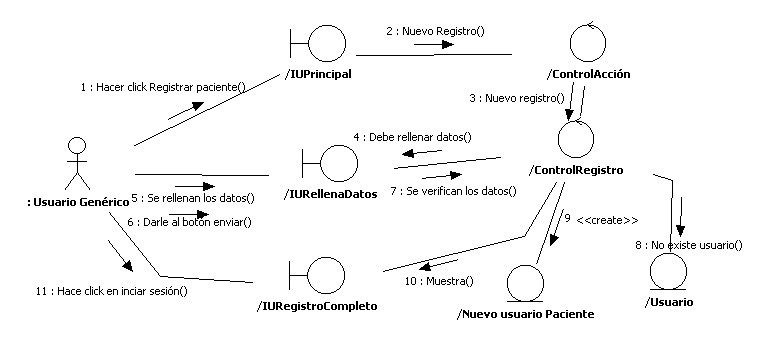
\includegraphics[width=16cm]{img/jpg/colaboraciones/17_Registrarse_paciente.jpg}
		  \caption{Registrarse como paciente}
		  \label{fig:col_reg_paciente}
		\end{figure}
	
		\begin{figure}[H]
		  \centering
		    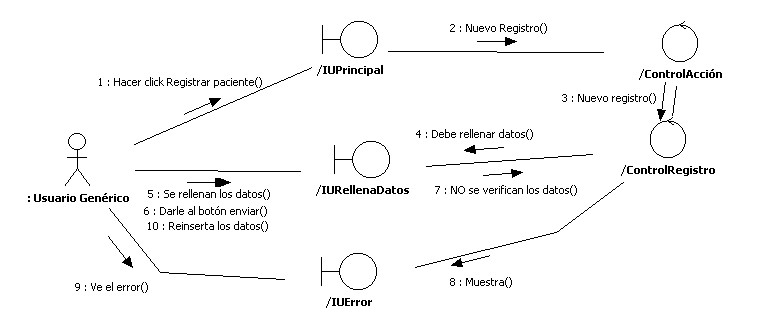
\includegraphics[width=16cm]{img/jpg/colaboraciones/18_RegistrarsePacienteError.jpg}
		  \caption{Error.- Registrarse como paciente}
		  \label{fig:col_reg_paciente_err}
		\end{figure}
		
		Una vez hemos realizado el registro, pasamos a las interfaces de rellenar datos. En función del rol de cada usuario, deberá rellenar unos datos u otros. Al finalizar, puede estar todo correcto (Figura \ref{fig:col_rellenarinfo}), o por el contrario puede aparecer algún error si no se verifica algún tipo de dato (Figura \ref{fig:col_rellenarinfo_err}).
		
		\begin{figure}[H]
		  \centering
		    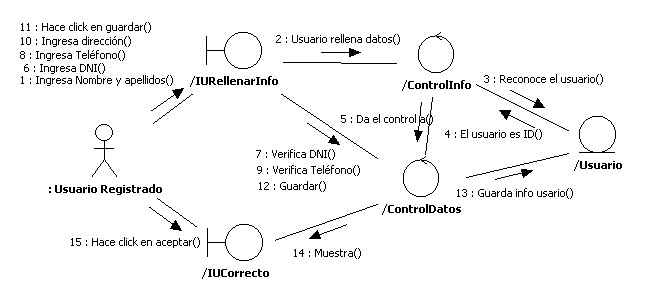
\includegraphics[width=16cm]{img/jpg/colaboraciones/19_RellenarInfo.jpg}
		  \caption{Rellenar información}
		  \label{fig:col_rellenarinfo}
		\end{figure}
		
		\begin{figure}[H]
		  \centering
		    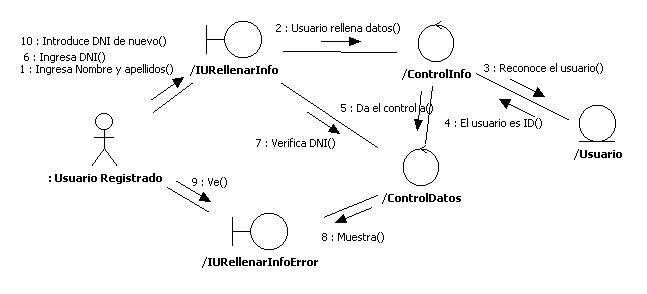
\includegraphics[width=16cm]{img/jpg/colaboraciones/20_RellenarInfoError.jpg}
		  \caption{Error.- Rellenar información}
		  \label{fig:col_rellenarinfo_err}
		\end{figure}
		
		Además, en el caso de ser médico, se debe rellenar información relativa a la consulta (Figura \ref{fig:col_rellenarinfo_consulta}), cómo puede ser la dirección, el teléfono de contacto, el precio, la especialidad, etcétera.
		
		\begin{figure}[H]
		  \centering
		    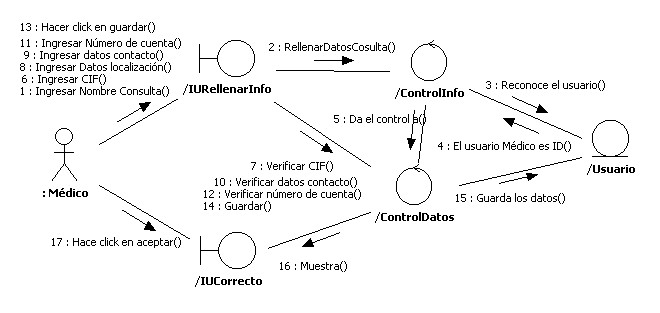
\includegraphics[width=16cm]{img/jpg/colaboraciones/21_RellenarInfoConsulta.jpg}
		  \caption{Rellenar información de la consulta}
		  \label{fig:col_rellenarinfo_consulta}
		\end{figure}
		
		\newpage
		Una vez que un usuario está registrado, podrá acceder a la aplicación (Figura \ref{fig:col_acc_y_aut}). Se identifica mediante el email y una contraseña. El sistema verifica que el usuario exista y que la contraseña sea correcta y se crea una nueva sesión y se accederá al \textit{dashboard}. Pueden aparecer errores, por ejemplo, si no existe el usuario, o si la contraseña introducida no es correcta. En dicho caso, se informará del error al usuario (Figura \ref{fig:col_acc_y_aut}).
		
		\begin{figure}[H]
		  \centering
		    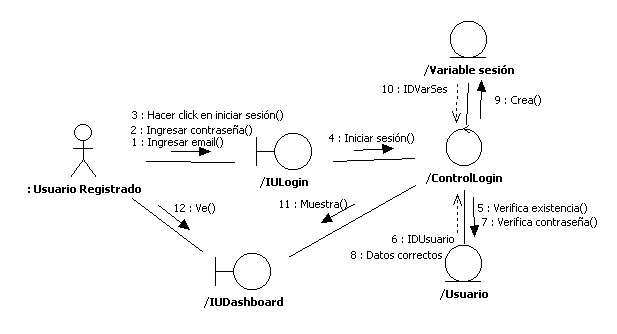
\includegraphics[width=16cm]{img/jpg/colaboraciones/23_Accesoyautentificacion.jpg}
		  \caption{Acceso y autentificación}
		  \label{fig:col_acc_y_aut}
		\end{figure}
		
		\begin{figure}[H]
		  \centering
		    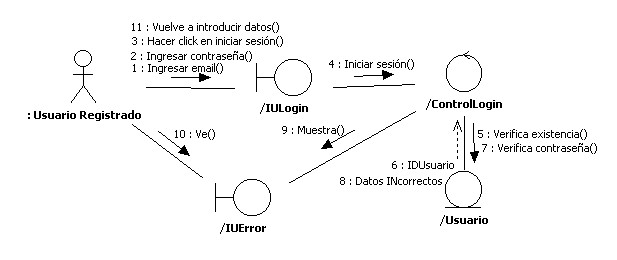
\includegraphics[width=16cm]{img/jpg/colaboraciones/24_AccesoyautentificacionError.jpg}
		  \caption{Error.- Acceso y autentificación}
		  \label{fig:col_acc_y_aut_err}
		\end{figure}
		
		Entre otras cosas, un usuario genérico podrá buscar cualquier médico antes de registrarte en el sistema para saber si le interesa (Figura \ref{fig:col_buscarmedico}). Si no encuentra ninguno, se notificará de que el médico no forma parte de la comunidad. Si lo encuentra, ofrece la posibilidad de ver su información.
		
		\begin{figure}[H]
		  \centering
		    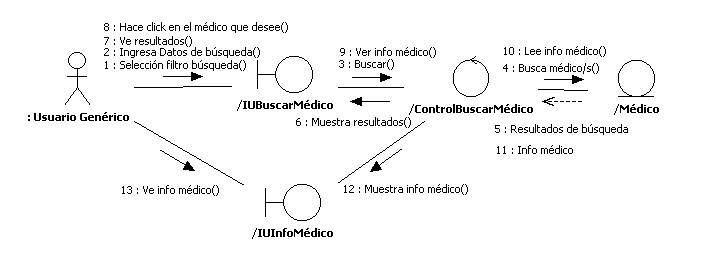
\includegraphics[width=16cm]{img/jpg/colaboraciones/22_BuscarMedico.jpg}
		  \caption{Buscar Médico}
		  \label{fig:col_buscarmedico}
		\end{figure}
		
		El resto de casos de uso relacionados con las \textit{Actividades Generales} son muy simples y son necesarios diagramas de colaboración.
		
	% subsection colaboraciones_de_las_actividades_generales (end)
	
	\newpage
	\subsection{Colaboraciones de los Médicos} % (fold)
	\label{sub:colaboraciones_de_los_medicos}
	
		En esta sección aparecen los principales diagramas de colaboraciones referentes a las actividades de los médicos.
		
		En primer lugar vemos que un médico debe realizar la configuración de sus datos. Si es la primera vez que accede al sistema, será lo primero con lo que se encuentre. En otro caso, siempre podrá acceder a los datos de su configuración en cualquier momento que lo desee. Si se produce algún cambio en la configuración, se almacenará dicho cambio en el \textit{historial del médico}. 
		
		Si la secuencia de acciones ha ocurrido correctamente, se mostrará un mensaje informando de que se ha actualizado la configuración con éxito (Figura \ref{fig:col_config_dat_medico}). Por el contrario, si se introduce algún tipo de datos incorrecto o con un formato no adecuado se producirá un error (Figura \ref{fig:col_config_dat_medico_err}). También pueden existir errores en el caso de que todos los datos introducidos sean en principio correctos, pero no se puedan almacenar o guardar en el usuario correspondiente (Figura \ref{fig:col_config_dat_medico_err2}).
		%\begin{landscape}
		\bigskip
		
		\begin{figure}[H]
		  \centering
		    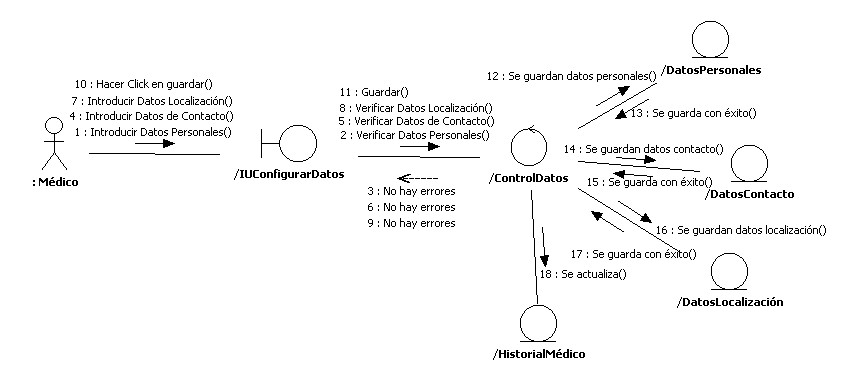
\includegraphics[width=16cm]{img/jpg/colaboraciones/1_ConfiguracionDatosMedico.jpg}
		  \caption{Configuración de los datos del médico}
		  \label{fig:col_config_dat_medico}
		\end{figure}
		
		\bigskip
		\bigskip
		\bigskip
		\begin{figure}[H]
		  \centering
		    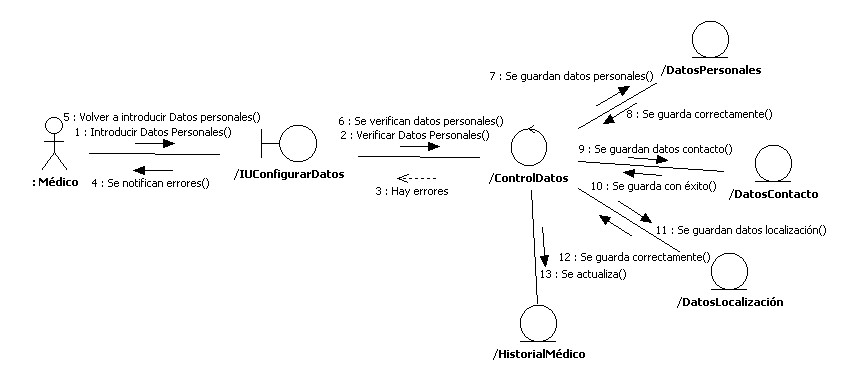
\includegraphics[width=16cm]{img/jpg/colaboraciones/2_ConfiguracionDatosMedicoError1.jpg}
		  \caption{Error.- Configuración de los datos del médico}
		  \label{fig:col_config_dat_medico_err}
		\end{figure}
		
		\bigskip
		\bigskip
		\bigskip
		\begin{figure}[H]
		  \centering
		    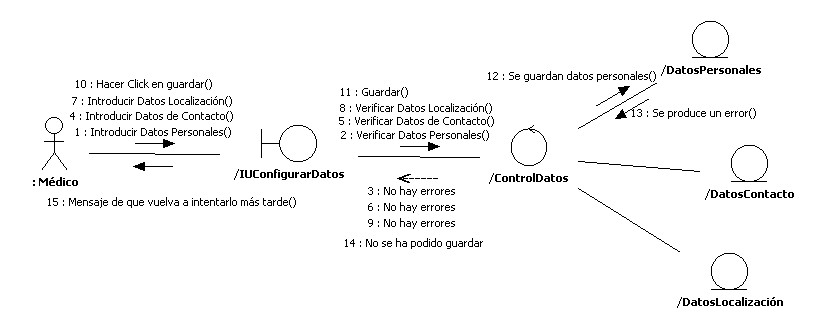
\includegraphics[width=16cm]{img/jpg/colaboraciones/3_ConfiguracionDatosMedicoError2.jpg}
		  \caption{Error.- Configuración de los datos del médico}
		  \label{fig:col_config_dat_medico_err2}
		\end{figure}
		
		\newpage
		
		Además de poder modificar su información personal, un médico puede realizar cambios en los datos de su cuenta, como son, por ejemplo, el email, nombre de usuario o la contraseña (Figura \ref{fig:col_config_cuenta_medico}). Si no existe ningún error (Figura \ref{fig:col_config_cuenta_medico_err}), se guardarán los cambios, se actualizará el \textit{historial del médico} y se informará de que todo ha ido correctamente. En caso contrario, se notificará al usuario el motivo del error y que sus cambios no han sido realizados.
		\begin{figure}[H]
		  \centering
		    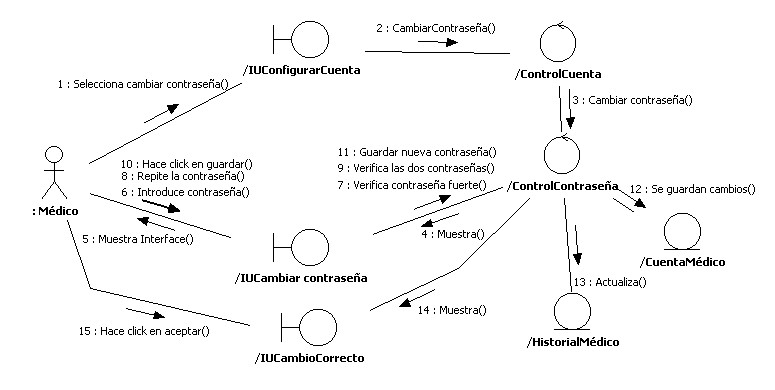
\includegraphics[width=16cm]{img/jpg/colaboraciones/4_ConfiguracionCuentaMedico.jpg}
		  \caption{Configuración de la cuenta del médico}
		  \label{fig:col_config_cuenta_medico}
		\end{figure}
		
		\begin{figure}[H]
		  \centering
		    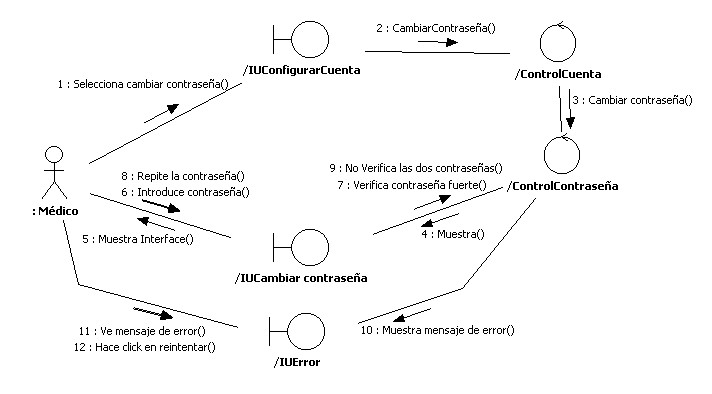
\includegraphics[height=7cm, width=16cm]{img/jpg/colaboraciones/5_ConfiguracionCuentaMedicoError.jpg}
		  \caption{Error.- Configuración de la cuenta del médico}
		  \label{fig:col_config_cuenta_medico_err}
		\end{figure}
		
		Uno de los aspectos fundamentales que debe configurar un médico es su horario, introduciendo principalmente \textit{cuales son sus días laborales, el rango de horas de su jornada laboral o su precio medio}. Podrá modificar esta información en cualquier momento que lo desee. Si la secuencia de acciones es validada y, por tanto, correcta, se guardarán los cambios en su horario, se actualizará el \textit{historial del médico} y se notificará (Figura \ref{fig:col_config_horario_medico}). Por el contrario, si algún dato no se verifica o si no se puede guardar la información en ese momento por cualquier motivo, se mostrará un mensaje notificando dicho fallo (Figura \ref{fig:col_config_horario_medico_err}).
		
		\begin{figure}[H]
		  \centering
		    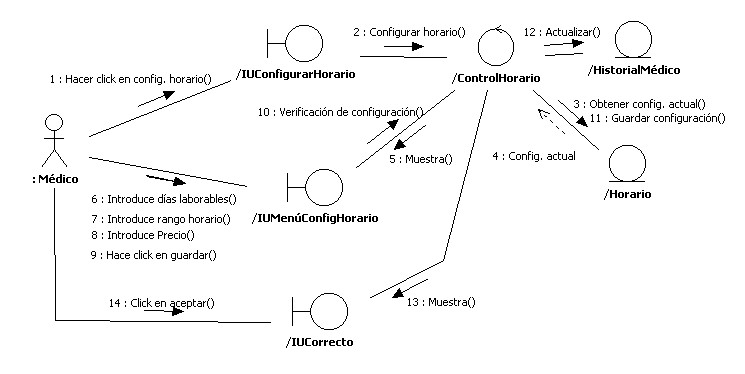
\includegraphics[width=16cm, height=7cm]{img/jpg/colaboraciones/6_ConfiguracionHorarioMedico.jpg}
		  \caption{Configuración del horario del médico}
		  \label{fig:col_config_horario_medico}
		\end{figure}
		
		\begin{figure}[H]
		  \centering
		    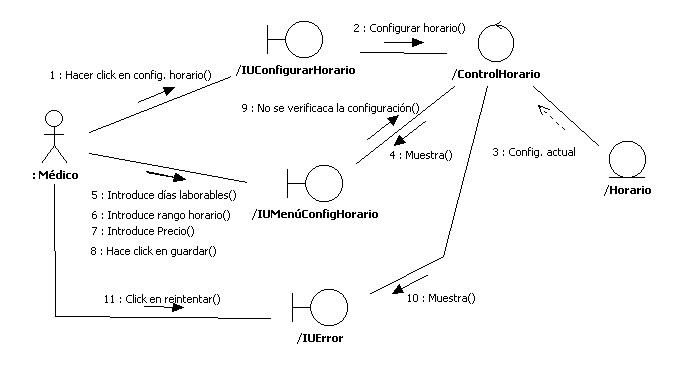
\includegraphics[width=16cm, height=7cm]{img/jpg/colaboraciones/7_ConfiguracionHorarioMedicoError.jpg}
		  \caption{Error.- Configuración del horario del médico}
		  \label{fig:col_config_horario_medico_err}
		\end{figure}
		
		El médico podrá ver un horario en vista semanal con las citas que tiene asignadas (Figura \ref{fig:col_vistasemanal_medico}). Además, desde dicha vista podrá ver la ficha médica de sus pacientes (Figura \ref{fig:col_verficha_medico}) y anular una cita puntual (Figura \ref{fig:col_anular_medico}).
		
		\begin{figure}[H]
		  \centering
		    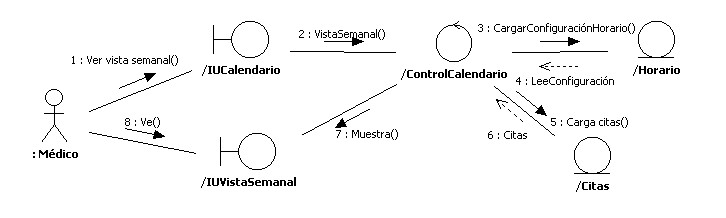
\includegraphics[width=16cm]{img/jpg/colaboraciones/8_VistaSemanalMedico.jpg}
		  \caption{Vista semanal del médico}
		  \label{fig:col_vistasemanal_medico}
		\end{figure}
		
		Anular una cita puntual (Figura \ref{fig:col_anular_medico}) requiere confirmación. Además, puede escribir el mensaje que le llegará al afectado. Quedará registrado en el \textit{historial del médico y en el del paciente}.
		\begin{figure}[H]
		  \centering
		    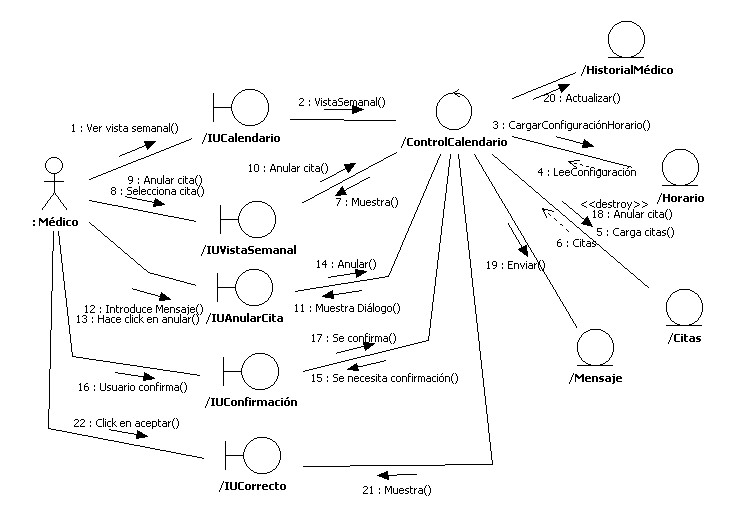
\includegraphics[width=16cm, height=10.5cm]{img/jpg/colaboraciones/9_AnularCitaMedico.jpg}
		  \caption{El médico anula una cita}
		  \label{fig:col_anular_medico}
		\end{figure}
		
		A la hora de anular una cita (Figura \ref{fig:col_anular_medico}), un médico siempre podrá retractarse y cancelar la acción (Figura \ref{fig:col_cancelaranular_medico}). Por eso, entre otras cosas, debe existir confirmación.
		
		\begin{figure}[H]
		  \centering
		    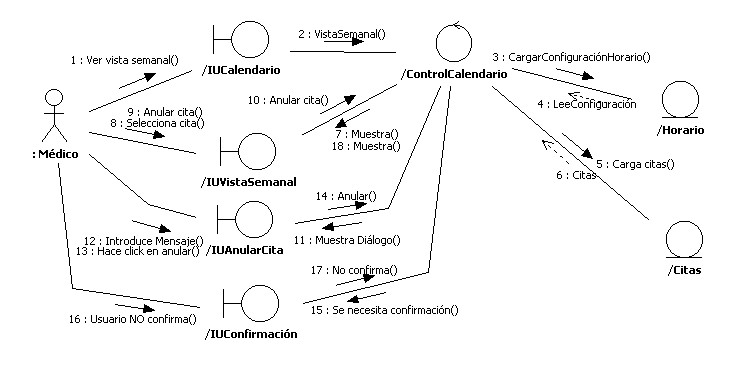
\includegraphics[width=16cm]{img/jpg/colaboraciones/10_AnularCitaMedicoCancelar.jpg}
		  \caption{El médico cancela anular una cita}
		  \label{fig:col_cancelaranular_medico}
		\end{figure}
		
		Un médico, además, podrá ver la ficha médica de un paciente (Figura \ref{fig:col_verficha_medico}). Ésta acción podrá realizarla tanto después de realizar una búsqueda de uno de sus pacientes como desde el calendario. Puede ir todo correcto, o por el contrario aparecer algún error inusual (Figura \ref{fig:col_verficha_medico_err}).
		
		\begin{figure}[H]
		  \centering
		    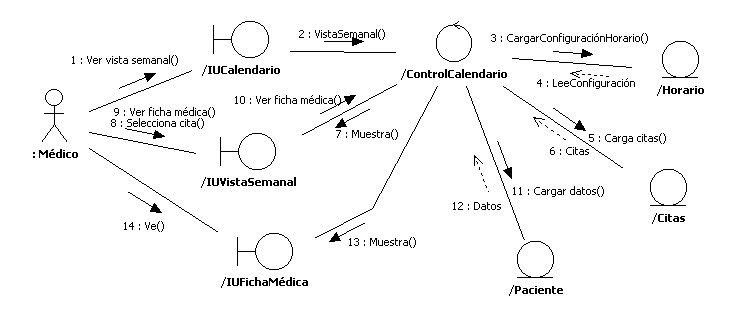
\includegraphics[width=16cm]{img/jpg/colaboraciones/11_VerFichaMedica.jpg}
		  \caption{El médico ve una ficha médica}
		  \label{fig:col_verficha_medico}
		\end{figure}
		
		\begin{figure}[H]
		  \centering
		    \includegraphics[width=16cm]{img/jpg/colaboraciones/12_VerFichaMedicaError.jpg}
		  \caption{Error.- Médico viendo una ficha médica}
		  \label{fig:col_verficha_medico_err}
		\end{figure}
		
		Otra de las acciones que puede realizar un usuario con rol de médico es ver la lista de todos sus pacientes (Figura \ref{fig:col_ver_pacientes_medico}). Puede que en dicho momento ocurra un error de acceso, el cuál será notificado inmediatamente (Figura \ref{fig:col_ver_pacientes_medico_err}).
		
		\begin{figure}[H]
		  \centering
		    \includegraphics[width=16cm]{img/jpg/colaboraciones/13_VerTodosPacientes.jpg}
		  \caption{El médico ve la lista de sus pacientes}
		  \label{fig:col_ver_pacientes_medico}
		\end{figure}
		
		\begin{figure}[H]
		  \centering
		    \includegraphics[width=16cm]{img/jpg/colaboraciones/14_VerTodosPacientesError.jpg}
		  \caption{Error.- El médico ve la lista de sus pacientes}
		  \label{fig:col_ver_pacientes_medico_err}
		\end{figure}
		
		La última de las principales acciones será la de buscar un paciente concreto (Figura \ref{fig:col_buscarpaciente_medico}). Ésta acción se puede llevar a cabo mediante distintos tipos de búsqueda. Si no encuentra ningún paciente, o si se produce algún error, se notificará mediante la interfaz (Figura \ref{fig:col_buscarpaciente_medico_err}).
		
		\begin{figure}[H]
		  \centering
		    \includegraphics[width=16cm]{img/jpg/colaboraciones/15_BuscarPaciente.jpg}
		  \caption{Buscar Paciente}
		  \label{fig:col_buscarpaciente_medico}
		\end{figure}
		
		\begin{figure}[H]
		  \centering
		    \includegraphics[width=16cm]{img/jpg/colaboraciones/16_BuscarPacienteError.jpg}
		  \caption{Error.- Buscar paciente}
		  \label{fig:col_buscarpaciente_medico_err}
		\end{figure}
		
	% subsection colaboraciones_de_los_médicos (end)
	
	\newpage
	\subsection{Colaboraciones de los Pacientes} % (fold)
	\label{sub:colaboraciones_de_los_pacientes}
				
		Los diagramas de colaboraciones relacionados con la configuración de la información personal y de los datos de la cuenta del usuario con rol paciente, son prácticamente los mismos que los ya vistos para los usuarios con rol de médico. Las pequeñas diferencias son que las entidades serán los pacientes (en lugar de médicos), y que se modificará el \textit{historial del paciente (en lugar de el historial del médico)}.
		
		Por su parte, un paciente también podrá ver una vista semanal de su calendario, con las citas que tiene previstas (Figura \ref{fig:col_vistasemanal_paciente}). Desde ella podrá ver la información del médico (Figura \ref{fig:col_verinfo_medico_paciente}) y anular una cita (Figura \ref{fig:col_anulacita_paciente}).
		
		\bigskip
		\bigskip
		\begin{figure}[H]
		  \centering
		    \includegraphics[width=16cm]{img/jpg/colaboraciones/25_VistaSemanalPaciente.jpg}
		  \caption{Vista semanal del paciente}
		  \label{fig:col_vistasemanal_paciente}
		\end{figure}
		
		\bigskip
		\bigskip
		
		Cuando un paciente anula una cita, debe tener en cuenta que sea antes de la fecha y hora concebida para poder hacerlo sin recibir ningún recargo. 
		
		Esta acción siempre requiere confirmación por parte del usuario. Si llega a anularse, se guardará el registro de lo ocurrido en el \textit{historial del médico y en el historial del paciente}. Una vez anulado, se notificará mediante la interfaz (Figura \ref{fig:col_anulacita_paciente}). Además, tanto al médico como al paciente les llegará un email informando de que la cita ha sido cancelada (en el caso de que así lo tengan configurado).
		
		Por otro lado, una vez hemos entrado en el camino de anular una cita, siempre tendremos la posibilidad de cancelar la acción, o bien de no confirmarla (Figura \ref{fig:col_anularcita_paciente_cancelar}).
		
		Podemos ver que es un diagrama de colaboración bastante similar al de anular cita de un médico (Figura \ref{fig:col_anular_medico}).
		
		\begin{figure}[H]
		  \centering
		    \includegraphics[width=16cm]{img/jpg/colaboraciones/26_AnularCitaPaciente.jpg}
		  \caption{El paciente anula una cita}
		  \label{fig:col_anulacita_paciente}
		\end{figure}
		
		\begin{figure}[H]
		  \centering
		    \includegraphics[width=16cm]{img/jpg/colaboraciones/27_AnularCitaPacienteCancelar.jpg}
		  \caption{El paciente cancela anular una cita}
		  \label{fig:col_anularcita_paciente_cancelar}
		\end{figure}
		
		Tanto desde la vista semanal, cómo si se ha realizado una búsqueda, un paciente podrá ver la información de un médico (Figura \ref{fig:col_verinfo_medico_paciente}). Si no se produce ningún error, se mostrará la información. En caso contrario, se notificará mediante la interfaz. Además, esta acción también puede ser usada por un usuario genérico tras buscar un médico desde el \textit{Home} de la página web.
		
		\begin{figure}[H]
		  \centering
		    \includegraphics[width=16cm]{img/jpg/colaboraciones/28_VerInfoMedico.jpg}
		  \caption{Ver información de un médico}
		  \label{fig:col_verinfo_medico_paciente}
		\end{figure}
		
		Un paciente, además, podrá realizar búsquedas de médicos en función de diversos filtros (Figura \ref{fig:col_buscarmedico_paciente}). En el caso de no encontrar resultados o de que exista algún error, se informará al usuario.
		
		\begin{figure}[H]
		  \centering
		    \includegraphics[width=16cm]{img/jpg/colaboraciones/29_PacienteBuscarMedico.jpg}
		  \caption{El paciente busca un médico}
		  \label{fig:col_buscarmedico_paciente}
		\end{figure}
		
		\bigskip
		\bigskip
		Una vez hemos realizada la búsqueda de un médico, podremos ver su horario, y además, asignarnos una cita. La vista del horario nos proporcionará gráficamente las horas libres de las que dispone el médico (Figura \ref{fig:col_verhorario_paciente}). En caso de querer asignarnos una cita (Figura \ref{fig:col_asigcita_paciente}), seleccionaremos la que más nos convenga. Si todo ocurrió correctamente, se guardará un registro en el \textit{historial del médico y en el del paciente} y se enviarán las correspondiente notificaciones vía email (si así lo tienen configurado).
		
		\begin{figure}[H]
		  \centering
		    \includegraphics[width=16cm]{img/jpg/colaboraciones/30_VerhoarioMedico.jpg}
		  \caption{Ver el horario de un médico}
		  \label{fig:col_verhorario_paciente}
		\end{figure}
		
		\begin{figure}[H]
		  \centering
		    \includegraphics[width=16cm]{img/jpg/colaboraciones/31_AsignarseCita.jpg}
		  \caption{Asignarse una cita}
		  \label{fig:col_asigcita_paciente}
		\end{figure}
		
		
	% subsection colaboraciones_de_los_pacientes (end)

	\newpage
	\subsection{Colaboraciones de las Fichas Médicas} % (fold)
	\label{sub:colaboraciones_de_las_fichas_medicas}
	
		Hay una serie de actividades relacionadas con las fichas médicas que pueden realizar tanto médicos como pacientes. Todas ellas son bastante similares.
		
		En primer lugar tenemos las colaboraciones relacionadas con los antecedentes (pueden ser fisiológicos, familiares y personales). Vamos a representar sólo los fisiológicos, siendo el resto muy similares.
		
		Podremos ver una lista con los antecedentes (Figura \ref{fig:col_ant_fis_fm}), así como también añadir nuevos (\ref{fig:col_ant_fis_fm_anadir}) o modificar los existentes (Figura \ref{fig:col_ant_fis_fm_modificar}).
		
		\bigskip
		\bigskip
		\begin{figure}[H]
		  \centering
		    \includegraphics[width=16cm]{img/jpg/colaboraciones/32_VerAntecedentesFisiologicos.jpg}
		  \caption{Ver los antecedentes fisiológicos}
		  \label{fig:col_ant_fis_fm}
		\end{figure}
		
		\bigskip
		En el caso de añadir antecedentes (Figura \ref{fig:col_ant_fis_fm_anadir}), debemos tener en cuenta de que tipo son (en este diagrama son fisiológicos), y asegurarnos del paciente al que pertenecen. Una vez hecho esto, se creará el antecedente, se nos mostrará una nueva interfaz en la que deberemos rellenar los datos correspondientes, los cuales deben ser verificados por la unidad de control antes de guardarse y actualizarse. Si el antecedente se crea y se guarda correctamente, se informará al usuario y se mostrará la lista de los antecedentes. Además, se modificará el \textit{historial de la ficha médica}.
		
		Si existiese algún error (Figura \ref{fig:col_ant_fis_fm_anadir_err}) a la hora de crear el antecedente o de introducir la información, se notificaría al usuario.
		
		A la hora de realizar modificaciones en algún antecedente (Figura \ref{fig:col_ant_fis_fm_modificar}), el proceso es muy similar al de \textit{añadirlos}. En este caso, deberemos seleccionar un antecedente de los que ya existen, y a partir de ahí deberemos modificar los datos en la interfaz correspondiente. Si los datos introducidos son correctos y se actualiza correctamente, se mostrará un mensaje informando de que el proceso ha salido bien y se volverá a mostrar la lista de antecedentes. Si aparece algún error, se notificará al usuario (Figura \ref{fig:col_ant_fis_fm_modificar_err})
		
		\bigskip
		\bigskip
		\begin{figure}[H]
		  \centering
		    \includegraphics[width=16cm]{img/jpg/colaboraciones/33_AnadirAntecedente.jpg}
		  \caption{Añadir antecedentes fisiológicos}
		  \label{fig:col_ant_fis_fm_anadir}
		\end{figure}
		
		\bigskip
		\bigskip
		\begin{figure}[H]
		  \centering
		    \includegraphics[width=16cm]{img/jpg/colaboraciones/34_AnadirAntecedenteError.jpg}
		  \caption{Error.- Añadir antecedentes fisiológicos}
		  \label{fig:col_ant_fis_fm_anadir_err}
		\end{figure}
		
		\begin{figure}[H]
		  \centering
		    \includegraphics[width=16cm]{img/jpg/colaboraciones/35_ModificarAntecedente.jpg}
		  \caption{Modificar antecedentes fisiológicos}
		  \label{fig:col_ant_fis_fm_modificar}
		\end{figure}
		
		\begin{figure}[H]
		  \centering
		    \includegraphics[width=16cm]{img/jpg/colaboraciones/36_ModificarAntecedenteError.jpg}
		  \caption{Error.- Modificar antecedentes fisiológicos}
		  \label{fig:col_ant_fis_fm_modificar_err}
		\end{figure}
		
		
		\newpage
		Con los diagnósticos, así como con el resto de posibles tipos de pruebas, los diagramas de colaboraciones son muy similares, cambiando principalmente la entidad (antecedente, diagnóstico, etcétera) en función de su tipo. Encontraremos la posibilidad de ver, añadir y modificar diagnósticos, tratamientos, observaciones, pruebas varias, etcétera.
		
		A continuación se muestran las colaboraciones relacionadas con los diagnósticos.
		\begin{figure}[H]
		  \centering
		    \includegraphics[width=16cm]{img/jpg/colaboraciones/37_VerDiagnosticos.jpg}
		  \caption{Ver diagnósticos}
		  \label{fig:col_diag_fm}
		\end{figure}
		
		\begin{figure}[H]
		  \centering
		    \includegraphics[width=16cm]{img/jpg/colaboraciones/38_AnadirDiagnostico.jpg}
		  \caption{Añadir diagnósticos}
		  \label{fig:col_diag_fm_anadir}
		\end{figure}
		
		\begin{figure}[H]
		  \centering
		    \includegraphics[width=16cm]{img/jpg/colaboraciones/39_AnadirDiagnosticoError.jpg}
		  \caption{Error.- Añadir diagnósticos}
		  \label{fig:col_diag_fm_anadir_err}
		\end{figure}
		
		\begin{figure}[H]
		  \centering
		    \includegraphics[width=16cm]{img/jpg/colaboraciones/40_ModificarDiagnostico.jpg}
		  \caption{Modificar diagnósticos}
		  \label{fig:col_diag_fm_modificar}
		\end{figure}
		
		\begin{figure}[H]
		  \centering
		    \includegraphics[width=16cm]{img/jpg/colaboraciones/41_ModificarDiagnosticoError.jpg}
		  \caption{Error.- Modificar diagnósticos}
		  \label{fig:col_diag_fm_modificar_error}
		\end{figure}
		
	% subsection colaboraciones_de_las_fichas_médicas (end)

	\newpage
	\subsection{Colaboraciones del Administrador} % (fold)
	\label{sub:colaboraciones_del_administrador}
	
		El principal diagrama de colaboración que debemos ver en esta sección es el de verificar médico. Una vez verificado, se hará visible para el resto de usuarios y se le notificará de que su cuenta está activa.
		
		\begin{figure}[H]
		  \centering
		    \includegraphics[width=16cm]{img/jpg/colaboraciones/42_VerificarMedico.jpg}
		  \caption{Verificar médico}
		  \label{fig:col_verificar_admin}
		\end{figure}
	
	% subsection colaboraciones_del_administrador (end)
	
% section diagrama_de_lolaboraciones (end)

 % Diagrama de colaboraciones
		\section{Diagrama de clases del análisis} % (fold)
\label{sec:diagrama_de_clases_analisis}

\subsection{Actividades generales} % (fold)
\label{sub:actividades_generales}
	
	En primer lugar podemos ver el diagrama referente a los nuevos registros tanto de pacientes como de médicos (Figura \ref{fig:col_clase7}).
	\begin{figure}[H]
	  \centering
	    \includegraphics[width=15cm, height= 7cm]{img/jpg/clases/7_Registrarse.jpg}
	  \caption{Registrarse}
	  \label{fig:col_clase7}
	\end{figure}

	Una vez realizado el registro, se deben rellenar una serie de datos (Figura \ref{fig:col_clase8})
	\begin{figure}[H]
	  \centering
	    \includegraphics[width=15cm, height=7cm]{img/jpg/clases/7_RellenarInfo.jpg}
	  \caption{Rellenar información}
	  \label{fig:col_clase8}
	\end{figure}
	
	A continuación un diagrama muy general (Figura \ref{fig:col_clase9}), en el que se muestran el resto de actividades generales que pueden realizar los usuarios genéricos. Éstas son buscar médico, términos legales, condiciones de uso, contactar con el administrador, preguntas frecuentes y cambiar idioma.
	\begin{figure}[H]
	  \centering
	    \includegraphics[width=16cm]{img/jpg/clases/8_Varios.jpg}
	  \caption{Otras actividades}
	  \label{fig:col_clase9}
	\end{figure}
	
	\newpage
	Por último, el diagrama relacionado con el acceso y autentificación (Figura \ref{fig:col_clase10}) para iniciar una nueva sesión. Tras el acceso, se va al dashboard del médico o del paciente
	\begin{figure}[H]
	  \centering
	    \includegraphics[width=12cm]{img/jpg/clases/9_AccesoYAutentificacion.jpg}
	  \caption{Acceso y autentificación}
	  \label{fig:col_clase10}
	\end{figure}

% subsection actividades_generales (end)

\newpage
\subsection{Médicos} % (fold)
\label{ssub:medicos}

	En primer lugar podemos ver todo lo relacionado con la configuración del médico (Figura \ref{fig:col_clase1}), que a su vez se verá con más detalle en los siguientes diagramas. Las posibles cosas que se pueden configurar son la información, la cuenta, el horario, las notificaciones y los motivos.
	\begin{figure}[H]
	  \centering
	    \includegraphics[width=16cm]{img/jpg/clases/1_MedicoConfiguracion.jpg}
	  \caption{Configuración del médico}
	  \label{fig:col_clase1}
	\end{figure}
	
	\newpage
	A la hora de configurar los datos (Figura \ref{fig:col_clase2}), en principio, serán los datos personales, los de localización y los de contacto.
	\begin{figure}[H]
	  \centering
	    \includegraphics[width=12cm, height=5cm]{img/jpg/clases/2_MedicosConfiguracionDatos.jpg}
	  \caption{Configuración de los datos del médico}
	  \label{fig:col_clase2}
	\end{figure}

	En la configuración de la cuenta (Figura \ref{fig:col_clase3}), observamos que principalmente se puede cambiar el email, la contraseña y el idioma. Además, podrá darse de baja del servicio. Si se modifica la configuración, se guardará un registro en el \textit{historial del médico}.
	\begin{figure}[H]
	  \centering
	    \includegraphics[width=16cm, height=10cm]{img/jpg/clases/3_MedicoConfiguracionCuenta.jpg}
	  \caption{Configuración de la cuenta del médico}
	  \label{fig:col_clase3}
	\end{figure}
	
	Un médico también podrá configurar su horario (Figura \ref{fig:col_clase4}).
	\begin{figure}[H]
	  \centering
	    \includegraphics[width=12cm, height=6cm]{img/jpg/clases/4_MedicoConfiguracionHorario.jpg}
	  \caption{Configuración del horario del médico}
	  \label{fig:col_clase4}
	\end{figure}

	Por otro lado, un médico tiene que poder ser capaz de ver sus calendarios (Figura \ref{fig:col_clase5}), en distintos tipos de vista. En ellos aparecerán las citas que tienen concertadas, y debe ser capaz de anular una concreta o de ver la información de la ficha médica de sus pacientes. Además, al anular una cita se le enviará un mensaje al paciente.
	\begin{figure}[H]
	  \centering
	    \includegraphics[width=16cm, height=9cm]{img/jpg/clases/5_CalendarioMedico.jpg}
	  \caption{Calendario del médico}
	  \label{fig:col_clase5}
	\end{figure}
	
	
	El último de los principales diagramas de clases relacionados con los médicos es el de sus pacientes (Figura \ref{fig:col_clase6}). Podrá buscarlos de distintas maneras y ver su información.
	\begin{figure}[H]
	  \centering
	    \includegraphics[width=16cm]{img/jpg/clases/6_MedicosPacientes.jpg}
	  \caption{Pacientes del médico}
	  \label{fig:col_clase6}
	\end{figure}

% subsubsection médicos (end)

\newpage
\subsection{Pacientes} % (fold)
\label{sub:pacientes}

Respecto a los pacientes, los diagramas de clases relacionados con la configuración de los datos y de la información son prácticamente iguales que los diagramas de los médicos.

Por otro lado, un paciente tiene que poder ser capaz de ver sus calendarios (Figura \ref{fig:col_clase11}), en distintos tipos de vista. En ellos aparecerán las citas que tienen concertadas, y debe ser capaz de anular una concreta o de ver la información de sus médicos. Además, al anular una cita se le enviará un mensaje al médico.
\begin{figure}[H]
  \centering
    \includegraphics[width=16cm]{img/jpg/clases/10_PacientesCalendario.jpg}
  \caption{Calendario del paciente}
  \label{fig:col_clase11}
\end{figure}

\newpage
El último de los principales diagramas de clases relacionados con los pacientes es el de sus médicos (Figura \ref{fig:col_clase12}). Podrá buscarlos de distintas maneras y ver su información y sus horarios.
\begin{figure}[H]
  \centering
    \includegraphics[width=16cm]{img/jpg/clases/11_PacientesMedicos.jpg}
  \caption{Buscar los médicos de un paciente}
  \label{fig:col_clase12}
\end{figure}
% subsection pacientes (end)

\newpage
\subsection{Ficha médica} % (fold)
\label{sub:ficha_medica}

	Una ficha médica abarca muchos tipos de datos y de pruebas. Entre otros, los antecedentes (de diversos tipos), diagnósticos, tratamientos, pruebas etcétera. En el primer diagrama (Figura \ref{fig:col_clase13}) vemos en detalle lo relacionado con los antecedentes.
	\begin{figure}[H]
	  \centering
	    \includegraphics[width=16cm]{img/jpg/clases/12_Antecedentes.jpg}
	  \caption{Antecedentes}
	  \label{fig:col_clase13}
	\end{figure}

	\newpage
	En este diagrama (Figura \ref{fig:col_clase14}) encontramos lo relacionado con los informes, los tratamientos, los diagnósticos y las distintas posibles exploraciones clínicas.
	\begin{figure}[H]
	  \centering
	    \includegraphics[width=16cm]{img/jpg/clases/13_Resto.jpg}
	  \caption{Resto de casos.}
	  \label{fig:col_clase14}
	\end{figure}
% subsection ficha_médica (end)
	
\newpage
\subsection{Administrador} % (fold)
\label{sub:administrador}
	Por último tenemos el diagrama de clases relacionado con el administrador del sistema. Éste podrá habilitar médicos, suspenderlos, verificar su licenciatura, responder a las preguntas de los usuarios, agregar nuevos administradores, modificar el contenido de los términos legares y de las condiciones de uso.
	\begin{figure}[H]
	  \centering
	    \includegraphics[width=16cm]{img/jpg/clases/14_Administrador.jpg}
	  \caption{Registrarse como paciente}
	  \label{fig:col_clase15}
	\end{figure}
	
% subsection administrador (end)

% section diagrama_de_clases (end)

 % Diagrama de clases del análisis
		\section{Diagrama de capas} % (fold)
\label{sec:diagrama_de_capas}

	Cualquier sistema grande se debe dividir en unidades más pequeñas, de modo que las personas puedan trabajar con una cantidad de información limitada, a la vez y de modo que los equipos de trabajo no interfieran con el trabajo de los otros. La gestión del modelo consiste en paquetes y relaciones de dependencia de los paquetes.
	
	Un paquete es, por tanto, una parte de un modelo. Además, cada parte de un modelo debe pertenecer a un paquete. El modelador puede asignar el contenido de un modelo a un conjunto de paquetes. Pero, para ser funcional, la asignación debe seguir un cierto principio racional, tal como funcionalidad común, implementación estrechamente relacionada, y un punto de vista común.
	
	UML no impone una regla para componer los paquetes, pero una buena descomposición en paquetes realzará enormemente la capacidad de mantenimiento del modelo. Pueden ser organizados por la vista, por la funcionalidad, o por cualquier otra base que el modelador elija.
	
	Los paquetes son unidades de organización jerárquica de uso general de los modelos UML, que contienen elementos del modelo al más alto nivel, y además, pueden contener otros paquetes. Si se eligen bien los paquetes, reflejan la arquitectura de alto nivel de un sistema: su descomposición en subsistemas y sus dependencias. Una dependencia entre paquetes resume las dependencias entre los contenidos del paquete.
	
	En nuestro caso, vamos a agrupar los paquetes en base a dos capas. \textbf{La capa específica y la capa genérica. (Figura \ref{fig:acapas})} 
	
	En la primera, se hace mención a los paquetes propios de la aplicación, como son todos aquellos relacionados con las \textit{Actividades de los médicos, de los pacientes, de las fichas médicas, del administrador y de los usuarios genéricos.} Además, todos estos paquetes se dividen en subpaquetes, para agrupar una serie de actividades más específicas de cada uno de ellos. 
	
	Por su parte, en la segunda, se agrupan una serie de paquetes que pueden ser reutilizados en otras aplicaciones. En este proyecto son los relacionados con el \textit{registro de usuarios, algunas librerías javascript, la función autocompletar, la posibilidad de realizar paginación y todo lo relacionado con el multilenguaje.}
	
	\begin{figure}[H]
	  \centering
	    \includegraphics[width=13cm]{img/jpg/acapas/capas.jpg}
	  \caption{Diagrama de Capas}
	  \label{fig:acapas}
	\end{figure}
	
	Una vez visto el diagrama general dividido en dos capas principales, con los subsistemas(paquetes) que contienen cada una de ellas, vamos a ver con más detalle los paquetes de la capa específica.
	
	En primer lugar, el paquete de \textit{Actividades de los médicos} (Figura \ref{fig:acapas_medicos}), que está compuesto por \textit{Gestión del horario, del calendario, de los pacientes, de las plantillas, de las estadísticas y la administración.}
	
	A continuación tenemos los paquetes en los que están divididas las \textit{Actividades de los pacientes} (Figura \ref{fig:acapas_pacientes}), que son \textit{la Gestión del calendario, de los médicos y de las fichas médicas.}
	
	Por último, vemos los paquetes que forman las \textit{Fichas médicas} (Figura \ref{fig:acapas_fichas}). Éstos son \textit{Gestión de antecedentes, de informes, de tratamientos, de exploraciones, de pruebas y de observaciones}.
	
	\begin{figure}[H]
	  \centering
	    \includegraphics[width=13cm]{img/jpg/acapas/Actividades_medicos.jpg}
	  \caption{Diagrama de Capas}
	  \label{fig:acapas_medicos}
	
	\begin{figure}[H]
	  \centering
	    \includegraphics[width=13cm]{img/jpg/acapas/Actividades_Pacientes.jpg}
	  \caption{Diagrama de Capas}
	  \label{fig:acapas_pacientes}
	\end{figure}
	
	\begin{figure}[H]
	  \centering
	    \includegraphics[width=13cm]{img/jpg/acapas/fichas_medicas.jpg}
	  \caption{Diagrama de Capas}
	  \label{fig:acapas_fichas}
	\end{figure}
	\end{figure}

% section diagrama_de_capas (end)
 % Diagrama de capas del análisis
	% chapter análisis (end)
	
	\chapter{Diseño} % (fold)
	\label{cha:diseno}
		% ----------------------------------
% Introducción al diseño
% ----------------------------------
 


		\textit{Si los productos se diseñan para que se ajusten mejor a las tendencias naturales del comportamiento humano, entonces las personas estarán más satisfechas, más complacidas y serán más productivas.}
		
	\section{Introducción} % (fold)
	\label{sec:introduccion}
	
		El diseño de una \textit{webapp} como la que nos atañe incluye actividades técnicas que abarcan diversos aspectos: establecer la vista y sensación de la \textit{webapp}, creando la distribución estética de la interfaz de usuario, definiendo la estructura arquitectónica general, desarrollando el contenido y la funcionalidad que residen en la arquitectura y planeando la navegación que ocurre dentro de la aplicación web.
		
		Es importante puesto que el diseño permite crear un modelo que se evalúe respecto de su calidad, para mejorarlo antes de la generación de contenido y código, de la realización de las pruebas y del involucramiento de un gran número de usuarios. El diseño es el lugar donde se establece la calidad de la \textit{webapp}.
		
		\fbox{\parbox{15cm}{El diseño es la actividad de la ingeniería que genera un producto de alta calidad.}}
		
		\bigskip
		\bigskip
		Podemos definir \textbf{la calidad} de una aplicación web en términos de:
		\begin{itemize}
			\item \textit{Usabilidad}.
				\begin{itemize}
					\item Comprensión global del sitio.
					\item Retroalimentación y ayuda en línea.
					\item Características y estética de la interfaz.
					\item Características especiales.
				\end{itemize}
			\item \textit{Funcionalidad.}
				\begin{itemize}
					\item Capacidad de búsqueda y de recuperación.
					\item Características de navegación y de conexión.
					\item Características relacionadas con el dominio de la aplicación.
				\end{itemize}
			\item \textit{Confiabilidad.}
				\begin{itemize}
					\item Procesamiento correcto de los vínculos.
					\item Recuperación de errores.
					\item Validación y recuperación de las entradas del usuario.
				\end{itemize}
			\item \textit{Eficiencia.}
				\begin{itemize}
					\item Desempeño del tiempo de respuesta.
					\item Velocidad de generación de la página.
					\item Velocidad de generación de los gráficos.
				\end{itemize}
			\item \textit{Facilidad para recibir mantenimiento.}
				\begin{itemize}
					\item Facilidad de corrección.
					\item Adaptabilidad.
					\item Extensibilidad.
				\end{itemize}
			\item \textit{Seguridad.}
				\begin{itemize}
					\item En bases de datos críticas.
					\item Capacidad para rechazar accesos no deseados.
					\item Capacidad para detener un ataque proveniente del exterior.
				\end{itemize}
			\item \textit{Disponibilidad.}
				\begin{itemize}
					\item Satisfacer las necesidades de los usuarios en todo momento.
				\end{itemize}
			\item \textit{Escalabilidad.}
			\item \textit{Tiempo para llegar al mercado.}
		\end{itemize}	
		
		Además, el diseño de la \textit{webapp} se propone un \textbf{conjunto de metas}, como son:
		\begin{itemize}
			\item \textit{Simplicidad.} El contenido debe ser informativo pero sucinto y debe utilizar un modo de entrega (texto, imágenes, etcétera) que resulte apropiado para la información que se envíe. La estética debe ser agradable pero no abrumadora. La arquitectura debe lograr los objetivos de la \textit{webapp} de la manera más sencilla posible. La navegación debe ser directa y sus mecanismos obvios para la intuición del usuario final. Las funciones deben ser fáciles de utilizar y más fáciles de entender.
			\item \textit{Consistencia.} Esta meta del diseño se aplica virtualmente a todo elemento del modelo del diseño. El contenido debe construirse de modo congruente. El diseño gráfico debe presentar una vista consistente en todas las partes de la \textit{webapp}. El diseño arquitectónico debe establecer plantillas que generen una estructura de hipermedios constante. El diseño de la interfaz debe definir modos consistentes de interacción, navegación y despliegue del contenido. Los mecanismos de navegación deben usarse de manera consistente en todos los elementos de la \textit{webapp}.
			\item \textit{Identidad.} El diseño de la estética, la interfaz y la navegación de una \textit{webapp} deben ser consistentes con el dominio de la aplicación para la que se va a elaborar. La identidad se logra por medio del diseño.
			\item \textit{Robustez.} Con base en la identidad que se establece, es frecuente que una \textit{webapp} transmita algo al usuario. Éste espera contenido y funciones robustas que sean relevantes para sus necesidades. Si no existen o son insuficientes, es probable que la aplicación fracase.
			\item \textit{Navegabilidad.} Ya se dijo que la navegación debe ser sencilla y consistente. También debe estar diseñada en forma tal que sea intuitiva y predecible. Es decir, el usuario debe comprender cómo moverse sin tener que buscar vínculos o instrucciones para la navegación.
			\item \textit{Atractivo visual.} De todas las categorías de software, las aplicaciones web son indiscutiblemente las más visuales, dinámicas y estéticas. El atractivo visual radica sin lugar a dudas en los ojos del espectador, pero muchas características del diseño (aspecto y sensación del contenido, distribución de la interfaz, coordinación del color, balance del texto, imágenes y otros medios) aumentan el atractivo visual.
		\end{itemize}
		
		\subsection{Pasos a seguir} % (fold)
		\label{sub:pasos_a_seguir}
		
			Para abordar todos los aspectos del diseño, incluiremos seis etapas principales (Figura \ref{fig:dis_piramide})que son orientadas por la información obtenida durante la modelación de los requerimientos de usuario. 
		   
		   \begin{figure}[H]
		     \centering
		       \includegraphics[width=6cm]{img/jpg/piramide.jpg}
		     \caption{Pirámide del diseño de la \textit{webapp}.}
		     \label{fig:dis_piramide}
		   \end{figure}
			
			
			El \textbf{diseño del contenido} utiliza el contenido del modelo (desarrollado durante el análisis) como la base para establecer el diseño de los objetos del contenido. El \textbf{diseño estético (también llamado diseño gráfico)} establece la vista y sensación que el usuario final percibe. El \textbf{diseño arquitectónico} se centra en la estructura general de  hipermedios de todos los objetos y funciones del contenido. El \textbf{diseño de la interfaz} establece la distribución y mecanismos de distribución que definen a la interfaz de usuario. El \textbf{diseño de navegación} define la forma en la que el usuario final navega a través de la estructura de hipermedios. Y el \textbf{diseño de los componentes} representa la estructura interna detallada de los elementos funcionales de la \textit{webapp}.
		
		% subsection pasos_a_seguir (end)
	
		%\begin{figure}[H]
		%  \centering
		%    \includegraphics[width=12cm]{img/png/interfaz/99_Administrador.png}
		%  \caption{Panel de Administrador. Preguntas.}
		%  \label{fig:iu_admin_preguntas}
		%\end{figure}
	
	
	% section introduccion (end)

% chapter diseño (end) % Diseño de la arquitectura
		\section{Diseño de componentes} % (fold)
\label{sec:diseno_de_componentes}

		\subsection{Diagrama de clases} % (fold)
		\label{sec:diagrama_de_clases}

			Un \textbf{diagrama de clases} es un tipo de diagrama estático que describe la estructura de un sistema mostrando sus clases, atributos y las relaciones entre ellos. Los diagramas de clases son utilizados durante el proceso de análisis y diseño de los sistemas, donde se crea el diseño conceptual de la información que se manejará en el sistema, y los componentes que se encargaran del funcionamiento y la relación entre uno y otro.

			Existen una serie de conceptos que tenemos que tener bastante claros. En primer lugar las \textbf{propiedades también llamados atributos o características}, son valores que corresponden a un objeto, como color, material, cantidad, ubicación. Generalmente se conoce como la información detallada del objeto. Suponiendo que el objeto es una puerta, sus propiedades serían: la marca, tamaño, color y peso.	El siguiente concepto son las \textbf{operaciones comúnmente llamados métodos}, son aquellas actividades o verbos que se pueden realizar con/para este objeto, como por ejemplo abrir, cerrar, buscar, cancelar, acreditar, cargar. De la misma manera que el nombre de un atributo, el nombre de una operación se escribe con minúsculas si consta de una sola palabra. Si el nombre contiene más de una palabra, cada palabra será unida a la anterior y comenzará con una letra mayúscula, a excepción de la primera palabra que comenzará en minúscula. Por ejemplo: abrirPuerta, cerrarPuerta, buscarPuerta, etc. Otro concepto es el de \textbf{interfaz}, que es un conjunto de operaciones que permiten a un objeto comportarse de cierta manera, por lo que define los requerimientos mínimos del objeto. Hace referencia a polimorfismo. Y por último el concepto de \textbf{herencia}, que se define como la reutilización de un objeto padre ya definido para poder extender la funcionalidad en un objeto hijo. Los objetos hijos heredan todas las operaciones y/o propiedades de un objeto padre. Anotar que los atributos y los métodos pueden ser privados, públicos o protegidos, permitiendo así ser accedidos o no por objetos de su misma o de otras clases. 

			Debemos tener conocimiento, además, de que a la hora de diseñar se suelen utilizar \textbf{patrones de diseño}, los cuales brindan una solución ya probada y documentada a problemas de desarrollo de software que están sujetos a contextos similares. Debemos tener presente los siguientes elementos de un patrón: su nombre, el problema (cuando aplicar un patrón), la solución (descripción abstracta del problema) y las consecuencias (costos y beneficios).

			El proyecto que nos atañe se basa en el \textit{framework rails}, que corre en el lenguaje de programación \textit{ruby}. \textit{Ruby on Rails} se basa en el patrón de diseño\textbf{Modelo Vista Controlador (MVC)}, que es un patrón de arquitectura de software que separa los datos de una aplicación, la interfaz de usuario, y la lógica de control en tres componentes distintos. El patrón de llamada y retorno MVC (según CMU), se ve frecuentemente en aplicaciones web como la que nos ocupa, donde \textbf{la vista} es la página HTML y el código que provee de datos dinámicos a la página. \textbf{El modelo} es el Sistema de Gestión de Base de Datos y la Lógica de negocio, y \textbf{el controlador} es el responsable de recibir los eventos de entrada desde la vista. 	

			Muchos de los sistemas informáticos utilizan un Sistema de Gestión de Base de Datos para gestionar los datos: en líneas generales del MVC corresponde al modelo. La unión entre capa de presentación y capa de negocio conocido en el paradigma de la Programación por capas representaría la integración entre Vista y su correspondiente Controlador de eventos y acceso a datos, MVC no pretende discriminar entre capa de negocio y capa de presentación pero si pretende separar la capa visual gráfica de su correspondiente programación y acceso a datos, algo que mejora el desarrollo y mantenimiento de la Vista y el Controlador en paralelo, ya que ambos cumplen ciclos de vida muy distintos entre sí.

			Aunque se pueden encontrar diferentes implementaciones de MVC, el flujo que sigue \textit{rails} es el siguiente:

			\begin{figure}[H]
			  \centering
			    \includegraphics[width=16cm]{img/png/mvc.png}
			  \caption{Flujo Patrón Modelo Vista Controlador}
			  \label{fig:patron_mvc}
			\end{figure}

			\begin{enumerate}
				\item El usuario interactúa con la interfaz de usuario de alguna forma (por ejemplo, el usuario pulsa un botón, enlace, etc.). Entonces, el navegador envía una petición.
				\item El controlador recibe (por parte de los objetos de la interfaz-vista) la notificación de la acción solicitada por el usuario. El controlador gestiona el evento que llega. Entonces, el controlador accede al modelo (interactúa con el modelo), actualizándolo, posiblemente modificándolo de forma adecuada a la acción solicitada por el usuario (por ejemplo, el controlador actualiza los datos de un médico). Los controladores complejos están a menudo estructurados usando un patrón de comando que encapsula las acciones y simplifica su extensión.
				\item Los controladores invocan a las vistas.
				\item La vista \textit{dibuja} la siguiente página para el navegador.
				\item La interfaz de usuario espera nuevas interacciones del usuario, comenzando el ciclo nuevamente.
			\end{enumerate}

			A continuación el diagrama de clases (Figura \ref{fig:dis_clases}).

			\begin{figure}[H]
			  \centering
			    \includegraphics[width=16cm]{img/jpg/dis_clases/clases.jpg}
			  \caption{Diagrama de clases}
			  \label{fig:dis_clases}
			\end{figure}

		% subsection diagrama_de_clases (end)

		\newpage
		\subsection{Diagramas de secuencia} % (fold)
	\label{sec:diagramas_de_secuencia}

		Cómo fue explicado en capítulos anteriores, los diagramas de interacción son diagramas que describen cómo grupos de objetos colaboran para conseguir algún fin. Estos diagramas muestran objetos, así como los mensajes que se pasan entre ellos dentro del caso de uso, es decir, capturan el comportamiento de los casos de uso.

		Hay dos tipos de diagrama de interacción, ambos basados en la misma información, pero cada uno enfatizando un aspecto particular: \textbf{Diagramas de Secuencia} y Diagramas de Colaboración.

		\medskip

		\fcolorbox{negro}{gris}{\parbox{15cm}{Un \textit{diagrama de Secuencia} muestra una interacción ordenada según la secuencia temporal de eventos. En particular, muestra los objetos participantes en la interacción y los mensajes que intercambian ordenados según su secuencia en el tiempo. Es decir, muestra la interacción de un conjunto de objetos en una aplicación a través del tiempo y se modela para cada caso de uso.}}

		\medskip

		En cuanto a la \textbf{representación}, el eje vertical representa el tiempo, y en el eje horizontal se colocan los objetos y actores participantes en la interacción, sin un orden prefijado. Cada objeto o actor tiene una línea vertical, y los mensajes se representan mediante flechas entre los distintos objetos. El tiempo fluye de arriba abajo. Se pueden colocar etiquetas (como restricciones de tiempo, descripciones de acciones, etc.) bien en el margen izquierdo o bien junto a las transiciones o activaciones a las que se refieren. 

		En este documento se detallan dos diagramas de secuencia hacen referencia a las \textit{Actividades Generales}. Son el de \textit{Buscar médico} y \textit{Ver información del médico.} Recordar que se utiliza el patrón de diseño modelo-vista-controlador.

		\newpage
		\paragraph{Actividades generales} % (fold)
		\label{par:actividades_generales}
				En primer lugar el diagrama de secuencia relacionado con el caso de uso \textit{Buscar médico}. En el interfaz principal de la aplicación, cuyo archivo para las vistas es \textit{index.html.erb}, nos aparece un cuadro de búsqueda en el que introducir los datos que deseamos, en este caso, el nombre y los apellidos del médico. La búsqueda se envía al controlador de dicha interfaz principal (\textit{welcome controller}), concretamente a la función \textit{search result}, y éste realiza una petición en la tabla \textit{doc}.

				Para realizar dicha petición, se unen previamente las columnas de \textit{name + apellido} de la tabla \textit{doc}, y luego se realiza la búsqueda. Por último, es este mismo controlador  (\textit{welcome controller}) el que se encarga de actualizar la vista del \textit{index.html.erb} mostrando los resultados obtenidos.

				\bigskip
				\bigskip

				\begin{figure}[H]
				  \centering
				    \includegraphics[width=16cm]{img/jpg/secuencia/01_BuscarMedico.jpg}
				  \caption{Buscar médico}
				  \label{fig:sec_general_buscarmedico}
				\end{figure}
				\newpage
				El segundo caso de uso llevado a estudio, y que posteriormente será implementado, es el de poder ver la información referente a un médico. Para ello, en la interfaz principal debemos previamente realizar una búsqueda. Los resultados obtenidos (médicos encontrados en función del nombre y apellidos introducidos) son \textit{links} en los que podemos hacer \textit{click} para acceder a ver la información.

				En este caso, el interfaz notificará al controlador \textit{doc controller} que el usuario ha seleccionado ver la información de un médico. Para ello se utiliza la acción \textit{show} del controlador. Se buscará el médico en la tabla \textit{doc} y a continuación se mostrará la vista relacionada con dicha acción, es decir, el \textit{show.html.erb} del médico seleccionado.
				\begin{figure}[H]
				  \centering
				    \includegraphics[width=16cm]{img/jpg/secuencia/02_VerInfoMedico.jpg}
				  \caption{Ver información del médico}
				  \label{fig:sec_general_verinfomedico}
				\end{figure}
			
		% paragraph actividades_generales (end)

	% section diagramas_de_secuencia (end)
	

% section diseño_de_componentes (end) % Diseño de componentes
		
	\section{Diseño de la interfaz de usuario} % (fold)
	\label{sec:interfaz_usuario}
	
	% section diseño_de_la_interfaz_de_usuario (end)
	\subsection{Introducción} % (fold)
		\label{sub:iu_introduccion}
	
	El diseño de la \textbf{interfaz de usuario} crea un medio eficaz de comunicación entre los seres humanos y el ordenador. Siguiendo un conjunto de principios de diseño de la interfaz, el diseño identifica los objetos y acciones de ésta y luego crea una plantilla de pantalla que constituye la base del prototipo de la interfaz de usuario.
	
	La interfaz de usuario de una \textit{webapp} es la \textbf{primera impresión} que se recibe. Sin importar el valor de su contenido, ni la sofisticación de sus capacidades y servicios de procesamiento, así como el beneficio general de la \textit{webapp} en sí, una interfaz mal diseñada decepcionará al usuario potencial y en realidad hará que éste vaya a cualquier otro sitio. Esto ocurre porque las \textbf{interfaces eficaces son atractivas visualmente y perdonan los errores}, lo que da a sus usuarios la sensación de tener el control. Los usuarios perciben rápidamente la totalidad de sus opciones, captan cómo lograr sus metas y cómo hacer su trabajo.
	
	% subsection introduccion (end)
	
	\subsection{Fundamentos para el diseño de las interfaces} % (fold)
	\label{sub:iu_fundamentos}
	
	Cuando se toman decisiones en el diseño de las interfaces de usuario, deben tenerse en cuenta las capacidades físicas y mentales de las personas que utilizarán el software, debido a una serie de \textit{factores humanos} que deben considerarse, cómo son:
	\begin{itemize}
		\item Las personas tienen una memoria limitada a corto plazo.
		\item Todos cometemos errores, especialmente cuando tenemos que manejar demasiada información o estamos estresados.
		\item Tenemos diferentes preferencias de interacción.
		\item Poseemos distintas capacidades físicas (vista, oído, movilidad, etcétera).
	\end{itemize}
	\paragraph{Reglas de oro} % (fold)
	\label{par:reglas_de_oro}
	
	% paragraph reglas_de_oro (end)
	Para el desarrollo de las interfaces vamos a seguir las tres reglas de oro:
	\begin{enumerate}
		\item Dejar el control al usuario.
		\item Reducir la carga de memoria del usuario.
		\item Hacer que la interfaz sea consistente.
	\end{enumerate}
	
	Además, nos vamos a apoyar en una serie de principios de diseño de interfaces de usuario basados en los factores humanos descritos anteriormente. 
	\begin{itemize}
		\item \textit{Familiaridad del usuario}. La interfaz debe utilizar términos y conceptos obtenidos de la experiencia que más utilizan el sistema.
		\item \textit{Uniformidad}. Siempre que sea posible, la interfaz debe ser uniforme en el sentido de que las operaciones comparables se activen de la misma forma.
		\item \textit{Mínima sorpresa}. El comportamiento del sistema no debe provocar sorpresa a los usuarios.
		\item \textit{Recuperabilidad}. La interfaz debe incluir mecanismos para permitir al usuario recuperarse de los errores.
		\item \textit{Diversidad de usuarios}. La interfaz debe proporcionar características de interacción apropiadas para los diferentes tipos de usuario.
	\end{itemize}
	
	Por último y no menos importante, al tratarse de una interfaz para una \textit{webapp}, esta debe responder siempre a tres preguntas principales del usuario final.
	\begin{enumerate}
		\item \textit{¿Dónde estoy?} La interfaz debe dar una indicación de la \textit{webapp} a la que se ha accedido \footnote{Todos hemos marcado una página web y cuando regresamos tiempo después no tenemos una indicación del sitio web o del contexto para la página (ni la manera de pasar a otro sitio.)}y debe informar al usuario de su localización en la jerarquía del contenido.
		\item \textit{¿Qué puedo hacer ahora?} La interfaz siempre debe ayudar al usuario a entender sus opciones actuales: qué funciones están disponibles, qué vínculos están vivos, qué contenido es relevante, etcétera.
		\item \textit{¿Dónde he estado, hacia dónde voy?} La interfaz debe facilitar la navegación. Para ello, debe indicar al usuario dónde ha estado y las trayectorias que pueden tomarse para moverse a cualquier punto de la \textit{webapp}.
	\end{enumerate}
	
	% subsection fundamentos_para_el_diseño_de_las_interfaces (end)
	
	
	\subsection{Diseño de las interfaces} % (fold)
	\label{sec:iu_diseno}
	
	Una vez realizado el análisis del usuario en capítulos anteriores, se ha desarrollado una comprensión de las tareas que éste realiza, su entorno de trabajo, los otros sistemas que utiliza, etcétera. Lo que ahora nos incumbe es el diseño de las interfaces de usuario y realizar los prototipos de la \textit{webapp}. El diseño y desarrollo de la interfaz de usuario es un proceso iterativo. Aunque los usuarios pueden hablar de las facilidades que necesitan de una interfaz, es muy difícil para ellos ser específicos hasta que ven algo tangible. Por lo tanto, se deben desarrollar \textbf{prototipos del sistema}.
	
	Podemos encontrar lo referente a los distintos interfaces de usuario y prototipos de la aplicación dividido en cinco secciones principalmente.
	\begin{itemize}
	\item \textbf{Interfaz Pública.} Interfaz a la que puede acceder cualquier usuario que acceda al sistema. Ésta tiene dos funciones. Por un lado mostrar a los visitantes la funcionalidad del sistema ofreciendo diversas opciones, entre las que cabe destacar la posibilidad de realizar un tour por la aplicación. Por otro lado, es la que ofrece todo lo referente al registro y al acceso.
	\item \textbf{Interfaz Médicos.} Para acceder a ella es necesario haberse registrado como médico. Ofrece a los especialistas todo lo necesario para gestionar sus horarios, pacientes, gestión del centro y otras características que se verán a continuación.
	\item \textbf{Interfaz Pacientes.} Un usuario debe estar registrado como paciente para poder acceder a ella. Ofrece todo lo necesario para gestionar sus citas, médicos, historia clínica y otras características que se verán a continuación.
	\item \textbf{Interfaz Fichas médicas.} Aquí reside gran parte de la información, y su contenido es el de mayor importancia. Es común a médicos y pacientes, aunque con una pequeña diferencia que se añade en la vista del médico.
	\item \textbf{Interfaz Administrador.} Accesible únicamente por el administrador del sistema. Permite, entre otras cosas, dar de alta o de baja a los médicos.
	\end{itemize}
	
	%
	% Subsection Interfaz pública
	%
	\subsubsection{Interfaz pública} % (fold)
		\label{sub:interfaz_publica}
		
		La interfaz pública es aquella a la que pueden acceder tanto usuarios registrados en el sistema cómo usuarios genéricos que todavía no hayan ingresado. En ella encontramos, principalmente, la pantalla de inicio, varios interfaces en los que se muestran las características de la aplicación y por último lo referente al registro y el acceso.
		
		\subparagraph{Pantalla de inicio} % (fold)
		\label{par:pantalla_de_inicio}
		
		La pantalla de inicio (Figura \ref{fig:pantalla_de_inicio}) es con lo que se encontrará el usuario al teclear el nombre del domino de la aplicación en cualquier navegador. En ella destacan un gran \textit{slideshow} \footnote{Pase de diapositivas} con información varia, la posibilidad de buscar un médico para saber si forma parte del sistema, y las opciones de registrarse como paciente o como médico. Además, ofrece una serie de características que se muestran tanto en el menú superior derecho cómo en la parte inferior de la pantalla. Éstas son, el Tour, el Contacto con el administrador, un apartado de preguntas frecuentes, el inicio de sesión, los términos legales y las condiciones de uso. Se han distribuido así debido a que en lo que se quiere hacer mayor énfasis en es captar usuarios, por ello, los cuadros de registro son tan grandes, y ese es el motivo del gran \textit{slideshow} que aparece abarcando la mayor parte de la pantalla. Además, el hecho de que cualquier persona pueda ver si un médico ya forma parte del sistema es muy interesante para captar pacientes, y cuanto mayor sea el número de pacientes, mayor será el número de médicos interesados.
	
		
		\begin{figure}[H]
		  \centering
		    \includegraphics[width=15cm]{img/eps/1_Inicio.eps}
		  \caption{Pantalla de Inicio}
		  \label{fig:pantalla_de_inicio}
		\end{figure}
		% paragraph pantalla_de_inicio (end)	
			
		\subparagraph{Tour de la aplicación} % (fold)
		\label{par:tour_de_la_aplicacion}
		
		Podemos ver el Tour de la aplicación (Figura \ref{fig:tour}), en el que se introducirá al usuario en  una serie de funcionalidades llamativas y útiles, tanto para médicos como para pacientes. Aparecen, entre otras, lo referente a la gestión del centro médico (horarios, pacientes, etcétera), la posibilidad de recibir notificaciones vía email de diversos sucesos, tener toda la información en la nube y poder exportar los datos en cualquier momento, que el paciente gestione sus propias citas y algunas otras.
		
			\begin{figure}[H]
			  \centering
			    \includegraphics[width=12cm]{img/eps/4_Tour.eps}
			  \caption{Tour de la aplicación}
			  \label{fig:tour}
			\end{figure}
			
		% paragraph tour_de_la_aplicación (end)		
		
		\subparagraph{Contacto} % (fold)
		\label{par:contacto}
			La página de contacto (Figura \ref{fig:contacto}) muestra al usuario la dirección de \textit{facebook} y de \textit{twiter} para que puedan hacer un seguimiento de las novedades de la aplicación. Además, muestra información varia acerca de la localización y un formulario desde el que enviar un email directamente al administrador. Por último, sigue ofreciendo la posibilidad de registrarse como médico o como paciente.
		% paragraph contacto_con_el_administrador (end)
		
		\subparagraph{Términos legales, Condiciones de uso y Preguntas frecuentes} % (fold)
		\label{par:terminos_legales_y_condiciones_de_uso}
			Son páginas estáticas en las que se muestra información importante e interesante. Las dos primeras hacen referencia a términos legales y a la protección de datos. La tercera se encarga de, mediante una serie de preguntas/respuestas, informar al usuario de las principales dudas que puedan surgir.
		% paragraph términos_legales_y_condiciones_de_uso (end)
		
		
		\begin{figure}[H]
		  \centering
		    \includegraphics[width=12cm]{img/eps/6_Contacto.eps}
		  \caption{Contacta con MédicalTags}
		  \label{fig:contacto}
		\end{figure}
	
		% subsubsection características (end)
			
	
		% Subsubsection Registro y acceso	
		\subparagraph{Registro y acceso} % (fold)
			\label{par:registro_y_acceso}
	
			Las interfaces para el registro serán distintas en función del rol que ocupemos en el sistema. Para registrarnos cómo pacientes (Figura \ref{fig:registro_paciente}), introducimos nuestro nombre, los datos de acceso y una foto para el perfil. En el caso de registrarnos cómo médicos (Figura \ref{fig:registro_medico}), además deberemos rellenar información de la consulta médica y una serie de datos más específicos, como el número de colegiado, la especialidad, el número de cuenta y, en caso de que se desee, un curriculum. En ambas, antes de registrarte, debes notificar que has leído y que aceptas los términos legales y las condiciones de uso.
			
			La pantalla de acceso (Figura \ref{fig:interface_acceso}) es la misma para cualquier usuario (médico, paciente ó administrador). En ella introducimos nuestro nombre de usuario o email, y la contraseña. Tenemos la opción de recordar contraseña, y de que nos envíen un email en caso de habernos olvidado de ella.
			
			La estructura de las páginas de registro y de acceso es algo diferente a las del resto de la aplicación, eliminando elementos que puedan interferir en el objetivo que nos interesa: registrarse o acceder. Hay que destacar que para el acceso, el identificador de usuario viene proporcionado tanto por el nombre de usuario cómo por el correo electrónico insertado en la fase de registro.
					
			\begin{figure}[H]
			  \centering
			    \includegraphics[width=12cm]{img/eps/3_Registro_Paciente.eps}
			  \caption{Registro de pacientes}
			  \label{fig:registro_paciente}
			\end{figure}
			
			\begin{figure}[H]
			  \centering
			    \includegraphics[width=12cm]{img/eps/2_Registro_Medico.eps}
			  \caption{Registro de médicos}
			  \label{fig:registro_medico}
			\end{figure}
			
			\begin{figure}[H]
			  \centering
			    \includegraphics[width=12cm]{img/eps/5_Acceso.eps}
			  \caption{Acceso}
			  \label{fig:interface_acceso}
			\end{figure}
			
		% subsubsection registro_y_acceso (end)
	% Subsection interfaz_pública (end)
	
	% 
	% Subsectión Panel del médico
	%
	\subsubsection{Panel del médico} % (fold)
		\label{sub:panel_medico}
		
		Cuando un usuario médico inicia sesión por primera vez, la aplicación le muestra un mensaje de bienvenida (Figura \ref{fig:tablero_medico_inicial}) en el que se le recuerda que debe enviar su certificación de licencia médica y configurar su horario. Una vez que haya enviado su licencia, y que el administrador haya acreditado su profesión, sus datos se harán visibles a los pacientes. En los siguientes accesos, se mostrará la sección \textit{Tablero} con la subsección \textit{Ver Resumen}.		
	
		El panel del médico está formado por seis secciones principales.
		\begin{itemize}
			\item Tablero. Ofrece un resumen general y una serie de funcionalidades que se utilizarán frecuentemente.
			\item Calendario. Opciones donde configurar la disponibilidad y ver las citas.
			\item Pacientes. Se muestran los distintos pacientes.
			\item Estadísticas. Permiten al médico ver una serie de detalles sobre la consulta médica en forma de gráficas.
			\item Plantillas. El médico puede elaborar distintos tipos de plantillas predefinidas.
			\item Administración. Todo lo relacionado con la administración y gestión de la consulta médica.
		\end{itemize}
		
		\begin{figure}[H]
		  \centering
		    \includegraphics[width=12cm]{img/eps/7_Dashboar_Medico_Inicial.eps}
		  \caption{Primer acceso del Médico}
		  \label{fig:tablero_medico_inicial}
		\end{figure}
	
		Además, desde el menú superior derecho se podrá cerrar la sesión y acceder a la configuración. Desde esta última, se podrán modificar los datos de contacto, de acceso y otras opciones.
		
		 Por último, cabe destacar que en cualquier momento un médico podrá realizar una búsqueda en el \textit{Vademecum} \footnote{Información sobre medicamentos, sus interacciones e indicaciones.} desde la barra habilitada para ello en la parte superior derecha.
		
		\subparagraph{Tablero} % (fold)
		\label{par:medico_tablero}
		
			En el \textit{Tablero} encontramos una serie de acciones frecuentes e interesantes que los médicos van a realizar. Éstas son \textit{Ver Resumen, Próximas citas, Últimas estadísticas y Buscar Pacientes}.
			
			\textit{Ver Resumen} (Figura \ref{fig:tablero_medico_resumen}) es la pantalla que verá un médico siempre que inicie sesión en el sistema (excepto la primera vez). Ofrece información relevante. Podemos observar que a simple vista vemos los próximos pacientes, y unas estadísticas de pacientes por día y de beneficios. Son datos clave para ver la evolución de su trabajo. Anotar que, con respecto a la lista de los próximos pacientes, el médico verá los próximos pacientes del día a partir de la hora actual. Cuando acabe su turno de trabajo, comenzará a ver los del día siguiente.
		
			\begin{figure}[H]
			  \centering
			    \includegraphics[width=12cm]{img/eps/8_Dashboard_Medico_Tablero.eps}
			  \caption{Tablero médico. Resumen.}
			  \label{fig:tablero_medico_resumen}
			\end{figure}
			
			La pantalla \textit{Próximas citas} (Figura \ref{fig:tablero_medico_citas}) ofrece al médico la posibilidad de ver las próximas X citas que desee.	
			
			\textit{Últimas estadísticas} (Figura \ref{fig:tablero_medico_estadisticas}) muestra una serie de datos del mes actual. Son los pacientes por día que ha tenido la consulta, el porcentaje de los tipos de diagnósticos, los beneficios y el número de pacientes (totales, repetidores, media de repeticiones, etcétera.).
		
			En la subsección \textit{Buscar pacientes} (Figura \ref{fig:tablero_medico_pacientes}), se podrán realizar búsquedas de pacientes en función del \textit{Nombre, DNI, diagnóstico, tratamiento y patología}. El resultado de la búsqueda será una lista ordenada. En ella, se podrá acceder a la ficha médica del paciente, bien haciendo doble click en el nombre, bien desde el botón habilitado para ello. Los cuadrados que se ven en la interfaz son \textit{radio buttons}, es decir, sólo permiten tener seleccionado uno a la vez. También se puede hacer click en el botón \textit{enviar email}.
			
			Todas estas opciones que aparecen en el \textit{Tablero}, están implementadas en las diversas secciones de la interfaz, pero para dar mayor sensación de control y accesibilidad al usuario, se han situado aquí.
			
			\fbox{\parbox{15cm}{En futuras versiones de la aplicación, lo ideal sería que fuera el propio usuario el que pudiera añadir o eliminar funciones del \textit{Tablero}, para adaptarlo lo mejor posible a sus necesidades.}}
			
			\begin{figure}[H]
			  \centering
			    \includegraphics[width=12cm]{img/eps/9_Dashboard_Medico_Tablero_Citas.eps}
			  \caption{Tablero médico. Próximas citas.}
			  \label{fig:tablero_medico_citas}
			\end{figure}
			
			\begin{figure}[H]
			  \centering
			    \includegraphics[width=12cm]{img/eps/10_Dashboard_Medico_Tablero_Estadisticas.eps}
			  \caption{Tablero médico. Últimas estadísticas.}
			  \label{fig:tablero_medico_estadisticas}
			\end{figure}
			
			\begin{figure}[H]
			  \centering
			    \includegraphics[width=12cm]{img/eps/11_Dashboard_Medico_Tablero_Paciente.eps}
			  \caption{Tablero médico. Buscar Pacientes.}
			  \label{fig:tablero_medico_pacientes}
			\end{figure}
		
		
		% subsubsection Tablero (end)
		
		\subparagraph{Calendario} % (fold)
		\label{par:medico_calendario}
		
			En esta sección aparece todo lo relacionado con los horarios del médico, sus citas y una serie de opciones para realizar la configuración  más conveniente.
			
			Por defecto, lo primero con lo que nos encontramos es con la \textit{Vista semanal} (Figura \ref{fig:calendario_vista_semanal}). Ofrece una tabla cuyas columnas son los días de la semana y sus filas secciones equiespaciadas de franjas horarias. Las celdas de la tabla pueden estar vacías en el caso de que no haya ninguna cita concertada con ningún paciente, o pueden tener contenido, en cuyo caso aparecerá el nombre del paciente y el color de fondo será diferente para que resalte sobre las celdas vacías. Podemos ver los datos del paciente que nos interese, bien haciendo doble click sobre la celda en la que se encuentre, o bien seleccionándola y utilizando el botón habilitado para ello (\textit{Ver historia Clínica}). 
			
			Otra posibilidad es la de \textit{Anular Cita}. Con ella se abrirá una ventana en la redactar el texto que le llegará al paciente con la notificación correspondiente. Otra posibilidad es mandar un mensaje por defecto que se podrá establecer en el panel de configuración. Con cualquiera de las dos opciones se pedirá confirmación.			
			
				\fbox{\parbox{15cm}{La vista mensual y la vista diaria, de momento, están previstas para futuras versiones de la aplicación.}}
			
			\begin{figure}[H]
			  \centering
			    \includegraphics[width=12cm]{img/eps/13_Calendario_Medico.eps}
			  \caption{Calendario Médico. Vista Semanal.}
			  \label{fig:calendario_vista_semanal}
			\end{figure}
			
			La \textit{Configuración del horario} (Figura \ref{fig:calendario_configuracion}) es algo que todo médico debe hacer desde que comience a utilizar la aplicación. Otra manera de acceder es desde el menú de \textit{Configuración}, en la parte superior derecha de la pantalla. 
			Existen dos tipos de configuraciones, la estándar y la avanzada. En la primera, el médico establecerá una serie de datos básicos para establecer su horario, como son, los intervalos de duración de sus consultas, los días de trabajo, el tipo de turno (si es de mañana, de tarde o ambos), y las franjas horarias de disponibilidad que oferta a sus pacientes. También hay que introducir el precio medio que establece por realizar su función como especialista sanitario.
			
				\fbox{\parbox{15cm}{La configuración avanzada, de momento, esta prevista para futuras versiones. En ella, un médico podrá establecer días concretos con sus franjas horarias, así podrá, por ejemplo, trabajar lunes y martes por la mañana, y miércoles y jueves por la tarde.}}
				
				Si por cualquier motivo, un día concreto el médico no puede pasar consulta, para no tener que estar anulando las citas una a una, puede hacer uso de la funcionalidad \textit{Anular día} (Figura \ref{fig:calendario_anular_dia}). Esta opción muestra una pantalla en la que elegiremos el día que se desea anular, y un cuadro de texto en el que escribir la notificación que recibirá el paciente. También se puede hacer uso de las que se han establecido por defecto.
				
					\fbox{\parbox{15cm}{Aunque de momento está pensado para futuras versiones, se quiere ofrecer la opción de anular rangos de días. Será muy útil, por ejemplo, si un médico se va de vacaciones.}}
			
			\begin{figure}[H]
			  \centering
			    \includegraphics[width=12cm]{img/eps/15_Calendario_Medico_Configuracion.eps}
			  \caption{Calendario Médico. Configuración.}
			  \label{fig:calendario_configuracion}
			\end{figure}
			
			\begin{figure}[H]
			  \centering
			    \includegraphics[width=12cm]{img/eps/14_Calendario_Medico_Anular.eps}
			  \caption{Calendario Médico. Anular un día concreto.}
			  \label{fig:calendario_anular_dia}
			\end{figure}
			
			La última posibilidad que ofrece el calendario es la de \textit{Configurar las Notificaciones} (Figura \ref{fig:calendario_notificaciones}). Para ello se muestra un menú con \textit{Checkboxs} en donde se seleccionarán las opciones que se desee. Luego habrá que \textit{Guardar}. 
			
			Se ofrecen, en principio, las siguientes posibilidades:
			\begin{itemize}
				\item Cuando un paciente se asigne una cita.
				\item Un día antes de tener una cita.
				\item Cuando un paciente anula una cita.
				\item Cuando un paciente abone una cita.
				\item Cuando se modifique el horario.
				\item Cuando anule una cita.
				\item Cuando un paciente añada una prueba pendiente.
			\end{itemize}
			
				\fbox{\parbox{15cm}{En futuras versiones de la aplicación, estas opciones podrán ampliarse en función de las necesidades que se vayan observando.}}
			
			\begin{figure}[H]
			  \centering
			    \includegraphics[width=12cm]{img/eps/16_Calendario_Medico_Notificaciones.eps}
			  \caption{Calendario Médico. Notificaciones.}
			  \label{fig:calendario_notificaciones}
			\end{figure}
			
			
		% subsubsection calendario (end)
		
		\smallskip
		\subparagraph{Pacientes} % (fold)
		\label{par:medico_pacientes}
		
		En esta sección, un médico podrá encontrar todo lo relacionado con la búsqueda y vista rápida de pacientes.
		
		Tenemos cuatro opciones principales.
		
		\begin{itemize}
			\item \textit{Ver pacientes}. Aparece una lista, en la que se muestran primero los apellidos y luego el nombre, ordenada por orden alfabético, con todos los pacientes que ha tenido un médico. Además, podrá ir directamente a la letra que más le convenga (Figura \ref{fig:pacientes_medico}).
			\item \textit{Buscar pacientes}. Es exactamente la misma opción que vimos en el \textit{Tablero}, en la Figura \ref{fig:tablero_medico_pacientes}. Se podrán realizar búsquedas de pacientes en función del \textit{Nombre, DNI, diagnóstico, tratamiento y patología}. El resultado de la búsqueda será una lista ordenada. En ella, se podrá acceder a la ficha médica del paciente, bien haciendo doble click en el nombre, bien desde el botón habilitado para ello.
			\item \textit{Ver próximos pacientes}. Esta opción también la vimos en el \textit{Tablero} (Figura \ref{fig:tablero_medico_citas}). Ofrece la posibilidad de ver las próximas X citas.
			\item \textit{Ver últimos pacientes}. Es la opción contraria a la de \textit{Ver próximos pacientes}. Ofrece una lista con los últimos X pacientes que ha visitado un médico. 
		\end{itemize}
			
		\begin{figure}[H]
		  \centering
		    \includegraphics[width=12cm]{img/eps/17_Pacientes_Medico.eps}
		  \caption{Pacientes. Ver todos los pacientes.}
		  \label{fig:pacientes_medico}
		\end{figure}
		
		% subsubsection pacientes (end)
		
		\medskip
		\subparagraph{Estadísticas} % (fold)
		\label{par:medico_estadisticas}
		
		La sección \textit{Estadísticas} muestra al médico una serie de gráficas con información sobre los pacientes, los diagnósticos y los beneficios. La primera pantalla con la que nos encontramos es la de \textit{Ver últimas estadísticas} (Figura \ref{fig:estadisticas_medico}), que ofrece información detalla del último mes. Es lo mismo que encontramos en el \textit{Tablero}. Muestra una serie de datos del mes actual. Son los pacientes por día que ha tenido la consulta, el porcentaje de los tipos de diagnósticos, los beneficios y el número de pacientes (totales, repetidores, media de repeticiones, etcétera.). Además, se ofrece la posibilidad de \textit{Imprimir}.
		
		Las opciones de \textit{Estadísticas mensuales} y \textit{Estadísticas anuales}, son similares. La diferencia está en que aparecen los datos agrupados, en vez de por días, por meses y por años respectivamente.
		
		\fbox{\parbox{15cm}{En futuras versiones de la aplicación, se pretenden añadir otro tipo de estadísticas que puedan ser interesantes.}}
		
		\fbox{\parbox{15cm}{En futuras versiones de la aplicación, se pretenden añadir estadísticas concretas sobre pacientes, sobre diagnósticos y sobre beneficios.}}
		
		\fbox{\parbox{15cm}{Se pretende añadir la opción de \textit{Exportar estadísticas}, aunque por el momento esto queda para futuras versiones.}}
		
		\begin{figure}[H]
		  \centering
		    \includegraphics[width=12cm]{img/eps/19_Estadisticas_Medicos.eps}
		  \caption{Pacientes. Ver últimas estadísticas.}
		  \label{fig:estadisticas_medico}
		\end{figure}
		
		% subsubsection estadísticas (end)
		
		\bigskip
		\medskip
		\subparagraph{Plantillas} % (fold)
		\label{par:medico_plantillas}
		
		En esta sección se pretende ofertar a los especialistas la posibilidad de elaborar una serie de plantilla predefinidas. Esta opción es realmente útil debido a que favorece notablemente en el ahorro de tiempo. Por ejemplo, si un médico suele dar un tratamiento con frecuencia, un diagnóstico o cualquier otro documento, para evitar tener que estar redactándolo con cada paciente que lo necesite, con la consecuente pérdida de tiempo que ello supone, puede seleccionar el documento de una plantilla y modificar algunos campos como el nombre del paciente, la dosis de la medicación, etcétera.
		
		Las opciones que se ofrecen, todas ellas muy similares, son las de \textit{Elaborar Plantilla (Figura \ref{fig:plantillas_medico}), Modificar Plantilla o Eliminar Plantilla}. En todas ellas aparecerán seis opciones, puesto que vamos a establecer seis tipos de documentos. Estas son:
		
		\begin{itemize}
			\item Plantilla de Diagnóstico.
			\item Plantilla de Tratamiento.
			\item Plantilla de Informe.
			\item Plantilla de Receta.
			\item Plantilla para consulta.
			\item Otras.
		\end{itemize}
		
		\begin{figure}[H]
		  \centering
		    \includegraphics[width=12cm]{img/eps/18_Plantillas_Medico.eps}
		  \caption{Plantillas. Elaborar Plantillas.}
		  \label{fig:plantillas_medico}
		\end{figure}
		
		% subsubsection plantillas (end)
		
		\subparagraph{Administración} % (fold)
		\label{par:medico_administracion}
		
			Un médico podrá tener una serie de datos referente a la administración y gestión de su consulta médica. La pantalla inicial que aparece al acceder a esta sección es la de \textit{Historial} (Figura \ref{fig:administracion_historial}
			
			Las distintas opciones con las que nos encontramos son:
			
			\begin{itemize}
				\item \textit{Historial}. En ella se ofrece una lista que abarca todo lo que ha ocurrido en la consulta: ingresos, gastos, diagnósticos u otros documentos generados, citas concertadas, citas anuladas, notificaciones enviadas, etcétera. Se pueden ver los detalles de cada una de las entradas de la lista, imprimirla o exportarla.
				
					\fbox{\parbox{12cm}{De momento, la opción \textit{Exportar} está pensada para futuras versiones.}}
				
					\begin{figure}[H]
				  		\centering
				    	\includegraphics[width=12cm]{img/eps/22_1_Administracion_Historial_Medico.eps}
				  		\caption{Administración. Historial.}
				  		\label{fig:administracion_historial}
					\end{figure}
				
				\item \textit{Añadir gasto} (Figura \ref{fig:administracion_gasto}). Una consulta médica también tiene gastos de diversos tipos (mantenimiento, agua, luz, gestoría, ayuntamientos, etcétera). Lo ideal para llevar una buena gestión de la contabilidad es anotar todos los gastos. El médico debe seleccionar la fecha en la que se realizó el gasto, añadir el motivo, seleccionar la cantidad y documentar un comentario en caso de que sea necesario. Si se dispone de factura digital, podrá adjuntarla directamente. En caso de no disponer de ella, podrá escanearla y adjuntarla. Anotar que los motivos están predefinidos por el especialista, y que se pueden añadir o eliminar motivos en cualquier momento desde el panel de \textit{Configuración} situado en la parte superior derecha.
				
				\begin{figure}[H]
				  \centering
				    \includegraphics[width=12cm]{img/eps/20_Administracion_Medico.eps}
				  \caption{Administración. Añadir Gasto.}
				  \label{fig:administracion_gasto}
				\end{figure}
				
				\item \textit{Añadir ingreso} (Figura \ref{fig:administracion_ingreso}). En el caso de que un paciente pague por adelantado, automáticamente se generará una factura y se anotará en los ingresos y en las facturas emitidas. Sin embargo, si un paciente paga al finalizar la consulta, será el médico el que se encargue de anotar el ingreso. Para ello debe seleccionar la fecha, añadir el motivo, establecer la cantidad, asociarlo a un paciente y añadir un comentario en caso de ser necesario. Finalmente, generará una factura que se le enviará al paciente y que se guardará en el historial junto con el ingreso realizado.
				\item \textit{Balance global} (Figura \ref{fig:administracion_balance}). Muestra una serie de datos sobre ingresos totales, netos, brutos y gastos.
				\item \textit{Facturas emitidas}. Muestra una lista de las últimas facturas emitidas. Permitirá búsquedas por rango de fechas.
				\item \textit{Facturas recibidas}. Muestra una lista de las últimas facturas recibidas. Permitirá búsquedas por rango de fechas.
				\item \textit{Buscar facturas}. Permite utilizar diversos filtros de búsqueda para encontrar la factura deseada, como son fecha, paciente, motivo, cantidad, etcétera.
				\item \textit{Ver votos}. Una vez finalizada la consulta, un paciente podrá valorar la actuación del médico. Para ver los últimos votos recibidos, se utilizará esta opción.				
			\end{itemize}
			
		\fbox{\parbox{15cm}{La opción \textit{Ver votos} se implementará en futuras versiones.}}
		
		\begin{figure}[H]
		  \centering
		    \includegraphics[width=12cm]{img/eps/21_Administracion_Medico2.eps}
		  \caption{Administración. Balance Global.}
		  \label{fig:administracion_balance}
		\end{figure}
		
		\begin{figure}[H]
		  \centering
		    \includegraphics[width=12cm]{img/eps/22_Administracion_Medico1.eps}
		  \caption{Administración. Añadir Ingreso.}
		  \label{fig:administracion_ingreso}
		\end{figure}
				
		% subsubsection administración (end)
		
		\subparagraph{Configuración} % (fold)
		\label{par:medico_configuracion}
		
		La última sección que encontramos en los interfaces del médico es la de \textit{Configuración}. Para acceder a ella debemos hacer click en la parte superior derecha de la pantalla. La subsección de \textit{Datos} es lo primero que aparece cuando accedemos a esta sección. Las distintas posibilidades que podemos encontrar son las siguientes:
		
		\begin{itemize}
			\item \textit{Datos} (Figura \ref{fig:configuracion_datos}). Hace referencia a los datos personales del médico y de su consulta médica. La información que se muestra es su nombre, su email, su número de colegiado, datos de contacto y de localización y un número de cuenta. También se puede ver la foto de su perfil, añadirla en caso de no tener ninguna, o modificarla en caso de querer cambiar la actual. Cabe destacar que, además, se permite al médico ver su curriculum, adjuntarlo si no lo ha hecho todavía, crearlo y modificarlo. Todos los datos podrán ser cambiados en cualquier momento que se desee.
			
			\fbox{\parbox{15cm}{La opción \textit{Crear Curriculum} se implementará en futuras versiones. Por su parte, la opción de \textit{Añadir curriculum}, de momento, sólo permitirá añadir un documento .pdf, y la de \textit{Modificar Curriculum} simplemente cambiará un .pdf por otro.}}
			
			\begin{figure}[H]
			  \centering
			    \includegraphics[width=12cm]{img/eps/23_Configuracion_Medico.eps}
			  \caption{Configuración Médico. Datos.}
			  \label{fig:configuracion_datos}
			\end{figure}
			
			\item \textit{Cuenta} (Figura \ref{fig:configuracion_cuenta}). Como toda aplicación Web, los datos de la cuenta de cualquier usuario deben poder modificarse. En ésta no iba a ser diferente. Podemos cambiar el nombre de usuario, la contraseña, el idioma o darnos de baja en el servicio.
			
			\begin{figure}[H]
			  \centering
			    \includegraphics[width=12cm]{img/eps/24_Configuracion_Medico2.eps}
			  \caption{Configuración Médico. Cuenta.}
			  \label{fig:configuracion_cuenta}
			\end{figure}
			
			\item \textit{Horario}. La configuración del horario es la misma que veíamos desde la sección \textit{Calendario}. Más concretamente en la opción \textit{Configuración del horario} (Figura \ref{fig:calendario_configuracion}). En él se establecían una serie de datos clave para elaborar la disponibilidad del médico e informar de ella a los posibles pacientes. Entre otras, los días laborables, los rangos horarios de trabajo, la duración de las consultas, etcétera.
			
			\item \textit{Enviar certificado}. Es algo que todo médico debe hacer si quiere que sus posibles pacientes (otros usuarios del sistema) puedan ver su información y la de su horario de disponibilidad. Lo único que debe hacer es mandar la certificación de licencia médica al administrador, y en cuanto éste la verifique, podrá comenzar comenzar a sacar partido de las diversas funcionalidades que se le ofrecen.
			
			\item \textit{Notificaciones}. En esta opción permitimos al médico dos cosas. En primer lugar configurar las notificaciones, tal y cómo se vio en la sección \textit{Calendario} (Figura \ref{fig:calendario_notificaciones}). En segundo lugar establecer los mensajes por defecto que recibirán sus pacientes en caso de que se anule una consulta por parte del médico.
			
			\item \textit{Motivos}. Permite al médico configurar una lista con los posibles motivos que se pueden añadir a la hora de generar una factura o de anotar un gasto.
			
		\end{itemize}
				
		% subsubsection configuración (end)
		
	% subsection Panel del médico (end)
	
	%
	% Subsection Panel del paciente
	%
	\bigskip
	\subsubsection{Panel del paciente} % (fold)
		\label{sub:panel_paciente}
	
		Cuando un usuario paciente inicia sesión por primera vez, la aplicación le muestra un mensaje de bienvenida (Figura \ref{fig:tablero_paciente_inicial}) en el que se le recuerda que lo ideal es que rellene todos los campos posibles de su ficha médica y que adjunte todas las pruebas de las que disponga. Además, le aconseja que realice una primera búsqueda de sus posibles médicos favoritos. En los siguientes accesos, se mostrará la sección \textit{Tablero} con la subsección \textit{Ver Resumen}.		
	
		El panel del médico está formado por cinco secciones principales.
		\begin{itemize}
			\item Tablero. Ofrece un resumen general y una serie de funcionalidades que se utilizarán frecuentemente.
			\item Calendario. Opciones donde ver las citas que tiene previstas.
			\item Médicos. Se realiza la búsqueda de médicos en función de diversos filtros y se asignan las citas.
			\item Ficha médica. Contiene todo lo referente a los datos sanitarios del paciente.
			\item Historial. Una lista que abarca todo lo que ha ocurrido con el paciente: pago de consultas, diagnósticos u otros documentos recibidos, citas concertadas, citas anuladas, notificaciones recibidas, etcétera. 
		\end{itemize}
		
		\begin{figure}[H]
		  \centering
		    \includegraphics[width=12cm]{img/eps/25_Tablero_Paciente.eps}
		  \caption{Primer acceso del Paciente}
		  \label{fig:tablero_paciente_inicial}
		\end{figure}
	
		Además, desde el menú superior derecho se podrá cerrar la sesión y acceder a la configuración. Desde esta última, se podrán modificar los datos de contacto, de acceso y otras opciones.
		
		 Por último, cabe destacar que en cualquier momento un paciente podrá realizar una búsqueda sobre \textit{Terminología médica} desde la barra habilitada para ello en la parte superior derecha.
	
		\subparagraph{Tablero} % (fold)
		\label{par:paciente_tablero}
		En el \textit{Tablero} encontramos una serie de acciones frecuentes e interesantes que los pacientes van a realizar. Éstas son \textit{Ver Resumen, Médicos favoritos, y Añadir datos}.
		
		\textit{Ver Resumen} (Figura \ref{fig:tablero_paciente_resumen}) es la pantalla que verá un paciente siempre que inicie sesión en el sistema (excepto la primera vez). Ofrece información relevante. Podemos observar que a simple vista vemos una lista con el tratamiento actual (la medicación y la dosis diaria que debe tomar), su último diagnóstico (y el médico que lo ha generado), las pruebas que tiene pendientes de realizarse y cuáles son sus próximas citas, indicando la hora y el médico.
	
		\begin{figure}[H]
		  \centering
		    \includegraphics[width=12cm]{img/eps/26_Tablero_Paciente1.eps}
		  \caption{Tablero Paciente. Resumen.}
		  \label{fig:tablero_paciente_resumen}
		\end{figure}
		
		La pantalla \textit{Médicos favoritos} ofrece al paciente la posibilidad de ver sus especialistas preferidos, para ir directamente a su horario de disponibilidad.	
		
		\textit{Añadir datos} lleva al paciente directamente a la parte de la historia clínica y a la pestaña pruebas, para desde ella añadirla en función de su tipo.
		
		\fbox{\parbox{15cm}{En futuras versiones de la aplicación, lo ideal sería que fuera el propio usuario el que pudiera añadir o eliminar funciones del \textit{Tablero}, para adaptarlo lo mejor posible a sus necesidades.}}
		
		% subsubsection tablero (end)
		
		\subparagraph{Calendario} % (fold)
		\label{par:paciente_calendario}
		
		En esta sección aparece todo lo relacionado con las citas previstas del paciente y una serie de opciones para realizar la configuración  más conveniente.
		
		Por defecto, lo primero con lo que nos encontramos es con la \textit{Vista semanal} (Figura \ref{fig:calendario_vista_semanal_paciente}). Ofrece una tabla cuyas columnas son los días de la semana y sus filas secciones equiespaciadas de franjas horarias. Las celdas de la tabla pueden estar vacías en el caso de que no haya ninguna cita concertada con ningún médico, o pueden tener contenido, en cuyo caso aparecerá el nombre del médico y el color de fondo será diferente para que resalte sobre las celdas vacías. Podemos ver los datos del médico que nos interese, bien haciendo doble click sobre la celda en la que se encuentre, o bien seleccionándola y utilizando el botón habilitado para ello (\textit{Ver datos del médico}). 
		
		Otra posibilidad es la de \textit{Anular Cita}. Se pedirá confirmación.			
		
			\fbox{\parbox{15cm}{La vista mensual y la vista diaria, de momento, están previstas para futuras versiones de la aplicación.}}
		
		\begin{figure}[H]
		  \centering
		    \includegraphics[width=12cm]{img/eps/27_Calendario_Paciente.eps}
		  \caption{Calendario Paciente. Vista Semanal.}
		  \label{fig:calendario_vista_semanal_paciente}
		\end{figure}
		
		La \textit{Lista de Próximas Citas} ofrece una vista de los próximos encuentros que tendrá el paciente con el médico. Podrá ver las próximas X citas.		
		
		La última posibilidad que ofrece el calendario es la de \textit{Configurar las Notificaciones}. Es muy similar a lo que veíamos en el calendario del médico. 	
		
		% subsubsection calendario (end)
		
		\subparagraph{Médicos} % (fold)
		\label{par:paciente_medicos}
		
			Esta sección permite al paciente realizar múltiples acciones relacionadas con los médicos. La pantalla inicial será la de \textit{Buscar médico} (Figura \ref{fig:medico_paciente_buscar}). En ella, un paciente podrá utilizar una serie de filtros para encontrar el especialista que más le convenga en función de: \textit{nombre, especialidad, precio, localización, valoración, etcétera.} Una vez que aparezcan los resultados, podrá \textit{ver sus horarios} haciendo doble click sobre el nombre. También puede \textit{ver la información} y \textit{añadirlo a sus médicos favoritos}. 
			
			\fbox{\parbox{15cm}{En futuras iteraciones se propone la posibilidad de realizar \textit{búsquedas avanzadas}.}}
			
			El resto de posibilidades con las que nos encontramos son:
			\begin{itemize}
				\item \textit{Ver favoritos}. Muestra una lista con los médicos favoritos.
				\item \textit{Ver últimos}. Muestra una lista de los últimos médicos con los que ha tenido cita un paciente.
				\item \textit{Ver próximos}. Muestra una lista con los próximos médicos.
				\item \textit{Ver todos}. Muestra una lista con todos los médicos a los que ha asistido.
				\item \textit{Votar médicos}. Permite a un paciente votar a un médico con el que ha tenido alguna cita. Esta opinión pretende aconsejar a futuros pacientes.
			\end{itemize}
		
		\fbox{\parbox{15cm}{\textit{Votar médicos}, de momento, está pensado realizarse en futuras iteraciones.}}
		
			\begin{figure}[H]
			  \centering
			    \includegraphics[width=12cm]{img/eps/28_Medicos_Paciente.eps}
			  \caption{Médicos del Paciente. Buscar médico.}
			  \label{fig:medico_paciente_buscar}
			\end{figure}
		
		% subsubsection médicos (end)
		
		\subparagraph{Historial} % (fold)
		\label{par:paciente_historial}
		
		Una lista que abarca todo lo que ha ocurrido con el paciente: pago de consultas, diagnósticos u otros documentos recibidos, citas concertadas, citas anuladas, notificaciones recibidas, etcétera. 
		
		En principio, aparecerá la lista con toda la información. Sin embargo, se podrán realizar búsquedas en función de lo que se desee.		
		
		% subsection historial (end)
		
		\subparagraph{Configuración} % (fold)
		\label{par:paciente_configuracion}
		
			La última sección que encontramos en los interfaces del paciente es la de \textit{Configuración}. Para acceder a ella debemos hacer click en la parte superior derecha de la pantalla. La subsección de \textit{Datos} es lo primero que aparece cuando accedemos a esta sección. Las distintas posibilidades que podemos encontrar son las siguientes:

			\begin{itemize}
				\item \textit{Datos}. Hace referencia a los datos personales del paciente. 
				\item \textit{Cuenta} (Figura \ref{fig:configuracion_cuenta_paciente}). Como toda aplicación Web, los datos de la cuenta de cualquier usuario deben poder modificarse. En ésta no iba a ser diferente. Podemos cambiar el nombre de usuario, la contraseña, el idioma o darnos de baja en el servicio.

				\begin{figure}[H]
				  \centering
				    \includegraphics[width=12cm]{img/eps/28_1_Cuenta_Pacientes.eps}
				  \caption{Configuración Paciente. Cuenta.}
				  \label{fig:configuracion_cuenta_paciente}
				\end{figure}

				\item \textit{Notificaciones}. En esta opción permitimos al paciente configurar las notificaciones, de forma similar a cómo se vio en la sección \textit{Calendario} del médico (Figura \ref{fig:calendario_notificaciones}). 
			\end{itemize}
		
		% subsubsection configuración (end)
		
	% Subsection Panel del paciente (end)
	
	
	%
	% Subsectión Ficha médica
	%
	\subsubsection{Ficha médica} % (fold)
		\label{sub:interface_ficha_medica}
	
		La ficha médica es uno de los grandes gruesos de la aplicación. Es utilizada tanto por médicos como por pacientes. Por estos motivos se especifican los detalles de su interfaz en este apartado a parte.
		
		Comenzar diciendo que todo paciente tiene una ficha médica en cada uno de los médicos a los que asiste. En esta ocasión, tiene una ficha médica a la que pueden acceder todos sus médicos, evitando así tener información redundante en cada especialista, y además ahorrando al paciente tener que llevar toda su información cada vez que asiste a una nueva consulta.
		
		La vista que tiene el paciente de la ficha médica es la misma que la del médico, salvo por una excepción, el apartado \textit{Observaciones}. Éste apartado no es visible para el primero y no está compartido por distintos especialistas. Es decir, cada médico tendrá sus propias observaciones de cada paciente, visibles únicamente por él mismo. 
		
		Los campos que posee la ficha de un paciente son los que se muestran a continuación. Porteriormente se comentarán con más detalle.
		
		\begin{itemize}
			\item \textit{Información Personal}. Datos personales del paciente.
			\item \textit{Antecedentes}. Enfermedades que ha sufrido, enfermedades genéticas, etcétera.
			\item \textit{Enfermedad actual}. Datos sobre la/s enfermedad/es que sufre actualmente.
			\item \textit{Exploración}. Una serie de datos fisiológicos que se toman durante la consulta.
			\item \textit{Pruebas}. Todo lo relacionado con análisis, radiografías, y una serie de pruebas propias de cada especialidad.
			\item \textit{Diagnósticos}. Los diagnósticos que ha recibido un paciente de los diversos especialistas.
			\item \textit{Tratamientos}. Los tratamientos que ha recibido un paciente de los diversos especialistas.
			\item \textit{Informes}. Los Informes que ha recibido un paciente de los diversos especialistas.
			\item \textit{Historial}. Se almacena todo lo que ocurre en la ficha de un paciente. Cuando se añade una prueba, un diagnóstico, se modifica algún tratamiento, etcétera.
			\item \textit{Observaciones}. Campo que posee cada médico de cada uno de sus pacientes.
		\end{itemize}
		
		En las próximas dos imágenes podemos observar que el paciente tiene su propia sección \textit{Ficha médica} (Figura \ref{fig:hc_paciente}), mientras que los médicos acceden a esta información a partir de cada uno de los pacientes, bien haciendo doble click en su nombre o bien utilizando el botón habilitado para esta función (\textit{Ver historia clínica}) (Figura \ref{fig:hc_medico}).
		
		\begin{figure}[H]
		  \centering
		    \includegraphics[width=12cm]{img/eps/29_1_Historial_Medico.eps}
		  \caption{Historia clínica desde el interfaz del Médico. Observaciones}
		  \label{fig:hc_medico}
		\end{figure}
		
		\begin{figure}[H]
		  \centering
		    \includegraphics[width=12cm]{img/eps/29_Historial_Paciente.eps}
		  \caption{Historia clínica desde el interfaz del Paciente. Información Personal.}
		  \label{fig:hc_paciente}
		\end{figure}
		
		\subparagraph{Antecedentes} % (fold)
		\label{par:interface_antecedentes}
		
			Muestra información relativa a enfermedades anteriores de diversos tipos. Todos los datos se podrán \textit{imprimir y exportar.}
			
			\fbox{\parbox{15cm}{\textit{Imprimir y exportar}, de momento, se realizarán en futuras versiones.}}
			
			Está dividido en tres secciones.
			
			\begin{itemize}
				\item \textit{Antecedentes fisiológicos} (Figura \ref{fig:antecedentes_fisiologicos}). Son una serie de cuestiones sobre las vacunas, la menopausia, las alergias, si practica deportes, alcohol, café, tabaco, etcétera.
				\item \textit{Antecedentes familiares} (Figura \ref{fig:antecedentes_familiares}). Muestra enfermedades genéticas que hayan padecido los padres, los hermanos u algún otro familiar directo. 
				
				\fbox{\parbox{15cm}{Se tiene pensado incluir en futuras versiones una serie de enfermedades típicas para que sea el propio usuario el que las elija, evitando así confusiones.}}
				
				\item \textit{Antecedentes personales} (Figura \ref{fig:antecedentes_personales}). Las enfermedades de distintos tipos que haya padecido el paciente, las operaciones quirúrgicas, los tratamientos, etcétera. 
			\end{itemize}
			
			\subparagraph{Enfermedad actual} % (fold)
			\label{par:enfermedad_actual}
				Es igual que enfermedades anteriores, pero con la información de la/s enfermedad/es actual/actuales.
			% paragraph enfermedad_actual (end)
			
			\begin{figure}[H]
			  \centering
			    \includegraphics[width=12cm]{img/eps/30_Antecedentes_pacientes.eps}
			  \caption{Historia clínica. Antecedentes Fisiológicos.}
			  \label{fig:antecedentes_fisiologicos}
			\end{figure}
			
			\begin{figure}[H]
			  \centering
			    \includegraphics[width=12cm]{img/eps/31_Antecedentes_pacientes1.eps}
			  \caption{Historia clínica. Antecedentes Familiares.}
			  \label{fig:antecedentes_familiares}
			\end{figure}
			
			\begin{figure}[H]
			  \centering
			    \includegraphics[width=12cm]{img/eps/32_Antecedentes_pacientes2.eps}
			  \caption{Historia clínica. Antecedentes Personales.}
			  \label{fig:antecedentes_personales}
			\end{figure}
			
		% paragraph antecedentes (end)
		
		\subparagraph{Exploración} % (fold)
		\label{par:interface_exploracion}
		
			La \textit{Exploración clínica} es realizada por los médicos, aunque hay datos que puede rellenar el propio paciente. 
			
			Es interesante tener conocimiento del peso, la talla, la tensión arterial, el pulso, la temperatura, etcétera. Pueden orientar al médico muchas veces en su diagnóstico.
			
			Así mismo, hay que tener presente si el paciente presenta algún tipo de marca, identificativa de un golpe o una lesión. Las cicatrices también pueden aportar información relevante según qué casos.
			
			Otros datos a tener en cuenta serán las deformidades y la deambulación.
			
			\fbox{\parbox{15cm}{La \textit{Exploración clínica} puede ser diferente según el tipo de especialidad. En principio, los datos que aparecen en la Figura \ref{fig:exploracion} serán los que aparezcan en la aplicación. Sin embargo, en futuras versiones se separarán por especialidad.}}
			
			\fbox{\parbox{15cm}{\textit{Imprimir y exportar}, de momento, se realizarán en futuras versiones.}}
			
			\begin{figure}[H]
			  \centering
			    \includegraphics[width=12cm]{img/eps/33_Exploracion_paciente.eps}
			  \caption{Historia clínica. Exploración.}
			  \label{fig:exploracion}
			\end{figure}
			
		% paragraph exploración (end)
		
		\bigskip
		\bigskip
		\bigskip
		\subparagraph{Pruebas} % (fold)
		\label{par:interface_pruebas}
			
			La cantidad de diferentes tipos posibles de prueba es muy elevada. Cada especialidad dispone de las suyas propias. Por otro lado hay algunas que son genéricas.
			
			De momento, las que se implementarán serán:
	
			\begin{itemize}
				\item \textit{Análisis} (Figura \ref{fig:prueba_analisis}). Lista de los análisis de sangre, orina, heces, etcétera.
				\item \textit{Radiodiagnóstico} (Figura \ref{fig:prueba_radio}). A su vez encontramos cuatro tipos de posibles pruebas radiográficas, como son \textit{radiografías, ecografías \footnote{Imagen que se obtiene mediante una técnica de exploración del interior de un cuerpo mediante ondas electromagnéticas o acústicas, que registra las reflexiones o ecos producidas en su propagación por las discontinuidades internas.}, TAC \footnote{Conjunto de imágenes seriadas de secciones de un órgano o tejido, obtenidas a lo largo de un eje mediante distintas técnicas, y computarizadas.}, y Resonancias magnéticas \footnote{Obtiene imágenes internas de un organismo, especialmente con fines diagnósticos. Utiliza una técnica de absorción de energía por los átomos de una sustancia cuando son sometidos a campos magnéticos de frecuencias específicas.}}
				\item \textit{Histología \footnote{Ciencia que estudia todo lo referente a los tejidos orgánicos: su estructura microscópica, su desarrollo y sus funciones. La histología se identifica a veces con lo que se ha llamado anatomía microscópica, pues su estudio no se detiene en los tejidos, sino que va más allá, observando también las células interiormente y otros corpúsculos, relacionándose con la bioquímica y la citología.}}.
			\end{itemize}
			
			En un futuro se pretende contar, además, con pruebas propias de cada especialidad, como son \textit{Neurológicas, Cardiacas, Renales, Gástricas, Oftalmológicas, etcétera}.
			
			Funcionalmente, todas las pruebas son exactamente iguales. Aparece una lista ordenada por fechas de todas ellas. Existe la posibilidad de:
			
			\begin{itemize}
				\item \textit{Ver la prueba}. Permite al médico o al paciente ver una prueba. Puede utilizarse el botón habilitado para ello o simplemente hacer doble click sobre la que se desee ver.
				\item \textit{Añadir prueba}. Se abrirá una ventana en la que se indique el tipo de prueba que se desea añadir. Cada especialidad podrá elegir entre un tipo de pruebas predefinidas.
				\item \textit{Solicitar prueba}. Indica que existe un estado en el que el médico está pendiente de recibir una prueba que el paciente debe hacerse y que debe añadirse al sistema.
				\item \textit{Imprimir}. 
				\item \textit{Exportar}. 
			\end{itemize}
			
			\fbox{\parbox{15cm}{\textit{Imprimir y exportar}, de momento, se realizarán en futuras versiones.}}
			
			\fbox{\parbox{15cm}{\textit{Solicitar prueba} también tiene pensado realizarse en futuras iteraciones.}}
			
			\begin{figure}[H]
			  \centering
			    \includegraphics[width=12cm]{img/eps/34_Pruebas_Pacientes.eps}
			  \caption{Historia clínica. Pruebas de análisis.}
			  \label{fig:prueba_analisis}
			\end{figure}
			
			\begin{figure}[H]
			  \centering
			    \includegraphics[width=12cm]{img/eps/35_Pruebas_Pacientes2.eps}
			  \caption{Historia clínica. Pruebas radiodiagnósticas.}
			  \label{fig:prueba_radio}
			\end{figure}
				
		% paragraph pruebas (end)
		
		\paragraph{Diagnósticos} % (fold)
		\label{par:interface_diagnosticos}
		
			Se muestra una lista ordenada por fechas de los distintos diagnósticos y del médico que lo diagnosticó. Además, aparece más detallado el último diagnóstico recibido (Figura \ref{fig:diagnostico}). 
			
			Se cuentan con opciones similares a las de las pruebas, como son \textit{ver diagnóstico} \textit{añadir diagnóstico, imprimir y exportar}.
			
			\fbox{\parbox{15cm}{\textit{Imprimir y exportar}, de momento, se realizarán en futuras versiones.}}
			
			\begin{figure}[H]
			  \centering
			    \includegraphics[width=12cm]{img/eps/36_Diagnosticos_Pacientes.eps}
			  \caption{Historia clínica. Diagnósticos.}
			  \label{fig:diagnostico}
			\end{figure}
		% paragraph diagnósticos (end)
		
	% Subsection Ficha médica (end)		
		
	%
	% Subsectión Panel de Administrador
	%
	\subsubsection{Panel del Administrador} % (fold)
		\label{sub:panel_administrador}
	
		El administrador del sistema puede realizar las siguientes funciones:
		
		\begin{itemize}
			\item \textit{Verificar Médico}. Una vez que un médico ha enviado su certificación de licencia médica, será el administrador del sistema el que lo verifique y procede a activarlo para que sea visible por el resto de usuarios.
			\item \textit{Agregar administrador}. Permite añadir otro administrador.
			\item \textit{Eliminar Médico}. Cuando un médico desea darse de baja en el servicio.
			\item \textit{Suspender Médico}. Cuando un médico lleva tiempo sin usar el servicio.
			\item \textit{Reactivar Médico}. Cuando un tiempo que estaba suspendido desea reactivar el servicio.
			\item \textit{Preguntas} (Figura \ref{fig:admin_preguntas}). Aparecen las preguntas enviadas al administrador. Éste puede ver las preguntas completas, eliminar preguntas y contestar a las preguntas.
			\item \textit{Condiciones de Uso}. Permite al administrador modificar fácilmente las condiciones de uso.
			\item \textit{Contacto}. Permite al administrador modificar fácilmente los datos de contacto.
			\item \textit{Términos legales}. Permite al administrador modificar fácilmente los términos legales.
		\end{itemize}
	
		\begin{figure}[H]
		  \centering
		    \includegraphics[width=12cm]{img/eps/99_Administrador.eps}
		  \caption{Panel de Administrador. Preguntas.}
		  \label{fig:admin_preguntas}
		\end{figure}
	
	% subsection Panel de administrador (end)
	% section diseño_de_las_interfaces (end)
\end{document}
% section diseño_de_interfaz_de_usuario (end)
 % Diseño de interfaces
	
	% chapter diseño (end)
	
	
	% ----------------- Glosario --------------------------- 
	% Para mostrar todas las entradas aunque no estén referenciadas en el documento
	%\newgloss{default}{.gls}{Glosario términos del modelo del dominio}{glsplain}
	%\gloss[nocite]{*} 		
	%\printgloss{glsbase,glosario}

	% ----------- Referencias bibliograficas ------------------ 
	%\nocite{*}	% Se usa para indicar en la bibliografia las referencias no citadas.
	%\bibliography{bibliografia}
	%\bibliographystyle{plain}



\end{document}

